\documentclass[11pt,a4paper,twoside]{book}
\usepackage[T1]{fontenc}
\usepackage[utf8]{inputenc}
\usepackage{mathpazo}
\usepackage[scaled=0.90]{helvet}
\usepackage{courier}
\usepackage[a4paper,inner=3.0cm,outer=2.4cm,top=2.6cm,bottom=2.8cm]{geometry}
\usepackage{xcolor}
\usepackage{tikz}
\usetikzlibrary{calc,positioning,arrows.meta,decorations.pathmorphing}
\usepackage{booktabs}
\usepackage{array}
\usepackage{longtable}
\usepackage{enumitem}
\usepackage[german=quotes]{csquotes}
\usepackage{fancyhdr}
\usepackage{titlesec}
\usepackage{amsmath,amssymb}
\usepackage{tcolorbox}
\tcbuselibrary{skins,breakable}
\usepackage[hidelinks]{hyperref}

\definecolor{tief}{HTML}{1F3A5F}
\definecolor{mittel}{HTML}{2E5F8A}
\definecolor{akzent}{HTML}{A34A28}
\definecolor{sand}{HTML}{F4F1EA}
\definecolor{grau}{HTML}{5A5A5A}
\definecolor{gruen}{HTML}{2F6B4F}
\definecolor{purpur}{HTML}{5B3A72}

\newcolumntype{P}[1]{>{\raggedright\arraybackslash}p{#1}}

\newcommand{\kursiv}[1]{{\itshape\color{grau}#1}}
\newcommand{\code}[1]{{\ttfamily\small #1}}
\newcommand{\Person}[1]{\textbf{#1}}
\newcommand{\Begriff}[1]{\textbf{#1}}
\newcommand{\zit}[1]{\textsuperscript{[#1]}}
\newcommand{\Oh}{\mathcal{O}}
\newcommand{\boxtitel}[1]{{\bfseries\color{tief}#1}\par\vspace{6pt}}
\newcommand{\boxtitelr}[1]{{\bfseries\color{akzent}#1}\par\vspace{6pt}}
\newcommand{\boxtitelg}[1]{{\bfseries\color{gruen}#1}\par\vspace{6pt}}
\newcommand{\boxtitelp}[1]{{\bfseries\color{purpur}#1}\par\vspace{6pt}}
\newcommand{\boxtitelm}[1]{{\bfseries\color{mittel}#1}\par\vspace{6pt}}
\newcommand{\loesung}{\par\vspace{8pt}{\bfseries\color{mittel}Lösung}\par\vspace{4pt}}
\newcommand{\schritt}[1]{\par\vspace{5pt}{\bfseries\color{grau}#1}\par\vspace{2pt}}

% Graphentheoretische Notation
\newcommand{\Gr}{G}
\newcommand{\Kn}[1]{K_{#1}}
\newcommand{\Kmn}[2]{K_{#1,#2}}
\newcommand{\Grad}{\deg}
\newcommand{\Nb}{N}
\newcommand{\chrom}{\chi}
\newcommand{\Ecken}{V}
\newcommand{\Kanten}{E}

\newtcolorbox{grundbox}[1][tief]{
  breakable, enhanced, colback=sand, colframe=sand,
  boxrule=0pt, leftrule=3pt, borderline west={3pt}{0pt}{#1},
  left=12pt, right=10pt, top=10pt, bottom=10pt,
  sharp corners, before skip=12pt, after skip=12pt}

\newenvironment{merksatz}{\begin{grundbox}[tief]}{\end{grundbox}}
\newenvironment{warnung}{\begin{grundbox}[akzent]}{\end{grundbox}}
\newenvironment{definition}{\begin{grundbox}[mittel]}{\end{grundbox}}
\newenvironment{geschichte}{\begin{grundbox}[gruen]}{\end{grundbox}}
\newenvironment{forschung}{\begin{grundbox}[purpur]}{\end{grundbox}}
\newenvironment{aufgabe}{\begin{grundbox}[grau]}{\end{grundbox}}
\newenvironment{technik}{\begin{grundbox}[mittel]}{\end{grundbox}}

\titleformat{\chapter}[display]
  {\normalfont\huge\bfseries\color{tief}}{\Large\color{grau}Kapitel \thechapter}{8pt}{\Huge}
\titleformat{\part}[display]
  {\normalfont\huge\bfseries\color{tief}\filcenter}{\Large\color{grau}Teil \thepart}{10pt}{\Huge}
\titlespacing*{\chapter}{0pt}{10pt}{28pt}

\pagestyle{fancy}
\fancyhf{}
\fancyhead[LE,LO]{\small\itshape\color{grau}\leftmark}
\fancyfoot[LE,LO]{\small\color{grau}\thepage}
\renewcommand{\headrulewidth}{0.4pt}
\renewcommand{\footrulewidth}{0pt}
\renewcommand{\chaptermark}[1]{\markboth{#1}{}}
\setlength{\parindent}{0pt}
\setlength{\parskip}{6pt}
\renewcommand{\arraystretch}{1.3}

\renewcommand{\contentsname}{Inhaltsverzeichnis}
\renewcommand{\chaptername}{Kapitel}
\renewcommand{\partname}{Teil}
\renewcommand{\appendixname}{Anhang}
\renewcommand{\tablename}{Tabelle}
\renewcommand{\figurename}{Abbildung}

\hyphenation{Sta-tis-tik Stich-pro-be Stich-pro-ben Grund-ge-samt-heit
Merk-mals-aus-prä-gung Ska-len-ni-veau Ska-len-ni-veaus Häu-fig-keits-ta-bel-le
Stan-dard-ab-wei-chung Stan-dard-feh-ler Kon-fi-denz-in-ter-vall Kon-fi-denz-in-ter-val-le
Null-hy-po-the-se Al-ter-na-tiv-hy-po-the-se Sig-ni-fi-kanz-ni-veau
Ver-tei-lungs-frei ver-tei-lungs-freie Per-mu-ta-ti-ons-test Boot-strap
Re-gres-si-on Re-gres-si-ons-ge-ra-de Re-si-du-um Re-si-du-en Kol-li-ne-a-ri-tät
lo-gis-tisch lo-gis-ti-sche Über-le-bens-zeit Über-le-bens-zeit-ana-ly-se
Ran-do-mi-sie-rung Ver-blin-dung Prä-va-lenz Sen-si-ti-vi-tät Spe-zi-fi-tät
prä-dik-tiv prä-dik-ti-ve Me-ta-ana-ly-se Pu-bli-ka-ti-ons-bias
Mul-ti-pli-zi-tät Re-pli-ka-ti-ons-kri-se Prä-re-gis-trie-rung
Mo-bi-li-sa-ti-on Be-darfs-an-al-ge-sie Zu-frie-den-heit
Ver-hält-nis-ska-la In-ter-vall-ska-la Or-di-nal-ska-la No-mi-nal-ska-la
Kor-re-la-ti-on Ko-va-ri-anz Quan-til Quan-ti-le Me-di-an}

\tikzset{
  knoten/.style={circle, fill=tief, inner sep=0pt, minimum size=5.5pt},
  knotenb/.style={circle, draw=tief, fill=white, line width=0.9pt, inner sep=1pt, minimum size=15pt, font=\scriptsize},
  knotenr/.style={circle, draw=akzent, fill=akzent!12, line width=0.9pt, inner sep=1pt, minimum size=15pt, font=\scriptsize},
  knoteng/.style={circle, draw=gruen, fill=gruen!12, line width=0.9pt, inner sep=1pt, minimum size=15pt, font=\scriptsize},
  kante/.style={draw=grau, line width=0.9pt},
  kanted/.style={draw=akzent, line width=1.5pt},
}

\newcommand{\MW}{\overline{x}}
\newcommand{\Var}{\operatorname{Var}}
\newcommand{\SD}{\operatorname{sd}}
\newcommand{\Med}{\operatorname{Med}}

\begin{document}
\frontmatter
\begin{titlepage}
\centering
\vspace*{1.6cm}
{\footnotesize\scshape\color{grau} Mathematik von Grund auf --- Band 17}\\[1.9cm]
{\Huge\bfseries\color{tief} Was die Zahlen hergeben}\\[16pt]
{\Large\color{akzent} Statistik}\\[1.4cm]

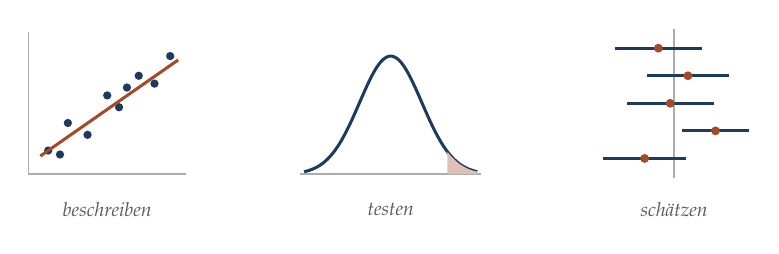
\begin{tikzpicture}[scale=1.0]
% Punktwolke mit Gerade
\begin{scope}[xshift=-3.6cm]
\draw[grau!50, line width=0.6pt] (-1.0,-0.85) -- (-1.0,0.95);
\draw[grau!50, line width=0.6pt] (-1.0,-0.85) -- (1.0,-0.85);
\foreach \x/\y in {-0.75/-0.55, -0.5/-0.2, -0.25/-0.35, 0/0.15, 0.15/0.0, 0.4/0.4, 0.6/0.3, 0.8/0.65, -0.6/-0.6, 0.25/0.25}
  \fill[tief] (\x,\y) circle (1.5pt);
\draw[akzent, line width=1.1pt] (-0.85,-0.62) -- (0.9,0.6);
\node[font=\scriptsize\itshape, color=grau] at (0,-1.3) {beschreiben};
\end{scope}
% Glockenkurve mit Schwanz
\begin{scope}
\draw[grau!50, line width=0.6pt] (-1.15,-0.85) -- (1.15,-0.85);
\draw[tief, line width=1.1pt, smooth, samples=60, domain=-1.1:1.1]
  plot (\x, {-0.85 + 1.5*exp(-3.2*\x*\x)});
\fill[akzent!35] (0.72,-0.85) -- plot[smooth, samples=20, domain=0.72:1.1] (\x, {-0.85+1.5*exp(-3.2*\x*\x)}) -- (1.1,-0.85) -- cycle;
\node[font=\scriptsize\itshape, color=grau] at (0,-1.3) {testen};
\end{scope}
% Konfidenzintervalle
\begin{scope}[xshift=3.6cm]
\draw[grau!50, line width=0.6pt] (0,-0.9) -- (0,1.0);
\foreach \y/\a/\b in {0.75/-0.75/0.35, 0.4/-0.35/0.7, 0.05/-0.6/0.5, -0.3/0.1/0.95, -0.65/-0.9/0.15} {
  \draw[tief, line width=1.0pt] (\a,\y) -- (\b,\y);
  \fill[akzent] ({(\a+\b)/2},\y) circle (1.6pt);
}
\node[font=\scriptsize\itshape, color=grau] at (0,-1.3) {schätzen};
\end{scope}
\end{tikzpicture}

\vspace{1.4cm}
{\large\color{grau} Von der Häufigkeitstabelle bis zur kausalen Inferenz}\\[6pt]
{\color{grau} Jeder Schritt erklärt. Mit vollständig durchgerechneten Übungsaufgaben.}\\[1.9cm]
{\small\color{grau} Stand der Forschung: August 2026}
\end{titlepage}
\thispagestyle{empty}
\vspace*{\fill}
\begin{flushleft}
{\small\color{grau}
\textbf{\color{tief}Mathematik von Grund auf} --- Band 17\\[2pt]
\textit{Was die Zahlen hergeben} $\cdot$ Statistik\\[14pt]

Herausgeber und Urheber: Jürgen Maier\\[2pt]
Entstanden 2026 in Zusammenarbeit mit Claude (Anthropic); Konzeption, Vorgaben, Prüfung und Herausgeberschaft: Jürgen Maier.\\[14pt]

\textbf{Lizenz}\\[2pt]
Dieses Werk ist lizenziert unter einer Creative-Commons-Lizenz \textbf{Namensnennung -- Weitergabe unter gleichen Bedingungen 4.0 International (CC BY-SA 4.0)}. Sie dürfen das Werk vervielfältigen, verbreiten, bearbeiten und auch kommerziell nutzen, sofern Sie den Urheber nennen und Bearbeitungen unter derselben Lizenz weitergeben.\\[2pt]
Lizenztext: \texttt{https://creativecommons.org/licenses/by-sa/4.0/legalcode.de}\\[14pt]

\textbf{Quellen und Fassungen}\\[2pt]
Quelltexte, Simulationen, Fehlermeldungen und aktuelle Fassungen aller Bände:\\
\texttt{https://github.com/juergenmaier2026/mathematik-von-grund-auf}\\[2pt]
Dauerhaft archiviert bei Zenodo: \texttt{https://doi.org/10.5281/zenodo.23698547}\\[14pt]

\textbf{Zitiervorschlag}\\[2pt]
Maier, J. (2026). \textit{Mathematik von Grund auf, Band 17: Was die Zahlen hergeben}. Fassung 1.0.1. \texttt{https://doi.org/10.5281/zenodo.23698547}\\[14pt]

Satz: \LaTeX{} mit Palatino. Fassung 1.0.1, Oktober 2026. 282 Seiten.
}
\end{flushleft}
\vspace*{1.5cm}

\tableofcontents
\mainmatter

\chapter*{Vorwort: Das schwierigste Gebiet}
\addcontentsline{toc}{chapter}{Vorwort}
\markboth{Vorwort}{Vorwort}

Die Statistik ist der einzige Teil der Mathematik, den fast jeder anwendet und fast niemand versteht. Das ist keine Polemik, sondern eine empirisch gut belegte Aussage --- und der Grund, warum dieser Band anders gebaut ist als seine Vorgänger.

\begin{merksatz}
\boxtitel{Zwei Befunde, die am Anfang stehen sollten}
\begin{center}
\begin{minipage}{0.9\textwidth}
\textbf{Erstens.} Befragungen unter Wissenschaftlerinnen und Wissenschaftlern, die regelmäßig Statistik anwenden, zeigen seit Jahrzehnten dasselbe Bild: Ein erheblicher Teil kann den $p$-Wert nicht korrekt definieren. In einer vielzitierten Untersuchung an Medizinerinnen und Medizinern wählte die Mehrheit mindestens eine falsche von sechs vorgelegten Deutungen als richtig.

\textbf{Zweitens.} Dasselbe gilt für das Konfidenzintervall. Die verbreitete Deutung --- \enquote{der wahre Wert liegt mit $95\,\%$ Wahrscheinlichkeit in diesem Intervall} --- ist falsch, und zwar nicht in einem spitzfindigen Sinn.
\end{minipage}
\end{center}

\begin{center}
\begin{minipage}{0.88\textwidth}
\kursiv{Beide Begriffe werden in diesem Band vollständig hergeleitet, und beide bekommen einen eigenen Warnkasten, der die falschen Deutungen einzeln durchgeht. Wenn Sie nach Kapitel~6 und Kapitel~7 sagen können, was ein $p$-Wert und ein Konfidenzintervall \kursiv{nicht} sind, hat der Band seinen Zweck erfüllt.}
\end{minipage}
\end{center}
\end{merksatz}

\section*{Warum das so ist}

Es liegt nicht an mangelnder Sorgfalt. Es liegt daran, dass die Statistik zwei Dinge vermischt, die in der übrigen Mathematik getrennt bleiben.

\begin{merksatz}
\boxtitel{Die zwei Hälften}
\begin{center}
\renewcommand{\arraystretch}{1.55}
\begin{tabular}{@{}P{2.6cm}P{6.0cm}@{}}
\toprule
\textbf{Die Rechnung} & Ist gewöhnliche Mathematik. Sie lässt sich beweisen, und dieser Band beweist sie.\\
\textbf{Das Urteil} & Ob ein Verfahren im vorliegenden Fall \kursiv{anwendbar} ist, folgt aus keiner Rechnung. Es ist eine Entscheidung über die Wirklichkeit.\\
\bottomrule
\end{tabular}
\end{center}

\begin{center}
\begin{minipage}{0.88\textwidth}
\kursiv{In Band 16 konnte man sich auf die Definitionen zurückziehen: Ein Graph \kursiv{ist} ein Paar $(V,E)$, basta. Hier steht vor jeder Rechnung die Frage, ob die Voraussetzungen zutreffen --- und diese Frage beantwortet die Statistik nicht, sondern das Fach, aus dem die Daten kommen.}
\end{minipage}
\end{center}
\end{merksatz}

\begin{warnung}
\boxtitelr{Die Folge: ein Band mit doppelter Buchführung}
Zu jedem Verfahren gehören in diesem Band drei Dinge:

\begin{center}
\renewcommand{\arraystretch}{1.5}
\begin{tabular}{@{}P{2.4cm}P{6.2cm}@{}}
\toprule
\textbf{Die Herleitung} & Woher die Formel kommt, vollständig nachgerechnet.\\
\textbf{Die Voraussetzungen} & Was gelten muss, damit sie gilt --- ausdrücklich aufgezählt.\\
\textbf{Der Bruchfall} & Was geschieht, wenn eine Voraussetzung verletzt ist. Meist ein Rechenbeispiel.\\
\bottomrule
\end{tabular}
\end{center}

\begin{center}
\begin{minipage}{0.88\textwidth}
\kursiv{Der dritte Punkt fehlt in den meisten Lehrbüchern, und er ist der wichtigste. Ein Verfahren, dessen Bruchverhalten man nicht kennt, wendet man blind an.}
\end{minipage}
\end{center}
\end{warnung}

\section*{Was Sie mitbringen müssen}

\begin{merksatz}
\boxtitel{Die Voraussetzungen}
\begin{center}
\renewcommand{\arraystretch}{1.5}
\begin{tabular}{@{}P{3.4cm}P{5.2cm}@{}}
\toprule
\textbf{Schulrechnen} & Bruchrechnung, Wurzeln, Potenzen, Umformen von Gleichungen.\\
\textbf{Summenzeichen} & $\sum$ als Abkürzung für \enquote{addiere alles auf}. Wird in Kapitel~2 noch einmal ausführlich eingeführt.\\
\textbf{Wahrschein\-lichkeit} & Nur die Grundbegriffe, und sie werden in Kapitel~4 wiederholt. Band 4 der Reihe enthält alles ausführlich.\\
\textbf{Integrale} & Erst ab Kapitel~4, und dort nur als Flächenberechnung gedeutet. Wer sie nicht kennt, kommt über die Tabellen durch.\\
\bottomrule
\end{tabular}
\end{center}

\begin{center}
\begin{minipage}{0.88\textwidth}
\kursiv{Dieser Band setzt Band 4 \enquote{Die Vermessung des Zufalls} nicht voraus, verweist aber häufig dorthin. Wer die Wahrscheinlichkeitstheorie dahinter sehen will, findet sie dort; wer nur rechnen will, kommt ohne sie aus.}
\end{minipage}
\end{center}
\end{merksatz}

\section*{Die MOBIL-Studie}

Dieser Band hat eine Besonderheit, die die anderen nicht haben: ein einziges Beispiel, das durch alle fünfzehn Kapitel läuft.

\begin{merksatz}
\boxtitel{Die Studie, die uns begleitet}
\begin{center}
\begin{minipage}{0.9\textwidth}
An einer orthopädischen Klinik wird geprüft, ob ein neues Schmerzschema nach Hüftgelenksersatz die Patientinnen und Patienten schneller wieder auf die Beine bringt als das bisherige.

$120$ Personen werden zufällig auf zwei Gruppen verteilt:
\end{minipage}
\end{center}

\begin{center}
\renewcommand{\arraystretch}{1.5}
\begin{tabular}{@{}P{2.0cm}P{2.0cm}P{4.0cm}@{}}
\toprule
\textbf{Gruppe A} & $60$ Personen & bisheriges Schema\\
\textbf{Gruppe B} & $60$ Personen & neues Schema\\
\bottomrule
\end{tabular}
\end{center}

\schritt{Was erhoben wird}
\begin{center}
{\small
\renewcommand{\arraystretch}{1.45}
\begin{tabular}{@{}P{3.4cm}P{2.4cm}P{2.6cm}@{}}
\toprule
\textbf{Merkmal} & \textbf{Kurzname} & \textbf{Werte}\\
\midrule
Schmerz nach $24$ h & \code{NRS24} & $0$ bis $10$\\
Zeit bis zur Mobilisation & \code{MOB} & Stunden\\
Zusätzliche Schmerzmittel & \code{BEDARF} & ja / nein\\
Zufriedenheit & \code{ZUFR} & $1$ bis $5$\\
Alter & \code{ALTER} & Jahre\\
Geschlecht & \code{GESCHL} & w / m\\
Operationsdauer & \code{OPDAUER} & Minuten\\
\bottomrule
\end{tabular}}
\end{center}

\begin{center}
\begin{minipage}{0.88\textwidth}
\kursiv{Die Studie ist erfunden, die Zahlen sind es auch. Sie sind aber so gewählt, dass sie sich von Hand rechnen lassen und dass die Ergebnisse realistisch ausfallen. Jedes Verfahren dieses Bandes wird an ihr vorgeführt.}
\end{minipage}
\end{center}
\end{merksatz}

\begin{merksatz}
\boxtitel{Warum ein durchgehendes Beispiel}
\begin{center}
\renewcommand{\arraystretch}{1.5}
\begin{tabular}{@{}P{3.0cm}P{5.6cm}@{}}
\toprule
\textbf{Vergleich\-barkeit} & Verschiedene Verfahren auf dieselben Daten angewandt geben verschiedene Antworten. Das sieht man nur, wenn die Daten dieselben bleiben.\\
\textbf{Der ganze Weg} & Von der Häufigkeitstabelle über den Test bis zur Metaanalyse --- an einem einzigen Vorhaben.\\
\textbf{Die Fallen bleiben sichtbar} & Wer in Kapitel~2 den Mittelwert des NRS gebildet hat, erfährt in Kapitel~9, warum das fragwürdig war.\\
\bottomrule
\end{tabular}
\end{center}
\end{merksatz}

\section*{Drei Warnungen}

\begin{warnung}
\boxtitelr{Erstens: Signifikanz ist nicht Bedeutsamkeit}
Das Wort \enquote{signifikant} bedeutet in der Statistik etwas anderes als in der Umgangssprache. Es heißt: \kursiv{Ein Ergebnis dieser Art wäre unter der Nullhypothese selten.} Es heißt nicht: wichtig, groß, klinisch bedeutsam oder gar bewiesen.

Bei genügend großer Stichprobe wird jeder noch so winzige Unterschied signifikant. Kapitel~7 rechnet das vor.
\end{warnung}

\begin{warnung}
\boxtitelr{Zweitens: Kein Test beweist die Nullhypothese}
Ein nicht signifikantes Ergebnis heißt \kursiv{nicht}, dass kein Unterschied besteht. Es heißt nur, dass die Daten nicht ausreichen, um einen nachzuweisen.

\enquote{Wir konnten keinen Unterschied zeigen} und \enquote{Es gibt keinen Unterschied} sind verschiedene Aussagen. Die Verwechslung ist der häufigste Fehler in medizinischen Veröffentlichungen.
\end{warnung}

\begin{warnung}
\boxtitelr{Drittens: Die Rechnung ist der kleinste Teil}
Jedes Verfahren dieses Bandes lässt sich in einer Zeile aufrufen. Die Rechnung dauert Millisekunden.

Die Arbeit steckt vorher --- in der Frage, welches Verfahren passt --- und nachher --- in der Frage, was das Ergebnis bedeutet. Ein Lehrbuch, das nur die Rechnung zeigt, bereitet auf den unwichtigen Teil vor.

\begin{center}
\begin{minipage}{0.88\textwidth}
\kursiv{Aus demselben Grund enthält dieser Band fast keinen Programmcode. Wo er nützlich ist, steht ein kurzer Technikkasten mit zwei bis drei Zeilen R --- zur Kontrolle der Handrechnung, nicht als Ersatz für sie.}
\end{minipage}
\end{center}
\end{warnung}

\section*{Der Aufbau}

\begin{merksatz}
\boxtitel{Sechs Teile, fünfzehn Kapitel}
\begin{center}
{\small
\renewcommand{\arraystretch}{1.45}
\begin{tabular}{@{}P{1.0cm}P{3.2cm}P{4.4cm}@{}}
\toprule
\textbf{Teil} & \textbf{Thema} & \textbf{Die Leitfrage}\\
\midrule
I & Beschreiben (1--3) & Was steht in den Daten?\\
II & Schätzen (4--6) & Was sagen sie über die Grundgesamtheit?\\
III & Testen (7--9) & Wann ist ein Unterschied mehr als Zufall?\\
IV & Modelle (10--11) & Wie hängen mehrere Größen zusammen?\\
V & Medizin (12--14) & Was ist beim Menschen anders?\\
VI & Stand (15) & Was ist heute strittig?\\
\bottomrule
\end{tabular}}
\end{center}
\end{merksatz}

\vspace{10pt}
\begin{flushright}
\itshape\color{grau}
Die Formel ist das Leichte.\\
Die Frage, ob sie hier gilt,\\
ist das Eigentliche.
\end{flushright}

\part{Beschreiben}

\chapter{Daten, Skalen und die erste Falle}

\section{Was ein Datensatz ist}

Beginnen wir beim Gegenstand. Alles Weitere setzt voraus, dass klar ist, worüber gesprochen wird.

\begin{definition}
\boxtitelm{Definition 1.1 --- Merkmal, Ausprägung, Beobachtung}
\begin{itemize}[leftmargin=1.4em, itemsep=4pt]
\item Ein \Begriff{Merkmal} ist eine Eigenschaft, die an jedem Untersuchungsobjekt erhoben wird --- etwa das Alter oder das Geschlecht.
\item Die möglichen Werte eines Merkmals heißen seine \Begriff{Ausprägungen}.
\item Eine \Begriff{Beobachtung} ist ein einzelnes Untersuchungsobjekt zusammen mit allen an ihm erhobenen Werten.
\item Die \Begriff{Stichprobe} ist die Gesamtheit der Beobachtungen; ihr Umfang heißt $n$.
\end{itemize}
\end{definition}

\begin{merksatz}
\boxtitel{Die Datenmatrix}
Man ordnet die Daten in einer Tabelle an: eine Zeile je Beobachtung, eine Spalte je Merkmal.

\begin{center}
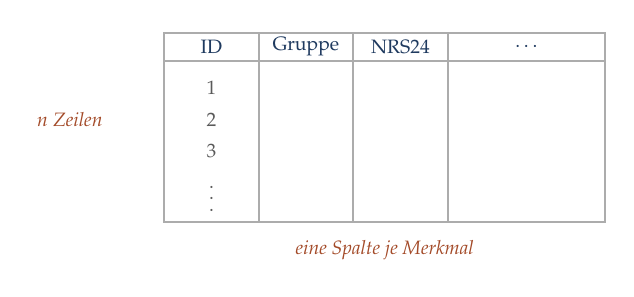
\begin{tikzpicture}[scale=1.0]
\draw[grau!50, line width=0.7pt] (-2.8,-1.3) rectangle (2.8,1.1);
\draw[grau!50, line width=0.7pt] (-2.8,0.75) -- (2.8,0.75);
\foreach \x in {-1.6,-0.4,0.8} \draw[grau!50, line width=0.7pt] (\x,-1.3) -- (\x,1.1);
\node[font=\scriptsize, color=tief] at (-2.2,0.93) {ID};
\node[font=\scriptsize, color=tief] at (-1.0,0.93) {Gruppe};
\node[font=\scriptsize, color=tief] at (0.2,0.93) {NRS24};
\node[font=\scriptsize, color=tief] at (1.8,0.93) {$\ldots$};
\node[font=\scriptsize, color=grau] at (-2.2,0.4) {$1$};
\node[font=\scriptsize, color=grau] at (-2.2,0.0) {$2$};
\node[font=\scriptsize, color=grau] at (-2.2,-0.4) {$3$};
\node[font=\scriptsize, color=grau] at (-2.2,-0.9) {$\vdots$};
\node[font=\scriptsize\itshape, color=akzent] at (-4.0,0.0) {$n$ Zeilen};
\node[font=\scriptsize\itshape, color=akzent] at (0,-1.65) {eine Spalte je Merkmal};
\end{tikzpicture}
\end{center}

\begin{center}
\begin{minipage}{0.88\textwidth}
\kursiv{Diese Anordnung ist keine Formsache. Fast jeder Fehler in der Datenauswertung lässt sich darauf zurückführen, dass Zeilen und Spalten verwechselt werden --- dass etwa über Merkmale gemittelt wird statt über Beobachtungen, oder dass eine Person versehentlich zweimal als Zeile erscheint.}
\end{minipage}
\end{center}
\end{merksatz}

\begin{merksatz}
\boxtitel{Der Auszug aus der MOBIL-Studie}
Für die Handrechnungen dieses Bandes benutzen wir durchgehend denselben Ausschnitt aus zwölf Beobachtungen --- sechs je Gruppe.

\begin{center}
{\small
\renewcommand{\arraystretch}{1.32}
\begin{tabular}{@{}P{0.9cm}P{1.3cm}P{1.2cm}P{1.5cm}P{1.3cm}P{1.5cm}@{}}
\toprule
\textbf{ID} & \textbf{Gruppe} & \textbf{Alter} & \textbf{Geschl.} & \textbf{NRS24} & \textbf{MOB (h)}\\
\midrule
$1$ & A & $68$ & w & $5$ & $26$\\
$2$ & A & $74$ & m & $3$ & $19$\\
$3$ & A & $61$ & w & $6$ & $31$\\
$4$ & A & $79$ & m & $4$ & $24$\\
$5$ & A & $70$ & w & $7$ & $35$\\
$6$ & A & $65$ & m & $5$ & $22$\\
\midrule
$7$ & B & $72$ & w & $3$ & $18$\\
$8$ & B & $66$ & m & $2$ & $15$\\
$9$ & B & $81$ & w & $4$ & $21$\\
$10$ & B & $69$ & m & $3$ & $17$\\
$11$ & B & $75$ & w & $5$ & $23$\\
$12$ & B & $63$ & m & $2$ & $14$\\
\bottomrule
\end{tabular}}
\end{center}

\begin{center}
\begin{minipage}{0.88\textwidth}
\kursiv{Merken Sie sich die Tabelle nicht --- sie wird in jedem Kapitel wieder abgedruckt, wo sie gebraucht wird. Merken Sie sich nur, dass es dieselbe bleibt.}
\end{minipage}
\end{center}
\end{merksatz}

\section{Skalenniveaus}

Nun die zentrale Unterscheidung dieses Kapitels. Sie entscheidet darüber, welche Rechnungen mit einem Merkmal überhaupt sinnvoll sind.

\begin{merksatz}
\boxtitel{Die Grundidee}
Zahlen in einer Datentabelle sind nicht immer Zahlen im Sinne der Arithmetik. Manchmal sind sie bloße \kursiv{Namen}, die man ebenso gut durch Buchstaben ersetzen könnte.

\begin{center}
\renewcommand{\arraystretch}{1.5}
\begin{tabular}{@{}P{3.0cm}P{5.6cm}@{}}
\toprule
Stations\-nummer $3$ & Die $3$ ist ein Name. \enquote{Station $3$ plus Station $5$} ergibt keinen Sinn.\\
Schmerz $3$ auf der NRS & Die $3$ bedeutet \enquote{weniger als $4$}, aber nicht \enquote{halb so viel wie $6$}.\\
Alter $3$ Jahre & Hier ist alles erlaubt: Summen, Verhältnisse, Mittelwerte.\\
\bottomrule
\end{tabular}
\end{center}

\begin{center}
\begin{minipage}{0.88\textwidth}
\kursiv{Die Frage lautet also: Welche Rechenoperationen bewahren die Auskunft, die in der Zahl steckt? Das ist der Kern des Skalenbegriffs, und so wird er im Folgenden auch definiert.}
\end{minipage}
\end{center}
\end{merksatz}

\begin{definition}
\boxtitelm{Definition 1.2 --- die vier Skalenniveaus}
Ein Merkmal heißt

\begin{itemize}[leftmargin=1.4em, itemsep=5pt]
\item \Begriff{nominalskaliert}, wenn seine Ausprägungen nur unterschieden, aber nicht geordnet werden können. Die Auskunft bleibt erhalten unter jeder \kursiv{umkehrbaren Umbenennung}.

\item \Begriff{ordinalskaliert}, wenn die Ausprägungen zusätzlich in eine Rangfolge gebracht werden können, die Abstände aber nicht deutbar sind. Die Auskunft bleibt erhalten unter jeder \kursiv{streng wachsenden} Umformung.

\item \Begriff{intervallskaliert}, wenn zusätzlich die Abstände deutbar sind, der Nullpunkt aber willkürlich ist. Erhalten unter Umformungen $x \mapsto a x + b$ mit $a > 0$.

\item \Begriff{verhältnisskaliert}, wenn zusätzlich ein natürlicher Nullpunkt vorliegt, so dass Verhältnisse deutbar sind. Erhalten nur unter $x \mapsto a x$ mit $a > 0$.
\end{itemize}
\end{definition}

\begin{merksatz}
\boxtitel{Was diese Definition wirklich sagt}
Sie definiert das Skalenniveau nicht über die Zahlen, sondern über die \kursiv{erlaubten Umformungen}. Das ist ungewöhnlich und lohnt eine Erläuterung.

\schritt{Am Beispiel der Temperatur}
Celsius und Fahrenheit hängen zusammen über
\[ F = 1{,}8 \cdot C + 32 . \]
Das ist eine Umformung der Bauart $x \mapsto ax+b$. Beide Skalen enthalten dieselbe Auskunft --- also ist alles, was bei dieser Umformung erhalten bleibt, eine echte Eigenschaft der Temperatur, und alles andere ein Artefakt der Skala.

\schritt{Die Probe}
\begin{center}
\renewcommand{\arraystretch}{1.48}
\begin{tabular}{@{}P{3.0cm}P{2.2cm}P{3.0cm}@{}}
\toprule
\textbf{Aussage} & \textbf{Celsius} & \textbf{Fahrenheit}\\
\midrule
$20^\circ$ wärmer als $10^\circ$ & ja & $68 > 50$: ja \checkmark\\
Abstand $10$--$20$ $=$ Abstand $30$--$40$ & ja & $18 = 18$: ja \checkmark\\
$20^\circ$ ist doppelt so warm wie $10^\circ$ & \enquote{$2\times$} & $68/50 = 1{,}36$: \textcolor{akzent}{\textbf{nein}}\\
\bottomrule
\end{tabular}
\end{center}

Die dritte Zeile zeigt: Das Verhältnis ist \kursiv{keine} Eigenschaft der Temperatur, sondern hängt davon ab, wo man die Null hingelegt hat. Genau deshalb ist Celsius intervall- und nicht verhältnisskaliert.

\begin{center}
\begin{minipage}{0.88\textwidth}
\kursiv{Bei der absoluten Temperatur in Kelvin ist das anders: Dort liegt die Null am physikalisch ausgezeichneten Punkt, und $200$ K sind tatsächlich doppelt so warm wie $100$ K. Kelvin ist verhältnisskaliert, Celsius nicht --- obwohl beides Temperaturen sind.}
\end{minipage}
\end{center}
\end{merksatz}

\begin{merksatz}
\boxtitel{Was auf welcher Skala erlaubt ist}
\begin{center}
{\small
\renewcommand{\arraystretch}{1.42}
\begin{tabular}{@{}P{3.2cm}P{1.2cm}P{1.2cm}P{1.4cm}P{1.4cm}@{}}
\toprule
& \textbf{nom.} & \textbf{ord.} & \textbf{interv.} & \textbf{verh.}\\
\midrule
Gleichheit prüfen & \textcolor{gruen}{ja} & \textcolor{gruen}{ja} & \textcolor{gruen}{ja} & \textcolor{gruen}{ja}\\
Häufigkeiten zählen & \textcolor{gruen}{ja} & \textcolor{gruen}{ja} & \textcolor{gruen}{ja} & \textcolor{gruen}{ja}\\
Modus & \textcolor{gruen}{ja} & \textcolor{gruen}{ja} & \textcolor{gruen}{ja} & \textcolor{gruen}{ja}\\
Ordnen, Rangzahlen & \textcolor{akzent}{nein} & \textcolor{gruen}{ja} & \textcolor{gruen}{ja} & \textcolor{gruen}{ja}\\
Median, Quantile & \textcolor{akzent}{nein} & \textcolor{gruen}{ja} & \textcolor{gruen}{ja} & \textcolor{gruen}{ja}\\
Differenzen bilden & \textcolor{akzent}{nein} & \textcolor{akzent}{nein} & \textcolor{gruen}{ja} & \textcolor{gruen}{ja}\\
\textbf{Mittelwert, Varianz} & \textcolor{akzent}{nein} & \textcolor{akzent}{\textbf{nein}} & \textcolor{gruen}{ja} & \textcolor{gruen}{ja}\\
Verhältnisse bilden & \textcolor{akzent}{nein} & \textcolor{akzent}{nein} & \textcolor{akzent}{\textbf{nein}} & \textcolor{gruen}{ja}\\
Variations\-koeffizient & \textcolor{akzent}{nein} & \textcolor{akzent}{nein} & \textcolor{akzent}{nein} & \textcolor{gruen}{ja}\\
\bottomrule
\end{tabular}}
\end{center}

\begin{center}
\begin{minipage}{0.88\textwidth}
\kursiv{Die fett gesetzte Zeile ist die folgenreichste --- und die am häufigsten missachtete. Der nächste Abschnitt geht ihr nach.}
\end{minipage}
\end{center}
\end{merksatz}

\begin{merksatz}
\boxtitel{Die Merkmale der MOBIL-Studie eingeordnet}
\begin{center}
{\small
\renewcommand{\arraystretch}{1.45}
\begin{tabular}{@{}P{2.2cm}P{2.4cm}P{3.6cm}@{}}
\toprule
\textbf{Merkmal} & \textbf{Skala} & \textbf{Begründung}\\
\midrule
\code{GESCHL} & nominal & keine Ordnung\\
\code{GRUPPE} & nominal & A und B sind Namen\\
\code{NRS24} & \textbf{ordinal} & Rangfolge ja, Abstände nein\\
\code{ZUFR} & ordinal & wie NRS\\
\code{BEDARF} & nominal (binär) & ja / nein\\
\code{ALTER} & verhältnis & natürlicher Nullpunkt\\
\code{MOB} & verhältnis & $0$ Stunden ist echte Null\\
\code{OPDAUER} & verhältnis & \\
\bottomrule
\end{tabular}}
\end{center}

\schritt{Ein Sonderfall: das binäre Merkmal}
\code{BEDARF} ist nominal mit zwei Ausprägungen. Kodiert man \enquote{ja} als $1$ und \enquote{nein} als $0$, so ist der Mittelwert dieser Kodierung gleich dem \kursiv{Anteil} der Ja-Fälle --- eine sinnvolle Größe.

Das ist kein Widerspruch zur Tabelle oben. Bei zwei Ausprägungen fallen Ordinal-, Intervall- und Verhältnisskala zusammen, weil es nur einen Abstand gibt und er keine Vergleichsgröße hat. Binäre Merkmale sind deshalb der einzige Fall, in dem man ein nominales Merkmal mitteln darf.
\end{merksatz}

\section{Die erste Falle: der Mittelwert ordinaler Daten}

\begin{warnung}
\boxtitelr{Was bei der NRS schiefgeht}
Die \Begriff{numerische Rating-Skala} für Schmerz läuft von $0$ (kein Schmerz) bis $10$ (stärkster vorstellbarer Schmerz). Die Zahlen suggerieren gleiche Abstände. Das ist eine Annahme, keine Messung.

\schritt{Die kritische Frage}
Ist der Unterschied zwischen $2$ und $3$ derselbe wie zwischen $7$ und $8$?

Empirische Untersuchungen zur Schmerzmessung legen nahe: nein. Der Schritt im unteren Bereich wird als kleiner erlebt als der im oberen. Die Skala ist also gestaucht und gedehnt --- ordinal, nicht intervallskaliert.
\end{warnung}

\begin{merksatz}
\boxtitel{Ein Rechenbeispiel, das den Schaden zeigt}
Betrachten wir zwei Personen mit den NRS-Werten $2$ und $8$, und zwei andere mit $5$ und $5$.

\schritt{Nach der üblichen Rechnung}
\[ \MW_1 = \frac{2+8}{2} = 5, \qquad \MW_2 = \frac{5+5}{2} = 5 . \]
Die beiden Paare erscheinen gleich.

\schritt{Mit einer anderen, ebenso zulässigen Kodierung}
Die Ordinalskala erlaubt jede streng wachsende Umbenennung. Wir wählen eine, die dem oberen Bereich mehr Gewicht gibt --- was der Schmerzempfindung näherkommt:
\begin{center}
{\small
\renewcommand{\arraystretch}{1.35}
\begin{tabular}{@{}P{1.6cm}P{0.9cm}P{0.9cm}P{0.9cm}P{0.9cm}P{0.9cm}P{0.9cm}@{}}
\toprule
NRS & $0$ & $2$ & $5$ & $8$ & $10$ & \\
neu & $0$ & $3$ & $12$ & $40$ & $60$ & \\
\bottomrule
\end{tabular}}
\end{center}

\schritt{Dieselbe Rechnung}
\[ \MW_1 = \frac{3+40}{2} = 21{,}5, \qquad \MW_2 = \frac{12+12}{2} = 12 . \]

\schritt{Das Ergebnis}
Nun erscheint das erste Paar deutlich schlechter als das zweite --- bei \kursiv{identischen} Daten.

\begin{center}
\begin{minipage}{0.9\textwidth}
\textbf{Der Vergleich zweier Mittelwerte kann sich umkehren, wenn man die Kodierung ändert. Bei ordinalen Daten ist die Kodierung aber willkürlich. Also ist der Vergleich willkürlich.}
\end{minipage}
\end{center}

\schritt{Was der Median macht}
\[ \Med_1 = \frac{2+8}{2} \ \text{ nach Umkodierung } \ \frac{3+40}{2} \ ? \]
Halt --- bei zwei Werten ist auch der Median ein Mittel aus zweien und leidet unter demselben Problem.

Nehmen wir daher drei Werte: $2, 5, 8$ gegen $5,5,5$.
\begin{center}
\renewcommand{\arraystretch}{1.45}
\begin{tabular}{@{}P{2.6cm}P{2.6cm}P{2.4cm}@{}}
\toprule
& \textbf{Original\-kodierung} & \textbf{neue Kodierung}\\
\midrule
Median $\{2,5,8\}$ & $5$ & $12$\\
Median $\{5,5,5\}$ & $5$ & $12$\\
\midrule
\textbf{Vergleich} & gleich & \textcolor{gruen}{\textbf{gleich}}\\
\bottomrule
\end{tabular}
\end{center}

Der Median ist die \kursiv{mittlere Ausprägung}, und welche das ist, hängt nur von der Rangfolge ab --- nicht von den zugewiesenen Zahlen. Er bleibt unter jeder streng wachsenden Umkodierung derselbe Datenpunkt.
\end{merksatz}

\begin{warnung}
\boxtitelr{Und trotzdem wird gemittelt --- auch in diesem Band}
Die Wirklichkeit der medizinischen Forschung sieht anders aus. NRS-Werte, Likert-Skalen und Scores werden gemittelt, in $t$-Tests gesteckt und in Regressionen verwendet. Auch dieser Band wird es in Kapitel~2 tun.

Das hat Gründe, die man kennen sollte:

\begin{center}
\renewcommand{\arraystretch}{1.5}
\begin{tabular}{@{}P{3.0cm}P{5.6cm}@{}}
\toprule
\textbf{Robustheit} & Simulationsstudien zeigen, dass $t$-Tests auf Likert-Daten meist brauchbare Fehlerraten liefern, solange die Verteilungen ähnlich geformt sind.\\
\textbf{Vergleich\-barkeit} & Die gesamte Literatur rechnet so. Wer es anders macht, ist nicht vergleichbar.\\
\textbf{Es gibt Alternativen} & Verteilungsfreie Verfahren (Kapitel~9) und ordinale Regression (Kapitel~11) kommen ohne die Annahme aus.\\
\bottomrule
\end{tabular}
\end{center}

\begin{center}
\begin{minipage}{0.88\textwidth}
\kursiv{Die ehrliche Haltung ist nicht das Verbot, sondern das Bewusstsein: Wer ordinale Daten mittelt, trifft eine Zusatzannahme über gleiche Abstände. Diese Annahme ist meist unausgesprochen und selten geprüft. Sie \kursiv{kann} vertretbar sein --- aber sie gehört in den Methodenteil, nicht ins Schweigen.}
\end{minipage}
\end{center}
\end{warnung}

\section{Diskret und stetig}

\begin{definition}
\boxtitelm{Definition 1.3}
Ein Merkmal heißt \Begriff{diskret}, wenn seine Ausprägungen abzählbar sind --- etwa ganze Zahlen oder Kategorien. Es heißt \Begriff{stetig}, wenn es grundsätzlich jeden Wert in einem Bereich annehmen kann.
\end{definition}

\begin{warnung}
\boxtitelr{Jede Messung ist in Wahrheit diskret}
Die Mobilisationszeit ist ein stetiges Merkmal: Zwischen $18$ und $19$ Stunden liegen unendlich viele mögliche Werte.

Erhoben wird sie aber in vollen Stunden. Die Daten sind also diskret, obwohl das Merkmal stetig ist.

\begin{center}
\renewcommand{\arraystretch}{1.5}
\begin{tabular}{@{}P{2.6cm}P{6.0cm}@{}}
\toprule
\textbf{Das Merkmal} & stetig --- eine Eigenschaft der Wirklichkeit\\
\textbf{Die Messung} & diskret --- eine Eigenschaft des Messvorgangs\\
\bottomrule
\end{tabular}
\end{center}

Diese Unterscheidung wird in Kapitel~9 wichtig: Verfahren, die auf Rangzahlen beruhen, verlangen, dass keine Bindungen auftreten --- also keine zwei gleichen Werte. Bei grober Rundung treten sie aber ständig auf, und man braucht eine Korrektur.
\end{warnung}

\section{Häufigkeiten}

\begin{definition}
\boxtitelm{Definition 1.4 --- die drei Häufigkeitsbegriffe}
Sei $a$ eine Ausprägung eines Merkmals in einer Stichprobe vom Umfang $n$.
\begin{itemize}[leftmargin=1.4em, itemsep=4pt]
\item Die \Begriff{absolute Häufigkeit} $H(a)$ ist die Anzahl der Beobachtungen mit dieser Ausprägung.
\item Die \Begriff{relative Häufigkeit} ist $h(a) = H(a)/n$.
\item Die \Begriff{kumulierte Häufigkeit} ist die Summe der relativen Häufigkeiten aller Ausprägungen bis einschließlich $a$ --- sinnvoll nur ab Ordinalskala.
\end{itemize}
\end{definition}

\begin{merksatz}
\boxtitel{Die Häufigkeitstabelle für \code{NRS24}}
Wir nehmen alle zwölf Beobachtungen des Auszugs: $5,3,6,4,7,5,3,2,4,3,5,2$.

\schritt{Schritt 1 --- Sortieren}
\[ 2,\ 2,\ 3,\ 3,\ 3,\ 4,\ 4,\ 5,\ 5,\ 5,\ 6,\ 7 \]

\schritt{Schritt 2 --- Auszählen}
\begin{center}
{\small
\renewcommand{\arraystretch}{1.38}
\begin{tabular}{@{}P{1.3cm}P{1.5cm}P{1.9cm}P{2.4cm}@{}}
\toprule
\textbf{NRS} & $H$ & $h$ & \textbf{kumuliert}\\
\midrule
$2$ & $2$ & $2/12 = 0{,}167$ & $0{,}167$\\
$3$ & $3$ & $3/12 = 0{,}250$ & $0{,}417$\\
$4$ & $2$ & $2/12 = 0{,}167$ & $0{,}583$\\
$5$ & $3$ & $3/12 = 0{,}250$ & $0{,}833$\\
$6$ & $1$ & $1/12 = 0{,}083$ & $0{,}917$\\
$7$ & $1$ & $1/12 = 0{,}083$ & $1{,}000$\\
\midrule
\textbf{Summe} & $\mathbf{12}$ & $\mathbf{1{,}000}$ & \\
\bottomrule
\end{tabular}}
\end{center}

\schritt{Die beiden Proben}
Die absoluten Häufigkeiten müssen sich zu $n$ summieren: $2+3+2+3+1+1 = 12$. \checkmark\\
Die relativen zu $1$, und die letzte kumulierte muss $1$ sein. \checkmark

\schritt{Was man daraus abliest}
Die kumulierte Spalte beantwortet Fragen der Art \enquote{Wie viele hatten höchstens $4$?} --- nämlich $58{,}3\,\%$. Solche Fragen sind bei ordinalen Merkmalen zulässig, weil sie nur die Rangfolge benutzen.
\end{merksatz}

\begin{merksatz}
\boxtitel{Getrennt nach Gruppen --- die eigentlich interessante Tabelle}
\begin{center}
{\small
\renewcommand{\arraystretch}{1.38}
\begin{tabular}{@{}P{1.3cm}P{1.4cm}P{1.4cm}P{2.0cm}P{2.0cm}@{}}
\toprule
\textbf{NRS} & $H_A$ & $H_B$ & $h_A$ & $h_B$\\
\midrule
$2$ & $0$ & $2$ & $0{,}00$ & $0{,}33$\\
$3$ & $1$ & $2$ & $0{,}17$ & $0{,}33$\\
$4$ & $1$ & $1$ & $0{,}17$ & $0{,}17$\\
$5$ & $2$ & $1$ & $0{,}33$ & $0{,}17$\\
$6$ & $1$ & $0$ & $0{,}17$ & $0{,}00$\\
$7$ & $1$ & $0$ & $0{,}17$ & $0{,}00$\\
\midrule
\textbf{Summe} & $\mathbf{6}$ & $\mathbf{6}$ & $\mathbf{1{,}00}$ & $\mathbf{1{,}00}$\\
\bottomrule
\end{tabular}}
\end{center}

\begin{center}
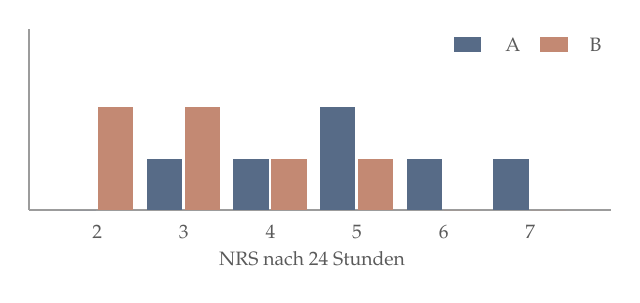
\begin{tikzpicture}[scale=1.0]
\draw[grau!60, line width=0.7pt] (-0.4,0) -- (7.0,0);
\draw[grau!60, line width=0.7pt] (-0.4,0) -- (-0.4,2.3);
\foreach \i/\ha/\hb in {0/0/2, 1/1/2, 2/1/1, 3/2/1, 4/1/0, 5/1/0} {
  \fill[tief!75] (\i*1.1+0.0,0) rectangle (\i*1.1+0.45,\ha*0.65);
  \fill[akzent!65] (\i*1.1+0.48,0) rectangle (\i*1.1+0.93,\hb*0.65);
}
\foreach \i/\lab in {0/2, 1/3, 2/4, 3/5, 4/6, 5/7}
  \node[font=\scriptsize, color=grau] at (\i*1.1+0.47,-0.28) {\lab};
\node[font=\scriptsize, color=grau] at (3.2,-0.62) {NRS nach 24 Stunden};
\fill[tief!75] (5.0,2.0) rectangle (5.35,2.2);
\node[font=\scriptsize, color=grau] at (5.75,2.1) {A};
\fill[akzent!65] (6.1,2.0) rectangle (6.45,2.2);
\node[font=\scriptsize, color=grau] at (6.8,2.1) {B};
\end{tikzpicture}
\end{center}

\begin{center}
\begin{minipage}{0.88\textwidth}
\kursiv{Man sieht mit bloßem Auge, dass die Gruppe B nach links verschoben liegt. Ob dieser Eindruck mehr ist als Zufall bei zwölf Beobachtungen, ist die Frage von Teil~III. Die Beschreibung liefert die Vermutung, nicht den Beleg.}
\end{minipage}
\end{center}
\end{merksatz}

\section{Darstellungen und ihre Fallen}

\begin{warnung}
\boxtitelr{Die abgeschnittene Achse}
\begin{center}
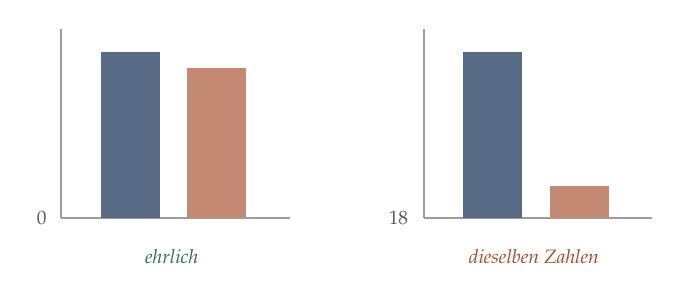
\begin{tikzpicture}[scale=1.0]
\begin{scope}
\draw[grau!60, line width=0.7pt] (-0.3,0) -- (2.6,0);
\draw[grau!60, line width=0.7pt] (-0.3,0) -- (-0.3,2.4);
\fill[tief!75] (0.2,0) rectangle (0.95,2.1);
\fill[akzent!65] (1.3,0) rectangle (2.05,1.9);
\node[font=\scriptsize, color=grau] at (-0.55,0) {$0$};
\node[font=\scriptsize\itshape, color=gruen] at (1.1,-0.5) {ehrlich};
\end{scope}
\begin{scope}[xshift=4.6cm]
\draw[grau!60, line width=0.7pt] (-0.3,0) -- (2.6,0);
\draw[grau!60, line width=0.7pt] (-0.3,0) -- (-0.3,2.4);
\fill[tief!75] (0.2,0) rectangle (0.95,2.1);
\fill[akzent!65] (1.3,0) rectangle (2.05,0.4);
\node[font=\scriptsize, color=grau] at (-0.62,0) {$18$};
\node[font=\scriptsize\itshape, color=akzent] at (1.1,-0.5) {dieselben Zahlen};
\end{scope}
\end{tikzpicture}
\end{center}

Beide Bilder zeigen die Werte $26{,}2$ und $18{,}0$ --- die mittleren Mobilisationszeiten der beiden Gruppen. Rechts beginnt die Achse bei $18$ statt bei $0$, und der Unterschied erscheint als Faktor fünf statt als Faktor $1{,}5$.

\begin{center}
\begin{minipage}{0.88\textwidth}
\kursiv{Die Regel lautet: Bei Balkendiagrammen beginnt die Achse bei null, weil die \kursiv{Balkenlänge} die Größe darstellt. Bei Liniendiagrammen darf man ausschneiden, weil dort die \kursiv{Neigung} die Aussage trägt --- muss es aber kenntlich machen.}
\end{minipage}
\end{center}
\end{warnung}

\begin{warnung}
\boxtitelr{Das Kreisdiagramm}
Kreisdiagramme sind fast immer die schlechtere Wahl. Der Grund ist wahrnehmungspsychologisch: Menschen vergleichen Längen erheblich genauer als Winkel oder Flächen.

\begin{center}
\renewcommand{\arraystretch}{1.5}
\begin{tabular}{@{}P{2.8cm}P{5.8cm}@{}}
\toprule
\textbf{Vertretbar} & Zwei bis drei Kategorien, grobe Anteile, kein Vergleich zwischen Kreisen.\\
\textbf{Ungeeignet} & Mehr als vier Kategorien; Vergleich zweier Kreise; ähnlich große Anteile.\\
\textbf{Unzulässig} & Dreidimensionale Kreise mit Perspektive --- die vorderen Segmente erscheinen systematisch größer.\\
\bottomrule
\end{tabular}
\end{center}

\begin{center}
\begin{minipage}{0.88\textwidth}
\kursiv{Ein gestapelter Balken leistet dasselbe wie ein Kreisdiagramm und lässt sich zwischen Gruppen vergleichen. Es gibt fast keine Lage, in der das Kreisdiagramm die bessere Wahl ist --- und es ist trotzdem die häufigste.}
\end{minipage}
\end{center}
\end{warnung}

\section{Übungsaufgaben}

\begin{aufgabe}
\boxtitel{Aufgabe 1.1 --- Skalenniveaus bestimmen}
Ordnen Sie den folgenden Merkmalen ein Skalenniveau zu und begründen Sie jeweils über die erlaubten Umformungen.

\begin{center}
{\small
\renewcommand{\arraystretch}{1.35}
\begin{tabular}{@{}P{4.0cm}P{4.4cm}@{}}
\toprule
(a) Blutgruppe & (d) ASA-Klassifikation I--IV\\
(b) Körpergröße in cm & (e) Kalenderjahr\\
(c) Postleitzahl & (f) Temperatur in Kelvin\\
\bottomrule
\end{tabular}}
\end{center}

\loesung
\schritt{(a) Blutgruppe --- nominal}
Die Ausprägungen A, B, AB, 0 lassen sich unterscheiden, aber nicht sinnvoll ordnen. Jede umkehrbare Umbenennung --- etwa A$\to$3, B$\to$1 --- bewahrt die gesamte Auskunft. Also nominal.

\schritt{(b) Körpergröße --- verhältnisskaliert}
Null Zentimeter bedeutet \enquote{keine Ausdehnung} und ist nicht willkürlich gewählt. Der Wechsel zu Zoll ist die Umformung $x \mapsto x/2{,}54$ --- von der Bauart $x \mapsto ax$ ohne additiven Teil. Die Aussage \enquote{doppelt so groß} bleibt erhalten. Also verhältnisskaliert.

\schritt{(c) Postleitzahl --- nominal}
Obwohl es Zahlen sind und obwohl sie sogar geografisch geordnet erscheinen: Der Abstand zwischen $10115$ und $10117$ ist keine Größe, und Mittelwerte sind sinnlos. Die Zahl ist ein Name. Also nominal.

\begin{center}
\begin{minipage}{0.86\textwidth}
\kursiv{Dies ist der wichtigste Fall der Aufgabe. Dass ein Merkmal als Zahl vorliegt, sagt über sein Skalenniveau nichts.}
\end{minipage}
\end{center}

\schritt{(d) ASA-Klassifikation --- ordinal}
Die Klassen I bis IV beschreiben zunehmenden Schweregrad --- also geordnet. Ob der Abstand I$\to$II derselbe ist wie III$\to$IV, ist nicht definiert und wäre auch nicht messbar. Jede streng wachsende Umbenennung, etwa $1,2,3,4 \mapsto 1,5,9,40$, bewahrt die Auskunft. Also ordinal.

\schritt{(e) Kalenderjahr --- intervallskaliert}
Abstände sind deutbar: Zwischen 1980 und 2000 liegen ebenso viele Jahre wie zwischen 2000 und 2020.

Der Nullpunkt ist aber gesetzt, nicht gefunden. Das Verhältnis \enquote{2000 ist doppelt so viel wie 1000} ist ohne Bedeutung, und in einer anderen Zeitrechnung fiele es anders aus. Der Wechsel von christlicher zu islamischer Zeitrechnung ist eine Umformung $x \mapsto ax+b$. Also intervallskaliert.

\schritt{(f) Temperatur in Kelvin --- verhältnisskaliert}
Der absolute Nullpunkt ist physikalisch ausgezeichnet. $200$ K haben tatsächlich die doppelte mittlere Teilchenenergie von $100$ K. Also verhältnisskaliert --- im Unterschied zu Celsius.

\schritt{Zusammenfassung}
\begin{center}
\renewcommand{\arraystretch}{1.42}
\begin{tabular}{@{}P{1.0cm}P{2.6cm}P{1.0cm}P{2.6cm}@{}}
\toprule
(a) & nominal & (d) & ordinal\\
(b) & verhältnis & (e) & intervall\\
(c) & nominal & (f) & verhältnis\\
\bottomrule
\end{tabular}
\end{center}
\end{aufgabe}

\begin{aufgabe}
\boxtitel{Aufgabe 1.2 --- Eine Häufigkeitstabelle aufstellen}
Stellen Sie für das Merkmal \code{MOB} des Auszugs eine Häufigkeitstabelle mit Klassenbildung auf. Wählen Sie die Klassen selbst und begründen Sie die Wahl.

\loesung
\schritt{Schritt 1 --- Die Daten}
\[ 26,\ 19,\ 31,\ 24,\ 35,\ 22,\ 18,\ 15,\ 21,\ 17,\ 23,\ 14 \]
Sortiert:
\[ 14,\ 15,\ 17,\ 18,\ 19,\ 21,\ 22,\ 23,\ 24,\ 26,\ 31,\ 35 \]

\schritt{Schritt 2 --- Spannweite und Klassenzahl}
Kleinster Wert $14$, größter $35$, Spannweite $35 - 14 = 21$.

Für die Klassenzahl gibt es Faustregeln. Die bekannteste, die \Begriff{Sturges-Regel}, empfiehlt
\[ k \approx 1 + \log_2 n = 1 + \log_2 12 \approx 1 + 3{,}58 = 4{,}58 , \]
also vier oder fünf Klassen.

Eine zweite Faustregel lautet $k \approx \sqrt{n} = \sqrt{12} \approx 3{,}5$.

Wir wählen $k = 5$ und die Klassenbreite $5$, beginnend bei $12{,}5$ --- so fällt kein Beobachtungswert auf eine Klassengrenze.

\schritt{Schritt 3 --- Die Tabelle}
\begin{center}
{\small
\renewcommand{\arraystretch}{1.38}
\begin{tabular}{@{}P{2.4cm}P{1.2cm}P{1.6cm}P{2.2cm}@{}}
\toprule
\textbf{Klasse} & $H$ & $h$ & \textbf{kumuliert}\\
\midrule
$12{,}5$ bis $17{,}5$ & $3$ & $0{,}250$ & $0{,}250$\\
$17{,}5$ bis $22{,}5$ & $4$ & $0{,}333$ & $0{,}583$\\
$22{,}5$ bis $27{,}5$ & $3$ & $0{,}250$ & $0{,}833$\\
$27{,}5$ bis $32{,}5$ & $1$ & $0{,}083$ & $0{,}917$\\
$32{,}5$ bis $37{,}5$ & $1$ & $0{,}083$ & $1{,}000$\\
\midrule
\textbf{Summe} & $\mathbf{12}$ & $\mathbf{1{,}000}$ & \\
\bottomrule
\end{tabular}}
\end{center}

\schritt{Kontrolle der Zuordnung}
Klasse 1: $14, 15, 17$ --- drei. \checkmark\\
Klasse 2: $18, 19, 21, 22$ --- vier. \checkmark\\
Klasse 3: $23, 24, 26$ --- drei. \checkmark\\
Klasse 4: $31$ --- eine. \checkmark\\
Klasse 5: $35$ --- eine. \checkmark\\
Summe $3+4+3+1+1 = 12$. \checkmark

\schritt{Schritt 4 --- Was die Tabelle zeigt und was sie verdeckt}
Die Verteilung ist \kursiv{rechtsschief}: Die Masse liegt links, einzelne große Werte ziehen nach rechts. Das ist bei Zeitdauern der Regelfall --- nach unten begrenzt die Null, nach oben nichts.

Verdeckt wird die Gruppenzugehörigkeit. Alle vier Werte über $22{,}5$ stammen aus Gruppe A. Eine Tabelle über beide Gruppen zusammen verwischt genau den Unterschied, um den es in der Studie geht.

\begin{center}
\begin{minipage}{0.86\textwidth}
\kursiv{Das ist die wichtigere Lehre dieser Aufgabe: Eine Zusammenfassung ist immer auch ein Weglassen. Die Frage ist nie, ob man Auskunft verliert, sondern welche man verlieren darf.}
\end{minipage}
\end{center}
\end{aufgabe}

\begin{aufgabe}
\boxtitel{Aufgabe 1.3 --- Wann kippt der Vergleich?}
In der Warnung oben kehrte sich ein Mittelwertvergleich durch Umkodierung um. Konstruieren Sie ein eigenes Beispiel: zwei Gruppen zu je drei NRS-Werten, bei denen Gruppe A unter der Standardkodierung besser abschneidet und unter einer zulässigen Umkodierung schlechter.

\loesung
\schritt{Schritt 1 --- Überlegen, was nötig ist}
Damit sich ein Mittelwertvergleich umkehren lässt, müssen die Gruppen sich in der \kursiv{Streuung} unterscheiden: Eine Gruppe braucht extreme Werte, die andere mittlere. Sind beide Gruppen gleich gestreut, wirkt jede Umkodierung auf beide ähnlich.

\schritt{Schritt 2 --- Ein Ansatz}
\[ A: \ 1,\ 5,\ 9 \qquad B: \ 4,\ 5,\ 6 \]

Standardkodierung:
\[ \MW_A = \frac{1+5+9}{3} = 5, \qquad \MW_B = \frac{4+5+6}{3} = 5 . \]
Gleichstand --- das genügt noch nicht. Wir verschieben $A$ leicht nach unten:
\[ A: \ 1,\ 4,\ 9 \quad\Rightarrow\quad \MW_A = \frac{14}{3} = 4{,}67 \;<\; 5 = \MW_B . \]
Also ist $A$ unter der Standardkodierung besser (niedriger Schmerz ist besser).

\schritt{Schritt 3 --- Eine zulässige Umkodierung wählen}
Wir brauchen eine streng wachsende Abbildung, die hohe Werte stark spreizt. Nehmen wir $f(x) = x^2$:
\begin{center}
{\small
\renewcommand{\arraystretch}{1.35}
\begin{tabular}{@{}P{1.2cm}P{0.8cm}P{0.8cm}P{0.8cm}P{0.8cm}P{0.8cm}P{0.8cm}@{}}
\toprule
NRS & $1$ & $4$ & $5$ & $6$ & $9$ & \\
$f$ & $1$ & $16$ & $25$ & $36$ & $81$ & \\
\bottomrule
\end{tabular}}
\end{center}
$f$ ist auf $\{0,\ldots,10\}$ streng wachsend, also eine zulässige Umbenennung einer Ordinalskala.

\schritt{Schritt 4 --- Neu rechnen}
\[ \MW_A^{f} = \frac{1 + 16 + 81}{3} = \frac{98}{3} = 32{,}67 \]
\[ \MW_B^{f} = \frac{16 + 25 + 36}{3} = \frac{77}{3} = 25{,}67 \]

\schritt{Schritt 5 --- Das Ergebnis}
\begin{center}
\renewcommand{\arraystretch}{1.48}
\begin{tabular}{@{}P{2.6cm}P{2.0cm}P{2.0cm}P{1.6cm}@{}}
\toprule
& $\MW_A$ & $\MW_B$ & \textbf{besser}\\
\midrule
Standard & $4{,}67$ & $5{,}00$ & \textbf{A}\\
Quadriert & $32{,}67$ & $25{,}67$ & \textcolor{akzent}{\textbf{B}}\\
\bottomrule
\end{tabular}
\end{center}

Der Vergleich hat sich umgekehrt. \checkmark

\schritt{Schritt 6 --- Die Probe mit dem Median}
\[ \Med_A = 4, \qquad \Med_B = 5 . \]
Nach Umkodierung:
\[ \Med_A^f = 16, \qquad \Med_B^f = 25 . \]
In beiden Fällen ist $A$ besser --- der Median ist stabil, weil er nur die Rangposition benutzt und die Umkodierung die Rangfolge nicht ändert.

\schritt{Nachbemerkung}
Beachten Sie, was das Beispiel braucht: Gruppe A ist stark gestreut ($1$ bis $9$), Gruppe B eng ($4$ bis $6$). In der MOBIL-Studie sind die Streuungen ähnlich --- dort ist das Problem daher weniger scharf. Genau deshalb funktioniert das Mitteln von Likert-Daten in der Praxis oft. Es funktioniert nicht, weil die Annahme richtig wäre, sondern weil die Verletzung meist klein ist.
\end{aufgabe}

\begin{geschichte}
\boxtitelg{Stevens, ein Psychologe und ein Streit, der nie endete}
Die vier Skalenniveaus stammen von \Person{Stanley Smith Stevens}, einem Harvard-Psychologen, der sie 1946 in einem dreiseitigen Aufsatz in \kursiv{Science} vorstellte.

Stevens hatte einen konkreten Anlass. Eine britische Kommission hatte 1940 nach siebenjähriger Beratung erklärt, psychologische Größen seien grundsätzlich nicht messbar, weil sich keine Additivität nachweisen lasse. Stevens antwortete mit einer Umdeutung des Messbegriffs: Messen sei die Zuordnung von Zahlen nach einer Regel --- und je nach Regel bekomme man eben verschiedene Skalentypen, von denen nur die oberen die volle Arithmetik erlaubten.

\begin{center}
\begin{minipage}{0.9\textwidth}
\kursiv{Der Aufsatz ist einer der meistzitierten der Wissenschaftsgeschichte und zugleich einer der umstrittensten. Statistiker wie \Person{John Tukey} und \Person{Paul Velleman} haben eingewandt, das Schema sei zu starr: Es entscheide über die Zulässigkeit eines Verfahrens, ohne die Fragestellung zu kennen. Ihr Argument lautet, ein Verfahren sei zulässig, wenn es zu einer sinnvollen Antwort führe --- und das hänge nicht nur an der Skala.}
\end{minipage}
\end{center}

Der Streit ist bis heute nicht entschieden. Dieser Band folgt Stevens als \kursiv{Orientierung} und Velleman als \kursiv{Korrektiv}: Das Schema sagt, wo man hinsehen muss --- nicht, was man tun darf.
\end{geschichte}

\begin{forschung}
\boxtitelp{Wie mit Likert-Daten heute umgegangen wird}
Die Frage, ob man ordinale Bewertungsskalen mitteln darf, ist Gegenstand einer umfangreichen Simulationsliteratur.

\begin{center}
{\small
\renewcommand{\arraystretch}{1.45}
\begin{tabular}{@{}P{2.8cm}P{5.4cm}@{}}
\toprule
\textbf{Befund} & Der $t$-Test hält bei Likert-Daten sein Niveau meist gut ein, solange die Gruppen ähnlich schiefe Verteilungen haben.\\
\textbf{Die Ausnahme} & Bei gegenläufiger Schiefe oder starken Deckeneffekten kann die Fehlerrate deutlich abweichen.\\
\textbf{Der Trend} & Ordinale Regressionsmodelle --- kumulative Logit-Modelle --- setzen sich langsam durch; sie kommen ohne die Abstandsannahme aus.\\
\bottomrule
\end{tabular}}
\end{center}

\begin{center}
\begin{minipage}{0.88\textwidth}
\kursiv{Ein \Begriff{Deckeneffekt} liegt vor, wenn viele Werte am oberen Rand der Skala liegen. Bei postoperativen Schmerzscores tritt regelmäßig das Gegenteil auf --- ein Bodeneffekt bei null ---, sobald die Analgesie gut wirkt. Dann sind die Verteilungen stark schief, und die Warnung aus der zweiten Zeile greift. Kapitel~9 behandelt, was man stattdessen tut.}
\end{minipage}
\end{center}
\end{forschung}

\begin{merksatz}
\boxtitel{Was Sie jetzt können}
\begin{center}
\renewcommand{\arraystretch}{1.5}
\begin{tabular}{@{}P{3.0cm}P{5.6cm}@{}}
\toprule
\textbf{Definition 1.1} & Merkmal, Ausprägung, Beobachtung, Datenmatrix\\
\textbf{Definition 1.2} & Die vier Skalenniveaus --- über erlaubte Umformungen\\
\textbf{Die Tabelle} & Welche Kennzahl auf welcher Skala zulässig ist\\
\textbf{Die erste Falle} & Mittelwerte ordinaler Daten sind kodierungsabhängig\\
\textbf{Definition 1.4} & Absolute, relative und kumulierte Häufigkeit\\
\textbf{Zwei Darstellungsfallen} & Abgeschnittene Achse, Kreisdiagramm\\
\bottomrule
\end{tabular}
\end{center}

\begin{center}
\begin{minipage}{0.88\textwidth}
\kursiv{Im nächsten Kapitel fassen wir eine Häufigkeitsverteilung in wenigen Zahlen zusammen --- und sehen an einem berühmten Beispiel, wie viel dabei verlorengehen kann.}
\end{minipage}
\end{center}
\end{merksatz}

\chapter{Lage und Streuung}

\section{Das Summenzeichen}

Bevor wir rechnen, ein Werkzeug. Es sieht harmloser aus, als es ist --- die meisten Formeln dieses Bandes lassen sich ohne es nicht schreiben.

\begin{definition}
\boxtitelm{Definition 2.1 --- Summenzeichen}
Für Zahlen $x_1, x_2, \ldots, x_n$ schreibt man
\[ \sum_{i=1}^{n} x_i \;=\; x_1 + x_2 + \cdots + x_n . \]
Der Buchstabe $i$ heißt \Begriff{Laufindex}, die $1$ unten die \Begriff{untere Grenze}, das $n$ oben die \Begriff{obere Grenze}.
\end{definition}

\begin{merksatz}
\boxtitel{Wie man es liest}
\begin{center}
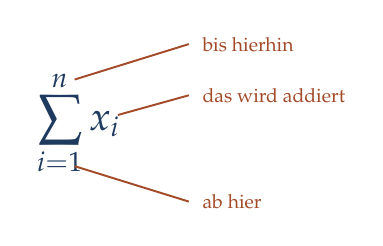
\begin{tikzpicture}[scale=1.0]
\node[font=\Large, color=tief] at (0,0) {$\displaystyle\sum_{i=1}^{n} x_i$};
\draw[akzent, line width=0.7pt] (-0.05,0.55) -- (1.4,1.0);
\node[font=\scriptsize, color=akzent, anchor=west] at (1.45,1.0) {bis hierhin};
\draw[akzent, line width=0.7pt] (-0.05,-0.55) -- (1.4,-1.0);
\node[font=\scriptsize, color=akzent, anchor=west] at (1.45,-1.0) {ab hier};
\draw[akzent, line width=0.7pt] (0.5,0.1) -- (1.4,0.35);
\node[font=\scriptsize, color=akzent, anchor=west] at (1.45,0.35) {das wird addiert};
\end{tikzpicture}
\end{center}

\schritt{An einem Beispiel}
Für die Mobilisationszeiten der Gruppe A --- $x_1 = 26$, $x_2 = 19$, $x_3 = 31$, $x_4 = 24$, $x_5 = 35$, $x_6 = 22$ --- ist
\[ \sum_{i=1}^{6} x_i = 26+19+31+24+35+22 = 157 . \]
\end{merksatz}

\begin{merksatz}
\boxtitel{Drei Regeln, die ständig gebraucht werden}
\begin{center}
\renewcommand{\arraystretch}{1.6}
\begin{tabular}{@{}P{4.4cm}P{4.0cm}@{}}
\toprule
$\displaystyle\sum_{i=1}^n (x_i + y_i) = \sum_{i=1}^n x_i + \sum_{i=1}^n y_i$ & Summen trennen\\
$\displaystyle\sum_{i=1}^n c\,x_i = c \sum_{i=1}^n x_i$ & Faktor herausziehen\\
$\displaystyle\sum_{i=1}^n c = n\,c$ & Konstante $n$-mal addiert\\
\bottomrule
\end{tabular}
\end{center}

\schritt{Warum die dritte Regel stimmt}
Der Ausdruck $\sum_{i=1}^n c$ bedeutet: Addiere den Wert $c$, und zwar für $i=1$, für $i=2$, und so fort bis $i=n$. Das sind $n$ Summanden, jeder gleich $c$.

\begin{center}
\begin{minipage}{0.88\textwidth}
\kursiv{Die dritte Regel ist die, die beim Nachrechnen am häufigsten übersehen wird --- weil im Summanden kein $i$ vorkommt und man versucht ist, die Summe ganz zu ignorieren.}
\end{minipage}
\end{center}
\end{merksatz}

\section{Der Mittelwert}

\begin{definition}
\boxtitelm{Definition 2.2 --- arithmetisches Mittel}
\[ \MW \;=\; \frac{1}{n}\sum_{i=1}^{n} x_i . \]
\end{definition}

\begin{merksatz}
\boxtitel{Satz 2.3 --- Die Abweichungen summieren sich zu null}
\[ \sum_{i=1}^n (x_i - \MW) = 0 . \]

\schritt{Beweis}
Wir wenden die Regeln aus Abschnitt 2.1 an:
\begin{align*}
\sum_{i=1}^n (x_i - \MW) &= \sum_{i=1}^n x_i \;-\; \sum_{i=1}^n \MW && \text{(erste Regel)}\\
&= \sum_{i=1}^n x_i \;-\; n\,\MW && \text{(dritte Regel; } \MW \text{ hängt nicht von } i \text{ ab)}\\
&= \sum_{i=1}^n x_i \;-\; n \cdot \frac{1}{n}\sum_{i=1}^n x_i && \text{(Definition)}\\
&= \sum_{i=1}^n x_i - \sum_{i=1}^n x_i \;=\; 0 . \qquad \blacksquare
\end{align*}

\schritt{Die Deutung}
Der Mittelwert ist der \kursiv{Schwerpunkt} der Daten: Legt man an jeden Datenpunkt ein gleiches Gewicht auf einen Balken, so balanciert er genau bei $\MW$. Die Abweichungen nach links heben die nach rechts auf.

\begin{center}
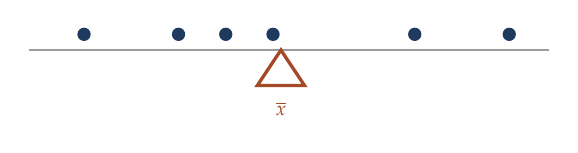
\begin{tikzpicture}[scale=1.0]
\draw[grau!60, line width=0.9pt] (-0.3,0) -- (6.3,0);
\foreach \x in {0.4, 1.6, 2.2, 2.8, 4.6, 5.8} \fill[tief] (\x,0.2) circle (2.4pt);
\draw[akzent, line width=1.2pt] (2.9,0) -- (2.6,-0.45) -- (3.2,-0.45) -- cycle;
\node[font=\scriptsize, color=akzent] at (2.9,-0.75) {$\MW$};
\end{tikzpicture}
\end{center}
\end{merksatz}

\begin{merksatz}
\boxtitel{Satz 2.4 --- Der Mittelwert minimiert die quadratischen Abstände}
Für jede reelle Zahl $a$ gilt
\[ \sum_{i=1}^n (x_i - a)^2 \;=\; \sum_{i=1}^n (x_i - \MW)^2 \;+\; n\,(\MW - a)^2 . \]
Insbesondere wird die linke Seite genau für $a = \MW$ am kleinsten.

\schritt{Beweis}
Der Kunstgriff ist, eine Null einzufügen: $x_i - a = (x_i - \MW) + (\MW - a)$.

\begin{align*}
\sum_i (x_i-a)^2 &= \sum_i \bigl[(x_i-\MW) + (\MW-a)\bigr]^2\\
&= \sum_i \Bigl[(x_i-\MW)^2 + 2(x_i-\MW)(\MW-a) + (\MW-a)^2\Bigr]\\
&= \sum_i (x_i-\MW)^2 \;+\; 2(\MW-a)\underbrace{\sum_i (x_i-\MW)}_{= 0 \text{ nach Satz 2.3}} \;+\; \sum_i (\MW-a)^2\\
&= \sum_i (x_i-\MW)^2 \;+\; 0 \;+\; n(\MW-a)^2 .
\end{align*}

\schritt{Der Schluss}
Der erste Summand hängt nicht von $a$ ab. Der zweite ist $\ge 0$ und genau dann null, wenn $a = \MW$. $\blacksquare$

\begin{center}
\begin{minipage}{0.88\textwidth}
\kursiv{Dieser Satz ist der Grund, warum der Mittelwert überall dort auftaucht, wo mit Quadraten gearbeitet wird --- bei der Varianz, bei der Regression, bei der Methode der kleinsten Quadrate. Er ist \kursiv{die} Zahl, die quadratische Abweichungen minimiert. Kapitel~10 baut die gesamte Regression darauf auf.}
\end{minipage}
\end{center}
\end{merksatz}

\section{Median, Quantile, Modus}

\begin{definition}
\boxtitelm{Definition 2.5 --- Median}
Seien die Daten aufsteigend sortiert: $x_{(1)} \le x_{(2)} \le \cdots \le x_{(n)}$. Dann ist
\[ \Med = \begin{cases}
x_{\left(\frac{n+1}{2}\right)}, & n \text{ ungerade},\\[6pt]
\dfrac{1}{2}\left(x_{\left(\frac{n}{2}\right)} + x_{\left(\frac{n}{2}+1\right)}\right), & n \text{ gerade}.
\end{cases} \]
\end{definition}

\begin{warnung}
\boxtitelr{Bei geradem $n$ verlässt man die Ordinalskala}
Für ungerades $n$ ist der Median eine der beobachteten Ausprägungen --- er ist rein durch die Rangfolge bestimmt und deshalb bei ordinalen Daten unbedenklich.

Für gerades $n$ wird gemittelt, und damit kommt die Abstandsannahme durch die Hintertür wieder herein. Streng genommen ist der Median ordinaler Daten bei geradem $n$ nicht eindeutig; man müsste jeden Wert zwischen den beiden mittleren zulassen.

\begin{center}
\begin{minipage}{0.88\textwidth}
\kursiv{In der Praxis mittelt man trotzdem. Wer es genau nehmen will, gibt bei ordinalen Daten und geradem $n$ beide mittleren Werte an --- etwa \enquote{Median zwischen 4 und 5}.}
\end{minipage}
\end{center}
\end{warnung}

\begin{merksatz}
\boxtitel{Satz 2.6 --- Der Median minimiert die absoluten Abstände}
Für ungerades $n$ wird
\[ \sum_{i=1}^n |x_i - a| \]
für $a = \Med$ am kleinsten.

\schritt{Beweis --- durch Verschieben}
Sei $a$ irgendeine Zahl und betrachten wir, was geschieht, wenn wir $a$ um ein kleines Stück $\varepsilon > 0$ nach rechts verschieben.

Für jeden Datenpunkt $x_i > a$ verringert sich $|x_i - a|$ um $\varepsilon$. Für jeden mit $x_i < a$ vergrößert er sich um $\varepsilon$.

Sei $L$ die Anzahl der Punkte links von $a$ und $R$ die Anzahl rechts. Die Gesamtänderung beträgt
\[ \varepsilon\,(L - R) . \]

\schritt{Die Folgerung}
\begin{center}
\renewcommand{\arraystretch}{1.5}
\begin{tabular}{@{}P{2.4cm}P{3.0cm}P{2.6cm}@{}}
\toprule
\textbf{Lage} & \textbf{Änderung} & \\
\midrule
$L < R$ & $\varepsilon(L-R) < 0$ & nach rechts gehen hilft\\
$L > R$ & $> 0$ & nach links gehen hilft\\
$L = R$ & $= 0$ & \textcolor{gruen}{Minimum erreicht}\\
\bottomrule
\end{tabular}
\end{center}

Die Summe wird also dort am kleinsten, wo links und rechts gleich viele Punkte liegen --- und das ist bei ungeradem $n$ genau der mittlere Wert, also der Median. $\blacksquare$

\begin{center}
\begin{minipage}{0.88\textwidth}
\kursiv{Damit haben Mittelwert und Median jeweils eine eigene Rechtfertigung. Der eine minimiert quadratische, der andere absolute Abweichungen. Welche Wahl richtig ist, hängt davon ab, wie man große Abweichungen gewichten will --- und das ist eine Sachentscheidung, keine mathematische.}
\end{minipage}
\end{center}
\end{merksatz}

\begin{definition}
\boxtitelm{Definition 2.7 --- Quantile}
Für $0 < p < 1$ ist das \Begriff{$p$-Quantil} $Q_p$ ein Wert, unterhalb dessen mindestens der Anteil $p$ der Daten liegt und oberhalb dessen mindestens der Anteil $1-p$ liegt.

Besondere Namen tragen
\begin{center}
\renewcommand{\arraystretch}{1.45}
\begin{tabular}{@{}P{2.4cm}P{2.0cm}P{3.4cm}@{}}
\toprule
$Q_{0{,}25}$ & unteres Quartil & auch $Q_1$\\
$Q_{0{,}50}$ & Median & auch $Q_2$\\
$Q_{0{,}75}$ & oberes Quartil & auch $Q_3$\\
\bottomrule
\end{tabular}
\end{center}
\end{definition}

\begin{warnung}
\boxtitelr{Es gibt neun gängige Definitionen --- und sie liefern verschiedene Zahlen}
Die Definition oben lässt bei kleinen Stichproben offen, welcher Wert genau zu nehmen ist. Verschiedene Statistikprogramme füllen diese Lücke verschieden aus; die Programmiersprache R kennt neun Verfahren.

\schritt{Was dieser Band tut}
Wir benutzen durchgehend die anschaulichste Konvention:

\begin{center}
\begin{minipage}{0.9\textwidth}
\textbf{Das untere Quartil ist der Median der unteren Hälfte, das obere der Median der oberen Hälfte. Bei ungeradem $n$ gehört der Median selbst zu keiner der beiden Hälften.}
\end{minipage}
\end{center}

\begin{center}
\begin{minipage}{0.88\textwidth}
\kursiv{Bei $n = 6$ oder $n = 100$ spielt die Wahl kaum eine Rolle; bei $n = 7$ kann sie sichtbar werden. Wichtig ist nur, dass man sie \kursiv{nennt} --- ein Quartil ohne Angabe der Konvention ist bei kleinen Stichproben keine reproduzierbare Zahl.}
\end{minipage}
\end{center}
\end{warnung}

\begin{definition}
\boxtitelm{Definition 2.8 --- Modus}
Der \Begriff{Modus} ist die häufigste Ausprägung. Er kann mehrdeutig sein und ist die einzige Lagekennzahl, die auch bei nominalen Merkmalen sinnvoll ist.
\end{definition}

\section{Robustheit}

\begin{merksatz}
\boxtitel{Ein Ausreißer, und was er anrichtet}
Nehmen wir die Mobilisationszeiten der Gruppe B: $18, 15, 21, 17, 23, 14$.

\begin{center}
\renewcommand{\arraystretch}{1.48}
\begin{tabular}{@{}P{3.0cm}P{2.2cm}P{2.6cm}@{}}
\toprule
& \textbf{Original} & \textbf{mit Tippfehler}\\
\midrule
Daten & $\ldots,\ 23,\ 14$ & $\ldots,\ 230,\ 14$\\
Mittelwert & $18{,}0$ & \textcolor{akzent}{$\mathbf{52{,}5}$}\\
Median & $17{,}5$ & \textcolor{gruen}{$\mathbf{17{,}5}$}\\
\bottomrule
\end{tabular}
\end{center}

\schritt{Die Rechnung}
Original: $\frac{18+15+21+17+23+14}{6} = \frac{108}{6} = 18$.

Mit Tippfehler: $\frac{108 - 23 + 230}{6} = \frac{315}{6} = 52{,}5$.

Der Median: sortiert $14, 15, 17, 18, 21, 230$ --- die beiden mittleren sind weiterhin $17$ und $18$.

\begin{center}
\begin{minipage}{0.88\textwidth}
\kursiv{Ein einziger falsch eingegebener Wert verdreifacht den Mittelwert und lässt den Median unberührt. In der Datenprüfung ist das ein Werkzeug: Weichen Mittelwert und Median stark voneinander ab, lohnt ein Blick auf die Rohdaten.}
\end{minipage}
\end{center}
\end{merksatz}

\begin{definition}
\boxtitelm{Definition 2.9 --- Bruchpunkt}
Der \Begriff{Bruchpunkt} einer Kennzahl ist der größte Anteil der Daten, den man beliebig verändern kann, ohne dass die Kennzahl beliebig groß oder klein wird.
\end{definition}

\begin{merksatz}
\boxtitel{Die Bruchpunkte im Vergleich}
\begin{center}
\renewcommand{\arraystretch}{1.48}
\begin{tabular}{@{}P{3.2cm}P{2.0cm}P{2.8cm}@{}}
\toprule
\textbf{Kennzahl} & \textbf{Bruch\-punkt} & \\
\midrule
Mittelwert & $0$ & \textcolor{akzent}{ein Wert genügt}\\
Spannweite & $0$ & \textcolor{akzent}{ein Wert genügt}\\
Standard\-abweichung & $0$ & \textcolor{akzent}{ein Wert genügt}\\
Quartilsabstand & $25\,\%$ & \textcolor{gruen}{robust}\\
\textbf{Median} & $\mathbf{50\,\%}$ & \textcolor{gruen}{\textbf{höchstmöglich}}\\
\bottomrule
\end{tabular}
\end{center}

\schritt{Warum $50\,\%$ das Maximum ist}
Könnte man mehr als die Hälfte der Daten beliebig setzen, so könnte man sie alle auf denselben, beliebig großen Wert legen --- und da sie dann die Mehrheit bildeten, müsste jede sinnvolle Lagekennzahl mitwandern. Mehr als $50\,\%$ Bruchpunkt ist also unmöglich.

\schritt{Warum der Mittelwert Bruchpunkt $0$ hat}
Bei $n$ Werten und einem veränderten: Setzt man $x_1 \to \infty$, so geht $\MW \to \infty$. Der Anteil $1/n$ geht für wachsendes $n$ gegen null --- daher der Bruchpunkt $0$.
\end{merksatz}

\section{Streuungsmaße}

\begin{definition}
\boxtitelm{Definition 2.10 --- die vier Streuungsmaße}
\begin{center}
\renewcommand{\arraystretch}{1.6}
\begin{tabular}{@{}P{3.6cm}P{4.8cm}@{}}
\toprule
Spannweite & $R = x_{(n)} - x_{(1)}$\\
Quartilsabstand & $\mathrm{IQR} = Q_3 - Q_1$\\
Stichprobenvarianz & $s^2 = \dfrac{1}{n-1}\displaystyle\sum_{i=1}^n (x_i - \MW)^2$\\
Standardabweichung & $s = \sqrt{s^2}$\\
\bottomrule
\end{tabular}
\end{center}
\end{definition}

\begin{warnung}
\boxtitelr{Warum $n-1$ und nicht $n$? --- vertagt, nicht verschwiegen}
Die Division durch $n-1$ statt durch $n$ ist die auffälligste Stelle der Formel und wird in Lehrbüchern gern mit \enquote{Freiheitsgrade} abgetan.

Eine ehrliche Begründung braucht den Erwartungswertbegriff und gehört daher in Kapitel~5, wo sie vollständig geführt wird. Hier nur die Vorschau:

\begin{center}
\begin{minipage}{0.9\textwidth}
Teilte man durch $n$, so wäre das Ergebnis \kursiv{im Mittel zu klein} --- und zwar systematisch, nicht zufällig. Der Grund: Die Abweichungen werden vom \kursiv{geschätzten} Mittelwert gemessen, und dieser liegt nach Satz 2.4 näher an den Daten als der wahre. Der Faktor $\frac{n}{n-1}$ korrigiert genau diesen Fehler.
\end{minipage}
\end{center}

\begin{center}
\begin{minipage}{0.88\textwidth}
\kursiv{Für rein beschreibende Zwecke --- wenn man nur die vorliegenden Daten zusammenfasst und nichts über eine Grundgesamtheit aussagen will --- wäre $n$ richtiger. Da man das fast nie tut, hat sich $n-1$ durchgesetzt.}
\end{minipage}
\end{center}
\end{warnung}

\begin{merksatz}
\boxtitel{Satz 2.11 --- der Verschiebungssatz}
\[ \sum_{i=1}^n (x_i - \MW)^2 \;=\; \sum_{i=1}^n x_i^2 \;-\; n\,\MW^2 . \]

\schritt{Beweis}
\begin{align*}
\sum_i (x_i - \MW)^2 &= \sum_i \bigl(x_i^2 - 2x_i\MW + \MW^2\bigr)\\
&= \sum_i x_i^2 \;-\; 2\MW\sum_i x_i \;+\; n\MW^2\\
&= \sum_i x_i^2 \;-\; 2\MW \cdot n\MW \;+\; n\MW^2 \qquad \Bigl(\text{denn } \sum_i x_i = n\MW\Bigr)\\
&= \sum_i x_i^2 - 2n\MW^2 + n\MW^2 \;=\; \sum_i x_i^2 - n\MW^2 . \qquad \blacksquare
\end{align*}

\schritt{Wozu das gut ist}
Die linke Seite verlangt zwei Durchgänge durch die Daten: erst den Mittelwert bestimmen, dann die Abweichungen. Die rechte Seite kommt mit einem aus --- man summiert gleichzeitig $x_i$ und $x_i^2$.

\begin{center}
\begin{minipage}{0.88\textwidth}
\kursiv{\textbf{Achtung bei der numerischen Anwendung.} Sind die Werte groß und die Streuung klein --- etwa Körpergrößen in Millimetern ---, so werden auf der rechten Seite zwei fast gleich große Zahlen voneinander abgezogen, und es kommt zur Auslöschung. Band 5 der Reihe behandelt das; für Handrechnungen ist die Formel unbedenklich.}
\end{minipage}
\end{center}
\end{merksatz}

\begin{merksatz}
\boxtitel{Die MOBIL-Daten, vollständig durchgerechnet}
\schritt{Gruppe B --- die einfacheren Zahlen}
Daten: $18, 15, 21, 17, 23, 14$, also $n = 6$.

\textbf{Summe und Mittelwert:}
\[ \sum x_i = 18+15+21+17+23+14 = 108, \qquad \MW_B = \frac{108}{6} = 18{,}0 . \]

\textbf{Quadratsumme:}
\[ \sum x_i^2 = 324 + 225 + 441 + 289 + 529 + 196 = 2004 . \]

\textbf{Verschiebungssatz:}
\[ \sum (x_i - \MW)^2 = 2004 - 6 \cdot 18^2 = 2004 - 6 \cdot 324 = 2004 - 1944 = 60 . \]

\textbf{Varianz und Standardabweichung:}
\[ s_B^2 = \frac{60}{6-1} = \frac{60}{5} = 12{,}0, \qquad s_B = \sqrt{12} \approx 3{,}46 . \]

\textbf{Probe durch direktes Nachrechnen:}
\begin{center}
{\small
\renewcommand{\arraystretch}{1.35}
\begin{tabular}{@{}P{1.2cm}P{1.6cm}P{1.8cm}@{}}
\toprule
$x_i$ & $x_i - 18$ & $(x_i-18)^2$\\
\midrule
$18$ & $0$ & $0$\\
$15$ & $-3$ & $9$\\
$21$ & $3$ & $9$\\
$17$ & $-1$ & $1$\\
$23$ & $5$ & $25$\\
$14$ & $-4$ & $16$\\
\midrule
& $\mathbf{0}$ & $\mathbf{60}$\\
\bottomrule
\end{tabular}}
\end{center}
Die mittlere Spalte summiert sich zu null --- das ist Satz 2.3. \checkmark\ Die rechte zu $60$. \checkmark

\schritt{Gruppe A}
Daten: $26, 19, 31, 24, 35, 22$.
\[ \sum x_i = 157, \qquad \MW_A = \frac{157}{6} \approx 26{,}17 . \]
\[ \sum x_i^2 = 676+361+961+576+1225+484 = 4283 . \]
\[ \sum (x_i-\MW)^2 = 4283 - 6\cdot\Bigl(\tfrac{157}{6}\Bigr)^{\!2} = 4283 - \frac{24649}{6} \approx 174{,}83 . \]
\[ s_A^2 = \frac{174{,}83}{5} = 34{,}97, \qquad s_A \approx 5{,}91 . \]

\schritt{Median und Quartile}
\begin{center}
{\small
\renewcommand{\arraystretch}{1.42}
\begin{tabular}{@{}P{1.6cm}P{3.4cm}P{1.4cm}P{1.4cm}@{}}
\toprule
& \textbf{sortiert} & \textbf{Median} & \textbf{IQR}\\
\midrule
A & $19, 22, 24, 26, 31, 35$ & $25{,}0$ & $9$\\
B & $14, 15, 17, 18, 21, 23$ & $17{,}5$ & $6$\\
\bottomrule
\end{tabular}}
\end{center}

Für A: untere Hälfte $19,22,24$, Median davon $Q_1 = 22$; obere Hälfte $26,31,35$, also $Q_3 = 31$. IQR $= 9$.\\
Für B: $Q_1 = 15$, $Q_3 = 21$, IQR $= 6$.

\schritt{Die Zusammenfassung}
\begin{center}
{\small
\renewcommand{\arraystretch}{1.45}
\begin{tabular}{@{}P{2.6cm}P{2.2cm}P{2.2cm}@{}}
\toprule
& \textbf{Gruppe A} & \textbf{Gruppe B}\\
\midrule
$n$ & $6$ & $6$\\
Mittelwert & $26{,}2$ & $18{,}0$\\
Standardabw. & $5{,}9$ & $3{,}5$\\
Median & $25{,}0$ & $17{,}5$\\
IQR & $9$ & $6$\\
Spannweite & $16$ & $9$\\
\bottomrule
\end{tabular}}
\end{center}

\begin{center}
\begin{minipage}{0.88\textwidth}
\kursiv{Gruppe B mobilisiert nicht nur früher, sondern auch \kursiv{einheitlicher} --- beide Streuungsmaße sind kleiner. Das ist eine eigene Beobachtung und oft die klinisch interessantere: Ein Verfahren, das bei allen ähnlich wirkt, ist planbarer als eines mit gleichem Mittelwert und großer Streuung.}
\end{minipage}
\end{center}
\end{merksatz}

\begin{definition}
\boxtitelm{Definition 2.12 --- Variationskoeffizient und Standardisierung}
\begin{itemize}[leftmargin=1.4em, itemsep=4pt]
\item Der \Begriff{Variationskoeffizient} ist $v = s/\MW$ --- die Streuung im Verhältnis zur Größenordnung. Er ist nur bei verhältnisskalierten Merkmalen mit positivem Mittelwert sinnvoll.
\item Der \Begriff{$z$-Wert} einer Beobachtung ist
\[ z_i = \frac{x_i - \MW}{s} . \]
\end{itemize}
\end{definition}

\begin{merksatz}
\boxtitel{Was die Standardisierung leistet}
Die $z$-Werte haben stets Mittelwert $0$ und Standardabweichung $1$ --- unabhängig von der ursprünglichen Einheit.

\schritt{Ein Beispiel}
Die Person mit ID 5 hat $\mathrm{MOB} = 35$, in Gruppe A. Ihr $z$-Wert:
\[ z = \frac{35 - 26{,}17}{5{,}91} \approx 1{,}49 . \]
Sie liegt also etwa anderthalb Standardabweichungen über dem Gruppenmittel.

\begin{center}
\begin{minipage}{0.88\textwidth}
\kursiv{Der $z$-Wert macht Größen vergleichbar, die in verschiedenen Einheiten gemessen sind --- Mobilisationszeit und Operationsdauer etwa. Er beantwortet nicht die Frage, ob ein Wert ungewöhnlich \kursiv{ist}: Dafür bräuchte man eine Verteilungsannahme, und die liefert erst Kapitel~4.}
\end{minipage}
\end{center}
\end{merksatz}

\section{Der Boxplot}

\begin{merksatz}
\boxtitel{Wie er aufgebaut ist}
\begin{center}
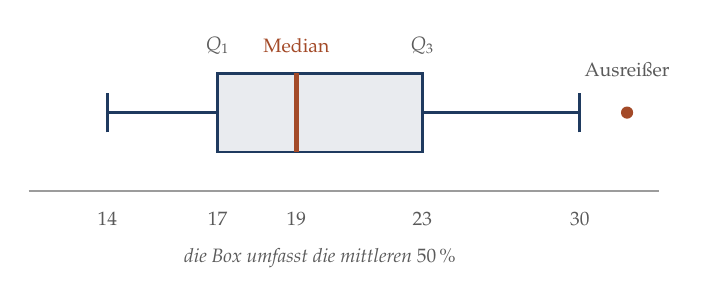
\begin{tikzpicture}[scale=1.0]
\draw[grau!60, line width=0.7pt] (-0.4,0) -- (7.6,0);
\foreach \x/\lab in {0.6/14, 2.0/17, 3.0/19, 4.6/23, 6.6/30}
  \node[font=\scriptsize, color=grau] at (\x,-0.35) {\lab};
% Box
\draw[tief, line width=1.0pt, fill=tief!10] (2.0,0.5) rectangle (4.6,1.5);
\draw[akzent, line width=1.6pt] (3.0,0.5) -- (3.0,1.5);
\draw[tief, line width=1.0pt] (2.0,1.0) -- (0.6,1.0);
\draw[tief, line width=1.0pt] (4.6,1.0) -- (6.6,1.0);
\draw[tief, line width=1.0pt] (0.6,0.75) -- (0.6,1.25);
\draw[tief, line width=1.0pt] (6.6,0.75) -- (6.6,1.25);
\fill[akzent] (7.2,1.0) circle (2.2pt);
\node[font=\scriptsize, color=grau] at (2.0,1.85) {$Q_1$};
\node[font=\scriptsize, color=akzent] at (3.0,1.85) {Median};
\node[font=\scriptsize, color=grau] at (4.6,1.85) {$Q_3$};
\node[font=\scriptsize, color=grau] at (7.2,1.55) {Ausreißer};
\node[font=\scriptsize\itshape, color=grau] at (3.3,-0.85) {die Box umfasst die mittleren $50\,\%$};
\end{tikzpicture}
\end{center}

\begin{center}
\renewcommand{\arraystretch}{1.5}
\begin{tabular}{@{}P{2.4cm}P{6.2cm}@{}}
\toprule
\textbf{Box} & von $Q_1$ bis $Q_3$; die Breite ist der IQR\\
\textbf{Strich} & der Median\\
\textbf{Schnurrhaare} & bis zum weitesten Wert innerhalb von $1{,}5 \cdot \mathrm{IQR}$ ab der Box\\
\textbf{Punkte} & alles darüber hinaus, einzeln eingezeichnet\\
\bottomrule
\end{tabular}
\end{center}
\end{merksatz}

\begin{warnung}
\boxtitelr{Die $1{,}5$ ist eine Konvention, keine Entdeckung}
\Person{John Tukey} wählte den Faktor $1{,}5$, weil er bei normalverteilten Daten etwa $0{,}7\,\%$ der Beobachtungen als Ausreißer markiert --- selten genug, um auffällig zu sein, häufig genug, um nicht leer auszugehen.

\begin{center}
\begin{minipage}{0.9\textwidth}
\textbf{Ein Punkt im Boxplot ist daher kein Messfehler und kein Grund zum Ausschluss.} Er ist ein Hinweis, hinzusehen --- nicht mehr.
\end{minipage}
\end{center}

Bei schiefen Verteilungen --- und Zeitdauern sind fast immer rechtsschief --- markiert die Regel systematisch zu viele Punkte am oberen Rand. Das ist kein Befund über die Daten, sondern über die Regel.
\end{warnung}

\section{Das Anscombe-Quartett}

Jetzt der wichtigste Warnkasten dieses Kapitels.

\begin{merksatz}
\boxtitel{Vier Datensätze, elf Zahlenpaare, identische Kennzahlen}
\Person{Francis Anscombe} veröffentlichte 1973 vier Datensätze mit je elf Punkten.

\begin{center}
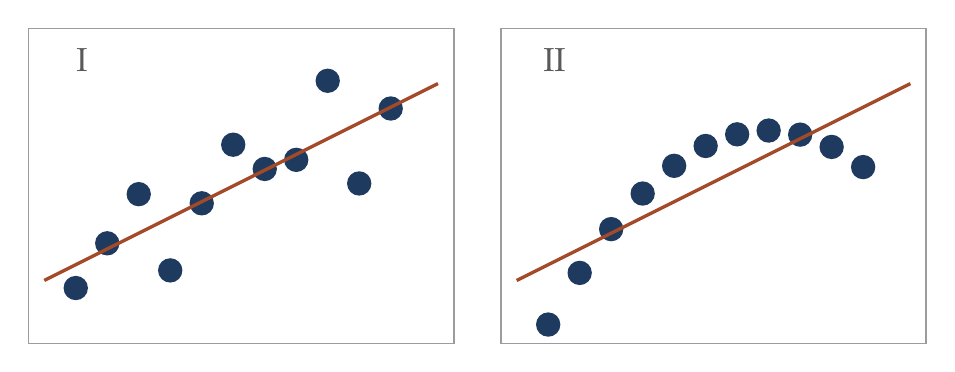
\begin{tikzpicture}[scale=0.40]
\def\axes{\draw[grau!60, line width=0.6pt] (2.5,2.5) rectangle (20,13);}
% I
\begin{scope}[xshift=0cm]
\draw[grau!60, line width=0.6pt] (2.5,2.5) rectangle (16,12.5);
\foreach \x/\y in {10/8.04, 8/6.95, 13/7.58, 9/8.81, 11/8.33, 14/9.96, 6/7.24, 4/4.26, 12/10.84, 7/4.82, 5/5.68}
  \fill[tief] (\x,\y) circle (11pt);
\draw[akzent, line width=1.2pt] (3,4.5) -- (15.5,10.75);
\node[font=\large, color=grau] at (4.2,11.5) {I};
\end{scope}
% II
\begin{scope}[xshift=15cm]
\draw[grau!60, line width=0.6pt] (2.5,2.5) rectangle (16,12.5);
\foreach \x/\y in {10/9.14, 8/8.14, 13/8.74, 9/8.77, 11/9.26, 14/8.10, 6/6.13, 4/3.10, 12/9.13, 7/7.26, 5/4.74}
  \fill[tief] (\x,\y) circle (11pt);
\draw[akzent, line width=1.2pt] (3,4.5) -- (15.5,10.75);
\node[font=\large, color=grau] at (4.2,11.5) {II};
\end{scope}
\end{tikzpicture}

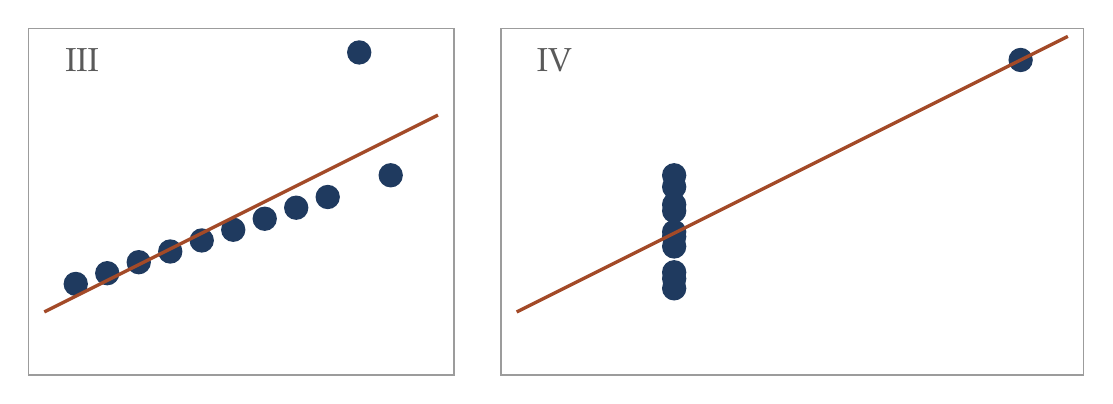
\begin{tikzpicture}[scale=0.40]
% III
\begin{scope}[xshift=0cm]
\draw[grau!60, line width=0.6pt] (2.5,2.5) rectangle (16,13.5);
\foreach \x/\y in {10/7.46, 8/6.77, 13/12.74, 9/7.11, 11/7.81, 14/8.84, 6/6.08, 4/5.39, 12/8.15, 7/6.42, 5/5.73}
  \fill[tief] (\x,\y) circle (11pt);
\draw[akzent, line width=1.2pt] (3,4.5) -- (15.5,10.75);
\node[font=\large, color=grau] at (4.2,12.5) {III};
\end{scope}
% IV
\begin{scope}[xshift=15cm]
\draw[grau!60, line width=0.6pt] (2.5,2.5) rectangle (21,13.5);
\foreach \y in {6.58, 5.76, 7.71, 8.84, 8.47, 7.04, 5.25, 5.56, 7.91, 6.89}
  \fill[tief] (8,\y) circle (11pt);
\fill[tief] (19,12.50) circle (11pt);
\draw[akzent, line width=1.2pt] (3,4.5) -- (20.5,13.25);
\node[font=\large, color=grau] at (4.2,12.5) {IV};
\end{scope}
\end{tikzpicture}
\end{center}

\schritt{Die Kennzahlen --- für alle vier gleich}
\begin{center}
{\small
\renewcommand{\arraystretch}{1.42}
\begin{tabular}{@{}P{3.6cm}P{2.6cm}@{}}
\toprule
\textbf{Kennzahl} & \textbf{Wert}\\
\midrule
Mittelwert von $x$ & $9{,}0$\\
Varianz von $x$ & $11{,}0$\\
Mittelwert von $y$ & $7{,}50$\\
Varianz von $y$ & $4{,}12$\\
Korrelation & $0{,}816$\\
Regressionsgerade & $y = 3{,}00 + 0{,}500\,x$\\
\bottomrule
\end{tabular}}
\end{center}

\schritt{Was die Bilder zeigen}
\begin{center}
\renewcommand{\arraystretch}{1.5}
\begin{tabular}{@{}P{1.2cm}P{7.2cm}@{}}
\toprule
I & Ein Zusammenhang, wie man ihn erwartet. Hier ist alles in Ordnung.\\
II & Ein deutlich \kursiv{gekrümmter} Zusammenhang. Eine Gerade ist das falsche Modell.\\
III & Ein exakter linearer Zusammenhang plus \kursiv{ein} Ausreißer, der die Gerade verzieht.\\
IV & Alle $x$ bis auf eines gleich. Die Gerade wird von einem einzigen Punkt bestimmt.\\
\bottomrule
\end{tabular}
\end{center}
\end{merksatz}

\begin{warnung}
\boxtitelr{Die Lehre}
\begin{center}
\begin{minipage}{0.9\textwidth}
\textbf{Kennzahlen ersetzen das Bild nicht. Sie fassen zusammen, und Zusammenfassen heißt Weglassen --- man weiß nur nicht immer, was.}
\end{minipage}
\end{center}

Im vierten Datensatz ist die Lage besonders bedenklich: Entfernt man den einen rechten Punkt, so ist die Steigung nicht mehr bestimmbar, denn alle übrigen $x$ sind gleich. Die Regressionsgerade beruht vollständig auf einer einzigen Beobachtung --- und keine der sechs Kennzahlen verrät das.

\begin{center}
\begin{minipage}{0.88\textwidth}
\kursiv{Anscombe schrieb dazu den Satz, der das Anliegen seines Aufsatzes zusammenfasst: Ein Rechner solle uns nicht vom Hinsehen abhalten, sondern es ermöglichen. Das war 1973 eine Forderung; heute ist es eine Selbstverständlichkeit, an die man sich trotzdem erinnern muss.}
\end{minipage}
\end{center}
\end{warnung}

\begin{technik}
\boxtitelm{Zur Kontrolle in R}
\begin{center}
\begin{minipage}{0.82\textwidth}
\code{mobB <- c(18, 15, 21, 17, 23, 14)}\\
\code{mean(mobB); sd(mobB); median(mobB)}\\
\code{quantile(mobB, c(.25,.75), type = 2)}
\end{minipage}
\end{center}

Das Argument \code{type = 2} wählt die Konvention dieses Bandes --- Median der Hälften. Ohne Angabe benutzt R \code{type = 7} und liefert $Q_1 = 15{,}5$ statt $15$.
\end{technik}

\section{Übungsaufgaben}

\begin{aufgabe}
\boxtitel{Aufgabe 2.1 --- Alle Kennzahlen für das Alter}
Bestimmen Sie für das Merkmal \code{ALTER} aller zwölf Beobachtungen Mittelwert, Median, Quartile, Spannweite, Varianz und Standardabweichung.

\loesung
\schritt{Schritt 1 --- Die Daten}
\[ 68,\ 74,\ 61,\ 79,\ 70,\ 65,\ 72,\ 66,\ 81,\ 69,\ 75,\ 63 \]
Sortiert:
\[ 61,\ 63,\ 65,\ 66,\ 68,\ 69,\ 70,\ 72,\ 74,\ 75,\ 79,\ 81 \]

\schritt{Schritt 2 --- Mittelwert}
\begin{align*}
\sum x_i &= 61+63+65+66+68+69+70+72+74+75+79+81
\end{align*}
Wir addieren paarweise von außen:
\[ 61+81 = 142, \quad 63+79 = 142, \quad 65+75 = 140, \]
\[ 66+74 = 140, \quad 68+72 = 140, \quad 69+70 = 139 \]
\[ \sum x_i = 142+142+140+140+140+139 = 843 \]
\[ \MW = \frac{843}{12} = 70{,}25 \]

\schritt{Schritt 3 --- Median und Quartile}
$n = 12$ ist gerade; die mittleren beiden sind der sechste und siebte Wert: $69$ und $70$.
\[ \Med = \frac{69+70}{2} = 69{,}5 \]

Untere Hälfte (sechs Werte): $61,63,65,66,68,69$. Ihr Median:
\[ Q_1 = \frac{65+66}{2} = 65{,}5 \]
Obere Hälfte: $70,72,74,75,79,81$.
\[ Q_3 = \frac{74+75}{2} = 74{,}5 \]
\[ \mathrm{IQR} = 74{,}5 - 65{,}5 = 9{,}0 \]

\schritt{Schritt 4 --- Spannweite}
\[ R = 81 - 61 = 20 \]

\schritt{Schritt 5 --- Varianz über den Verschiebungssatz}
\begin{align*}
\sum x_i^2 &= 3721+3969+4225+4356+4624+4761\\
&\quad + 4900+5184+5476+5625+6241+6561
\end{align*}
Wir addieren in Blöcken:
\[ 3721+3969 = 7690, \quad 4225+4356 = 8581, \quad 4624+4761 = 9385 \]
\[ 4900+5184 = 10084, \quad 5476+5625 = 11101, \quad 6241+6561 = 12802 \]
\[ \sum x_i^2 = 7690+8581+9385+10084+11101+12802 = 59643 \]

\[ n\MW^2 = 12 \cdot 70{,}25^2 = 12 \cdot 4935{,}0625 = 59220{,}75 \]
\[ \sum(x_i-\MW)^2 = 59643 - 59220{,}75 = 422{,}25 \]
\[ s^2 = \frac{422{,}25}{11} = 38{,}39, \qquad s = \sqrt{38{,}39} \approx 6{,}20 \]

\schritt{Schritt 6 --- Die Zusammenfassung}
\begin{center}
\renewcommand{\arraystretch}{1.42}
\begin{tabular}{@{}P{2.6cm}P{1.8cm}P{2.6cm}P{1.8cm}@{}}
\toprule
Mittelwert & $70{,}25$ & Spannweite & $20$\\
Median & $69{,}5$ & Varianz & $38{,}39$\\
$Q_1$, $Q_3$ & $65{,}5$; $74{,}5$ & Standardabw. & $6{,}20$\\
\bottomrule
\end{tabular}
\end{center}

\schritt{Probe}
Mittelwert und Median liegen dicht beieinander ($70{,}25$ gegen $69{,}5$) --- ein Hinweis auf eine annähernd symmetrische Verteilung ohne Ausreißer. Dazu passt, dass die Spannweite mit $20$ etwa dem Dreifachen des IQR entspricht; bei starken Ausreißern wäre das Verhältnis größer.
\end{aufgabe}

\begin{aufgabe}
\boxtitel{Aufgabe 2.2 --- Was ein Umrechnen der Einheit bewirkt}
Die Mobilisationszeiten der Gruppe B sollen in Minuten statt Stunden angegeben werden. Wie ändern sich Mittelwert, Median, Standardabweichung, Varianz und Variationskoeffizient?

\loesung
\schritt{Schritt 1 --- Die Umformung benennen}
$y_i = 60\,x_i$, also von der Bauart $y = a x$ mit $a = 60$.

\schritt{Schritt 2 --- Der Mittelwert}
\[ \MW_y = \frac{1}{n}\sum_i 60 x_i = 60 \cdot \frac{1}{n}\sum_i x_i = 60\,\MW_x = 60 \cdot 18 = 1080 \ \text{min} . \]
Hier wurde die zweite Summenregel benutzt.

\schritt{Schritt 3 --- Der Median}
Der Median ist eine der Beobachtungen beziehungsweise das Mittel zweier Beobachtungen. Da die Umformung streng wachsend ist, bleibt die Rangfolge erhalten, und es werden dieselben Positionen genommen:
\[ \Med_y = 60 \cdot 17{,}5 = 1050 \ \text{min} . \]

\schritt{Schritt 4 --- Die Varianz}
\[ s_y^2 = \frac{1}{n-1}\sum_i (60x_i - 60\MW_x)^2 = \frac{1}{n-1}\sum_i 60^2 (x_i-\MW_x)^2 = 3600\,s_x^2 . \]
\[ s_y^2 = 3600 \cdot 12 = 43\,200 \ \text{min}^2 . \]

\schritt{Schritt 5 --- Die Standardabweichung}
\[ s_y = \sqrt{43\,200} = 60 \cdot \sqrt{12} \approx 207{,}8 \ \text{min} . \]

\schritt{Schritt 6 --- Der Variationskoeffizient}
\[ v_y = \frac{s_y}{\MW_y} = \frac{60\,s_x}{60\,\MW_x} = \frac{s_x}{\MW_x} = v_x . \]
\[ v = \frac{3{,}46}{18{,}0} = 0{,}192 \ \text{--- in beiden Einheiten}. \]

\schritt{Die Übersicht}
\begin{center}
{\small
\renewcommand{\arraystretch}{1.45}
\begin{tabular}{@{}P{3.4cm}P{2.0cm}P{2.6cm}@{}}
\toprule
\textbf{Kennzahl} & \textbf{Faktor} & \textbf{Wert (min)}\\
\midrule
Mittelwert & $60$ & $1080$\\
Median & $60$ & $1050$\\
Standard\-abweichung & $60$ & $207{,}8$\\
Varianz & $\mathbf{3600}$ & $43\,200$\\
\textbf{Variationskoeffizient} & $\mathbf{1}$ & \textcolor{gruen}{$\mathbf{0{,}192}$}\\
\bottomrule
\end{tabular}}
\end{center}

\schritt{Die Lehre}
Die Varianz ändert sich mit dem \kursiv{Quadrat} des Faktors --- sie trägt die Einheit \enquote{Minuten zum Quadrat}, was sich kaum deuten lässt. Genau deshalb gibt man die Standardabweichung an: Sie hat dieselbe Einheit wie die Daten.

Der Variationskoeffizient ist als einzige Kennzahl \kursiv{einheitenfrei} und deshalb der richtige Maßstab, wenn man die Streuung zweier verschieden gemessener Größen vergleichen will.
\end{aufgabe}

\begin{aufgabe}
\boxtitel{Aufgabe 2.3 --- Ein Datensatz zum Anscombe-Muster}
Konstruieren Sie zwei Datensätze mit je fünf Werten, die denselben Mittelwert und dieselbe Standardabweichung haben, aber offensichtlich verschieden sind.

\loesung
\schritt{Schritt 1 --- Was zu erfüllen ist}
Gesucht sind $x_1,\ldots,x_5$ und $y_1,\ldots,y_5$ mit gleicher Summe und gleicher Quadratsumme --- denn daraus folgen nach dem Verschiebungssatz gleicher Mittelwert und gleiche Varianz.

\schritt{Schritt 2 --- Ein Ansatz über Symmetrie}
Wir wählen beide Datensätze symmetrisch um $10$, so dass der Mittelwert automatisch $10$ ist:
\[ A: \ 6,\ 8,\ 10,\ 12,\ 14 \qquad B: \ 10-c,\ 10-d,\ 10,\ 10+d,\ 10+c \]

\schritt{Schritt 3 --- Die Bedingung an die Quadratsumme}
Für A:
\[ \sum (x_i - 10)^2 = 16 + 4 + 0 + 4 + 16 = 40 . \]
Für B:
\[ 2c^2 + 2d^2 = 40 \quad\Longrightarrow\quad c^2 + d^2 = 20 . \]

\schritt{Schritt 4 --- Eine Lösung suchen}
Wir brauchen ein Paar mit $c^2 + d^2 = 20$, das anders aussieht als $c=4$, $d=2$.

Nehmen wir $c = \sqrt{18} \approx 4{,}243$ und $d = \sqrt{2} \approx 1{,}414$: dann $18 + 2 = 20$. \checkmark

\[ B: \ 5{,}76;\ 8{,}59;\ 10;\ 11{,}41;\ 14{,}24 \]

Das ist zulässig, aber unschön. Schöner mit ganzen Zahlen: Es gibt keine ganzzahlige Lösung außer $(4,2)$ und $(2,4)$ --- die aber dieselbe Menge liefern. Wir weichen deshalb von der Symmetrie ab.

\schritt{Schritt 5 --- Ein ganzzahliges Beispiel}
\[ A: \ 6,\ 8,\ 10,\ 12,\ 14 \qquad B: \ 4,\ 11,\ 11,\ 11,\ 13 \]

\textbf{Probe für B:}
\[ \sum y_i = 4+11+11+11+13 = 50 \quad\Rightarrow\quad \MW_B = 10 \ \checkmark \]
\begin{center}
{\small
\renewcommand{\arraystretch}{1.32}
\begin{tabular}{@{}P{1.2cm}P{1.6cm}P{1.8cm}@{}}
\toprule
$y_i$ & $y_i - 10$ & $(y_i-10)^2$\\
\midrule
$4$ & $-6$ & $36$\\
$11$ & $1$ & $1$\\
$11$ & $1$ & $1$\\
$11$ & $1$ & $1$\\
$13$ & $3$ & $9$\\
\midrule
& $\mathbf{0}$ & $\mathbf{48}$\\
\bottomrule
\end{tabular}}
\end{center}

$48 \neq 40$. Die Quadratsummen stimmen noch nicht.

\schritt{Schritt 6 --- Nachjustieren}
Wir ersetzen die $13$ durch $12$ und gleichen die Summe mit einer $12$ statt einer $11$ aus:
\[ B: \ 4,\ 11,\ 11,\ 12,\ 12 \]
\[ \sum y_i = 4+11+11+12+12 = 50 \ \checkmark \]
\[ \sum (y_i-10)^2 = 36 + 1 + 1 + 4 + 4 = 46 . \]
Noch immer zu groß. Der Ausreißer $4$ trägt allein $36$ bei; wir müssen ihn abschwächen.

\[ B: \ 5,\ 10,\ 11,\ 12,\ 12 \]
\[ \sum = 50 \ \checkmark, \qquad \sum(y_i-10)^2 = 25+0+1+4+4 = 34 . \]
Jetzt zu klein. Zwischen $46$ und $34$ liegt $40$; wir probieren
\[ B: \ 5,\ 9,\ 11,\ 12,\ 13 \]
\[ \sum = 50 \ \checkmark, \qquad \sum(y_i-10)^2 = 25+1+1+4+9 = 40 . \quad \checkmark \]

\schritt{Schritt 7 --- Das Ergebnis}
\begin{center}
\renewcommand{\arraystretch}{1.45}
\begin{tabular}{@{}P{2.4cm}P{3.0cm}P{2.4cm}@{}}
\toprule
& \textbf{Daten} & \textbf{Median}\\
\midrule
A & $6, 8, 10, 12, 14$ & $10$\\
B & $5, 9, 11, 12, 13$ & $11$\\
\bottomrule
\end{tabular}
\end{center}
Beide: $\MW = 10$, $\sum(x-\MW)^2 = 40$, also $s^2 = 10$ und $s \approx 3{,}16$.

Die Datensätze unterscheiden sich dennoch deutlich: A ist symmetrisch, B ist linksschief --- der Median liegt über dem Mittelwert, und ein niedriger Wert zieht nach unten.

\schritt{Nachbemerkung zum Vorgehen}
Ich habe den Weg mit den Fehlversuchen stehen lassen. So arbeitet man tatsächlich: Man rät, rechnet nach, korrigiert in die richtige Richtung. Der Verschiebungssatz macht dabei jeden Versuch zu einer Sache von zwei Zeilen.
\end{aufgabe}

\begin{geschichte}
\boxtitelg{Quetelet und der Durchschnittsmensch}
Der Mittelwert war lange ein Werkzeug der Astronomie: Mehrere Messungen desselben Sterns wurden gemittelt, um den Messfehler zu verkleinern. Dahinter steht eine klare Vorstellung --- es gibt einen wahren Wert, und die Abweichungen sind Fehler.

\Person{Adolphe Quetelet} (1796--1874), belgischer Astronom und Statistiker, übertrug den Gedanken um 1835 auf den Menschen. Er mittelte Körpergrößen, Brustumfänge und Sterblichkeitsraten und prägte den Begriff des \kursiv{homme moyen} --- des Durchschnittsmenschen.

\begin{center}
\begin{minipage}{0.9\textwidth}
\kursiv{Der Übertragungsfehler steckt in der Deutung. Beim Stern ist die Abweichung ein Fehler; beim Menschen ist sie die Wirklichkeit. Quetelet verstand den Durchschnittsmenschen als das eigentlich Gemeinte und die Abweichungen als Störung --- eine Vorstellung, die später zur Rechtfertigung übler Dinge diente.}
\end{minipage}
\end{center}

\Person{Florence Nightingale} war von Quetelets Methoden begeistert und benutzte sie mit umgekehrtem Vorzeichen: Sie zeigte 1858 mit Sterblichkeitsstatistiken der Krimkriegslazarette, dass weit mehr Soldaten an Infektionen als an Verwundungen starben --- und erzwang damit hygienische Reformen. Ihre Diagramme gehören zu den frühesten Beispielen dafür, dass eine gute Darstellung eine Entscheidung herbeiführen kann.
\end{geschichte}

\begin{forschung}
\boxtitelp{Wie heute berichtet wird}
Die Frage, ob man \enquote{Mittelwert $\pm$ Standardabweichung} oder \enquote{Median [IQR]} angibt, ist keine Geschmacksfrage.

\begin{center}
{\small
\renewcommand{\arraystretch}{1.45}
\begin{tabular}{@{}P{3.0cm}P{5.4cm}@{}}
\toprule
\textbf{Mittelwert $\pm$ SD} & nur bei annähernd symmetrischen Verteilungen\\
\textbf{Median [IQR]} & bei schiefen Verteilungen, kleinen Stichproben, ordinalen Daten\\
\textbf{Beides} & wenn der Vergleich mit der Literatur es erfordert\\
\bottomrule
\end{tabular}}
\end{center}

Die CONSORT-Empfehlungen für die Berichterstattung randomisierter Studien --- 2010 aufgestellt und 2025 grundlegend überarbeitet --- verlangen, dass Streuungsmaße ausdrücklich benannt werden. Der Grund ist ein verbreiteter Fehler: Die Angabe \enquote{$18{,}0 \pm 3{,}5$} lässt offen, ob $3{,}5$ die Standardabweichung oder der Standardfehler ist. Beide unterscheiden sich um den Faktor $\sqrt{n}$ --- bei $n=60$ also um fast das Achtfache.

\begin{center}
\begin{minipage}{0.88\textwidth}
\kursiv{Kapitel~4 führt den Unterschied vollständig ein. Merken Sie sich vorerst: Die Standardabweichung beschreibt die \kursiv{Daten}, der Standardfehler die Genauigkeit des \kursiv{Mittelwerts}. Wer den Standardfehler angibt, weil die Balken kleiner aussehen, täuscht.}
\end{minipage}
\end{center}
\end{forschung}

\begin{merksatz}
\boxtitel{Was Sie jetzt können}
\begin{center}
\renewcommand{\arraystretch}{1.5}
\begin{tabular}{@{}P{3.0cm}P{5.6cm}@{}}
\toprule
\textbf{Satz 2.3} & Abweichungen vom Mittelwert summieren sich zu null\\
\textbf{Satz 2.4} & Der Mittelwert minimiert quadratische Abstände\\
\textbf{Satz 2.6} & Der Median minimiert absolute Abstände\\
\textbf{Satz 2.11} & Verschiebungssatz --- Varianz in einem Durchgang\\
\textbf{Bruchpunkte} & Mittelwert $0$, Median $50\,\%$\\
\textbf{Anscombe} & Kennzahlen ersetzen das Bild nicht\\
\bottomrule
\end{tabular}
\end{center}

\begin{center}
\begin{minipage}{0.88\textwidth}
\kursiv{Im nächsten Kapitel betrachten wir zwei Merkmale gleichzeitig --- und stoßen auf die verbreitetste Fehldeutung der gesamten Statistik.}
\end{minipage}
\end{center}
\end{merksatz}

\chapter{Zusammenhang}

\section{Zwei Merkmale gleichzeitig}

Bisher haben wir jedes Merkmal für sich betrachtet. Die interessanten Fragen betreffen aber fast immer Beziehungen: Hängt der Schmerz mit der Mobilisationszeit zusammen? Wirkt das Schema bei Älteren anders?

\begin{merksatz}
\boxtitel{Das Streudiagramm}
Die erste Antwort ist immer ein Bild. Man trägt jede Beobachtung als Punkt ein: waagerecht das eine Merkmal, senkrecht das andere.

\begin{center}
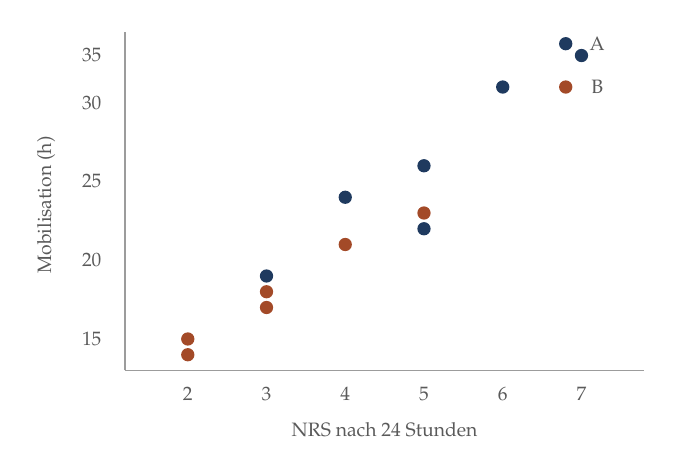
\begin{tikzpicture}[scale=1.0]
\draw[grau!60, line width=0.7pt] (0,0) -- (6.6,0);
\draw[grau!60, line width=0.7pt] (0,0) -- (0,4.3);
\foreach \x/\lab in {0.8/2, 1.8/3, 2.8/4, 3.8/5, 4.8/6, 5.8/7}
  \node[font=\scriptsize, color=grau] at (\x,-0.3) {\lab};
\foreach \y/\lab in {0.4/15, 1.4/20, 2.4/25, 3.4/30, 4.0/35}
  \node[font=\scriptsize, color=grau] at (-0.42,\y) {\lab};
% A-Gruppe (tief), B-Gruppe (akzent)
\fill[tief] (3.8,2.6) circle (2.4pt);
\fill[tief] (1.8,1.2) circle (2.4pt);
\fill[tief] (4.8,3.6) circle (2.4pt);
\fill[tief] (2.8,2.2) circle (2.4pt);
\fill[tief] (5.8,4.0) circle (2.4pt);
\fill[tief] (3.8,1.8) circle (2.4pt);
\fill[akzent] (1.8,1.0) circle (2.4pt);
\fill[akzent] (0.8,0.4) circle (2.4pt);
\fill[akzent] (2.8,1.6) circle (2.4pt);
\fill[akzent] (1.8,0.8) circle (2.4pt);
\fill[akzent] (3.8,2.0) circle (2.4pt);
\fill[akzent] (0.8,0.2) circle (2.4pt);
\node[font=\scriptsize, color=grau] at (3.3,-0.75) {NRS nach 24 Stunden};
\node[font=\scriptsize, color=grau, rotate=90] at (-1.0,2.1) {Mobilisation (h)};
\fill[tief] (5.6,4.15) circle (2.4pt);
\node[font=\scriptsize, color=grau] at (6.0,4.15) {A};
\fill[akzent] (5.6,3.6) circle (2.4pt);
\node[font=\scriptsize, color=grau] at (6.0,3.6) {B};
\end{tikzpicture}
\end{center}

\begin{center}
\begin{minipage}{0.88\textwidth}
\kursiv{Der Eindruck ist deutlich: Wer mehr Schmerz angibt, mobilisiert später. Die Aufgabe dieses Kapitels ist, diesen Eindruck in eine Zahl zu fassen --- und zugleich zu klären, was diese Zahl \kursiv{nicht} sagt.}
\end{minipage}
\end{center}
\end{merksatz}

\section{Die Kovarianz}

\begin{definition}
\boxtitelm{Definition 3.1 --- Kovarianz}
Für Paare $(x_1,y_1), \ldots, (x_n,y_n)$ ist
\[ s_{xy} \;=\; \frac{1}{n-1}\sum_{i=1}^n (x_i - \MW)(y_i - \overline{y}) . \]
\end{definition}

\begin{merksatz}
\boxtitel{Warum diese Formel einen Zusammenhang misst}
Betrachten wir die vier Quadranten um den Schwerpunkt $(\MW, \overline{y})$.

\begin{center}
\begin{tikzpicture}[scale=1.0]
\draw[grau!50, line width=0.7pt] (-2.2,0) -- (2.2,0);
\draw[grau!50, line width=0.7pt] (0,-1.7) -- (0,1.7);
\node[font=\scriptsize, color=gruen] at (1.1,0.85) {$+\,\cdot\,+ \;=\; +$};
\node[font=\scriptsize, color=gruen] at (-1.1,-0.85) {$-\,\cdot\,- \;=\; +$};
\node[font=\scriptsize, color=akzent] at (-1.1,0.85) {$-\,\cdot\,+ \;=\; -$};
\node[font=\scriptsize, color=akzent] at (1.1,-0.85) {$+\,\cdot\,- \;=\; -$};
\node[font=\scriptsize, color=grau] at (0.55,-0.22) {$(\MW,\overline{y})$};
\end{tikzpicture}
\end{center}

Liegen viele Punkte rechts oben und links unten, so überwiegen positive Produkte, und $s_{xy}$ wird positiv. Liegen sie links oben und rechts unten, wird $s_{xy}$ negativ. Verteilen sie sich gleichmäßig, heben sich die Beiträge auf.

\begin{center}
\begin{minipage}{0.88\textwidth}
\kursiv{Beachten Sie, dass für $y = x$ die Definition in $s_{xx} = s_x^2$ übergeht --- die Varianz ist die Kovarianz eines Merkmals mit sich selbst.}
\end{minipage}
\end{center}
\end{merksatz}

\begin{merksatz}
\boxtitel{Satz 3.2 --- Verschiebungssatz für die Kovarianz}
\[ \sum_{i=1}^n (x_i-\MW)(y_i-\overline{y}) \;=\; \sum_{i=1}^n x_i y_i \;-\; n\,\MW\,\overline{y} . \]

\schritt{Beweis}
\begin{align*}
\sum_i (x_i-\MW)(y_i-\overline y) &= \sum_i \bigl(x_iy_i - x_i\overline y - \MW y_i + \MW\,\overline y\bigr)\\
&= \sum_i x_iy_i - \overline y\sum_i x_i - \MW\sum_i y_i + n\MW\overline y\\
&= \sum_i x_iy_i - \overline y \cdot n\MW - \MW \cdot n\overline y + n\MW\overline y\\
&= \sum_i x_iy_i - n\MW\overline y . \qquad \blacksquare
\end{align*}
\end{merksatz}

\begin{warnung}
\boxtitelr{Die Kovarianz allein ist unbrauchbar}
Sie trägt die Einheit \enquote{Einheit von $x$ mal Einheit von $y$} --- im Beispiel \enquote{NRS-Punkte mal Stunden}. Das lässt sich nicht deuten.

Schlimmer: Ihr Zahlenwert hängt von den Einheiten ab. Rechnet man die Mobilisationszeit in Minuten statt Stunden, so wird $s_{xy}$ sechzigmal so groß --- bei unverändertem Zusammenhang.

\begin{center}
\begin{minipage}{0.88\textwidth}
\kursiv{Man braucht also eine Normierung. Sie ergibt sich aus der Frage: Wie groß \kursiv{kann} die Kovarianz bei gegebenen Streuungen überhaupt werden?}
\end{minipage}
\end{center}
\end{warnung}

\section{Der Korrelationskoeffizient}

\begin{definition}
\boxtitelm{Definition 3.3 --- Korrelation nach Pearson}
\[ r \;=\; \frac{s_{xy}}{s_x \cdot s_y} \;=\; \frac{\sum_i (x_i-\MW)(y_i-\overline y)}{\sqrt{\sum_i (x_i-\MW)^2}\;\sqrt{\sum_i (y_i-\overline y)^2}} . \]
\end{definition}

\begin{merksatz}
\boxtitel{Die zweite Fassung ist dieselbe}
Setzt man $s_x = \sqrt{\frac{1}{n-1}\sum(x_i-\MW)^2}$ und ebenso für $y$ und $s_{xy}$ ein, so kürzt sich der Faktor $\frac{1}{n-1}$ vollständig weg. Deshalb ist $r$ von dieser Konvention unabhängig --- ein weiterer Hinweis darauf, dass die Frage $n$ oder $n-1$ hier keine Rolle spielt.
\end{merksatz}

\begin{merksatz}
\boxtitel{Satz 3.4 --- Es gilt stets $-1 \le r \le 1$}
\schritt{Beweis über $z$-Werte}
Wir standardisieren beide Merkmale nach Definition 2.12:
\[ z_i = \frac{x_i-\MW}{s_x}, \qquad w_i = \frac{y_i-\overline y}{s_y} . \]

\schritt{Schritt 1 --- Zwei Hilfsgleichungen}
\[ \sum_i z_i^2 = \frac{1}{s_x^2}\sum_i (x_i-\MW)^2 = \frac{(n-1)s_x^2}{s_x^2} = n-1 , \]
und ebenso $\sum_i w_i^2 = n-1$. Ferner
\[ \sum_i z_i w_i = \frac{1}{s_xs_y}\sum_i (x_i-\MW)(y_i-\overline y) = \frac{(n-1)s_{xy}}{s_xs_y} = (n-1)\,r . \]

\schritt{Schritt 2 --- Der Kniff}
Eine Summe von Quadraten ist nie negativ:
\[ 0 \;\le\; \sum_{i=1}^n (z_i - w_i)^2 = \sum_i z_i^2 - 2\sum_i z_iw_i + \sum_i w_i^2 . \]
Einsetzen:
\[ 0 \le (n-1) - 2(n-1)r + (n-1) = (n-1)\,(2 - 2r) . \]
Da $n \ge 2$ ist $n-1 > 0$, also $2 - 2r \ge 0$ und damit
\[ r \le 1 . \]

\schritt{Schritt 3 --- Die andere Seite}
Dieselbe Rechnung mit $(z_i + w_i)^2$:
\[ 0 \le (n-1)(2+2r) \quad\Longrightarrow\quad r \ge -1 . \qquad \blacksquare \]

\schritt{Wann Gleichheit eintritt}
$r = 1$ verlangt $\sum(z_i-w_i)^2 = 0$, also $z_i = w_i$ für alle $i$. Ausgeschrieben:
\[ \frac{x_i-\MW}{s_x} = \frac{y_i-\overline y}{s_y} \quad\Longleftrightarrow\quad y_i = \overline y + \frac{s_y}{s_x}(x_i - \MW) . \]
Das ist die Gleichung einer Geraden mit positiver Steigung. Entsprechend bedeutet $r = -1$ eine Gerade mit negativer Steigung.

\begin{center}
\begin{minipage}{0.9\textwidth}
\textbf{$|r| = 1$ bedeutet also genau: Alle Punkte liegen exakt auf einer Geraden.}
\end{minipage}
\end{center}
\end{merksatz}

\begin{merksatz}
\boxtitel{Die MOBIL-Daten, vollständig gerechnet}
Wir bestimmen $r$ zwischen \code{NRS24} und \code{MOB} für alle zwölf Beobachtungen.

\schritt{Schritt 1 --- Die Tabelle}
\begin{center}
{\small
\renewcommand{\arraystretch}{1.28}
\begin{tabular}{@{}P{0.9cm}P{1.1cm}P{1.1cm}P{1.3cm}P{1.3cm}P{1.3cm}@{}}
\toprule
\textbf{ID} & $x$ & $y$ & $x^2$ & $y^2$ & $xy$\\
\midrule
$1$ & $5$ & $26$ & $25$ & $676$ & $130$\\
$2$ & $3$ & $19$ & $9$ & $361$ & $57$\\
$3$ & $6$ & $31$ & $36$ & $961$ & $186$\\
$4$ & $4$ & $24$ & $16$ & $576$ & $96$\\
$5$ & $7$ & $35$ & $49$ & $1225$ & $245$\\
$6$ & $5$ & $22$ & $25$ & $484$ & $110$\\
$7$ & $3$ & $18$ & $9$ & $324$ & $54$\\
$8$ & $2$ & $15$ & $4$ & $225$ & $30$\\
$9$ & $4$ & $21$ & $16$ & $441$ & $84$\\
$10$ & $3$ & $17$ & $9$ & $289$ & $51$\\
$11$ & $5$ & $23$ & $25$ & $529$ & $115$\\
$12$ & $2$ & $14$ & $4$ & $196$ & $28$\\
\midrule
$\sum$ & $\mathbf{49}$ & $\mathbf{265}$ & $\mathbf{227}$ & $\mathbf{6287}$ & $\mathbf{1186}$\\
\bottomrule
\end{tabular}}
\end{center}

\schritt{Schritt 2 --- Die Mittelwerte}
\[ \MW = \frac{49}{12} \approx 4{,}083, \qquad \overline y = \frac{265}{12} \approx 22{,}083 . \]

\schritt{Schritt 3 --- Die drei Summen über den Verschiebungssatz}
\[ \sum(x-\MW)^2 = 227 - \frac{49^2}{12} = 227 - \frac{2401}{12} = 227 - 200{,}083 = 26{,}917 \]
\[ \sum(y-\overline y)^2 = 6287 - \frac{265^2}{12} = 6287 - \frac{70225}{12} = 6287 - 5852{,}083 = 434{,}917 \]
\[ \sum(x-\MW)(y-\overline y) = 1186 - \frac{49 \cdot 265}{12} = 1186 - \frac{12985}{12} = 1186 - 1082{,}083 = 103{,}917 \]

\schritt{Schritt 4 --- Einsetzen}
\[ r = \frac{103{,}917}{\sqrt{26{,}917}\cdot\sqrt{434{,}917}} = \frac{103{,}917}{5{,}188 \cdot 20{,}854} = \frac{103{,}917}{108{,}19} \approx \mathbf{0{,}961} . \]

\schritt{Schritt 5 --- Die Probe}
Der Wert liegt im zulässigen Bereich $[-1,1]$. \checkmark\ Er ist positiv, was zum Bild passt. \checkmark

Eine zweite Probe: Das Vorzeichen von $r$ ist das von $\sum(x-\MW)(y-\overline y)$, und diese Summe war positiv. \checkmark

\schritt{Die Deutung}
Ein Wert von $0{,}96$ bedeutet: Die Punkte liegen sehr nahe an einer Geraden mit positiver Steigung. Mehr sagt er nicht.

\begin{center}
\begin{minipage}{0.88\textwidth}
\kursiv{Und bei $n = 12$ sagt er auch nicht, dass in der Grundgesamtheit ein Zusammenhang besteht. Das ist eine andere Frage, die Teil~III beantwortet.}
\end{minipage}
\end{center}
\end{merksatz}

\section{Was $r$ nicht misst}

\begin{warnung}
\boxtitelr{Drei Dinge, die $r$ nicht leistet}
\begin{center}
\renewcommand{\arraystretch}{1.55}
\begin{tabular}{@{}P{2.8cm}P{5.8cm}@{}}
\toprule
\textbf{Krümmung} & $r$ misst ausschließlich den \kursiv{linearen} Anteil. Ein perfekter, aber gekrümmter Zusammenhang kann $r = 0$ ergeben.\\
\textbf{Robustheit} & Ein einziger Punkt kann $r$ von $0$ auf $0{,}9$ heben --- Anscombe III und IV.\\
\textbf{Steigung} & $r$ sagt nichts über die \kursiv{Stärke} des Effekts. Eine Steigung von $0{,}001$ kann $r=1$ haben.\\
\bottomrule
\end{tabular}
\end{center}

\schritt{Ein Beispiel zur ersten Zeile}
Nehmen wir die Punkte $(-2,4), (-1,1), (0,0), (1,1), (2,4)$ --- also $y = x^2$.
\[ \MW = 0, \qquad \overline y = 2 . \]
\begin{align*}
\sum(x-\MW)(y-\overline y) &= (-2)(2) + (-1)(-1) + 0 \cdot (-2)\\
&\quad + 1 \cdot (-1) + 2 \cdot 2\\
&= -4+1+0-1+4 \;=\; 0 .
\end{align*}
Also $r = 0$ --- bei einem exakten funktionalen Zusammenhang.

\begin{center}
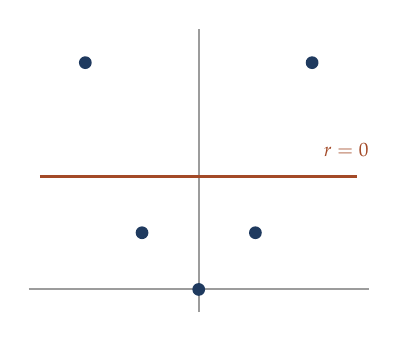
\begin{tikzpicture}[scale=0.72]
\draw[grau!60, line width=0.7pt] (-3,0) -- (3,0);
\draw[grau!60, line width=0.7pt] (0,-0.4) -- (0,4.6);
\foreach \x/\y in {-2/4, -1/1, 0/0, 1/1, 2/4} \fill[tief] (\x,\y) circle (3.2pt);
\draw[akzent, line width=1.1pt] (-2.8,2) -- (2.8,2);
\node[font=\scriptsize, color=akzent] at (2.6,2.45) {$r = 0$};
\end{tikzpicture}
\end{center}

\begin{center}
\begin{minipage}{0.88\textwidth}
\kursiv{Die waagerechte Gerade ist die Regressionsgerade dieser Daten. Sie ist rechnerisch korrekt und inhaltlich Unsinn --- genau das meint Anscombe.}
\end{minipage}
\end{center}
\end{warnung}

\section{Die Rangkorrelation nach Spearman}

\begin{definition}
\boxtitelm{Definition 3.5}
Die \Begriff{Spearman-Korrelation} $r_s$ ist die Pearson-Korrelation der \kursiv{Rangzahlen} statt der Werte. Bei Bindungen vergibt man Durchschnittsränge.

Ohne Bindungen vereinfacht sich die Formel zu
\[ r_s = 1 - \frac{6\sum_i d_i^2}{n(n^2-1)} , \]
wobei $d_i$ die Rangdifferenz der $i$-ten Beobachtung ist.
\end{definition}

\begin{merksatz}
\boxtitel{Warum man das tut}
\begin{center}
\renewcommand{\arraystretch}{1.5}
\begin{tabular}{@{}P{2.8cm}P{5.8cm}@{}}
\toprule
\textbf{Ordinale Daten} & Ränge sind bei ordinalen Merkmalen zulässig, Werte nicht.\\
\textbf{Robustheit} & Ein Ausreißer bekommt den Rang $n$, nicht den Wert $1000$. Der Bruchpunkt steigt erheblich.\\
\textbf{Monotonie statt Linearität} & $r_s$ erfasst jeden \kursiv{gleichsinnigen} Zusammenhang, auch gekrümmte.\\
\bottomrule
\end{tabular}
\end{center}

\schritt{Das Beispiel $y = x^3$}
Für $x = 1,2,3,4,5$ und $y = 1,8,27,64,125$ ist $r \approx 0{,}98$ --- nicht $1$, weil der Zusammenhang nicht linear ist.

Die Ränge sind aber beidemal $1,2,3,4,5$, also $r_s = 1$ exakt. Die Rangkorrelation erkennt den Zusammenhang als das, was er ist: streng monoton.
\end{merksatz}

\begin{merksatz}
\boxtitel{$r_s$ für die MOBIL-Daten}
\schritt{Schritt 1 --- Ränge vergeben}
Die NRS-Werte sortiert: $2,2,3,3,3,4,4,5,5,5,6,7$. Bindungen bekommen Durchschnittsränge:
\begin{center}
{\small
\renewcommand{\arraystretch}{1.35}
\begin{tabular}{@{}P{1.4cm}P{2.6cm}P{2.4cm}@{}}
\toprule
\textbf{NRS} & \textbf{Plätze} & \textbf{Rang}\\
\midrule
$2$ & $1, 2$ & $1{,}5$\\
$3$ & $3, 4, 5$ & $4$\\
$4$ & $6, 7$ & $6{,}5$\\
$5$ & $8, 9, 10$ & $9$\\
$6$ & $11$ & $11$\\
$7$ & $12$ & $12$\\
\bottomrule
\end{tabular}}
\end{center}
Die MOB-Werte sind alle verschieden und bekommen die Ränge $1$ bis $12$.

\schritt{Schritt 2 --- Die Rangtabelle}
\begin{center}
{\small
\renewcommand{\arraystretch}{1.28}
\begin{tabular}{@{}P{0.9cm}P{1.4cm}P{1.4cm}P{1.2cm}P{1.3cm}@{}}
\toprule
\textbf{ID} & $R(x)$ & $R(y)$ & $d$ & $d^2$\\
\midrule
$1$ & $9$ & $10$ & $-1$ & $1$\\
$2$ & $4$ & $5$ & $-1$ & $1$\\
$3$ & $11$ & $11$ & $0$ & $0$\\
$4$ & $6{,}5$ & $9$ & $-2{,}5$ & $6{,}25$\\
$5$ & $12$ & $12$ & $0$ & $0$\\
$6$ & $9$ & $7$ & $2$ & $4$\\
$7$ & $4$ & $4$ & $0$ & $0$\\
$8$ & $1{,}5$ & $2$ & $-0{,}5$ & $0{,}25$\\
$9$ & $6{,}5$ & $6$ & $0{,}5$ & $0{,}25$\\
$10$ & $4$ & $3$ & $1$ & $1$\\
$11$ & $9$ & $8$ & $1$ & $1$\\
$12$ & $1{,}5$ & $1$ & $0{,}5$ & $0{,}25$\\
\midrule
$\sum$ & & & $\mathbf{0}$ & $\mathbf{15{,}0}$\\
\bottomrule
\end{tabular}}
\end{center}

Die Rangdifferenzen summieren sich zu null --- das muss so sein, weil beide Rangsummen gleich sind. Eine gute Rechenprobe.

\schritt{Schritt 3 --- Einsetzen}
\[ r_s \approx 1 - \frac{6 \cdot 15}{12(144-1)} = 1 - \frac{90}{12 \cdot 143} = 1 - \frac{90}{1716} = 1 - 0{,}0524 = \mathbf{0{,}948} . \]

\schritt{Schritt 4 --- Ein Vorbehalt}
Die Kurzformel setzt voraus, dass keine Bindungen vorliegen. Hier gibt es welche, der Wert ist also eine Näherung. Exakt wäre die Pearson-Korrelation der Ränge; sie ergibt $0{,}950$.

\begin{center}
\begin{minipage}{0.88\textwidth}
\kursiv{Der Unterschied ist hier belanglos. Bei vielen Bindungen --- etwa bei einer fünfstufigen Skala und $n = 200$ --- wird er erheblich, und die Kurzformel ist dann falsch. Statistikprogramme rechnen daher stets die lange Fassung.}
\end{minipage}
\end{center}

\schritt{Der Vergleich}
\begin{center}
\renewcommand{\arraystretch}{1.45}
\begin{tabular}{@{}P{3.0cm}P{2.0cm}P{2.8cm}@{}}
\toprule
Pearson $r$ & $0{,}961$ & setzt Linearität voraus\\
Spearman $r_s$ & $0{,}950$ & setzt nur Monotonie voraus\\
\bottomrule
\end{tabular}
\end{center}

Beide sind hoch und fast gleich --- ein Hinweis darauf, dass der Zusammenhang tatsächlich annähernd linear ist. Weichen sie stark voneinander ab, liegt Krümmung oder ein Ausreißer vor.
\end{merksatz}

\section{Korrelation und Ursache}

Nun die wichtigste Seite dieses Bandes.

\begin{warnung}
\boxtitelr{Vier Erklärungen für jede beobachtete Korrelation}
Findet man zwischen $X$ und $Y$ einen Zusammenhang, so kommen stets \kursiv{mindestens} vier Erklärungen infrage.

\begin{center}
\renewcommand{\arraystretch}{1.55}
\begin{tabular}{@{}P{1.0cm}P{2.4cm}P{5.0cm}@{}}
\toprule
$1$ & \textbf{Zufall} & Bei genügend vielen geprüften Merkmalspaaren findet man immer etwas.\\
$2$ & \textbf{$X$ wirkt auf $Y$} & Die erhoffte Erklärung.\\
$3$ & \textbf{$Y$ wirkt auf $X$} & Die Richtung ist aus der Korrelation nicht ablesbar.\\
$4$ & \textbf{Eine dritte Größe} & Ein \Begriff{Konfounder} $Z$ wirkt auf beide.\\
\bottomrule
\end{tabular}
\end{center}

\begin{center}
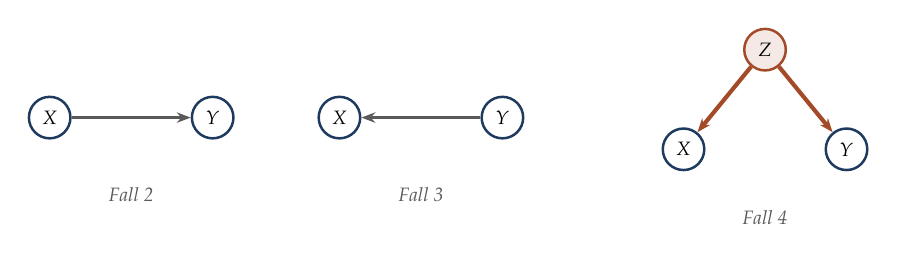
\begin{tikzpicture}[scale=1.15]
\begin{scope}
\node[knotenb] (x) at (-0.9,0) {$X$};
\node[knotenb] (y) at (0.9,0) {$Y$};
\draw[kante, -{Stealth[length=5pt]}] (x) -- (y);
\node[font=\scriptsize\itshape, color=grau] at (0,-0.85) {Fall 2};
\end{scope}
\begin{scope}[xshift=3.2cm]
\node[knotenb] (x2) at (-0.9,0) {$X$};
\node[knotenb] (y2) at (0.9,0) {$Y$};
\draw[kante, -{Stealth[length=5pt]}] (y2) -- (x2);
\node[font=\scriptsize\itshape, color=grau] at (0,-0.85) {Fall 3};
\end{scope}
\begin{scope}[xshift=7.0cm]
\node[knotenb] (x3) at (-0.9,-0.35) {$X$};
\node[knotenb] (y3) at (0.9,-0.35) {$Y$};
\node[knotenr] (z3) at (0,0.75) {$Z$};
\draw[kanted, -{Stealth[length=5pt]}] (z3) -- (x3);
\draw[kanted, -{Stealth[length=5pt]}] (z3) -- (y3);
\node[font=\scriptsize\itshape, color=grau] at (0,-1.1) {Fall 4};
\end{scope}
\end{tikzpicture}
\end{center}

\begin{center}
\begin{minipage}{0.88\textwidth}
\kursiv{Die Korrelation ist in allen vier Fällen \kursiv{dieselbe Zahl}. Sie kann die Fälle nicht unterscheiden --- das ist keine Schwäche der Rechnung, sondern eine Eigenschaft der Daten. Nur das Studiendesign kann hier weiterhelfen; Kapitel~12 zeigt, wie.}
\end{minipage}
\end{center}
\end{warnung}

\begin{merksatz}
\boxtitel{Am MOBIL-Beispiel durchgespielt}
Wir fanden $r = 0{,}96$ zwischen Schmerz und Mobilisationszeit. Welche der vier Erklärungen?

\begin{center}
{\small
\renewcommand{\arraystretch}{1.5}
\begin{tabular}{@{}P{2.2cm}P{6.2cm}@{}}
\toprule
\textbf{Zufall} & Bei $n=12$ und $r = 0{,}96$ unwahrscheinlich, aber nicht ausgeschlossen. Teil~III beziffert das.\\
\textbf{Schmerz $\to$ Zeit} & Plausibel: Wer Schmerzen hat, steht nicht auf.\\
\textbf{Zeit $\to$ Schmerz} & \kursiv{Ebenfalls plausibel:} Wer länger liegt, versteift und hat mehr Schmerz. Die Richtung ist nicht entscheidbar.\\
\textbf{Dritte Größe} & Ein schwieriger Eingriff verursacht beides --- mehr Schmerz \kursiv{und} spätere Mobilisation.\\
\bottomrule
\end{tabular}}
\end{center}

\begin{center}
\begin{minipage}{0.88\textwidth}
\kursiv{Die dritte Zeile ist die lehrreichste. Beide Richtungen sind medizinisch sinnvoll, und die Daten enthalten keine Auskunft darüber, welche zutrifft. Wer aus dieser Korrelation eine Empfehlung ableitet --- \enquote{bessere Analgesie mobilisiert früher} ---, hat eine Annahme hinzugefügt, die nicht in den Daten steht.}
\end{minipage}
\end{center}
\end{merksatz}

\section{Das Simpson-Paradoxon}

Der schärfste Fall von Fall 4 --- und der einzige, bei dem sich ein Zusammenhang durch Aufteilen sogar \kursiv{umkehrt}.

\begin{merksatz}
\boxtitel{Der klassische Datensatz}
Charig und Mitarbeiter verglichen 1986 zwei Verfahren zur Behandlung von Nierensteinen. Die Erfolgsraten:

\begin{center}
{\small
\renewcommand{\arraystretch}{1.48}
\begin{tabular}{@{}P{2.6cm}P{2.6cm}P{2.6cm}@{}}
\toprule
& \textbf{Verfahren A} & \textbf{Verfahren B}\\
\midrule
Kleine Steine & $81/87 = 93\,\%$ & $234/270 = 87\,\%$\\
Große Steine & $192/263 = 73\,\%$ & $55/80 = 69\,\%$\\
\midrule
\textbf{Gesamt} & $273/350 = \mathbf{78\,\%}$ & $289/350 = \mathbf{83\,\%}$\\
\bottomrule
\end{tabular}}
\end{center}

\begin{center}
\begin{minipage}{0.9\textwidth}
\textbf{A ist in beiden Gruppen besser --- und insgesamt schlechter.}
\end{minipage}
\end{center}
\end{merksatz}

\begin{merksatz}
\boxtitel{Warum das geht --- die Rechnung}
\schritt{Schritt 1 --- Nachprüfen, dass die Zahlen stimmen}
Verfahren A gesamt: $81 + 192 = 273$ Erfolge bei $87 + 263 = 350$ Fällen. $273/350 = 0{,}78$. \checkmark\\
Verfahren B gesamt: $234 + 55 = 289$ bei $270 + 80 = 350$. $289/350 = 0{,}826$. \checkmark

\schritt{Schritt 2 --- Die Ursache finden}
Entscheidend ist die \kursiv{Verteilung der Fälle} auf die Schweregrade:

\begin{center}
\renewcommand{\arraystretch}{1.45}
\begin{tabular}{@{}P{2.4cm}P{2.2cm}P{2.2cm}@{}}
\toprule
& \textbf{A} & \textbf{B}\\
\midrule
Kleine Steine & $87$ ($25\,\%$) & $270$ ($77\,\%$)\\
Große Steine & $263$ ($75\,\%$) & $80$ ($23\,\%$)\\
\bottomrule
\end{tabular}
\end{center}

Verfahren A wurde überwiegend bei den \kursiv{schwierigen} Fällen angewandt, B überwiegend bei den leichten.

\schritt{Schritt 3 --- Der Gesamtwert als gewichtetes Mittel}
Die Gesamtrate ist das mit den Fallzahlen gewichtete Mittel der beiden Teilraten:
\[ A: \quad \frac{87}{350}\cdot 0{,}93 + \frac{263}{350}\cdot 0{,}73 = 0{,}249 \cdot 0{,}93 + 0{,}751 \cdot 0{,}73 = 0{,}231 + 0{,}549 = 0{,}780 \]
\[ B: \quad \frac{270}{350}\cdot 0{,}87 + \frac{80}{350}\cdot 0{,}69 = 0{,}771 \cdot 0{,}87 + 0{,}229 \cdot 0{,}69 = 0{,}671 + 0{,}158 = 0{,}829 \]

\schritt{Schritt 4 --- Die Erklärung in einem Satz}
\begin{center}
\begin{minipage}{0.9\textwidth}
A ist überall besser, wird aber überwiegend auf die schwere Gruppe angewandt, in der \kursiv{beide} Verfahren schlechter abschneiden. Die Gewichtung schlägt den Vorteil.
\end{minipage}
\end{center}

\begin{center}
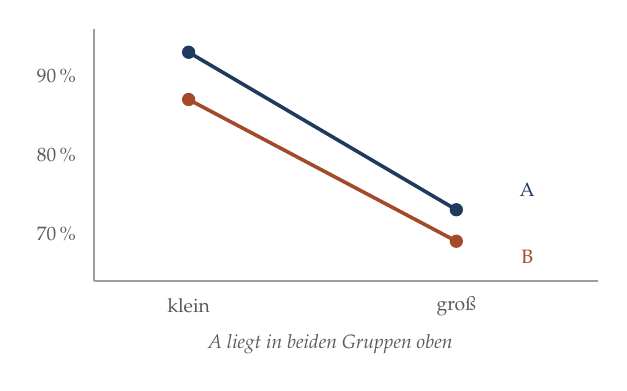
\begin{tikzpicture}[scale=1.0]
\draw[grau!60, line width=0.7pt] (0,0) -- (6.4,0);
\draw[grau!60, line width=0.7pt] (0,0) -- (0,3.2);
\node[font=\scriptsize, color=grau] at (1.2,-0.32) {klein};
\node[font=\scriptsize, color=grau] at (4.6,-0.32) {groß};
\foreach \y/\lab in {0.6/70, 1.6/80, 2.6/90}
  \node[font=\scriptsize, color=grau] at (-0.48,\y) {\lab\,\%};
\draw[tief, line width=1.3pt] (1.2,2.9) -- (4.6,0.9);
\draw[akzent, line width=1.3pt] (1.2,2.3) -- (4.6,0.5);
\fill[tief] (1.2,2.9) circle (2.4pt); \fill[tief] (4.6,0.9) circle (2.4pt);
\fill[akzent] (1.2,2.3) circle (2.4pt); \fill[akzent] (4.6,0.5) circle (2.4pt);
\node[font=\scriptsize, color=tief] at (5.5,1.15) {A};
\node[font=\scriptsize, color=akzent] at (5.5,0.3) {B};
\node[font=\scriptsize\itshape, color=grau] at (3.0,-0.8) {A liegt in beiden Gruppen oben};
\end{tikzpicture}
\end{center}
\end{merksatz}

\begin{warnung}
\boxtitelr{Welche Zahl gilt nun?}
Diese Frage lässt sich \kursiv{nicht} statistisch beantworten. Sie hängt davon ab, was man wissen will.

\begin{center}
\renewcommand{\arraystretch}{1.55}
\begin{tabular}{@{}P{2.8cm}P{5.8cm}@{}}
\toprule
\textbf{\enquote{Welches Verfahren soll ich wählen?}} & Die \kursiv{getrennten} Raten. Der Steindurchmesser ist vor der Behandlung bekannt; man entscheidet innerhalb seiner Gruppe. \textbf{Antwort: A.}\\
\textbf{\enquote{Wie erfolgreich war Klinik X?}} & Die Gesamtrate --- aber sie sagt mehr über die Fallauswahl als über das Verfahren.\\
\bottomrule
\end{tabular}
\end{center}

\begin{center}
\begin{minipage}{0.88\textwidth}
\kursiv{Die Regel lautet: Man teilt nach einer Größe auf, die \kursiv{vor} der Behandlung feststand und beide beeinflusst --- hier die Steingröße. Teilt man dagegen nach einer Größe auf, die \kursiv{durch} die Behandlung entstanden ist, macht man es schlimmer. Welcher Fall vorliegt, entscheidet das Fachwissen, nicht die Rechnung.}
\end{minipage}
\end{center}
\end{warnung}

\begin{warnung}
\boxtitelr{Der ökologische Fehlschluss}
Eine verwandte Falle: Zusammenhänge auf Gruppenebene gelten nicht notwendig für Einzelne.

\schritt{Das klassische Beispiel}
Vergleicht man Bundesländer, so ist der Anteil der Menschen mit hohem Bildungsabschluss oft positiv mit einer bestimmten Wahlpräferenz korreliert. Daraus folgt \kursiv{nicht}, dass gebildete Personen so wählen --- der Zusammenhang kann auf Ebene der Personen sogar umgekehrt sein.

\begin{center}
\begin{minipage}{0.88\textwidth}
\kursiv{In der Medizin tritt derselbe Fehler auf, wenn man aus Länderdaten --- \enquote{Länder mit hohem Fischkonsum haben niedrigere Herzinfarktraten} --- auf den einzelnen Menschen schließt. Solche Studien heißen \Begriff{ökologische Studien}; sie erzeugen Hypothesen und belegen nichts. Kapitel~12 ordnet sie in die Hierarchie der Studientypen ein.}
\end{minipage}
\end{center}
\end{warnung}

\section{Übungsaufgaben}

\begin{aufgabe}
\boxtitel{Aufgabe 3.1 --- Korrelation von Hand}
Bestimmen Sie $r$ zwischen \code{ALTER} und \code{MOB} für die sechs Beobachtungen der Gruppe A und deuten Sie das Ergebnis.

\loesung
\schritt{Schritt 1 --- Die Tabelle}
\begin{center}
{\small
\renewcommand{\arraystretch}{1.3}
\begin{tabular}{@{}P{1.2cm}P{1.2cm}P{1.4cm}P{1.4cm}P{1.4cm}@{}}
\toprule
$x$ (Alter) & $y$ (MOB) & $x^2$ & $y^2$ & $xy$\\
\midrule
$68$ & $26$ & $4624$ & $676$ & $1768$\\
$74$ & $19$ & $5476$ & $361$ & $1406$\\
$61$ & $31$ & $3721$ & $961$ & $1891$\\
$79$ & $24$ & $6241$ & $576$ & $1896$\\
$70$ & $35$ & $4900$ & $1225$ & $2450$\\
$65$ & $22$ & $4225$ & $484$ & $1430$\\
\midrule
$\mathbf{417}$ & $\mathbf{157}$ & $\mathbf{29187}$ & $\mathbf{4283}$ & $\mathbf{10841}$\\
\bottomrule
\end{tabular}}
\end{center}

\schritt{Schritt 2 --- Die drei Summen}
\[ \sum(x-\MW)^2 = 29187 - \frac{417^2}{6} = 29187 - \frac{173889}{6} = 29187 - 28981{,}5 = 205{,}5 \]
\[ \sum(y-\overline y)^2 = 4283 - \frac{157^2}{6} = 4283 - 4108{,}17 = 174{,}83 \]
\[ \sum(x-\MW)(y-\overline y) = 10841 - \frac{417 \cdot 157}{6} = 10841 - \frac{65469}{6} = 10841 - 10911{,}5 = -70{,}5 \]

\schritt{Schritt 3 --- Einsetzen}
\[ r = \frac{-70{,}5}{\sqrt{205{,}5}\cdot\sqrt{174{,}83}} = \frac{-70{,}5}{14{,}336 \cdot 13{,}222} = \frac{-70{,}5}{189{,}55} \approx \mathbf{-0{,}372} . \]

\schritt{Schritt 4 --- Die Deutung, sorgfältig}
\begin{center}
\renewcommand{\arraystretch}{1.5}
\begin{tabular}{@{}P{2.4cm}P{6.2cm}@{}}
\toprule
\textbf{Vorzeichen} & negativ --- Ältere mobilisieren in diesen sechs Fällen \kursiv{früher}.\\
\textbf{Betrag} & $0{,}37$ --- schwach bis mäßig.\\
\textbf{Stichprobe} & $n = 6$. Das ist der entscheidende Punkt.\\
\bottomrule
\end{tabular}
\end{center}

\schritt{Schritt 5 --- Warum man hier nichts schließen darf}
Bei $n = 6$ ergeben sich aus reinem Zufall regelmäßig Korrelationen dieser Größenordnung. Teil~III wird zeigen: Für einen Nachweis bräuchte man bei $n=6$ einen Betrag über etwa $0{,}81$.

\begin{center}
\begin{minipage}{0.86\textwidth}
\kursiv{Das Ergebnis widerspricht auch der Erwartung --- man würde vermuten, dass Ältere \kursiv{später} mobilisieren. Genau bei solchen Befunden ist die Versuchung am größten, eine Erklärung zu erfinden. Die richtige Reaktion ist: zu wenige Daten, keine Aussage.}
\end{minipage}
\end{center}
\end{aufgabe}

\begin{aufgabe}
\boxtitel{Aufgabe 3.2 --- Ein eigenes Simpson-Beispiel bauen}
Konstruieren Sie zwei Krankenhäuser, bei denen Haus A in beiden Schweregraden eine niedrigere Sterblichkeit hat als Haus B, insgesamt aber eine höhere.

\loesung
\schritt{Schritt 1 --- Die Bauanleitung}
Man braucht:
\begin{center}
\renewcommand{\arraystretch}{1.5}
\begin{tabular}{@{}P{1.0cm}P{7.4cm}@{}}
\toprule
(a) & Zwei Schweregrade mit deutlich verschiedener Sterblichkeit.\\
(b) & Haus A behandelt überwiegend schwere Fälle, Haus B überwiegend leichte.\\
(c) & In jedem Schweregrad ist A ein wenig besser.\\
\bottomrule
\end{tabular}
\end{center}

\schritt{Schritt 2 --- Zahlen wählen}
Leichte Fälle: Sterblichkeit um $2\,\%$. Schwere: um $30\,\%$.

\begin{center}
{\small
\renewcommand{\arraystretch}{1.45}
\begin{tabular}{@{}P{2.2cm}P{2.8cm}P{2.8cm}@{}}
\toprule
& \textbf{Haus A} & \textbf{Haus B}\\
\midrule
Leicht & $2/100 = 2{,}0\,\%$ & $27/900 = 3{,}0\,\%$\\
Schwer & $270/900 = 30{,}0\,\%$ & $31/100 = 31{,}0\,\%$\\
\midrule
\textbf{Gesamt} & $272/1000 = \mathbf{27{,}2\,\%}$ & $58/1000 = \mathbf{5{,}8\,\%}$\\
\bottomrule
\end{tabular}}
\end{center}

\schritt{Schritt 3 --- Prüfen}
Leicht: $2{,}0 < 3{,}0$ --- A besser. \checkmark\\
Schwer: $30{,}0 < 31{,}0$ --- A besser. \checkmark\\
Gesamt: $27{,}2 > 5{,}8$ --- A \kursiv{deutlich} schlechter. \checkmark

\schritt{Schritt 4 --- Die Deutung}
Haus A ist ein Maximalversorger: Neunzig Prozent seiner Fälle sind schwer. Haus B ist eine Belegklinik mit überwiegend leichten Eingriffen.

Die Gesamtsterblichkeit misst hier fast ausschließlich die \kursiv{Fallzusammensetzung} und fast nichts von der Behandlungsqualität.

\begin{center}
\begin{minipage}{0.86\textwidth}
\kursiv{Genau darum werden Qualitätskennzahlen im Gesundheitswesen \Begriff{risikoadjustiert} angegeben --- man rechnet auf eine gemeinsame Fallzusammensetzung um. Ohne diese Bereinigung bestraft jede Rangliste die Häuser, die die schweren Fälle übernehmen.}
\end{minipage}
\end{center}

\schritt{Schritt 5 --- Die Umrechnung vorführen}
Wir standardisieren auf eine gedachte Bevölkerung mit je $500$ leichten und $500$ schweren Fällen:
\[ A: \quad 0{,}5 \cdot 2{,}0\,\% + 0{,}5 \cdot 30{,}0\,\% = 16{,}0\,\% \]
\[ B: \quad 0{,}5 \cdot 3{,}0\,\% + 0{,}5 \cdot 31{,}0\,\% = 17{,}0\,\% \]
Bei gleicher Fallzusammensetzung ist A besser --- wie es die Teilraten sagen. \checkmark
\end{aufgabe}

\begin{aufgabe}
\boxtitel{Aufgabe 3.3 --- Pearson gegen Spearman}
Gegeben seien die Wertepaare
\[ (1,1),\ (2,2),\ (3,3),\ (4,4),\ (5,50) . \]
Berechnen Sie $r$ und $r_s$ und erklären Sie den Unterschied.

\loesung
\schritt{Schritt 1 --- Pearson}
\begin{center}
{\small
\renewcommand{\arraystretch}{1.3}
\begin{tabular}{@{}P{1.0cm}P{1.2cm}P{1.2cm}P{1.4cm}P{1.4cm}@{}}
\toprule
$x$ & $y$ & $x^2$ & $y^2$ & $xy$\\
\midrule
$1$ & $1$ & $1$ & $1$ & $1$\\
$2$ & $2$ & $4$ & $4$ & $4$\\
$3$ & $3$ & $9$ & $9$ & $9$\\
$4$ & $4$ & $16$ & $16$ & $16$\\
$5$ & $50$ & $25$ & $2500$ & $250$\\
\midrule
$\mathbf{15}$ & $\mathbf{60}$ & $\mathbf{55}$ & $\mathbf{2530}$ & $\mathbf{280}$\\
\bottomrule
\end{tabular}}
\end{center}

\[ \sum(x-\MW)^2 = 55 - \frac{225}{5} = 55 - 45 = 10 \]
\[ \sum(y-\overline y)^2 = 2530 - \frac{3600}{5} = 2530 - 720 = 1810 \]
\[ \sum(x-\MW)(y-\overline y) = 280 - \frac{15 \cdot 60}{5} = 280 - 180 = 100 \]
\[ r = \frac{100}{\sqrt{10}\cdot\sqrt{1810}} = \frac{100}{3{,}162 \cdot 42{,}544} = \frac{100}{134{,}54} \approx \mathbf{0{,}743} \]

\schritt{Schritt 2 --- Spearman}
Die Ränge sind in beiden Merkmalen $1,2,3,4,5$ --- keine Bindungen, alle Differenzen null:
\[ r_s = 1 - \frac{6 \cdot 0}{5 \cdot 24} = \mathbf{1{,}000} . \]

\schritt{Schritt 3 --- Der Vergleich}
\begin{center}
\renewcommand{\arraystretch}{1.48}
\begin{tabular}{@{}P{2.4cm}P{1.8cm}P{4.0cm}@{}}
\toprule
Pearson & $0{,}743$ & misst Nähe zur \kursiv{Geraden}\\
Spearman & $\mathbf{1{,}000}$ & misst \kursiv{Monotonie}\\
\bottomrule
\end{tabular}
\end{center}

\schritt{Schritt 4 --- Die Erklärung}
Der Zusammenhang ist \kursiv{perfekt monoton}: Jedes größere $x$ geht mit einem größeren $y$ einher, ohne Ausnahme. Spearman erkennt das exakt.

Pearson misst etwas anderes --- die Nähe zu einer Geraden. Der Sprung von $4$ auf $50$ passt zu keiner Geraden, die auch die ersten vier Punkte trifft. Deshalb bleibt $r$ deutlich unter $1$.

\schritt{Schritt 5 --- Was daraus zu lernen ist}
\begin{center}
\begin{minipage}{0.9\textwidth}
\textbf{Ein niedrigeres $r$ bedeutet nicht \enquote{schwächerer Zusammenhang}, sondern \enquote{weniger geradlinig}.} Wer $r$ als Maß für die Stärke des Zusammenhangs liest, verwechselt beides.
\end{minipage}
\end{center}

\schritt{Nachbemerkung --- welche Zahl hier die richtige ist}
Das hängt von der Frage ab. Will man wissen, ob $y$ mit $x$ zunimmt: Spearman. Will man $y$ aus $x$ durch eine lineare Formel vorhersagen: Pearson --- und die Antwort $0{,}743$ ist dann die ehrliche Auskunft, dass eine Gerade hier schlecht passt.
\end{aufgabe}

\begin{geschichte}
\boxtitelg{Galton, Pearson und ein Erbe mit zwei Seiten}
\Person{Francis Galton} (1822--1911) stieß auf die Korrelation bei der Untersuchung von Körpergrößen in Familien. Er bemerkte, dass die Kinder großer Eltern im Mittel kleiner sind als diese --- und die Kinder kleiner Eltern größer. Er nannte das \kursiv{regression towards mediocrity}; daher stammt das Wort \enquote{Regression}, das heute etwas ganz anderes bezeichnet.

\Person{Karl Pearson} (1857--1936), Galtons Schüler, gab der Korrelation 1896 die heutige Formel und baute daraus die mathematische Statistik als Fach auf. Er gründete 1901 die Zeitschrift \kursiv{Biometrika} und besetzte 1911 den ersten Lehrstuhl für Statistik.

\begin{center}
\begin{minipage}{0.9\textwidth}
\kursiv{Beide waren führende Vertreter der Eugenik --- Galton prägte den Begriff, Pearson vertrat ihn in einer Schärfe, die auch nach den Maßstäben seiner Zeit auffiel. Der Lehrstuhl, den Pearson innehatte, war aus einer eugenischen Stiftung Galtons hervorgegangen; das University College London benannte 2020 die nach beiden benannten Gebäude um.}
\end{minipage}
\end{center}

Die Werkzeuge sind davon unberührt --- eine Formel trägt keine Gesinnung. Die Geschichte gehört trotzdem dazu, und zwar aus einem sachlichen Grund: Der Anlass, aus dem heraus die Korrelation entwickelt wurde, war die Frage nach der Vererbung von Eigenschaften. Genau dort ist die Verwechslung von Zusammenhang und Ursache am folgenreichsten --- und sie wurde damals begangen.
\end{geschichte}

\begin{forschung}
\boxtitelp{Von der Korrelation zur Kausalität}
Die Frage, wann man aus Daten auf Ursachen schließen darf, war jahrzehntelang kein mathematisches Thema --- man hielt sie für unentscheidbar und überließ sie dem Studiendesign.

Das hat sich geändert. \Person{Judea Pearl} entwickelte seit den 1990er Jahren einen Formalismus, der kausale Annahmen in einem gerichteten Graphen aufschreibt --- einem \Begriff{DAG}, wie er in Band 16, Kapitel~12 vorkommt. Aus der Struktur dieses Graphen lässt sich dann \kursiv{ausrechnen}, welche Größen man kontrollieren muss und welche man gerade nicht kontrollieren darf.

\begin{center}
{\small
\renewcommand{\arraystretch}{1.45}
\begin{tabular}{@{}P{2.6cm}P{5.6cm}@{}}
\toprule
\textbf{Konfounder} & wirkt auf Ursache und Wirkung --- \textcolor{gruen}{muss} berücksichtigt werden\\
\textbf{Mediator} & liegt auf dem Wirkungsweg --- \textcolor{akzent}{darf nicht} berücksichtigt werden\\
\textbf{Kollider} & wird von beiden beeinflusst --- \textcolor{akzent}{erzeugt} bei Berücksichtigung einen Scheinzusammenhang\\
\bottomrule
\end{tabular}}
\end{center}

Die dritte Zeile war die Überraschung: Das Berücksichtigen einer weiteren Größe kann einen Zusammenhang \kursiv{erzeugen}, der ohne sie nicht besteht. Das widerspricht der verbreiteten Vorstellung, mehr Kontrollvariablen seien immer besser.

Pearl erhielt 2011 den Turing-Preis. Kapitel~15 kommt darauf zurück.

\begin{center}
\begin{minipage}{0.88\textwidth}
\kursiv{Für die Praxis heißt das: Ob eine Größe in ein Modell gehört, ist keine statistische Frage. Sie entscheidet sich an der vermuteten Wirkungsstruktur --- und die muss man aufschreiben, bevor man rechnet.}
\end{minipage}
\end{center}
\end{forschung}

\begin{merksatz}
\boxtitel{Was Sie jetzt können}
\begin{center}
\renewcommand{\arraystretch}{1.5}
\begin{tabular}{@{}P{3.0cm}P{5.6cm}@{}}
\toprule
\textbf{Definition 3.1} & Kovarianz --- und warum sie allein unbrauchbar ist\\
\textbf{Satz 3.4} & $-1 \le r \le 1$, mit Gleichheit genau bei exakter Geradenlage\\
\textbf{Definition 3.5} & Spearman: Monotonie statt Linearität\\
\textbf{Vier Erklärungen} & Zufall, Wirkung, Gegenwirkung, dritte Größe\\
\textbf{Simpson} & Ein Zusammenhang kann sich beim Aufteilen umkehren\\
\bottomrule
\end{tabular}
\end{center}

\begin{center}
\begin{minipage}{0.88\textwidth}
\kursiv{Damit endet Teil~I. Bisher haben wir nur beschrieben, was in den Daten steht. Ab Kapitel~4 fragen wir, was sie über die Grundgesamtheit sagen --- und dort beginnt die eigentliche Statistik.}
\end{minipage}
\end{center}
\end{merksatz}

\part{Schätzen}

\chapter{Von der Stichprobe zur Aussage}

\section{Der Sprung}

Bis hierhin haben wir beschrieben, was in zwölf Zeilen einer Tabelle steht. Das ist unstrittig: Der Mittelwert der Gruppe B beträgt $18{,}0$ Stunden, und daran gibt es nichts zu deuten.

Die Frage, die eine Studie stellt, ist eine andere.

\begin{merksatz}
\boxtitel{Zwei Fragen, die man auseinanderhalten muss}
\begin{center}
\renewcommand{\arraystretch}{1.55}
\begin{tabular}{@{}P{2.6cm}P{6.0cm}@{}}
\toprule
\textbf{Beschreibend} & Wie lange brauchten \kursiv{diese sechs} Personen? --- $18{,}0$ Stunden im Mittel. Fertig.\\
\textbf{Schließend} & Wie lange braucht ein Mensch nach diesem Schema \kursiv{im Allgemeinen}? --- Darauf gibt es keine sichere Antwort.\\
\bottomrule
\end{tabular}
\end{center}

\begin{center}
\begin{minipage}{0.88\textwidth}
\kursiv{Der Sprung von der ersten zur zweiten Frage ist der Gegenstand der gesamten restlichen Teile dieses Bandes. Er ist nie sicher, und die Kunst besteht darin, die verbleibende Unsicherheit zu \kursiv{beziffern} statt sie zu verschweigen.}
\end{minipage}
\end{center}
\end{merksatz}

\begin{definition}
\boxtitelm{Definition 4.1 --- Grundgesamtheit und Stichprobe}
\begin{itemize}[leftmargin=1.4em, itemsep=4pt]
\item Die \Begriff{Grundgesamtheit} ist die Menge aller Objekte, über die eine Aussage gemacht werden soll.
\item Eine \Begriff{Stichprobe} ist eine Teilmenge davon, die tatsächlich untersucht wird.
\item Eine Kennzahl der Grundgesamtheit heißt \Begriff{Parameter}; eine aus der Stichprobe berechnete heißt \Begriff{Schätzer} oder \Begriff{Statistik}.
\end{itemize}
\end{definition}

\begin{merksatz}
\boxtitel{Die Bezeichnungen --- und warum sie streng getrennt werden}
\begin{center}
{\small
\renewcommand{\arraystretch}{1.5}
\begin{tabular}{@{}P{3.2cm}P{1.8cm}P{1.8cm}P{1.4cm}@{}}
\toprule
& \textbf{Parameter} & \textbf{Schätzer} & \\
\midrule
Mittelwert & $\mu$ & $\MW$ & \\
Standard\-abweichung & $\sigma$ & $s$ & \\
Anteil & $\pi$ & $\hat{p}$ & \\
Korrelation & $\rho$ & $r$ & \\
Umfang & $N$ & $n$ & \\
\bottomrule
\end{tabular}}
\end{center}

\begin{center}
\renewcommand{\arraystretch}{1.5}
\begin{tabular}{@{}P{2.6cm}P{6.0cm}@{}}
\toprule
\textbf{Parameter} & fest, aber \kursiv{unbekannt}. Er hat einen Wert; wir kennen ihn nicht.\\
\textbf{Schätzer} & bekannt, aber \kursiv{zufällig}. Eine andere Stichprobe hätte einen anderen Wert ergeben.\\
\bottomrule
\end{tabular}
\end{center}

\begin{center}
\begin{minipage}{0.88\textwidth}
\kursiv{Diese Umkehrung ist der Angelpunkt. In der beschreibenden Statistik war $\MW$ eine feste Zahl. Jetzt ist $\MW$ eine \kursiv{Zufallsgröße} und $\mu$ die feste Zahl. Wer das durcheinanderbringt, kommt bei Konfidenzintervallen und $p$-Werten zwangsläufig auf die falschen Deutungen --- beide Fehldeutungen aus dem Vorwort lassen sich genau hierauf zurückführen.}
\end{minipage}
\end{center}
\end{merksatz}

\begin{warnung}
\boxtitelr{Die Grundgesamtheit muss man benennen}
Welche Grundgesamtheit meint die MOBIL-Studie?

\begin{center}
\renewcommand{\arraystretch}{1.5}
\begin{tabular}{@{}P{3.2cm}P{5.4cm}@{}}
\toprule
Alle je operierten Personen dieser Klinik? & Dann ist die Stichprobe nicht zufällig --- sie stammt aus einem Zeitraum.\\
Alle künftigen Personen dieser Klinik? & Dann setzt man voraus, dass sich nichts ändert.\\
Alle Personen mit Hüftgelenksersatz? & Dann müsste die Klinik für alle Kliniken stehen.\\
\bottomrule
\end{tabular}
\end{center}

\begin{center}
\begin{minipage}{0.88\textwidth}
\kursiv{Keine dieser Grundgesamtheiten ist die, aus der tatsächlich zufällig gezogen wurde --- denn es wurde überhaupt nicht zufällig gezogen. Randomisiert wurde nur die \kursiv{Zuteilung} auf die beiden Gruppen, nicht die Auswahl der Personen. Kapitel~12 zeigt, warum das trotzdem ausreicht, und wofür genau.}
\end{minipage}
\end{center}
\end{warnung}

\section{Was wir aus Band 4 brauchen}

Der folgende Abschnitt wiederholt vier Begriffe. Wer Band 4 durchgearbeitet hat, kann ihn überspringen.

\begin{definition}
\boxtitelm{Definition 4.2 --- Zufallsgröße, Erwartungswert, Varianz}
Eine \Begriff{Zufallsgröße} $X$ ist eine Größe, deren Wert vom Zufall abhängt.

Für eine Zufallsgröße mit den möglichen Werten $a_1, a_2, \ldots$ und den Wahrscheinlichkeiten $p_1, p_2, \ldots$ ist
\[ \mathbb{E}[X] = \sum_k a_k\,p_k , \qquad \Var[X] = \mathbb{E}\bigl[(X - \mathbb{E}[X])^2\bigr] . \]
\end{definition}

\begin{merksatz}
\boxtitel{Die Rechenregeln, die wir brauchen}
\begin{center}
\renewcommand{\arraystretch}{1.6}
\begin{tabular}{@{}P{1.0cm}P{4.0cm}P{3.2cm}@{}}
\toprule
(R1) & $\mathbb{E}[aX+b] = a\,\mathbb{E}[X]+b$ & immer\\
(R2) & $\mathbb{E}[X+Y] = \mathbb{E}[X]+\mathbb{E}[Y]$ & \textbf{immer}\\
(R3) & $\Var[aX+b] = a^2\,\Var[X]$ & immer\\
(R4) & $\Var[X+Y] = \Var[X]+\Var[Y]$ & \textcolor{akzent}{\textbf{nur bei Unabhängigkeit}}\\
\bottomrule
\end{tabular}
\end{center}

\schritt{Die entscheidende Asymmetrie}
Regel (R2) gilt ohne jede Voraussetzung --- Erwartungswerte addieren sich stets. Regel (R4) gilt \kursiv{nicht} allgemein; sie verlangt, dass die Zufallsgrößen einander nicht beeinflussen.

\begin{center}
\begin{minipage}{0.88\textwidth}
\kursiv{Ein Gegenbeispiel zu (R4) ohne Unabhängigkeit: Sei $Y = -X$. Dann ist $X+Y = 0$, also $\Var[X+Y] = 0$ --- aber $\Var[X]+\Var[Y] = 2\Var[X] > 0$. Die Regel bricht vollständig zusammen.}
\end{minipage}
\end{center}

\schritt{Warum (R3) das Quadrat hat}
Die Varianz misst quadrierte Abweichungen. Streckt man alle Werte um den Faktor $a$, so verdoppelt sich jede Abweichung um $a$ --- und ihr Quadrat um $a^2$. Die Verschiebung $b$ ändert die Abweichungen nicht und fällt heraus. Das ist genau die Rechnung aus Aufgabe 2.2.
\end{merksatz}

\section{Die Normalverteilung}

\begin{definition}
\boxtitelm{Definition 4.3}
Eine stetige Zufallsgröße $X$ heißt \Begriff{normalverteilt} mit den Parametern $\mu$ und $\sigma > 0$, geschrieben $X \sim \mathcal{N}(\mu, \sigma^2)$, wenn ihre \Begriff{Dichte}
\[ f(x) = \frac{1}{\sigma\sqrt{2\pi}}\;\exp\!\left(-\frac{(x-\mu)^2}{2\sigma^2}\right) \]
lautet. Die Wahrscheinlichkeit, dass $X$ zwischen $a$ und $b$ liegt, ist die \kursiv{Fläche} unter dieser Kurve zwischen $a$ und $b$.
\end{definition}

\begin{merksatz}
\boxtitel{Die Formel, Stück für Stück}
\begin{center}
{\small
\renewcommand{\arraystretch}{1.55}
\begin{tabular}{@{}P{2.6cm}P{6.0cm}@{}}
\toprule
$(x-\mu)^2$ & Der Abstand vom Mittelwert, quadriert. Symmetrisch --- links und rechts gleich.\\
geteilt durch $2\sigma^2$ & Macht den Abstand einheitenfrei und regelt die Breite.\\
$\exp(-\cdot)$ & Macht daraus einen Wert, der bei $x=\mu$ am größten ist und nach außen rasch fällt.\\
$\frac{1}{\sigma\sqrt{2\pi}}$ & Ein Normierungsfaktor, der dafür sorgt, dass die Gesamtfläche genau $1$ beträgt.\\
\bottomrule
\end{tabular}}
\end{center}

\begin{center}
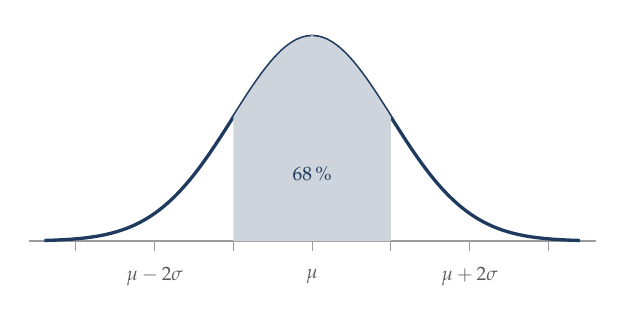
\begin{tikzpicture}[scale=1.0]
\draw[grau!60, line width=0.7pt] (-3.6,0) -- (3.6,0);
\draw[tief, line width=1.2pt, smooth, samples=90, domain=-3.4:3.4]
  plot (\x, {2.6*exp(-\x*\x/2)});
\draw[grau!50, dashed, line width=0.6pt] (0,0) -- (0,2.7);
\foreach \x in {-3,-2,-1,0,1,2,3} \draw[grau!60] (\x,0) -- (\x,-0.12);
\foreach \x/\lab in {-2/{$\mu-2\sigma$}, 0/{$\mu$}, 2/{$\mu+2\sigma$}}
  \node[font=\scriptsize, color=grau] at (\x,-0.45) {\lab};
\fill[tief!22] plot[smooth, samples=40, domain=-1:1] (\x,{2.6*exp(-\x*\x/2)}) -- (1,0) -- (-1,0) -- cycle;
\node[font=\scriptsize, color=tief] at (0,0.85) {$68\,\%$};
\end{tikzpicture}
\end{center}

\schritt{Die drei Merkzahlen}
\begin{center}
\renewcommand{\arraystretch}{1.45}
\begin{tabular}{@{}P{2.8cm}P{2.4cm}P{2.6cm}@{}}
\toprule
\textbf{Bereich} & \textbf{Anteil} & \textbf{genauer}\\
\midrule
$\mu \pm 1\sigma$ & $68\,\%$ & $68{,}27\,\%$\\
$\mu \pm 2\sigma$ & $95\,\%$ & $95{,}45\,\%$\\
$\mu \pm 3\sigma$ & $99{,}7\,\%$ & $99{,}73\,\%$\\
\midrule
$\mu \pm 1{,}96\,\sigma$ & \textbf{genau $95\,\%$} & \\
\bottomrule
\end{tabular}
\end{center}

\begin{center}
\begin{minipage}{0.88\textwidth}
\kursiv{Die letzte Zeile ist die, die man braucht. Die Zahl $1{,}96$ wird Ihnen im ganzen Rest dieses Bandes begegnen --- sie ist der Grund, warum so viele Formeln \enquote{$\pm\,1{,}96$} enthalten.}
\end{minipage}
\end{center}
\end{merksatz}

\begin{merksatz}
\boxtitel{Standardisierung und die Tabelle}
Ist $X \sim \mathcal{N}(\mu,\sigma^2)$, so ist
\[ Z = \frac{X-\mu}{\sigma} \;\sim\; \mathcal{N}(0,1) . \]

\schritt{Warum}
Nach (R1) ist $\mathbb{E}[Z] = \frac{1}{\sigma}(\mu - \mu) = 0$, und nach (R3) ist $\Var[Z] = \frac{1}{\sigma^2}\sigma^2 = 1$. Dass auch die \kursiv{Form} erhalten bleibt, ist eine Eigenschaft der Normalverteilung und wird in Band 4 nachgerechnet.

\schritt{Die Verteilungsfunktion}
Man schreibt $\Phi(z)$ für die Fläche links von $z$ unter der Standardnormalkurve.

\begin{center}
{\small
\renewcommand{\arraystretch}{1.38}
\begin{tabular}{@{}P{1.2cm}P{1.6cm}P{1.2cm}P{1.6cm}@{}}
\toprule
$z$ & $\Phi(z)$ & $z$ & $\Phi(z)$\\
\midrule
$0{,}00$ & $0{,}5000$ & $1{,}64$ & $0{,}9495$\\
$0{,}50$ & $0{,}6915$ & $1{,}96$ & $\mathbf{0{,}9750}$\\
$1{,}00$ & $0{,}8413$ & $2{,}00$ & $0{,}9772$\\
$1{,}28$ & $0{,}8997$ & $2{,}58$ & $0{,}9951$\\
$1{,}50$ & $0{,}9332$ & $3{,}00$ & $0{,}9987$\\
\bottomrule
\end{tabular}}
\end{center}

\schritt{Die Symmetrieregel}
Für negative $z$ braucht man keine eigene Tabelle:
\[ \Phi(-z) = 1 - \Phi(z) . \]
Das folgt daraus, dass die Kurve spiegelsymmetrisch zur Null ist: Die Fläche links von $-z$ ist so groß wie die rechts von $+z$.

\schritt{Eine Rechnung}
Wie groß ist die Wahrscheinlichkeit, dass $Z$ zwischen $-1{,}96$ und $1{,}96$ liegt?
\begin{align*}
\Pr[-1{,}96 \le Z \le 1{,}96] &= \Phi(1{,}96) - \Phi(-1{,}96)\\
&= \Phi(1{,}96) - \bigl(1 - \Phi(1{,}96)\bigr)\\
&= 2\,\Phi(1{,}96) - 1\\
&= 2 \cdot 0{,}9750 - 1 = 0{,}9500 . \quad \checkmark
\end{align*}
\end{merksatz}

\section{Die Stichprobenverteilung des Mittelwerts}

Nun der zentrale Satz dieses Kapitels.

\begin{merksatz}
\boxtitel{Die Denkfigur}
Wir stellen uns vor, die Studie würde nicht einmal, sondern tausendmal durchgeführt --- jedes Mal mit sechs neuen Personen aus derselben Grundgesamtheit.

Jede dieser Studien liefert einen Mittelwert. Diese tausend Mittelwerte bilden selbst eine Verteilung: die \Begriff{Stichprobenverteilung} des Mittelwerts.

\begin{center}
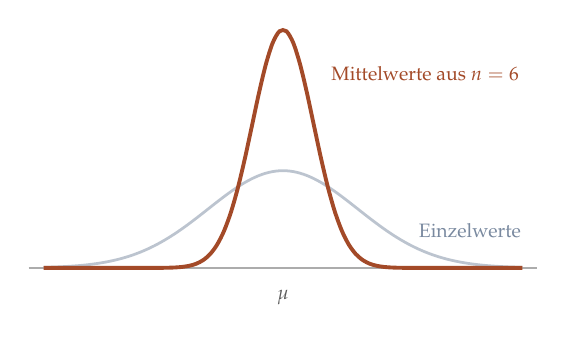
\begin{tikzpicture}[scale=0.95]
\draw[grau!50, line width=0.7pt] (-3.4,0) -- (3.4,0);
\draw[tief!30, line width=1.0pt, smooth, samples=70, domain=-3.2:3.2]
  plot (\x, {1.3*exp(-\x*\x/2)});
\draw[akzent, line width=1.4pt, smooth, samples=70, domain=-3.2:3.2]
  plot (\x, {1.3*2.449*exp(-6*\x*\x/2)});
\node[font=\scriptsize, color=tief!60] at (2.5,0.5) {Einzelwerte};
\node[font=\scriptsize, color=akzent] at (1.9,2.6) {Mittelwerte aus $n=6$};
\node[font=\scriptsize, color=grau] at (0,-0.4) {$\mu$};
\end{tikzpicture}
\end{center}

\begin{center}
\begin{minipage}{0.88\textwidth}
\kursiv{Man sieht die Behauptung schon im Bild: Die Mittelwerte streuen um denselben Punkt, aber \kursiv{enger}. Der folgende Satz sagt, um wie viel enger --- und die Antwort ist erstaunlich einfach.}
\end{minipage}
\end{center}
\end{merksatz}

\begin{merksatz}
\boxtitel{Satz 4.4 --- Erwartungswert und Varianz des Mittelwerts}
Seien $X_1, \ldots, X_n$ unabhängige Zufallsgrößen mit demselben Erwartungswert $\mu$ und derselben Varianz $\sigma^2$. Für $\overline{X} = \frac{1}{n}\sum_i X_i$ gilt
\[ \mathbb{E}[\overline{X}] = \mu, \qquad \Var[\overline{X}] = \frac{\sigma^2}{n} . \]
\end{merksatz}

\begin{merksatz}
\boxtitel{Beweis}
\schritt{Teil 1 --- der Erwartungswert}
\begin{align*}
\mathbb{E}[\overline X] &= \mathbb{E}\left[\frac{1}{n}\sum_{i=1}^n X_i\right]\\
&= \frac{1}{n}\,\mathbb{E}\left[\sum_{i=1}^n X_i\right] && \text{nach (R1) mit } a = \tfrac1n,\ b=0\\
&= \frac{1}{n}\sum_{i=1}^n \mathbb{E}[X_i] && \text{nach (R2), } n-1 \text{ mal angewandt}\\
&= \frac{1}{n}\sum_{i=1}^n \mu = \frac{1}{n}\cdot n\mu = \mu .
\end{align*}

\schritt{Was das bedeutet}
Der Stichprobenmittelwert ist \Begriff{erwartungstreu}: Im Durchschnitt über alle möglichen Stichproben trifft er den wahren Wert. Er ist im Einzelfall zu groß oder zu klein, aber nicht systematisch in eine Richtung verschoben.

Beachten Sie: Für diesen Teil wurde \kursiv{keine Unabhängigkeit} gebraucht --- (R2) gilt immer.

\schritt{Teil 2 --- die Varianz}
\begin{align*}
\Var[\overline X] &= \Var\left[\frac{1}{n}\sum_{i=1}^n X_i\right]\\
&= \frac{1}{n^2}\,\Var\left[\sum_{i=1}^n X_i\right] && \text{nach (R3), Quadrat des Faktors}\\
&= \frac{1}{n^2}\sum_{i=1}^n \Var[X_i] && \textcolor{akzent}{\text{nach (R4) --- hier wird Unabhängigkeit gebraucht}}\\
&= \frac{1}{n^2}\cdot n\sigma^2 = \frac{\sigma^2}{n} . \qquad \blacksquare
\end{align*}
\end{merksatz}

\begin{definition}
\boxtitelm{Definition 4.5 --- Standardfehler}
Die Standardabweichung der Stichprobenverteilung des Mittelwerts heißt \Begriff{Standardfehler}:
\[ \mathrm{SE} = \sqrt{\Var[\overline X]} = \frac{\sigma}{\sqrt n} . \]
Da $\sigma$ unbekannt ist, schätzt man ihn durch
\[ \widehat{\mathrm{SE}} = \frac{s}{\sqrt n} . \]
\end{definition}

\begin{warnung}
\boxtitelr{Standardabweichung und Standardfehler --- der versprochene Kasten}
\begin{center}
{\small
\renewcommand{\arraystretch}{1.55}
\begin{tabular}{@{}P{2.2cm}P{3.0cm}P{3.2cm}@{}}
\toprule
& \textbf{Standardabw. $s$} & \textbf{Standardfehler}\\
\midrule
Beschreibt & \textbf{die Daten} & \textbf{den Mittelwert}\\
Frage & Wie verschieden sind die Personen? & Wie genau kenne ich $\mu$?\\
Bei wachsendem $n$ & bleibt gleich & \textcolor{gruen}{wird kleiner}\\
Formel & --- & $s/\sqrt n$\\
\bottomrule
\end{tabular}}
\end{center}

\schritt{Die MOBIL-Gruppe B}
$s_B = 3{,}46$ Stunden bei $n = 6$:
\[ \widehat{\mathrm{SE}} = \frac{3{,}46}{\sqrt 6} = \frac{3{,}46}{2{,}449} = 1{,}41 \ \text{Stunden} . \]

\begin{center}
\renewcommand{\arraystretch}{1.45}
\begin{tabular}{@{}P{3.4cm}P{4.8cm}@{}}
\toprule
\enquote{$18{,}0 \pm 3{,}5$} & Die Personen streuen um etwa $3{,}5$ Stunden.\\
\enquote{$18{,}0 \pm 1{,}4$} & Der Mittelwert ist auf etwa $1{,}4$ Stunden genau bestimmt.\\
\bottomrule
\end{tabular}
\end{center}

\schritt{Was bei $n=60$ geschähe}
$s$ bliebe bei etwa $3{,}5$ --- die Personen werden nicht ähnlicher. Der Standardfehler fiele auf
\[ \frac{3{,}46}{\sqrt{60}} = \frac{3{,}46}{7{,}746} = 0{,}45 \ \text{Stunden} . \]

\begin{center}
\begin{minipage}{0.88\textwidth}
\kursiv{Wer in einer Abbildung Fehlerbalken zeigt, ohne zu sagen, welche Größe sie darstellen, macht die Abbildung unlesbar --- und im Zweifel sieht das Ergebnis mit Standardfehlern überzeugender aus. Bei $n=60$ ist der Unterschied fast das Achtfache.}
\end{minipage}
\end{center}
\end{warnung}

\begin{merksatz}
\boxtitel{Die Wurzel --- und was sie kostet}
Der Standardfehler fällt mit $1/\sqrt{n}$, nicht mit $1/n$. Das hat eine unbequeme Folge.

\begin{center}
\renewcommand{\arraystretch}{1.48}
\begin{tabular}{@{}P{2.8cm}P{2.4cm}P{2.6cm}@{}}
\toprule
\textbf{Genauigkeit} & \textbf{nötiges $n$} & \\
\midrule
Ausgangslage & $100$ & \\
doppelt so genau & $400$ & $4\times$ so viele\\
zehnmal so genau & $10\,000$ & $100\times$\\
\bottomrule
\end{tabular}
\end{center}

\schritt{Die Rechnung}
Aus $\frac{\sigma}{\sqrt{n_2}} = \frac{1}{2}\cdot\frac{\sigma}{\sqrt{n_1}}$ folgt $\sqrt{n_2} = 2\sqrt{n_1}$, also $n_2 = 4n_1$.

\begin{center}
\begin{minipage}{0.88\textwidth}
\kursiv{Das ist der Grund, warum große Studien so teuer sind und warum es einen Punkt gibt, ab dem sich Vergrößerung nicht mehr lohnt. Kapitel~7 macht daraus die Fallzahlplanung.}
\end{minipage}
\end{center}
\end{merksatz}

\section{Der zentrale Grenzwertsatz}

Satz 4.4 sagt, \kursiv{wo} die Mittelwerte liegen und wie weit sie streuen. Er sagt nichts über die \kursiv{Form} ihrer Verteilung. Das leistet der folgende Satz --- und er leistet etwas Erstaunliches.

\begin{merksatz}
\boxtitel{Satz 4.6 (Zentraler Grenzwertsatz)}
Seien $X_1, X_2, \ldots$ unabhängig, alle mit demselben Erwartungswert $\mu$ und derselben endlichen Varianz $\sigma^2 > 0$. Dann nähert sich die Verteilung von
\[ \frac{\overline{X} - \mu}{\sigma/\sqrt n} \]
mit wachsendem $n$ der Standardnormalverteilung --- \kursiv{unabhängig davon, wie die $X_i$ verteilt sind}.
\end{merksatz}

\begin{merksatz}
\boxtitel{Was daran erstaunlich ist}
\begin{center}
\begin{minipage}{0.9\textwidth}
Die Ausgangsverteilung darf schief sein, mehrgipflig, diskret, unsymmetrisch --- es ist gleichgültig. Die Mittelwerte werden trotzdem normalverteilt.
\end{minipage}
\end{center}

\begin{center}
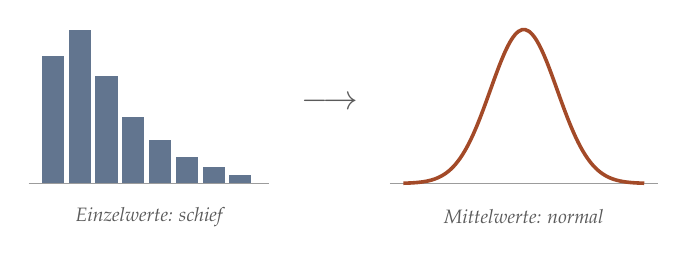
\begin{tikzpicture}[scale=0.85]
% links: schiefe Ausgangsverteilung
\begin{scope}
\draw[grau!60, line width=0.6pt] (0,0) -- (3.6,0);
\foreach \x/\h in {0.2/1.9, 0.6/2.3, 1.0/1.6, 1.4/1.0, 1.8/0.65, 2.2/0.4, 2.6/0.25, 3.0/0.12}
  \fill[tief!70] (\x,0) rectangle (\x+0.33,\h);
\node[font=\scriptsize\itshape, color=grau] at (1.8,-0.5) {Einzelwerte: schief};
\end{scope}
\node[font=\large, color=grau] at (4.5,1.2) {$\longrightarrow$};
% rechts: normal
\begin{scope}[xshift=5.6cm]
\draw[grau!60, line width=0.6pt] (-0.2,0) -- (3.8,0);
\draw[akzent, line width=1.3pt, smooth, samples=70, domain=0:3.6]
  plot (\x, {2.3*exp(-(\x-1.8)*(\x-1.8)/0.5)});
\node[font=\scriptsize\itshape, color=grau] at (1.8,-0.5) {Mittelwerte: normal};
\end{scope}
\end{tikzpicture}
\end{center}

\schritt{Warum das die Statistik überhaupt möglich macht}
Ohne diesen Satz müsste man für jede Fragestellung die Verteilung der Einzelwerte kennen --- und die kennt man fast nie. Der Satz erlaubt, mit einer einzigen Verteilung zu arbeiten, gleichgültig woher die Daten kommen.
\end{merksatz}

\begin{warnung}
\boxtitelr{Vier Dinge, die der Satz nicht sagt}
\begin{center}
\renewcommand{\arraystretch}{1.55}
\begin{tabular}{@{}P{1.0cm}P{7.4cm}@{}}
\toprule
$1$ & \textbf{Nicht: Die Daten werden normalverteilt.} Die Einzelwerte bleiben, wie sie sind. Nur die \kursiv{Mittelwerte} werden normal.\\
$2$ & \textbf{Nicht: Das gilt ab $n = 30$.} Diese Faustregel steht in vielen Büchern und hat keine theoretische Grundlage. Bei stark schiefen Verteilungen braucht man Hunderte, bei symmetrischen genügen oft fünf.\\
$3$ & \textbf{Nicht: Bei genügend großem $n$ ist alles in Ordnung.} Der Satz setzt Unabhängigkeit und endliche Varianz voraus. Fehlt eines, gilt er nicht --- auch bei $n = 10^6$ nicht.\\
$4$ & \textbf{Nicht: Die Ränder stimmen auch.} Die Annäherung ist in der Mitte gut und an den äußeren Rändern schlecht. Für sehr kleine $p$-Werte ist sie unzuverlässig.\\
\bottomrule
\end{tabular}
\end{center}

\schritt{Zu Punkt 3 --- ein Beispiel}
Misst man denselben Menschen zehnmal, so sind die Werte nicht unabhängig. Man hat dann nicht $n=10$, sondern näherungsweise $n=1$ mit zehn Wiederholungen. Wer trotzdem durch $\sqrt{10}$ teilt, unterschätzt den Standardfehler um den Faktor drei.

\begin{center}
\begin{minipage}{0.88\textwidth}
\kursiv{Dieser Fehler --- \Begriff{Pseudoreplikation} --- ist in der medizinischen Literatur verbreitet: mehrere Messungen je Person, mehrere Zähne je Gebiss, mehrere Augen je Kopf. Die richtige Behandlung leistet die Mehrebenenmodellierung; Kapitel~11 deutet sie an.}
\end{minipage}
\end{center}
\end{warnung}

\section{Übungsaufgaben}

\begin{aufgabe}
\boxtitel{Aufgabe 4.1 --- Rechnen mit der Normalverteilung}
Die Mobilisationszeit nach dem bisherigen Schema sei normalverteilt mit $\mu = 26$ Stunden und $\sigma = 6$ Stunden.
\begin{center}
{\small
\renewcommand{\arraystretch}{1.35}
\begin{tabular}{@{}P{4.2cm}P{4.2cm}@{}}
\toprule
(a) Anteil unter $20$ Stunden? & (c) Welche Zeit unterschreiten $90\,\%$?\\
(b) Anteil zwischen $20$ und $32$? & (d) Anteil über $40$ Stunden?\\
\bottomrule
\end{tabular}}
\end{center}

\loesung
\schritt{(a) --- Standardisieren}
\[ z = \frac{20 - 26}{6} = \frac{-6}{6} = -1{,}00 \]
\[ \Pr[X < 20] = \Phi(-1{,}00) = 1 - \Phi(1{,}00) = 1 - 0{,}8413 = \mathbf{0{,}1587} . \]
Etwa $15{,}9\,\%$.

\schritt{(b) --- Zwei Grenzen}
\[ z_1 = \frac{20-26}{6} = -1{,}00, \qquad z_2 = \frac{32-26}{6} = +1{,}00 \]
\[ \Pr[20 \le X \le 32] = \Phi(1{,}00) - \Phi(-1{,}00) = 0{,}8413 - 0{,}1587 = \mathbf{0{,}6826} . \]
Das ist die $68$-Prozent-Regel --- die Grenzen liegen genau bei $\mu \pm 1\sigma$. \checkmark

\schritt{(c) --- Rückwärts rechnen}
Gesucht ist $x$ mit $\Phi\!\left(\frac{x-26}{6}\right) = 0{,}90$.

Aus der Tabelle: $\Phi(1{,}28) = 0{,}8997 \approx 0{,}90$. Also
\[ \frac{x - 26}{6} = 1{,}28 \quad\Longrightarrow\quad x = 26 + 6 \cdot 1{,}28 = 26 + 7{,}68 = \mathbf{33{,}7} \ \text{Stunden} . \]

\schritt{(d) --- Der Rand}
\[ z = \frac{40-26}{6} = \frac{14}{6} = 2{,}333 \]
Die Tabelle gibt $\Phi(2{,}33) \approx 0{,}9901$, also
\[ \Pr[X > 40] = 1 - 0{,}9901 = \mathbf{0{,}0099} \approx 1\,\% . \]

\schritt{Die Probe --- und ein Vorbehalt}
Alle vier Ergebnisse sind plausibel. Aber: Die Annahme der Normalverteilung ist hier fragwürdig.

Eine normalverteilte Größe kann beliebig kleine Werte annehmen. Für $\mu=26$, $\sigma=6$ wäre
\[ \Pr[X < 0] = \Phi\!\left(\frac{0-26}{6}\right) = \Phi(-4{,}33) \approx 0{,}000008 . \]
Das ist winzig, aber nicht null --- und eine negative Mobilisationszeit gibt es nicht.

\begin{center}
\begin{minipage}{0.86\textwidth}
\kursiv{Bei Zeitdauern ist die Normalverteilung stets nur eine Näherung. Sie ist brauchbar, solange $\mu$ mehrere Standardabweichungen über null liegt --- hier gut vier. Bei $\mu = 10$ und $\sigma = 6$ wäre sie es nicht mehr, und man nähme eine Verteilung, die nur positive Werte zulässt.}
\end{minipage}
\end{center}
\end{aufgabe}

\begin{aufgabe}
\boxtitel{Aufgabe 4.2 --- Standardfehler und Fallzahl}
Bei der MOBIL-Studie soll der Mittelwert der Gruppe B auf $\pm 0{,}5$ Stunden genau bestimmt werden --- gemeint ist ein Standardfehler von höchstens $0{,}5$. Wie viele Personen braucht man, wenn $\sigma \approx 3{,}5$ Stunden ist?

\loesung
\schritt{Schritt 1 --- Die Bedingung aufschreiben}
\[ \frac{\sigma}{\sqrt n} \le 0{,}5 \]

\schritt{Schritt 2 --- Nach $n$ auflösen}
\begin{align*}
\frac{3{,}5}{\sqrt n} &\le 0{,}5\\
3{,}5 &\le 0{,}5\sqrt n\\
\sqrt n &\ge \frac{3{,}5}{0{,}5} = 7\\
n &\ge 49 .
\end{align*}

\schritt{Antwort}
Mindestens $\mathbf{49}$ Personen in der Gruppe.

\schritt{Probe}
\[ \frac{3{,}5}{\sqrt{49}} = \frac{3{,}5}{7} = 0{,}50 . \quad \checkmark \]

\schritt{Schritt 3 --- Was die Studie tatsächlich vorsieht}
Die MOBIL-Studie hat $n = 60$ je Gruppe:
\[ \mathrm{SE} = \frac{3{,}5}{\sqrt{60}} = \frac{3{,}5}{7{,}746} = 0{,}452 \ \text{Stunden} . \]
Die geplante Genauigkeit wird erreicht. \checkmark

\schritt{Schritt 4 --- Was doppelte Genauigkeit kostete}
Für $\mathrm{SE} \le 0{,}25$:
\[ \sqrt n \ge \frac{3{,}5}{0{,}25} = 14 \quad\Longrightarrow\quad n \ge 196 . \]
Viermal so viele Personen für die halbe Unsicherheit --- die Wurzelregel in Zahlen.

\schritt{Nachbemerkung}
Diese Rechnung ist noch keine Fallzahlplanung. Sie fragt nach der \kursiv{Genauigkeit einer Schätzung}, nicht nach der Fähigkeit, einen Unterschied nachzuweisen. Letzteres verlangt zusätzlich eine Vorstellung davon, wie groß der Unterschied sein könnte --- Kapitel~7.
\end{aufgabe}

\begin{aufgabe}
\boxtitel{Aufgabe 4.3 --- Der Grenzwertsatz an einem Würfel}
Ein Würfel liefert die Augenzahlen $1$ bis $6$ mit gleicher Wahrscheinlichkeit.
\begin{center}
{\small
\renewcommand{\arraystretch}{1.35}
\begin{tabular}{@{}P{4.2cm}P{4.2cm}@{}}
\toprule
(a) $\mu$ und $\sigma$ bestimmen & (c) Wahrscheinlichkeit, dass\\
(b) Verteilung von $\overline X$ für $n=36$ & \quad $\overline X > 4$?\\
\bottomrule
\end{tabular}}
\end{center}

\loesung
\schritt{(a) --- Erwartungswert}
Jede Augenzahl hat Wahrscheinlichkeit $\frac16$:
\[ \mu = \frac{1+2+3+4+5+6}{6} = \frac{21}{6} = 3{,}5 . \]

\schritt{Varianz über den Verschiebungssatz}
\[ \mathbb{E}[X^2] = \frac{1+4+9+16+25+36}{6} = \frac{91}{6} \approx 15{,}167 \]
\[ \sigma^2 = \mathbb{E}[X^2] - \mu^2 = 15{,}167 - 12{,}25 = 2{,}917 \]
\[ \sigma = \sqrt{2{,}917} \approx 1{,}708 . \]

\schritt{(b) --- Die Stichprobenverteilung}
Nach Satz 4.4:
\[ \mathbb{E}[\overline X] = 3{,}5, \qquad \Var[\overline X] = \frac{2{,}917}{36} = 0{,}0810 , \]
\[ \mathrm{SE} = \sqrt{0{,}0810} = 0{,}2847 . \]

Nach Satz 4.6 ist $\overline X$ näherungsweise $\mathcal{N}(3{,}5;\ 0{,}0810)$ verteilt.

\schritt{(c) --- Die gesuchte Wahrscheinlichkeit}
\[ z = \frac{4 - 3{,}5}{0{,}2847} = \frac{0{,}5}{0{,}2847} = 1{,}756 \]
Die Tabelle: $\Phi(1{,}76) \approx 0{,}9608$. Also
\[ \Pr[\overline X > 4] \approx 1 - 0{,}9608 = \mathbf{0{,}039} , \]
etwa $3{,}9\,\%$.

\schritt{Die Deutung}
Die Einzelverteilung des Würfels ist \kursiv{gleichverteilt} --- ein Rechteck, nichts weniger glockenförmig lässt sich denken. Trotzdem ist der Mittelwert aus $36$ Würfen sehr gut normalverteilt; die Näherung stimmt hier auf zwei Stellen.

\begin{center}
\begin{minipage}{0.86\textwidth}
\kursiv{Das ist der Grund, warum die Faustregel \enquote{ab $n=30$} überhaupt entstanden ist: Bei symmetrischen Ausgangsverteilungen stimmt sie sogar für viel kleinere $n$. Bei schiefen --- etwa Wartezeiten --- versagt sie. Die Faustregel beschreibt den bequemen Fall und wird auf alle Fälle angewandt.}
\end{minipage}
\end{center}

\schritt{Zum Vergleich --- die Einzelbeobachtung}
Wie wahrscheinlich ist es, dass ein \kursiv{einzelner} Wurf über $4$ liegt? Das sind die Augenzahlen $5$ und $6$:
\[ \frac{2}{6} = 0{,}333 . \]
Gegen $0{,}039$ beim Mittelwert aus $36$ Würfen --- fast das Zehnfache. Genau das leistet die Mittelung: Extreme werden unwahrscheinlich.
\end{aufgabe}

\begin{geschichte}
\boxtitelg{Drei Jahrhunderte für einen Satz}
Der zentrale Grenzwertsatz hat eine ungewöhnlich lange Entstehungsgeschichte.

\begin{center}
{\small
\renewcommand{\arraystretch}{1.42}
\begin{tabular}{@{}P{1.6cm}P{2.2cm}P{4.0cm}@{}}
\toprule
\textbf{Jahr} & \textbf{Person} & \textbf{Beitrag}\\
\midrule
$1733$ & de Moivre & Der Fall der Münzwürfe\\
$1809$ & Gauß & Die Normalverteilung als Fehlergesetz\\
$1810$ & Laplace & Verallgemeinerung auf beliebige Verteilungen\\
$1901$ & Ljapunow & Erster strenger Beweis\\
$1920$ & Pólya & Der Name \enquote{zentraler Grenzwertsatz}\\
$1922$ & Lindeberg & Die heute übliche Bedingung\\
\bottomrule
\end{tabular}}
\end{center}

\Person{Abraham de Moivre} fand 1733 als Erster die Glockenkurve --- als Näherung für die Binomialverteilung bei vielen Münzwürfen. Er veröffentlichte das Ergebnis auf sieben Seiten, lateinisch, im Selbstverlag, und es blieb weitgehend unbeachtet.

\begin{center}
\begin{minipage}{0.9\textwidth}
\kursiv{Der Name ist ein Übersetzungsproblem. Pólya nannte den Satz \enquote{zentral} im Sinne von \enquote{von zentraler Bedeutung für die Wahrscheinlichkeitstheorie}. Im Deutschen liest man es leicht als \enquote{Satz über den zentralen Grenzwert}, was keinen Sinn ergibt. Im Englischen besteht dieselbe Zweideutigkeit.}
\end{minipage}
\end{center}

\Person{Carl Friedrich Gauß} begründete die Normalverteilung 1809 ganz anders: Er fragte, für welches Fehlergesetz das arithmetische Mittel der beste Schätzer wäre --- und rechnete rückwärts zur Glockenkurve. Die Kurve ist also nicht aus den Daten gefunden, sondern aus dem Wunsch, mitteln zu dürfen.
\end{geschichte}

\begin{forschung}
\boxtitelp{Wie groß muss $n$ sein?}
Die Frage hat keine allgemeine Antwort, und die Faustregel \enquote{$n \ge 30$} ist nicht haltbar.

\begin{center}
{\small
\renewcommand{\arraystretch}{1.45}
\begin{tabular}{@{}P{3.2cm}P{2.2cm}P{2.8cm}@{}}
\toprule
\textbf{Ausgangs\-verteilung} & \textbf{nötiges $n$} & \\
\midrule
symmetrisch, eingipflig & $\approx 5$ & \textcolor{gruen}{sehr schnell}\\
gleichverteilt & $\approx 12$ & \textcolor{gruen}{schnell}\\
mäßig schief & $\approx 30$ & die Faustregel\\
stark schief (Lognormal) & $\approx 100$ bis $300$ & \textcolor{akzent}{deutlich mehr}\\
sehr schwere Ränder & \textcolor{akzent}{gar nicht} & \textcolor{akzent}{\textbf{Varianz unendlich}}\\
\bottomrule
\end{tabular}}
\end{center}

Die letzte Zeile betrifft Verteilungen ohne endliche Varianz --- die bekannteste ist die Cauchy-Verteilung. Bei ihr ist der Mittelwert aus $n$ Beobachtungen genauso gestreut wie eine Einzelbeobachtung, gleichgültig wie groß $n$ wird. Mitteln hilft dort überhaupt nicht.

\begin{center}
\begin{minipage}{0.88\textwidth}
\kursiv{In der Medizin trifft man solche Fälle bei Kostendaten und Liegedauern: wenige extreme Werte tragen den Großteil der Summe. Dort arbeitet man mit Medianen, mit logarithmierten Werten oder mit verteilungsfreien Verfahren --- Kapitel~9.}
\end{minipage}
\end{center}

Praktisch prüft man die Annahme nicht durch Rechnen an der Faustregel, sondern durch \Begriff{Simulation}: Man zieht wiederholt Stichproben aus einer Verteilung, die den Daten ähnelt, und sieht nach, ob die Mittelwerte normal aussehen. Das ist der Bootstrap-Gedanke aus Kapitel~9.
\end{forschung}

\begin{merksatz}
\boxtitel{Was Sie jetzt können}
\begin{center}
\renewcommand{\arraystretch}{1.5}
\begin{tabular}{@{}P{3.2cm}P{5.4cm}@{}}
\toprule
\textbf{Definition 4.1} & Parameter fest und unbekannt, Schätzer bekannt und zufällig\\
\textbf{Normal\-verteilung} & Standardisieren, Tabelle, die Zahl $1{,}96$\\
\textbf{Satz 4.4} & $\mathbb{E}[\overline X] = \mu$ und $\Var[\overline X] = \sigma^2/n$\\
\textbf{Definition 4.5} & Standardfehler --- und der Unterschied zu $s$\\
\textbf{Satz 4.6} & Zentraler Grenzwertsatz --- und vier Dinge, die er nicht sagt\\
\bottomrule
\end{tabular}
\end{center}

\begin{center}
\begin{minipage}{0.88\textwidth}
\kursiv{Im nächsten Kapitel fragen wir, was einen Schätzer gut macht --- und lösen dabei das in Kapitel~2 vertagte Rätsel des $n-1$.}
\end{minipage}
\end{center}
\end{merksatz}

\chapter{Punktschätzer und ihre Güte}

\section{Was ein Schätzer ist}

\begin{definition}
\boxtitelm{Definition 5.1 --- Schätzer}
Ein \Begriff{Schätzer} für einen Parameter $\theta$ ist eine Vorschrift, die aus den Daten $X_1,\ldots,X_n$ eine Zahl $\hat\theta$ berechnet.

Da die Daten zufällig sind, ist $\hat\theta$ eine Zufallsgröße --- sie hat eine Verteilung, einen Erwartungswert und eine Varianz.
\end{definition}

\begin{merksatz}
\boxtitel{Es gibt immer mehrere}
Für den Mittelwert einer Grundgesamtheit kommen alle folgenden Vorschriften infrage:

\begin{center}
{\small
\renewcommand{\arraystretch}{1.5}
\begin{tabular}{@{}P{3.4cm}P{5.0cm}@{}}
\toprule
$\MW$ & das arithmetische Mittel\\
$\Med$ & der Median\\
$\frac{x_{(1)}+x_{(n)}}{2}$ & die Mitte zwischen kleinstem und größtem Wert\\
$x_1$ & einfach die erste Beobachtung\\
$\mathbf{42}$ & eine feste Zahl, ohne Ansehen der Daten\\
\bottomrule
\end{tabular}}
\end{center}

Alle fünf sind Schätzer im Sinne der Definition. Die Frage ist, was sie unterscheidet --- und dafür braucht man Gütekriterien.

\begin{center}
\begin{minipage}{0.88\textwidth}
\kursiv{Die letzte Zeile ist nicht als Scherz gemeint. Sie hat Varianz null und ist, falls $\mu$ zufällig $42$ beträgt, der beste Schätzer überhaupt. Andernfalls ist sie unbrauchbar. Ein Gütekriterium muss beides erfassen können.}
\end{minipage}
\end{center}
\end{merksatz}

\section{Erwartungstreue}

\begin{definition}
\boxtitelm{Definition 5.2 --- Erwartungstreue und Verzerrung}
Ein Schätzer heißt \Begriff{erwartungstreu}, wenn
\[ \mathbb{E}[\hat\theta] = \theta \]
für jeden möglichen Wert von $\theta$ gilt. Die Größe
\[ \mathrm{Bias}(\hat\theta) = \mathbb{E}[\hat\theta] - \theta \]
heißt \Begriff{Verzerrung}.
\end{definition}

\begin{merksatz}
\boxtitel{Was das heißt und was nicht}
\begin{center}
\renewcommand{\arraystretch}{1.55}
\begin{tabular}{@{}P{2.4cm}P{6.2cm}@{}}
\toprule
\textbf{Es heißt} & Wiederholte man die Studie unendlich oft, so träfe der Durchschnitt aller Schätzwerte den wahren Wert.\\
\textbf{Es heißt nicht} & dass der Schätzer in \kursiv{dieser} Studie richtig liegt. Er kann beliebig weit daneben sein.\\
\bottomrule
\end{tabular}
\end{center}

\begin{center}
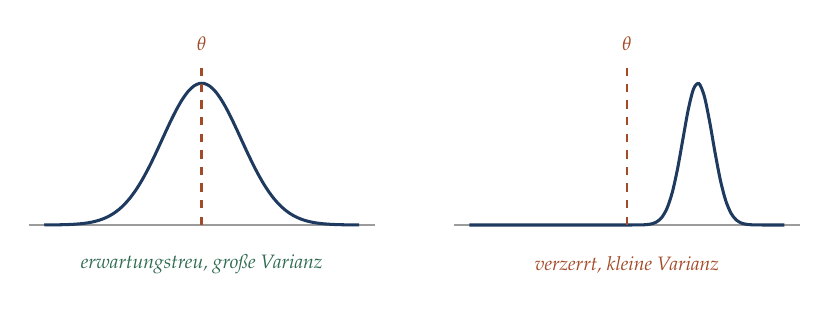
\begin{tikzpicture}[scale=1.0]
\begin{scope}
\draw[grau!60, line width=0.6pt] (-2.2,0) -- (2.2,0);
\draw[tief, line width=1.1pt, smooth, samples=60, domain=-2:2] plot (\x, {1.8*exp(-\x*\x*2)});
\draw[akzent, dashed, line width=0.9pt] (0,0) -- (0,2.0);
\node[font=\scriptsize, color=akzent] at (0,2.3) {$\theta$};
\node[font=\scriptsize\itshape, color=gruen] at (0,-0.5) {erwartungstreu, große Varianz};
\end{scope}
\begin{scope}[xshift=5.4cm]
\draw[grau!60, line width=0.6pt] (-2.2,0) -- (2.2,0);
\draw[tief, line width=1.1pt, smooth, samples=60, domain=-2:2] plot (\x, {1.8*exp(-(\x-0.9)*(\x-0.9)*14)});
\draw[akzent, dashed, line width=0.9pt] (0,0) -- (0,2.0);
\node[font=\scriptsize, color=akzent] at (0,2.3) {$\theta$};
\node[font=\scriptsize\itshape, color=akzent] at (0,-0.5) {verzerrt, kleine Varianz};
\end{scope}
\end{tikzpicture}
\end{center}

\begin{center}
\begin{minipage}{0.88\textwidth}
\kursiv{Welcher der beiden ist besser? Das lässt sich noch nicht entscheiden --- man braucht ein Kriterium, das Verzerrung und Streuung gemeinsam bewertet. Abschnitt 5.5 liefert es.}
\end{minipage}
\end{center}
\end{merksatz}

\section{Warum $n-1$ --- die Einlösung}

Wir holen nun nach, was Kapitel~2 vertagt hat.

\begin{merksatz}
\boxtitel{Ein Hilfssatz, den wir zweimal brauchen}
Für jede Zufallsgröße $X$ mit $\mathbb{E}[X] = \mu$ gilt
\[ \mathbb{E}[X^2] = \Var[X] + \mu^2 . \]

\schritt{Beweis}
\begin{align*}
\Var[X] &= \mathbb{E}\bigl[(X-\mu)^2\bigr] && \text{Definition}\\
&= \mathbb{E}\bigl[X^2 - 2\mu X + \mu^2\bigr]\\
&= \mathbb{E}[X^2] - 2\mu\,\mathbb{E}[X] + \mu^2 && \text{nach (R1) und (R2)}\\
&= \mathbb{E}[X^2] - 2\mu^2 + \mu^2 = \mathbb{E}[X^2] - \mu^2 .
\end{align*}
Umstellen ergibt die Behauptung. $\blacksquare$

\begin{center}
\begin{minipage}{0.88\textwidth}
\kursiv{Das ist der Verschiebungssatz aus Kapitel~2 --- nur für Zufallsgrößen statt für Datenreihen. Dieselbe Rechnung, andere Bühne.}
\end{minipage}
\end{center}
\end{merksatz}

\begin{merksatz}
\boxtitel{Satz 5.3 --- Die Stichprobenvarianz ist erwartungstreu}
Seien $X_1,\ldots,X_n$ unabhängig mit Erwartungswert $\mu$ und Varianz $\sigma^2$. Dann gilt für
\[ S^2 = \frac{1}{n-1}\sum_{i=1}^n (X_i - \overline X)^2 \]
die Gleichung $\mathbb{E}[S^2] = \sigma^2$.
\end{merksatz}

\begin{merksatz}
\boxtitel{Beweis --- in fünf Schritten}
\schritt{Schritt 1 --- Den Verschiebungssatz anwenden}
Nach Satz 2.11 gilt für jede Datenreihe
\[ \sum_{i=1}^n (X_i - \overline X)^2 = \sum_{i=1}^n X_i^2 - n\,\overline X^2 . \]
Das ist eine algebraische Identität und gilt daher auch für Zufallsgrößen.

\schritt{Schritt 2 --- Erwartungswert bilden}
\[ \mathbb{E}\left[\sum_i (X_i-\overline X)^2\right] = \sum_{i=1}^n \mathbb{E}[X_i^2] \;-\; n\,\mathbb{E}[\overline X^2] . \]
Hier wurde (R2) benutzt --- die Summenregel für Erwartungswerte, die immer gilt.

\schritt{Schritt 3 --- Den ersten Term ausrechnen}
Nach dem Hilfssatz, angewandt auf $X_i$:
\[ \mathbb{E}[X_i^2] = \Var[X_i] + \mu^2 = \sigma^2 + \mu^2 . \]
Da das für jedes $i$ gilt:
\[ \sum_{i=1}^n \mathbb{E}[X_i^2] = n\,(\sigma^2 + \mu^2) . \]

\schritt{Schritt 4 --- Den zweiten Term ausrechnen}
Nun der entscheidende Schritt. Wir wenden den Hilfssatz auf $\overline X$ an:
\[ \mathbb{E}[\overline X^2] = \Var[\overline X] + \bigl(\mathbb{E}[\overline X]\bigr)^2 . \]
Nach Satz 4.4 ist $\Var[\overline X] = \sigma^2/n$ und $\mathbb{E}[\overline X] = \mu$. Also
\[ \mathbb{E}[\overline X^2] = \frac{\sigma^2}{n} + \mu^2 . \]

\schritt{Schritt 5 --- Zusammensetzen}
\begin{align*}
\mathbb{E}\left[\sum_i (X_i-\overline X)^2\right] &= n(\sigma^2+\mu^2) \;-\; n\left(\frac{\sigma^2}{n} + \mu^2\right)\\
&= n\sigma^2 + n\mu^2 - \sigma^2 - n\mu^2\\
&= (n-1)\,\sigma^2 .
\end{align*}

Teilt man beide Seiten durch $n-1$, so steht links $\mathbb{E}[S^2]$ und rechts $\sigma^2$. $\blacksquare$
\end{merksatz}

\begin{merksatz}
\boxtitel{Was der Beweis inhaltlich sagt}
\begin{center}
\begin{minipage}{0.9\textwidth}
Teilte man durch $n$, so bekäme man im Mittel
\[ \frac{(n-1)\sigma^2}{n} = \sigma^2 \cdot \frac{n-1}{n} \;<\; \sigma^2 . \]
Der Schätzer wäre also \kursiv{systematisch zu klein}, und zwar um den Faktor $\frac{n-1}{n}$.
\end{minipage}
\end{center}

\begin{center}
\renewcommand{\arraystretch}{1.45}
\begin{tabular}{@{}P{1.6cm}P{2.4cm}P{3.0cm}@{}}
\toprule
$n$ & $\frac{n-1}{n}$ & \textbf{Unterschätzung}\\
\midrule
$2$ & $0{,}500$ & \textcolor{akzent}{um die Hälfte}\\
$6$ & $0{,}833$ & um $17\,\%$\\
$30$ & $0{,}967$ & um $3\,\%$\\
$1000$ & $0{,}999$ & belanglos\\
\bottomrule
\end{tabular}
\end{center}

\schritt{Die anschauliche Begründung}
Nach Satz 2.4 minimiert der Mittelwert die Summe der quadratischen Abweichungen. Der \kursiv{Stichproben}mittelwert $\overline X$ liegt also näher an den Daten als der wahre Wert $\mu$ --- er wurde ja aus genau diesen Daten so gewählt.

Misst man die Abweichungen von $\overline X$ statt von $\mu$, so bekommt man daher zu kleine Werte. Der Faktor $\frac{n}{n-1}$ gleicht das aus.

\begin{center}
\begin{minipage}{0.88\textwidth}
\kursiv{Der Verlust beträgt genau \enquote{einen Freiheitsgrad}: Aus $n$ Beobachtungen wurde ein Parameter geschätzt, also bleiben $n-1$ unabhängige Abweichungen übrig. Satz 2.3 sagt das direkt --- die Abweichungen summieren sich zu null, also legt die letzte sich aus den ersten $n-1$ fest.}
\end{minipage}
\end{center}
\end{merksatz}

\begin{warnung}
\boxtitelr{Und trotzdem ist $s$ nicht erwartungstreu}
Satz 5.3 gilt für die Varianz $S^2$, nicht für die Standardabweichung $S$.

Aus $\mathbb{E}[S^2] = \sigma^2$ folgt \kursiv{nicht} $\mathbb{E}[S] = \sigma$. Die Wurzel ist keine lineare Funktion, und Erwartungswerte vertauschen nicht mit nichtlinearen Funktionen.

Tatsächlich gilt $\mathbb{E}[S] < \sigma$ --- die Standardabweichung wird stets etwas unterschätzt. Bei $n=6$ und Normalverteilung beträgt der Fehler etwa $5\,\%$.

\begin{center}
\begin{minipage}{0.88\textwidth}
\kursiv{Man korrigiert das in der Praxis nicht, weil die Korrektur von der Verteilung abhängt und der Fehler bei brauchbaren Stichprobenumfängen klein ist. Aber man sollte wissen, dass die vertraute Formel diese Eigenschaft nicht hat --- \enquote{erwartungstreu} gilt für $s^2$, nicht für $s$.}
\end{minipage}
\end{center}
\end{warnung}

\section{Konsistenz}

\begin{definition}
\boxtitelm{Definition 5.4}
Ein Schätzer heißt \Begriff{konsistent}, wenn er sich mit wachsendem Stichprobenumfang dem wahren Wert beliebig nähert --- genauer: wenn für jedes $\varepsilon > 0$
\[ \Pr\bigl[\,|\hat\theta_n - \theta| > \varepsilon\,\bigr] \;\longrightarrow\; 0 \quad \text{für } n \to \infty . \]
\end{definition}

\begin{merksatz}
\boxtitel{Warum $\MW$ konsistent ist}
Nach Satz 4.4 ist $\Var[\overline X] = \sigma^2/n \to 0$, und der Erwartungswert ist stets $\mu$.

Eine Zufallsgröße, deren Erwartungswert der Zielwert ist und deren Streuung gegen null geht, muss sich dem Zielwert nähern. Streng begründet wird das mit der Tschebyschew-Ungleichung (Band 4, Kapitel 7):
\[ \Pr\bigl[|\overline X - \mu| > \varepsilon\bigr] \;\le\; \frac{\Var[\overline X]}{\varepsilon^2} = \frac{\sigma^2}{n\varepsilon^2} \;\longrightarrow\; 0 . \]
\end{merksatz}

\begin{warnung}
\boxtitelr{Die beiden Eigenschaften sind unabhängig voneinander}
\begin{center}
{\small
\renewcommand{\arraystretch}{1.5}
\begin{tabular}{@{}P{2.8cm}P{2.4cm}P{2.6cm}@{}}
\toprule
\textbf{Schätzer für $\mu$} & \textbf{erwartungstreu} & \textbf{konsistent}\\
\midrule
$\overline X$ & \textcolor{gruen}{ja} & \textcolor{gruen}{ja}\\
$X_1$ (erste Beob.) & \textcolor{gruen}{\textbf{ja}} & \textcolor{akzent}{\textbf{nein}}\\
$\overline X + \frac{1}{n}$ & \textcolor{akzent}{nein} & \textcolor{gruen}{ja}\\
Die Zahl $42$ & \textcolor{akzent}{nein} & \textcolor{akzent}{nein}\\
\bottomrule
\end{tabular}}
\end{center}

\schritt{Die zweite Zeile erklärt}
$X_1$ ist erwartungstreu: $\mathbb{E}[X_1] = \mu$ nach Voraussetzung. Aber die Varianz bleibt $\sigma^2$, gleichgültig wie groß $n$ wird --- man wirft ja alle übrigen Daten weg. Der Schätzer wird nie genauer.

\begin{center}
\begin{minipage}{0.88\textwidth}
\kursiv{Das zeigt, dass Erwartungstreue allein nichts wert ist. Sie ist eine Aussage über den Mittelwert unendlich vieler gedachter Wiederholungen und sagt nichts über die Genauigkeit im Einzelfall.}
\end{minipage}
\end{center}
\end{warnung}

\section{Der mittlere quadratische Fehler}

\begin{definition}
\boxtitelm{Definition 5.5}
\[ \mathrm{MSE}(\hat\theta) = \mathbb{E}\bigl[(\hat\theta - \theta)^2\bigr] . \]
\end{definition}

\begin{merksatz}
\boxtitel{Satz 5.6 --- Die Zerlegung}
\[ \mathrm{MSE}(\hat\theta) = \Var[\hat\theta] \;+\; \bigl(\mathrm{Bias}(\hat\theta)\bigr)^2 . \]

\schritt{Beweis}
Wir schreiben $b = \mathbb{E}[\hat\theta]$ und fügen eine Null ein:
\begin{align*}
\mathbb{E}\bigl[(\hat\theta-\theta)^2\bigr] &= \mathbb{E}\bigl[\bigl((\hat\theta - b) + (b - \theta)\bigr)^2\bigr]\\
&= \mathbb{E}\bigl[(\hat\theta-b)^2\bigr] + 2(b-\theta)\,\mathbb{E}[\hat\theta - b] + (b-\theta)^2 .
\end{align*}
Der mittlere Term verschwindet, denn $\mathbb{E}[\hat\theta - b] = b - b = 0$. Der erste ist $\Var[\hat\theta]$, der letzte ist das Quadrat der Verzerrung. $\blacksquare$

\begin{center}
\begin{minipage}{0.88\textwidth}
\kursiv{Es ist derselbe Kniff wie in Satz 2.4 --- eine Null einfügen, ausquadrieren, der Mischterm fällt weg. Diese Figur kommt in der Statistik so oft vor, dass sie ein eigenes Gesicht verdient.}
\end{minipage}
\end{center}
\end{merksatz}

\begin{merksatz}
\boxtitel{Wann ein verzerrter Schätzer besser ist}
Satz 5.6 macht sichtbar, dass sich Verzerrung und Varianz gegeneinander aufrechnen lassen. Ein wenig Verzerrung kann sich lohnen, wenn sie viel Varianz spart.

\schritt{Ein Beispiel}
Wir schätzen $\sigma^2$ mit dem Faktor $\frac{1}{n+1}$ statt $\frac{1}{n-1}$. Bei normalverteilten Daten ergibt sich:

\begin{center}
{\small
\renewcommand{\arraystretch}{1.5}
\begin{tabular}{@{}P{2.4cm}P{2.2cm}P{2.2cm}P{1.6cm}@{}}
\toprule
\textbf{Teiler} & \textbf{Bias} & \textbf{Varianz} & \textbf{MSE}\\
\midrule
$n-1$ & $0$ & $\frac{2\sigma^4}{n-1}$ & $\frac{2\sigma^4}{n-1}$\\[3pt]
$n$ & klein & kleiner & kleiner\\[3pt]
$\mathbf{n+1}$ & \textcolor{akzent}{größer} & \textcolor{gruen}{am kleinsten} & \textcolor{gruen}{\textbf{minimal}}\\
\bottomrule
\end{tabular}}
\end{center}

Der Teiler $n+1$ liefert den kleinsten mittleren quadratischen Fehler --- und wird trotzdem nirgends verwendet.

\begin{center}
\begin{minipage}{0.88\textwidth}
\kursiv{Warum nicht? Weil die Rechnung die Normalverteilung voraussetzt, weil die Erwartungstreue bei der Weiterverarbeitung --- etwa in der Varianzanalyse --- gebraucht wird, und weil die Einheitlichkeit der Literatur einen Wert hat. Es ist eine Konvention, und sie ist nicht in jedem Sinn optimal. Das sollte man wissen.}
\end{minipage}
\end{center}
\end{merksatz}

\section{Maximum-Likelihood}

Bisher haben wir Schätzer beurteilt. Nun die Frage, wie man überhaupt auf einen kommt.

\begin{merksatz}
\boxtitel{Der Grundgedanke}
\begin{center}
\begin{minipage}{0.9\textwidth}
\textbf{Man wählt denjenigen Parameterwert, unter dem die tatsächlich beobachteten Daten am wahrscheinlichsten wären.}
\end{minipage}
\end{center}

\schritt{Die Umkehrung des Blicks}
Gewöhnlich fragt man: Gegeben der Parameter --- wie wahrscheinlich sind diese Daten? Das ist die Wahrscheinlichkeitsrechnung.

Hier fragt man: Gegeben die Daten --- welcher Parameter macht sie am plausibelsten? Denselben Ausdruck liest man als Funktion des Parameters statt der Daten. Man nennt ihn dann \Begriff{Likelihood} und schreibt $L(\theta)$.

\begin{center}
\begin{minipage}{0.88\textwidth}
\kursiv{Der deutsche Ausdruck \enquote{Mutmaßlichkeit} hat sich nicht durchgesetzt; man sagt Likelihood. Wichtig ist nur: $L(\theta)$ ist \kursiv{keine} Wahrscheinlichkeit für $\theta$ --- $\theta$ ist ja keine Zufallsgröße. Es ist die Wahrscheinlichkeit der Daten, als Funktion von $\theta$ gelesen.}
\end{minipage}
\end{center}
\end{merksatz}

\begin{merksatz}
\boxtitel{Beispiel 1 --- der Anteil}
In Gruppe A des Auszugs brauchten $3$ von $6$ Personen zusätzliche Schmerzmittel. Wie schätzt man den Anteil $\pi$?

\schritt{Schritt 1 --- Die Likelihood aufstellen}
Bei $n$ unabhängigen Personen mit je Wahrscheinlichkeit $\pi$ ist die Wahrscheinlichkeit für genau $k$ Fälle
\[ L(\pi) = \binom{n}{k}\,\pi^k\,(1-\pi)^{n-k} . \]

\schritt{Schritt 2 --- Logarithmieren}
Produkte differenziert man ungern. Da der Logarithmus streng wachsend ist, liegt das Maximum von $L$ an derselben Stelle wie das von $\ln L$:
\[ \ln L(\pi) = \underbrace{\ln\binom{n}{k}}_{\text{hängt nicht von } \pi \text{ ab}} + k\ln\pi + (n-k)\ln(1-\pi) . \]

\schritt{Schritt 3 --- Ableiten und null setzen}
\[ \frac{\mathrm{d}}{\mathrm{d}\pi}\ln L = \frac{k}{\pi} - \frac{n-k}{1-\pi} \;\stackrel{!}{=}\; 0 \]
\begin{align*}
\frac{k}{\pi} &= \frac{n-k}{1-\pi}\\
k(1-\pi) &= \pi(n-k)\\
k - k\pi &= n\pi - k\pi\\
k &= n\pi
\end{align*}
\[ \hat\pi = \frac{k}{n} . \]

\schritt{Schritt 4 --- Die Probe, dass es ein Maximum ist}
Die zweite Ableitung lautet
\[ -\frac{k}{\pi^2} - \frac{n-k}{(1-\pi)^2} \;<\; 0 \]
für alle $0 < \pi < 1$ --- also ist die Funktion überall nach unten gekrümmt, und die Nullstelle der ersten Ableitung ist ein Maximum. \checkmark

\schritt{Das Ergebnis}
\[ \hat\pi_A = \frac{3}{6} = 0{,}50, \qquad \hat\pi_B = \frac{2}{6} = 0{,}33 . \]

\begin{center}
\begin{minipage}{0.88\textwidth}
\kursiv{Das Verfahren liefert die relative Häufigkeit --- also genau das, was jeder ohnehin hingeschrieben hätte. Das ist kein Rückschritt, sondern eine \kursiv{Begründung}: Der naheliegende Schätzer ist nun nicht mehr bloß plausibel, sondern aus einem Prinzip abgeleitet.}
\end{minipage}
\end{center}
\end{merksatz}

\begin{merksatz}
\boxtitel{Beispiel 2 --- Mittelwert und Varianz der Normalverteilung}
\schritt{Schritt 1 --- Die Likelihood}
Bei $n$ unabhängigen normalverteilten Beobachtungen multiplizieren sich die Dichten:
\[ L(\mu,\sigma^2) = \prod_{i=1}^n \frac{1}{\sigma\sqrt{2\pi}}\exp\!\left(-\frac{(x_i-\mu)^2}{2\sigma^2}\right) . \]

\schritt{Schritt 2 --- Logarithmieren}
\[ \ln L = -\frac{n}{2}\ln(2\pi) - \frac{n}{2}\ln\sigma^2 - \frac{1}{2\sigma^2}\sum_{i=1}^n (x_i-\mu)^2 . \]

\schritt{Schritt 3 --- Nach $\mu$ maximieren}
Nur der letzte Term enthält $\mu$, und er steht mit einem Minus davor. $\ln L$ wird also maximal, wenn
\[ \sum_{i=1}^n (x_i - \mu)^2 \]
minimal wird. Nach \textbf{Satz 2.4} ist das genau bei $\mu = \MW$ der Fall.
\[ \hat\mu = \MW . \]

\begin{center}
\begin{minipage}{0.88\textwidth}
\kursiv{Hier zahlt sich der Satz aus Kapitel~2 unerwartet aus. Wir brauchen keine Ableitung --- das Minimierungsproblem ist schon gelöst. Und nebenbei sieht man, warum der Mittelwert und die Normalverteilung so eng zusammengehören: Die Methode der kleinsten Quadrate \kursiv{ist} die Maximum-Likelihood-Schätzung unter Normalannahme.}
\end{minipage}
\end{center}

\schritt{Schritt 4 --- Nach $\sigma^2$ maximieren}
Wir setzen $v = \sigma^2$ und leiten ab:
\[ \frac{\partial \ln L}{\partial v} = -\frac{n}{2v} + \frac{1}{2v^2}\sum_i (x_i-\hat\mu)^2 \;\stackrel{!}{=}\; 0 . \]
Multiplizieren mit $2v^2$:
\[ -nv + \sum_i (x_i-\MW)^2 = 0 \quad\Longrightarrow\quad \hat\sigma^2 = \frac{1}{n}\sum_i (x_i-\MW)^2 . \]
\end{merksatz}

\begin{warnung}
\boxtitelr{Der Maximum-Likelihood-Schätzer der Varianz ist verzerrt}
Im Nenner steht $n$, nicht $n-1$. Nach Satz 5.3 ist dieser Schätzer also \kursiv{systematisch zu klein}:
\[ \mathbb{E}[\hat\sigma^2_{\mathrm{ML}}] = \frac{n-1}{n}\,\sigma^2 . \]

\begin{center}
\begin{minipage}{0.9\textwidth}
\textbf{Maximum-Likelihood liefert nicht automatisch erwartungstreue Schätzer.} Das ist keine Schwäche der Methode, sondern zeigt, dass die beiden Gütebegriffe verschiedene Dinge verlangen.
\end{minipage}
\end{center}

\begin{center}
\renewcommand{\arraystretch}{1.5}
\begin{tabular}{@{}P{3.2cm}P{5.4cm}@{}}
\toprule
\textbf{ML verlangt} & Der Parameterwert soll die Daten am besten erklären.\\
\textbf{Erwartungs\-treue verlangt} & Der Schätzer soll im Mittel über alle Stichproben stimmen.\\
\bottomrule
\end{tabular}
\end{center}

\begin{center}
\begin{minipage}{0.88\textwidth}
\kursiv{Es gibt keinen Grund, warum beides zusammenfallen müsste. Dass es beim Mittelwert zusammenfällt und bei der Varianz nicht, ist ein Zufall der jeweiligen Formeln. In der Praxis nimmt man bei der Varianz die erwartungstreue Fassung und bei den meisten anderen Modellen --- logistische Regression, Cox-Modell --- die Maximum-Likelihood-Fassung, weil dort keine erwartungstreue bekannt ist.}
\end{minipage}
\end{center}
\end{warnung}

\section{Ein erster Blick auf Bayes}

\begin{merksatz}
\boxtitel{Die andere Frage}
Maximum-Likelihood fragt: Welcher Parameter macht die Daten am wahrscheinlichsten?

Der bayessche Zugang fragt: Wie wahrscheinlich ist der Parameter, \kursiv{gegeben die Daten}? Dafür muss man dem Parameter eine Verteilung zugestehen --- was der klassische Zugang gerade nicht tut.

\schritt{Die Formel}
\[ \underbrace{f(\theta \mid \text{Daten})}_{\text{Posteriori}} \;\propto\; \underbrace{L(\theta)}_{\text{Likelihood}} \cdot \underbrace{f(\theta)}_{\text{Priori}} \]

\begin{center}
\renewcommand{\arraystretch}{1.5}
\begin{tabular}{@{}P{2.2cm}P{6.4cm}@{}}
\toprule
\textbf{Priori} & Was man vor der Studie über $\theta$ glaubte.\\
\textbf{Likelihood} & Was die Daten sagen.\\
\textbf{Posteriori} & Was man danach glaubt.\\
\bottomrule
\end{tabular}
\end{center}
\end{merksatz}

\begin{merksatz}
\boxtitel{Warum das in der Medizin vertraut ist}
Jede Ärztin denkt so, ohne es Bayes zu nennen.

\begin{center}
\renewcommand{\arraystretch}{1.5}
\begin{tabular}{@{}P{2.6cm}P{6.0cm}@{}}
\toprule
\textbf{Priori} & Vortestwahrscheinlichkeit --- was die Anamnese nahelegt\\
\textbf{Likelihood} & Der Testbefund und seine Güte\\
\textbf{Posteriori} & Nachtestwahrscheinlichkeit\\
\bottomrule
\end{tabular}
\end{center}

\begin{center}
\begin{minipage}{0.88\textwidth}
\kursiv{Kapitel~13 rechnet das vollständig durch --- einschließlich des verblüffenden Befunds, dass ein sehr guter Test bei niedriger Vortestwahrscheinlichkeit überwiegend falsch positive Ergebnisse liefert. Bis dahin genügt der Merksatz: Ein Testergebnis allein sagt wenig; entscheidend ist, was man vorher wusste.}
\end{minipage}
\end{center}
\end{merksatz}

\begin{warnung}
\boxtitelr{Der Streitpunkt}
\begin{center}
{\small
\renewcommand{\arraystretch}{1.5}
\begin{tabular}{@{}P{2.0cm}P{3.2cm}P{3.2cm}@{}}
\toprule
& \textbf{Klassisch} & \textbf{Bayessch}\\
\midrule
$\theta$ ist & fest, unbekannt & zufällig\\
Ergebnis & Punktschätzer, Intervall & ganze Verteilung\\
Vorwissen & \textcolor{akzent}{unzulässig} & \textcolor{gruen}{ausdrücklich}\\
Willkür & \textcolor{gruen}{keine Priori} & \textcolor{akzent}{Priori wählbar}\\
\bottomrule
\end{tabular}}
\end{center}

Die letzten beiden Zeilen sind derselbe Sachverhalt, einmal als Stärke und einmal als Schwäche gelesen. Genau daran verläuft der Streit --- und er ist nicht entschieden. Kapitel~15 berichtet über den Stand.
\end{warnung}

\section{Übungsaufgaben}

\begin{aufgabe}
\boxtitel{Aufgabe 5.1 --- Maximum-Likelihood für die Exponentialverteilung}
Die Zeit bis zu einem Ereignis sei exponentialverteilt mit der Dichte
\[ f(x) = \lambda e^{-\lambda x} \quad (x \ge 0) . \]
Bestimmen Sie den Maximum-Likelihood-Schätzer für $\lambda$ und wenden Sie ihn auf die Mobilisationszeiten der Gruppe B an.

\loesung
\schritt{Schritt 1 --- Die Likelihood}
\[ L(\lambda) = \prod_{i=1}^n \lambda e^{-\lambda x_i} = \lambda^n \exp\!\left(-\lambda\sum_{i=1}^n x_i\right) . \]

\schritt{Schritt 2 --- Logarithmieren}
\[ \ln L(\lambda) = n\ln\lambda - \lambda\sum_{i=1}^n x_i . \]

\schritt{Schritt 3 --- Ableiten}
\[ \frac{\mathrm{d}}{\mathrm{d}\lambda}\ln L = \frac{n}{\lambda} - \sum_{i=1}^n x_i \;\stackrel{!}{=}\; 0 \]
\[ \frac{n}{\lambda} = \sum_i x_i \quad\Longrightarrow\quad \hat\lambda = \frac{n}{\sum_i x_i} = \frac{1}{\MW} . \]

\schritt{Schritt 4 --- Maximum prüfen}
Zweite Ableitung: $-n/\lambda^2 < 0$ für alle $\lambda > 0$. Also Maximum. \checkmark

\schritt{Schritt 5 --- Anwenden}
Für Gruppe B war $\MW = 18{,}0$ Stunden:
\[ \hat\lambda = \frac{1}{18} = 0{,}0556 \ \text{je Stunde} . \]

\schritt{Schritt 6 --- Die Deutung und ein Vorbehalt}
$\lambda$ ist die \Begriff{Rate}: Unter dem Modell mobilisieren in jeder Stunde etwa $5{,}6\,\%$ der noch nicht Mobilisierten.

\begin{center}
\begin{minipage}{0.86\textwidth}
\kursiv{Das Modell ist hier allerdings fragwürdig. Die Exponentialverteilung hat ihre größte Dichte bei null und fällt monoton --- sie behauptet, dass die meisten Personen \kursiv{sofort} mobilisieren. Die Daten zeigen das Gegenteil: kein Wert unter $14$ Stunden, die Masse zwischen $15$ und $23$. Eine Verteilung mit einem Gipfel --- etwa die Gammaverteilung --- passt besser.}
\end{minipage}
\end{center}

\schritt{Die Lehre}
Maximum-Likelihood liefert für \kursiv{jedes} Modell einen Schätzer, auch für ein falsches. Die Methode prüft nicht, ob das Modell passt. Diese Prüfung ist ein eigener Arbeitsschritt.
\end{aufgabe}

\begin{aufgabe}
\boxtitel{Aufgabe 5.2 --- Erwartungstreue nachrechnen}
Zeigen Sie, dass der Schätzer
\[ T = \frac{X_1 + X_n}{2} \]
für $\mu$ erwartungstreu ist, und vergleichen Sie seine Varianz mit der von $\overline X$.

\loesung
\schritt{Schritt 1 --- Erwartungstreue}
\[ \mathbb{E}[T] = \mathbb{E}\!\left[\frac{X_1+X_n}{2}\right] = \frac{1}{2}\bigl(\mathbb{E}[X_1] + \mathbb{E}[X_n]\bigr) = \frac{1}{2}(\mu+\mu) = \mu . \]
Erwartungstreu --- und zwar für jedes $n \ge 2$. \checkmark

\schritt{Schritt 2 --- Die Varianz}
Da $X_1$ und $X_n$ unabhängig sind, greift (R4):
\[ \Var[T] = \frac{1}{4}\bigl(\Var[X_1] + \Var[X_n]\bigr) = \frac{1}{4}\cdot 2\sigma^2 = \frac{\sigma^2}{2} . \]

\schritt{Schritt 3 --- Der Vergleich}
\begin{center}
\renewcommand{\arraystretch}{1.48}
\begin{tabular}{@{}P{2.0cm}P{2.2cm}P{2.2cm}P{2.0cm}@{}}
\toprule
$n$ & $\Var[\overline X]$ & $\Var[T]$ & \textbf{Verhältnis}\\
\midrule
$2$ & $\sigma^2/2$ & $\sigma^2/2$ & $1$\\
$6$ & $\sigma^2/6$ & $\sigma^2/2$ & $3$\\
$60$ & $\sigma^2/60$ & $\sigma^2/2$ & $30$\\
\bottomrule
\end{tabular}
\end{center}

\schritt{Schritt 4 --- Die Deutung}
Für $n=2$ sind beide Schätzer identisch --- $T$ \kursiv{ist} dann der Mittelwert.

Für größere $n$ wird $T$ zunehmend schlechter: Seine Varianz bleibt konstant, während die von $\overline X$ fällt. Bei $n=60$ ist $T$ dreißigmal so ungenau.

\schritt{Schritt 5 --- Ist $T$ konsistent?}
Nein. Die Varianz geht nicht gegen null; der Schätzer wird nie genauer. Er ist erwartungstreu und trotzdem unbrauchbar --- dasselbe Muster wie beim Schätzer $X_1$ aus dem Warnkasten.

\begin{center}
\begin{minipage}{0.86\textwidth}
\kursiv{Beachten Sie: $T$ ist nicht die \kursiv{Spannweitenmitte} $\frac{x_{(1)}+x_{(n)}}{2}$ aus Abschnitt 5.1, sondern das Mittel der ersten und letzten \kursiv{Beobachtung in der Reihenfolge der Erhebung}. Die Spannweitenmitte benutzt Extremwerte und verhält sich ganz anders --- sie ist bei Normalverteilung ebenfalls erwartungstreu, aber extrem unrobust.}
\end{minipage}
\end{center}
\end{aufgabe}

\begin{aufgabe}
\boxtitel{Aufgabe 5.3 --- Die Unterschätzung nachrechnen}
Zeigen Sie an einem vollständigen Beispiel mit $n=2$, dass der Teiler $n$ die Varianz im Mittel unterschätzt.

\loesung
\schritt{Schritt 1 --- Die Lage vereinfachen}
Wir betrachten eine Grundgesamtheit mit nur zwei Werten: $0$ und $2$, jeder mit Wahrscheinlichkeit $\frac12$.

\[ \mu = \frac{0+2}{2} = 1, \qquad \sigma^2 = \frac{(0-1)^2 + (2-1)^2}{2} = \frac{1+1}{2} = 1 . \]

\schritt{Schritt 2 --- Alle Stichproben vom Umfang $2$}
Mit Zurücklegen gibt es vier gleich wahrscheinliche Stichproben:

\begin{center}
{\small
\renewcommand{\arraystretch}{1.42}
\begin{tabular}{@{}P{2.0cm}P{1.4cm}P{2.2cm}P{2.2cm}@{}}
\toprule
\textbf{Stichprobe} & $\overline x$ & $\sum(x_i-\overline x)^2$ & \\
\midrule
$(0,0)$ & $0$ & $0$ & \\
$(0,2)$ & $1$ & $1+1 = 2$ & \\
$(2,0)$ & $1$ & $2$ & \\
$(2,2)$ & $2$ & $0$ & \\
\midrule
\textbf{Mittel} & $1$ & $\mathbf{1{,}0}$ & \\
\bottomrule
\end{tabular}}
\end{center}

Der Mittelwert der letzten Spalte:
\[ \frac{0+2+2+0}{4} = 1{,}0 . \]

\schritt{Schritt 3 --- Die beiden Schätzer vergleichen}
\textbf{Mit Teiler $n-1 = 1$:}
\[ \mathbb{E}[S^2] = \frac{1{,}0}{1} = 1{,}0 = \sigma^2 . \quad \checkmark \]

\textbf{Mit Teiler $n = 2$:}
\[ \mathbb{E}[\hat\sigma^2_{\mathrm{ML}}] = \frac{1{,}0}{2} = 0{,}5 = \frac{\sigma^2}{2} . \]

\schritt{Schritt 4 --- Der Vergleich mit der Formel}
Satz 5.3 sagt: Der Teiler $n$ unterschätzt um den Faktor $\frac{n-1}{n} = \frac{1}{2}$.

Gefunden: $0{,}5$ statt $1{,}0$ --- genau die Hälfte. \checkmark

\schritt{Schritt 5 --- Die anschauliche Erklärung an diesem Beispiel}
In zwei der vier Stichproben --- $(0,0)$ und $(2,2)$ --- sind beide Werte gleich, und die geschätzte Streuung ist null. Die Stichprobe sagt: \enquote{keine Variabilität}, obwohl die Grundgesamtheit variabel ist.

Das ist kein Ausreißer, sondern der Regelfall in Kleinform: Der Mittelwert einer Stichprobe passt sich den Daten an und verschluckt dabei einen Teil der Streuung. Bei $n=2$ verschluckt er genau die Hälfte.
\end{aufgabe}

\begin{geschichte}
\boxtitelg{Fisher, ein Prinzip und ein schwieriger Charakter}
\Person{Ronald Aylmer Fisher} (1890--1962) führte die Maximum-Likelihood-Methode 1922 in einer Arbeit ein, die zugleich die Begriffe \kursiv{Konsistenz}, \kursiv{Effizienz} und \kursiv{hinreichende Statistik} prägte. Auf gut sechzig Seiten entstand ein großer Teil des heutigen Vokabulars.

Fisher entwickelte in den folgenden Jahren die Varianzanalyse, das Randomisierungsprinzip und den Signifikanztest --- also die Grundlagen der Teile III und V dieses Bandes. Er arbeitete dabei an der landwirtschaftlichen Versuchsstation Rothamsted, wo er Düngeversuche auszuwerten hatte.

\begin{center}
\begin{minipage}{0.9\textwidth}
\kursiv{Fisher war auch Eugeniker, wie Galton und Pearson --- mit dem er sich gleichwohl lebenslang befehdete. Und er bestritt bis zu seinem Tod 1962 den Zusammenhang zwischen Rauchen und Lungenkrebs, unter anderem mit dem Argument, eine gemeinsame genetische Ursache sei nicht ausgeschlossen. Er war dabei von der Tabakindustrie beraten worden.}
\end{minipage}
\end{center}

Das Argument selbst war nicht unsinnig --- es ist genau der Konfounder-Einwand aus Kapitel~3, und er war 1958 noch nicht widerlegt. Die Geschichte gehört trotzdem in dieses Kapitel, weil sie zeigt, wie ein methodisch korrekter Einwand zum Instrument werden kann: Wer lange genug \enquote{aber es könnte ein Konfounder sein} sagt, hat immer recht und verhindert jede Schlussfolgerung.

\begin{center}
\begin{minipage}{0.9\textwidth}
\kursiv{Die Antwort darauf entwickelten Bradford Hill und Doll: nicht ein einzelner Beweis, sondern eine Liste von Kriterien --- Stärke, Konsistenz, Dosis-Wirkungs-Beziehung, zeitliche Abfolge. Kapitel~12 stellt sie vor.}
\end{minipage}
\end{center}
\end{geschichte}

\begin{forschung}
\boxtitelp{Wenn Verzerrung sich lohnt}
Satz 5.6 legt nahe, dass man Varianz gegen Verzerrung tauschen kann. Dass dieser Tausch manchmal \kursiv{immer} lohnt, war eine der größten Überraschungen der Statistik.

\Person{Charles Stein} zeigte 1956: Schätzt man gleichzeitig drei oder mehr Mittelwerte, so ist der naheliegende Schätzer --- jeder Mittelwert für sich --- nicht optimal. Ein Schätzer, der alle Werte etwas zum Gesamtmittel hin zusammenzieht, hat einen kleineren mittleren quadratischen Fehler. Und zwar für \kursiv{jede} Wahl der wahren Werte.

\begin{center}
\begin{minipage}{0.88\textwidth}
\kursiv{Das Ergebnis wirkt widersinnig: Die drei Mittelwerte können völlig unabhängige Dinge betreffen --- die Mobilisationszeit in Hamburg, den Weizenertrag in Kanada und die Lebensdauer von Glühbirnen. Trotzdem verbessert es die Schätzung, sie gemeinsam zu behandeln. Der Grund liegt in der Geometrie hoher Dimensionen, nicht in einem sachlichen Zusammenhang.}
\end{minipage}
\end{center}

\schritt{Wozu das heute führt}
Das Prinzip des \Begriff{Zusammenziehens} ist die Grundlage der modernen Verfahren für viele Parameter:

\begin{center}
{\small
\renewcommand{\arraystretch}{1.45}
\begin{tabular}{@{}P{2.8cm}P{5.4cm}@{}}
\toprule
Ridge, Lasso & Regression mit vielen Merkmalen\\
Hierarchische Modelle & Kliniken, Zentren, Wiederholungen\\
Metaanalyse & Kapitel~14 --- Studien ziehen sich gegenseitig zusammen\\
\bottomrule
\end{tabular}}
\end{center}

In der multizentrischen Studie heißt das: Die Schätzung für ein kleines Zentrum wird zum Gesamtmittel hin korrigiert. Das ist keine Beschönigung, sondern verringert nachweislich den Fehler --- bei einem Zentrum mit fünf Fällen ist der eigene Mittelwert schlechter als ein zusammengezogener.
\end{forschung}

\begin{merksatz}
\boxtitel{Was Sie jetzt können}
\begin{center}
\renewcommand{\arraystretch}{1.5}
\begin{tabular}{@{}P{3.0cm}P{5.6cm}@{}}
\toprule
\textbf{Definition 5.2} & Erwartungstreue --- und was sie nicht leistet\\
\textbf{Satz 5.3} & \textbf{Warum $n-1$: vollständig bewiesen}\\
\textbf{Definition 5.4} & Konsistenz --- unabhängig von Erwartungstreue\\
\textbf{Satz 5.6} & MSE $=$ Varianz $+$ Verzerrung$^2$\\
\textbf{Maximum-Likelihood} & Anteil, Mittelwert, Varianz --- und dass sie verzerrt sein kann\\
\bottomrule
\end{tabular}
\end{center}

\begin{center}
\begin{minipage}{0.88\textwidth}
\kursiv{Im nächsten Kapitel geben wir nicht mehr eine Zahl an, sondern einen Bereich --- und stoßen dabei auf die erste der beiden Fehldeutungen aus dem Vorwort.}
\end{minipage}
\end{center}
\end{merksatz}

\chapter{Konfidenzintervalle}

\section{Von der Zahl zum Bereich}

Ein Punktschätzer nennt eine Zahl. Er sagt nicht, wie sicher sie ist.

\begin{merksatz}
\boxtitel{Zwei Studien, derselbe Schätzwert}
\begin{center}
\renewcommand{\arraystretch}{1.5}
\begin{tabular}{@{}P{2.2cm}P{1.6cm}P{1.8cm}P{2.6cm}@{}}
\toprule
& $n$ & $\MW$ & \textbf{Aussagekraft}\\
\midrule
Studie I & $6$ & $18{,}0$ & \textcolor{akzent}{gering}\\
Studie II & $600$ & $18{,}0$ & \textcolor{gruen}{hoch}\\
\bottomrule
\end{tabular}
\end{center}

Beide melden denselben Wert. Wer nur den Punktschätzer angibt, verschweigt den Unterschied.

\begin{center}
\begin{minipage}{0.88\textwidth}
\kursiv{Ein Konfidenzintervall macht ihn sichtbar. Es ist kein Zusatz zum Ergebnis, sondern ein Teil davon --- und in vielen Fällen der wichtigere.}
\end{minipage}
\end{center}
\end{merksatz}

\section{Die Konstruktion}

Wir beginnen mit dem einfachsten Fall: $\sigma$ sei bekannt. Das trifft praktisch nie zu, macht aber die Herleitung durchsichtig; der wirkliche Fall folgt in Abschnitt 6.4.

\begin{merksatz}
\boxtitel{Die Herleitung --- vier Schritte}
\schritt{Schritt 1 --- Was wir über $\overline X$ wissen}
Nach Satz 4.4 und Satz 4.6 gilt näherungsweise
\[ \overline X \;\sim\; \mathcal{N}\!\left(\mu,\ \frac{\sigma^2}{n}\right), \qquad \text{also} \qquad Z = \frac{\overline X - \mu}{\sigma/\sqrt n} \;\sim\; \mathcal{N}(0,1) . \]

\schritt{Schritt 2 --- Eine Aussage über $Z$}
Aus der Tabelle in Kapitel~4:
\[ \Pr\bigl[-1{,}96 \le Z \le 1{,}96\bigr] = 0{,}95 . \]

\schritt{Schritt 3 --- Einsetzen und umformen}
\[ \Pr\!\left[-1{,}96 \;\le\; \frac{\overline X - \mu}{\sigma/\sqrt n} \;\le\; 1{,}96\right] = 0{,}95 \]

Wir formen die Ungleichungskette nach $\mu$ um. Zuerst mit $\sigma/\sqrt n > 0$ durchmultiplizieren:
\[ -1{,}96\,\frac{\sigma}{\sqrt n} \;\le\; \overline X - \mu \;\le\; 1{,}96\,\frac{\sigma}{\sqrt n} \]

Dann $\overline X$ abziehen:
\[ -\overline X - 1{,}96\,\frac{\sigma}{\sqrt n} \;\le\; -\mu \;\le\; -\overline X + 1{,}96\,\frac{\sigma}{\sqrt n} \]

Jetzt mit $-1$ multiplizieren --- \kursiv{dabei drehen sich beide Ungleichungszeichen um}:
\[ \overline X + 1{,}96\,\frac{\sigma}{\sqrt n} \;\ge\; \mu \;\ge\; \overline X - 1{,}96\,\frac{\sigma}{\sqrt n} \]

Von rechts nach links gelesen:
\[ \overline X - 1{,}96\,\frac{\sigma}{\sqrt n} \;\le\; \mu \;\le\; \overline X + 1{,}96\,\frac{\sigma}{\sqrt n} \]

\schritt{Schritt 4 --- Das Ergebnis}
\[ \Pr\!\left[\overline X - 1{,}96\,\frac{\sigma}{\sqrt n} \;\le\; \mu \;\le\; \overline X + 1{,}96\,\frac{\sigma}{\sqrt n}\right] = 0{,}95 . \]
\end{merksatz}

\begin{warnung}
\boxtitelr{Was in Schritt 4 zufällig ist --- und was nicht}
Die letzte Zeile sieht aus wie eine Wahrscheinlichkeitsaussage über $\mu$. Sie ist keine.

\begin{center}
\begin{minipage}{0.9\textwidth}
In der Ungleichung kommt \kursiv{eine} Zufallsgröße vor: $\overline X$. Der Parameter $\mu$ ist eine feste, unbekannte Zahl (Definition 4.1). Zufällig sind die \kursiv{Grenzen}, nicht die Mitte.
\end{minipage}
\end{center}

\begin{center}
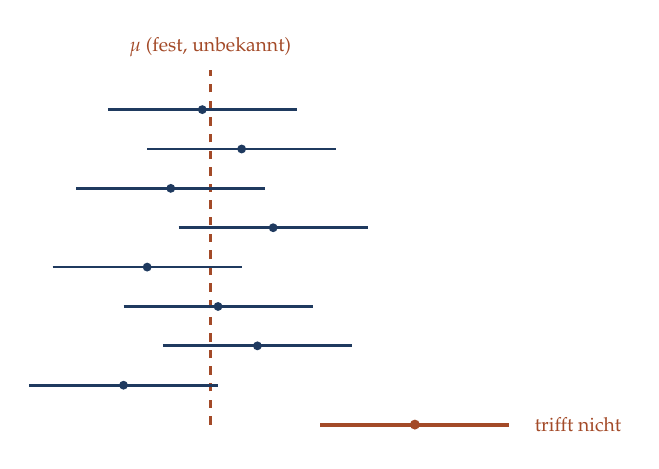
\begin{tikzpicture}[scale=1.0]
\draw[akzent, dashed, line width=1.0pt] (3.2,-0.3) -- (3.2,4.2);
\node[font=\scriptsize, color=akzent] at (3.2,4.5) {$\mu$ (fest, unbekannt)};
\foreach \y/\a/\b in {3.7/1.9/4.3, 3.2/2.4/4.8, 2.7/1.5/3.9, 2.2/2.8/5.2, 1.7/1.2/3.6, 1.2/2.1/4.5, 0.7/2.6/5.0, 0.2/0.9/3.3} {
  \draw[tief, line width=1.0pt] (\a,\y) -- (\b,\y);
  \fill[tief] ({(\a+\b)/2},\y) circle (1.6pt);
}
\draw[akzent, line width=1.4pt] (4.6,-0.3) -- (7.0,-0.3);
\fill[akzent] (5.8,-0.3) circle (1.8pt);
\node[font=\scriptsize, color=akzent, anchor=west] at (7.2,-0.3) {trifft nicht};
\end{tikzpicture}
\end{center}

\begin{center}
\begin{minipage}{0.88\textwidth}
\kursiv{Jede Studie liefert ein anderes Intervall. Die senkrechte Linie steht fest. Die Aussage \enquote{$95\,\%$} betrifft, wie oft die zufälligen Balken die feste Linie treffen --- nicht, wo die Linie liegt.}
\end{minipage}
\end{center}
\end{warnung}

\begin{definition}
\boxtitelm{Definition 6.1 --- Konfidenzintervall}
Ein \Begriff{Konfidenzintervall zum Niveau $1-\alpha$} für einen Parameter $\theta$ ist ein aus den Daten berechnetes Intervall $[U, O]$, für das gilt:
\[ \Pr\bigl[\,U \le \theta \le O\,\bigr] = 1-\alpha \]
--- wobei sich die Wahrscheinlichkeit auf die \kursiv{Zufälligkeit der Grenzen} bezieht, bei festem $\theta$.

Die Eigenschaft heißt \Begriff{Überdeckungswahrscheinlichkeit}.
\end{definition}

\section{Die Deutung --- und fünf falsche}

\begin{merksatz}
\boxtitel{Die einzige richtige Deutung}
\begin{center}
\begin{minipage}{0.9\textwidth}
\textbf{Wendet man das Verfahren auf viele Studien an, so enthalten $95\,\%$ der so erzeugten Intervalle den jeweils wahren Wert.}
\end{minipage}
\end{center}

Die Aussage betrifft also das \kursiv{Verfahren}, nicht das einzelne Intervall. Über das vorliegende Intervall
\[ [14{,}4;\ 21{,}6] \]
lässt sich nur sagen: Es enthält $\mu$, oder es enthält $\mu$ nicht. Welches von beidem gilt, weiß niemand --- und eine Wahrscheinlichkeit dafür gibt es im klassischen Rahmen nicht, weil $\mu$ keine Zufallsgröße ist.
\end{merksatz}

\begin{warnung}
\boxtitelr{Fünf Deutungen, die falsch sind}
\begin{center}
{\small
\renewcommand{\arraystretch}{1.55}
\begin{tabular}{@{}P{0.7cm}P{4.0cm}P{3.6cm}@{}}
\toprule
& \textbf{Aussage} & \textbf{Warum falsch}\\
\midrule
$1$ & \enquote{$\mu$ liegt mit $95\,\%$ Wahrscheinlichkeit in $[14{,}4;\,21{,}6]$.} & $\mu$ ist keine Zufallsgröße. Die Aussage ist entweder wahr oder falsch.\\
$2$ & \enquote{$95\,\%$ der Beobachtungen liegen im Intervall.} & Das wäre ein \Begriff{Prognoseintervall} und wäre viel breiter.\\
$3$ & \enquote{Wiederholt man die Studie, fallen $95\,\%$ der neuen Mittelwerte hinein.} & Tatsächlich sind es etwa $83\,\%$ --- das Intervall ist zu eng dafür.\\
$4$ & \enquote{Wir sind zu $95\,\%$ sicher, dass $\mu$ dort liegt.} & Nur bayessch zulässig, und dann heißt es anders und braucht eine Priori.\\
$5$ & \enquote{Werte außerhalb sind ausgeschlossen.} & Das Intervall trennt nicht in möglich und unmöglich.\\
\bottomrule
\end{tabular}}
\end{center}

\schritt{Zur dritten Zeile --- die Zahl überrascht}
Warum nicht $95\,\%$? Weil ein neuer Mittelwert \kursiv{zwei} Quellen von Zufall hat: Er streut selbst um $\mu$, und das Intervall streut ebenfalls um $\mu$. Beide Streuungen addieren sich. Ein Intervall, das $95\,\%$ künftiger Mittelwerte fangen soll, müsste um den Faktor $\sqrt 2$ breiter sein.

\begin{center}
\begin{minipage}{0.88\textwidth}
\kursiv{Untersuchungen legen Fachleuten genau diese fünf Sätze vor. Die Mehrheit hält mindestens einen für richtig --- unter Studierenden ebenso wie unter Forschenden und Lehrenden. Das ist der Befund aus dem Vorwort, und er ist gut belegt.}
\end{minipage}
\end{center}

\schritt{Was man stattdessen sagen darf}
\begin{center}
\begin{minipage}{0.88\textwidth}
\enquote{Die Daten sind mit Werten zwischen $14{,}4$ und $21{,}6$ Stunden gut verträglich.} Diese Formulierung --- \Begriff{Kompatibilitätsintervall} --- gewinnt seit einigen Jahren an Boden, weil sie keine falsche Wahrscheinlichkeitsaussage nahelegt.
\end{minipage}
\end{center}
\end{warnung}

\section{Der wirkliche Fall: $\sigma$ ist unbekannt}

In Schritt 3 der Herleitung steht $\sigma$. Diese Zahl kennt man nicht; man hat nur $s$.

\begin{warnung}
\boxtitelr{Man darf nicht einfach $s$ einsetzen}
Ersetzt man $\sigma$ durch $s$, so wird der Nenner selbst zufällig. Der Quotient
\[ T = \frac{\overline X - \mu}{s/\sqrt n} \]
ist dann \kursiv{nicht} mehr standardnormalverteilt --- er streut stärker, weil zwei Größen zufällig sind statt einer.

Bei kleinem $n$ ist der Unterschied erheblich. Wer trotzdem mit $1{,}96$ rechnet, bekommt Intervalle, die zu schmal sind und das Niveau verfehlen.
\end{warnung}

\begin{merksatz}
\boxtitel{Die $t$-Verteilung}
Die Größe $T$ folgt der \Begriff{$t$-Verteilung} mit $n-1$ \Begriff{Freiheitsgraden}. Sie sieht der Normalverteilung ähnlich, hat aber schwerere Ränder.

\begin{center}
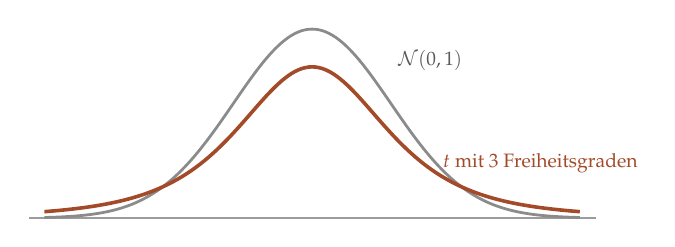
\begin{tikzpicture}[scale=1.0]
\draw[grau!60, line width=0.7pt] (-3.6,0) -- (3.6,0);
\draw[grau!70, line width=1.0pt, smooth, samples=80, domain=-3.4:3.4]
  plot (\x, {2.4*exp(-\x*\x/2)});
\draw[akzent, line width=1.3pt, smooth, samples=80, domain=-3.4:3.4]
  plot (\x, {2.4*0.8*(1+\x*\x/3)^(-2)});
\node[font=\scriptsize, color=grau] at (1.5,2.0) {$\mathcal{N}(0,1)$};
\node[font=\scriptsize, color=akzent] at (2.9,0.7) {$t$ mit $3$ Freiheitsgraden};
\end{tikzpicture}
\end{center}

\schritt{Die Werte, die man braucht}
\begin{center}
{\small
\renewcommand{\arraystretch}{1.38}
\begin{tabular}{@{}P{1.8cm}P{1.8cm}P{1.8cm}P{1.8cm}@{}}
\toprule
\textbf{Freiheits-} & \multicolumn{3}{c}{\textbf{Niveau}}\\
\textbf{grade} & $90\,\%$ & $95\,\%$ & $99\,\%$\\
\midrule
$1$ & $6{,}314$ & $12{,}706$ & $63{,}657$\\
$2$ & $2{,}920$ & $4{,}303$ & $9{,}925$\\
$5$ & $2{,}015$ & $\mathbf{2{,}571}$ & $4{,}032$\\
$10$ & $1{,}812$ & $\mathbf{2{,}228}$ & $3{,}169$\\
$20$ & $1{,}725$ & $2{,}086$ & $2{,}845$\\
$30$ & $1{,}697$ & $2{,}042$ & $2{,}750$\\
$100$ & $1{,}660$ & $1{,}984$ & $2{,}626$\\
$\infty$ & $1{,}645$ & $\mathbf{1{,}960}$ & $2{,}576$\\
\bottomrule
\end{tabular}}
\end{center}

\begin{center}
\begin{minipage}{0.88\textwidth}
\kursiv{Die letzte Zeile ist die Normalverteilung --- bei unendlich vielen Freiheitsgraden fallen beide zusammen. Ab etwa $n = 100$ ist der Unterschied belanglos; bei $n = 6$ beträgt er ein Drittel: $2{,}571$ statt $1{,}960$.}
\end{minipage}
\end{center}
\end{merksatz}

\begin{merksatz}
\boxtitel{Satz 6.2 --- Das $t$-Intervall}
Für normalverteilte Daten ist
\[ \left[\ \MW - t_{n-1;\,1-\alpha/2}\,\frac{s}{\sqrt n}\ ;\ \ \MW + t_{n-1;\,1-\alpha/2}\,\frac{s}{\sqrt n}\ \right] \]
ein Konfidenzintervall zum Niveau $1-\alpha$ für $\mu$.
\end{merksatz}

\begin{merksatz}
\boxtitel{Die MOBIL-Gruppe B, vollständig gerechnet}
\schritt{Schritt 1 --- Die Kennzahlen}
Aus Kapitel~2: $n = 6$, $\MW = 18{,}0$, $s = \sqrt{12} = 3{,}464$.

\schritt{Schritt 2 --- Standardfehler}
\[ \frac{s}{\sqrt n} = \frac{3{,}464}{\sqrt 6} = \frac{3{,}464}{2{,}449} = 1{,}414 . \]

\schritt{Schritt 3 --- Den $t$-Wert nachschlagen}
Freiheitsgrade: $n - 1 = 5$. Niveau $95\,\%$. Tabelle: $t_{5;\,0{,}975} = 2{,}571$.

\schritt{Schritt 4 --- Die halbe Breite}
\[ 2{,}571 \cdot 1{,}414 = 3{,}636 . \]

\schritt{Schritt 5 --- Das Intervall}
\[ 18{,}0 \pm 3{,}636 \quad\Longrightarrow\quad [\,14{,}36\ ;\ 21{,}64\,] \ \text{Stunden} . \]

\schritt{Zum Vergleich: Gruppe A}
$\MW = 26{,}167$, $s = 5{,}913$, $\frac{s}{\sqrt6} = 2{,}414$, halbe Breite $2{,}571 \cdot 2{,}414 = 6{,}206$:
\[ [\,19{,}96\ ;\ 32{,}37\,] \ \text{Stunden} . \]

\schritt{Die Deutung}
\begin{center}
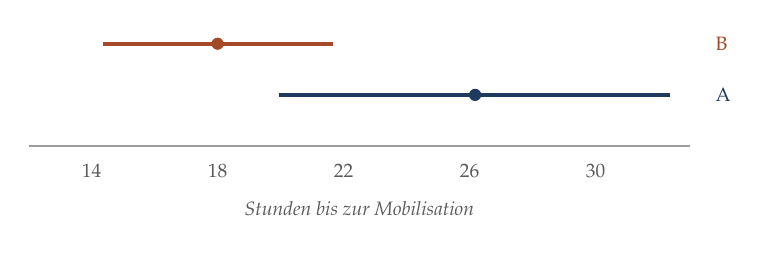
\begin{tikzpicture}[scale=1.0]
\draw[grau!60, line width=0.7pt] (0,0) -- (8.4,0);
\foreach \x/\lab in {0.8/14, 2.4/18, 4.0/22, 5.6/26, 7.2/30}
  \node[font=\scriptsize, color=grau] at (\x,-0.32) {\lab};
\draw[akzent, line width=1.6pt] (0.94,1.3) -- (3.86,1.3);
\fill[akzent] (2.4,1.3) circle (2.2pt);
\node[font=\scriptsize, color=akzent, anchor=west] at (8.6,1.3) {B};
\draw[tief, line width=1.6pt] (3.18,0.65) -- (8.15,0.65);
\fill[tief] (5.67,0.65) circle (2.2pt);
\node[font=\scriptsize, color=tief, anchor=west] at (8.6,0.65) {A};
\node[font=\scriptsize\itshape, color=grau] at (4.2,-0.8) {Stunden bis zur Mobilisation};
\end{tikzpicture}
\end{center}

Die beiden Intervalle überschneiden sich. Das Intervall von A reicht bis $19{,}96$ hinunter, das von B bis $21{,}64$ hinauf.

\begin{center}
\begin{minipage}{0.88\textwidth}
\kursiv{Die naheliegende Folgerung --- \enquote{also kein Unterschied} --- ist voreilig. Der nächste Abschnitt zeigt, warum man für die Frage nach dem \kursiv{Unterschied} ein eigenes Intervall braucht und warum das Überlappen zweier Einzelintervalle kein taugliches Kriterium ist.}
\end{minipage}
\end{center}
\end{merksatz}

\section{Das Intervall für den Unterschied}

\begin{merksatz}
\boxtitel{Warum man es getrennt berechnen muss}
Gefragt ist nicht, wo $\mu_A$ liegt und wo $\mu_B$, sondern wo $\mu_A - \mu_B$ liegt. Das ist ein eigener Parameter und braucht ein eigenes Intervall.

\schritt{Der Standardfehler des Unterschieds}
Nach (R4) --- die Gruppen sind unabhängig --- addieren sich die Varianzen:
\[ \Var[\overline X_A - \overline X_B] = \frac{\sigma^2}{n_A} + \frac{\sigma^2}{n_B} . \]
Nimmt man gleiche Streuung in beiden Gruppen an, so schätzt man $\sigma^2$ aus beiden gemeinsam:
\[ s_p^2 = \frac{(n_A-1)s_A^2 + (n_B-1)s_B^2}{n_A+n_B-2} . \]
Dieser Wert heißt \Begriff{gepoolte Varianz}; er ist das mit den Freiheitsgraden gewichtete Mittel.
\end{merksatz}

\begin{merksatz}
\boxtitel{Die Rechnung für MOBIL}
\schritt{Schritt 1 --- Die gepoolte Varianz}
\[ s_p^2 = \frac{5 \cdot 34{,}967 + 5 \cdot 12{,}0}{6+6-2} = \frac{174{,}83 + 60{,}0}{10} = \frac{234{,}83}{10} = 23{,}483 \]
\[ s_p = \sqrt{23{,}483} = 4{,}846 . \]

\schritt{Schritt 2 --- Der Standardfehler}
\[ \mathrm{SE} = s_p\sqrt{\frac{1}{n_A}+\frac{1}{n_B}} = 4{,}846 \cdot \sqrt{\frac{1}{6}+\frac{1}{6}} = 4{,}846 \cdot \sqrt{0{,}3333} = 4{,}846 \cdot 0{,}5774 = 2{,}798 . \]

\schritt{Schritt 3 --- Der $t$-Wert}
Freiheitsgrade: $n_A + n_B - 2 = 10$. Tabelle: $t_{10;\,0{,}975} = 2{,}228$.

\schritt{Schritt 4 --- Der Unterschied und sein Intervall}
\[ \MW_A - \MW_B = 26{,}167 - 18{,}0 = 8{,}167 \ \text{Stunden} \]
\[ 8{,}167 \pm 2{,}228 \cdot 2{,}798 = 8{,}167 \pm 6{,}234 \]
\[ [\,1{,}93\ ;\ 14{,}40\,] \ \text{Stunden} . \]

\schritt{Die Deutung}
\begin{center}
\begin{minipage}{0.9\textwidth}
Das Intervall \kursiv{enthält die Null nicht}. Die Daten sind also schlecht mit der Annahme verträglich, dass beide Schemata gleich wirken.
\end{minipage}
\end{center}

Und es sagt mehr: Der Unterschied könnte so klein sein wie zwei Stunden oder so groß wie vierzehn. Bei $n=6$ je Gruppe lässt sich nicht genauer eingrenzen.
\end{merksatz}

\begin{warnung}
\boxtitelr{Überlappende Einzelintervalle bedeuten nichts}
Die Einzelintervalle überlappten sich --- das Differenzintervall schließt die Null trotzdem aus. Ein Widerspruch ist das nicht.

\schritt{Der Grund}
Vergleicht man zwei Intervalle der halben Breite $h_A$ und $h_B$, so berührt sich der Rand bei einem Abstand von $h_A + h_B$. Das Differenzintervall hat aber die halbe Breite
\[ t\,s_p\sqrt{\tfrac{1}{n_A}+\tfrac{1}{n_B}} , \]
und wegen $\sqrt{a^2+b^2} < a+b$ ist sie \kursiv{kleiner} als die Summe der beiden Einzelbreiten.

\begin{center}
\renewcommand{\arraystretch}{1.48}
\begin{tabular}{@{}P{3.2cm}P{2.4cm}P{2.4cm}@{}}
\toprule
& \textbf{halbe Breite} & \\
\midrule
Intervall A & $6{,}21$ & \\
Intervall B & $3{,}64$ & \\
Summe & $9{,}85$ & \textcolor{akzent}{zu großzügig}\\
\textbf{Differenzintervall} & $\mathbf{6{,}23}$ & \textcolor{gruen}{richtig}\\
\bottomrule
\end{tabular}
\end{center}

\begin{center}
\begin{minipage}{0.88\textwidth}
\kursiv{Der Beobachtete Abstand beträgt $8{,}17$. Er ist kleiner als $9{,}85$ --- daher überlappen die Einzelintervalle. Und er ist größer als $6{,}23$ --- daher schließt das Differenzintervall die Null aus. Beides gleichzeitig ist der Normalfall, nicht die Ausnahme.}
\end{minipage}
\end{center}

\begin{center}
\begin{minipage}{0.9\textwidth}
\textbf{Merksatz: Wer zwei Gruppen vergleichen will, zeichnet das Intervall für den Unterschied --- nicht zwei Intervalle nebeneinander.}
\end{minipage}
\end{center}
\end{warnung}

\section{Das Intervall für einen Anteil}

\begin{merksatz}
\boxtitel{Die naheliegende Formel --- und ihr Versagen}
Für einen Anteil $\pi$ mit Schätzer $\hat p = k/n$ ist
\[ \Var[\hat p] = \frac{\pi(1-\pi)}{n} , \]
also liegt nahe:
\[ \hat p \pm 1{,}96\,\sqrt{\frac{\hat p(1-\hat p)}{n}} . \]
Das ist das \Begriff{Wald-Intervall}.

\schritt{Am Beispiel}
Gruppe A: $3$ von $6$ brauchten zusätzliche Schmerzmittel, also $\hat p = 0{,}5$.
\[ \sqrt{\frac{0{,}5 \cdot 0{,}5}{6}} = \sqrt{0{,}04167} = 0{,}2041 \]
\[ 0{,}5 \pm 1{,}96 \cdot 0{,}2041 = 0{,}5 \pm 0{,}400 \quad\Longrightarrow\quad [\,0{,}100\ ;\ 0{,}900\,] . \]
\end{merksatz}

\begin{warnung}
\boxtitelr{Das Wald-Intervall bricht zusammen}
\schritt{Fall 1 --- alle oder keiner}
Hätten alle sechs Personen Bedarf gehabt, so wäre $\hat p = 1$ und
\[ \sqrt{\frac{1 \cdot 0}{6}} = 0 \quad\Longrightarrow\quad [\,1{,}000\ ;\ 1{,}000\,] . \]
Das Intervall hat die Breite null. Es behauptet, der Anteil sei mit Gewissheit hundert Prozent --- aus sechs Beobachtungen.

\schritt{Fall 2 --- Grenzen außerhalb des Möglichen}
Bei $\hat p = 0{,}1$ und $n = 20$:
\[ 0{,}1 \pm 1{,}96\sqrt{\frac{0{,}1 \cdot 0{,}9}{20}} = 0{,}1 \pm 1{,}96 \cdot 0{,}0671 = 0{,}1 \pm 0{,}131 \]
\[ [\,-0{,}031\ ;\ 0{,}231\,] . \]
Eine negative untere Grenze für einen Anteil.

\schritt{Fall 3 --- das Niveau stimmt nicht}
Selbst bei mittleren Anteilen liegt die tatsächliche Überdeckung oft bei $88$ bis $92\,\%$ statt bei $95\,\%$ --- und zwar auch bei großem $n$. Die Abweichung verschwindet nicht, sie schwankt nur.

\begin{center}
\begin{minipage}{0.88\textwidth}
\kursiv{Das Wald-Intervall steht in fast jedem Einführungsbuch und ist in Statistikprogrammen oft die Voreinstellung. Es ist dennoch die schlechteste der gebräuchlichen Methoden.}
\end{minipage}
\end{center}
\end{warnung}

\begin{merksatz}
\boxtitel{Das Wilson-Intervall}
\Person{Edwin Wilson} gab 1927 eine bessere Formel an. Sie entsteht, wenn man die Ungleichung nicht nach der Näherung, sondern \kursiv{exakt} nach $\pi$ auflöst:
\[ \frac{\hat p + \frac{z^2}{2n} \;\pm\; \frac{z}{\sqrt n}\sqrt{\hat p(1-\hat p) + \frac{z^2}{4n}}}{1 + \frac{z^2}{n}} \]
mit $z = 1{,}96$.

\schritt{Gruppe A, $k=3$, $n=6$}
Wir rechnen mit $z^2 = 3{,}8416$.
\[ \text{Mitte} = \frac{3 + 1{,}9208}{6 + 3{,}8416} = \frac{4{,}9208}{9{,}8416} = 0{,}5000 \]
\[ \text{halbe Breite} = \frac{1{,}96}{9{,}8416}\sqrt{6 \cdot 0{,}25 + 0{,}9604} = 0{,}1992 \cdot \sqrt{2{,}4604} = 0{,}1992 \cdot 1{,}5686 = 0{,}3124 \]
\[ [\,0{,}188\ ;\ 0{,}812\,] . \]

\schritt{Der Fall $k = 6$, $n = 6$}
\[ \text{Mitte} = \frac{6 + 1{,}9208}{9{,}8416} = \frac{7{,}9208}{9{,}8416} = 0{,}8048 \]
\[ \text{halbe Breite} = 0{,}1992 \cdot \sqrt{0 + 0{,}9604} = 0{,}1992 \cdot 0{,}980 = 0{,}1952 \]
\[ [\,0{,}610\ ;\ 1{,}000\,] . \]

\schritt{Der Vergleich}
\begin{center}
\renewcommand{\arraystretch}{1.48}
\begin{tabular}{@{}P{2.2cm}P{2.8cm}P{2.8cm}@{}}
\toprule
$k/n$ & \textbf{Wald} & \textbf{Wilson}\\
\midrule
$3/6$ & $[0{,}100;\,0{,}900]$ & $[0{,}188;\,0{,}812]$\\
$6/6$ & \textcolor{akzent}{$[1{,}000;\,1{,}000]$} & \textcolor{gruen}{$[0{,}610;\,1{,}000]$}\\
\bottomrule
\end{tabular}
\end{center}

\begin{center}
\begin{minipage}{0.88\textwidth}
\kursiv{Das Wilson-Intervall bleibt stets innerhalb von $[0,1]$, wird nie zum Punkt und hält das Niveau auch bei kleinen $n$ gut ein. Es ist seit fast hundert Jahren bekannt und setzt sich nur langsam durch.}
\end{minipage}
\end{center}
\end{merksatz}

\begin{merksatz}
\boxtitel{Die Dreierregel}
Ein Sonderfall, den man im Kopf haben sollte: Trat ein Ereignis in $n$ Beobachtungen \kursiv{kein einziges Mal} auf, so ist die obere $95$-Prozent-Grenze näherungsweise
\[ \frac{3}{n} . \]

\schritt{Ein Beispiel}
In einer Studie mit $300$ Personen trat keine schwere Nebenwirkung auf. Was heißt das?
\[ \frac{3}{300} = 0{,}01 . \]
Die Daten sind mit einer Rate von bis zu einem Prozent verträglich --- also mit bis zu einer schweren Nebenwirkung je hundert Behandelten.

\begin{center}
\begin{minipage}{0.88\textwidth}
\kursiv{\enquote{Keine Nebenwirkung beobachtet} heißt nicht \enquote{keine Nebenwirkung vorhanden}. Bei $n = 300$ sind Raten bis $1\,\%$ gut verträglich mit dem Befund. Wer für eine seltene Nebenwirkung von $1$ zu $10\,000$ Sicherheit will, braucht etwa $30\,000$ Beobachtungen.}
\end{minipage}
\end{center}
\end{merksatz}

\section{Übungsaufgaben}

\begin{aufgabe}
\boxtitel{Aufgabe 6.1 --- Ein Intervall und seine Deutung}
Eine Studie mit $n=25$ berichtet $\MW = 42{,}0$ und $s = 10{,}0$.
\begin{center}
{\small
\renewcommand{\arraystretch}{1.35}
\begin{tabular}{@{}P{4.2cm}P{4.2cm}@{}}
\toprule
(a) $95$-Prozent-Intervall & (c) Welches $n$ für halbe Breite $2$?\\
(b) $99$-Prozent-Intervall & (d) Welche Deutungen sind zulässig?\\
\bottomrule
\end{tabular}}
\end{center}

\loesung
\schritt{(a) --- Das $95$-Prozent-Intervall}
\[ \frac{s}{\sqrt n} = \frac{10}{\sqrt{25}} = \frac{10}{5} = 2{,}0 \]
Freiheitsgrade $24$; die Tabelle gibt zwischen $20$ und $30$ etwa $t_{24;\,0{,}975} \approx 2{,}064$.
\[ 42{,}0 \pm 2{,}064 \cdot 2{,}0 = 42{,}0 \pm 4{,}13 \quad\Longrightarrow\quad [\,37{,}87\ ;\ 46{,}13\,] . \]

\schritt{(b) --- Das $99$-Prozent-Intervall}
$t_{24;\,0{,}995} \approx 2{,}797$.
\[ 42{,}0 \pm 2{,}797 \cdot 2{,}0 = 42{,}0 \pm 5{,}59 \quad\Longrightarrow\quad [\,36{,}41\ ;\ 47{,}59\,] . \]

\schritt{Die Beobachtung}
Mehr Sicherheit bedeutet ein breiteres Intervall. Man kann nicht beides zugleich haben.
\begin{center}
\renewcommand{\arraystretch}{1.42}
\begin{tabular}{@{}P{2.2cm}P{2.2cm}P{2.6cm}@{}}
\toprule
\textbf{Niveau} & \textbf{halbe Breite} & \\
\midrule
$90\,\%$ & $3{,}42$ & \\
$95\,\%$ & $4{,}13$ & \\
$99\,\%$ & $5{,}59$ & \\
$100\,\%$ & $\infty$ & \textcolor{akzent}{nutzlos}\\
\bottomrule
\end{tabular}
\end{center}
Die letzte Zeile zeigt die Grenze des Verfahrens: Völlige Sicherheit gibt es nur um den Preis einer Aussage ohne Inhalt.

\schritt{(c) --- Die nötige Fallzahl}
\[ 2{,}0 \ \ge\ t \cdot \frac{10}{\sqrt n} \]
Wir rechnen zunächst mit $t \approx 2{,}0$ und prüfen danach:
\[ \sqrt n \ge \frac{2{,}0 \cdot 10}{2{,}0} = 10 \quad\Longrightarrow\quad n \ge 100 . \]
Kontrolle: Bei $n = 100$ ist $t_{99;\,0{,}975} \approx 1{,}984$, also
\[ 1{,}984 \cdot \frac{10}{10} = 1{,}98 \le 2{,}0 . \quad \checkmark \]

\schritt{Antwort}
Etwa $\mathbf{100}$ Beobachtungen --- das Vierfache für die halbe Breite, wie die Wurzelregel es verlangt.

\schritt{(d) --- Die Deutungen}
\begin{center}
{\small
\renewcommand{\arraystretch}{1.45}
\begin{tabular}{@{}P{4.4cm}P{3.4cm}@{}}
\toprule
\enquote{$\mu$ liegt zu $95\,\%$ drin} & \textcolor{akzent}{unzulässig}\\
\enquote{$95\,\%$ der Werte liegen drin} & \textcolor{akzent}{unzulässig}\\
\enquote{Das Verfahren trifft in $95\,\%$ der Anwendungen} & \textcolor{gruen}{zulässig}\\
\enquote{Die Daten sind mit Werten von $37{,}9$ bis $46{,}1$ gut verträglich} & \textcolor{gruen}{zulässig}\\
\enquote{Der Wert $50$ ist ausgeschlossen} & \textcolor{akzent}{unzulässig}\\
\bottomrule
\end{tabular}}
\end{center}
\end{aufgabe}

\begin{aufgabe}
\boxtitel{Aufgabe 6.2 --- Anteil mit beiden Verfahren}
In einer Nachuntersuchung traten bei $2$ von $40$ Personen Wundheilungsstörungen auf. Berechnen Sie das Wald- und das Wilson-Intervall und vergleichen Sie.

\loesung
\schritt{Schritt 1 --- Der Punktschätzer}
\[ \hat p = \frac{2}{40} = 0{,}05 . \]

\schritt{Schritt 2 --- Wald}
\[ \sqrt{\frac{0{,}05 \cdot 0{,}95}{40}} = \sqrt{\frac{0{,}0475}{40}} = \sqrt{0{,}0011875} = 0{,}03446 \]
\[ 0{,}05 \pm 1{,}96 \cdot 0{,}03446 = 0{,}05 \pm 0{,}0675 \quad\Longrightarrow\quad [\,-0{,}018\ ;\ 0{,}118\,] . \]
Die untere Grenze ist negativ --- unmöglich für einen Anteil.

\schritt{Schritt 3 --- Wilson}
Mit $z^2 = 3{,}8416$ und $n = 40$:
\[ \text{Nenner} = 40 + 3{,}8416 = 43{,}8416 \]
\[ \text{Zähler der Mitte} = 2 + 1{,}9208 = 3{,}9208 \quad\Longrightarrow\quad \text{Mitte} = \frac{3{,}9208}{43{,}8416} = 0{,}0894 \]

Für die halbe Breite:
\[ n\hat p(1-\hat p) + \frac{z^2}{4} = 40 \cdot 0{,}0475 + 0{,}9604 = 1{,}90 + 0{,}9604 = 2{,}8604 \]
\[ \sqrt{2{,}8604} = 1{,}6913 \]
\[ \text{halbe Breite} = \frac{1{,}96}{43{,}8416} \cdot 1{,}6913 = 0{,}04471 \cdot 1{,}6913 = 0{,}0756 \]

\[ [\,0{,}0894 - 0{,}0756\ ;\ 0{,}0894 + 0{,}0756\,] = [\,0{,}014\ ;\ 0{,}165\,] . \]

\schritt{Schritt 4 --- Der Vergleich}
\begin{center}
\renewcommand{\arraystretch}{1.48}
\begin{tabular}{@{}P{2.2cm}P{2.8cm}P{2.8cm}@{}}
\toprule
& \textbf{Wald} & \textbf{Wilson}\\
\midrule
Intervall & $[-0{,}018;\,0{,}118]$ & $[0{,}014;\,0{,}165]$\\
Untere Grenze & \textcolor{akzent}{negativ} & \textcolor{gruen}{$1{,}4\,\%$}\\
Obere Grenze & $11{,}8\,\%$ & $16{,}5\,\%$\\
Lage zum Schätzer & symmetrisch & \textcolor{gruen}{nach oben verschoben}\\
\bottomrule
\end{tabular}
\end{center}

\schritt{Schritt 5 --- Warum Wilson nach oben verschoben ist}
Bei kleinen Anteilen ist die Verteilung von $\hat p$ schief: Nach unten ist bei null Schluss, nach oben ist Platz. Ein symmetrisches Intervall bildet das falsch ab.

Wilson trägt dem Rechnung --- der Mittelpunkt $0{,}089$ liegt über dem Schätzer $0{,}05$. Das sieht ungewohnt aus und ist richtig.

\schritt{Die Deutung}
Die Daten sind mit einer Störungsrate zwischen etwa $1{,}5$ und $16{,}5$ Prozent gut verträglich. Bei $40$ Beobachtungen und zwei Ereignissen lässt sich nicht mehr sagen.

\begin{center}
\begin{minipage}{0.86\textwidth}
\kursiv{Wer aus \enquote{$5\,\%$ Komplikationsrate} eine Planungsgröße macht, ohne das Intervall zu nennen, gibt eine Genauigkeit vor, die die Daten nicht hergeben. Die obere Grenze ist mehr als dreimal so groß wie der Punktschätzer.}
\end{minipage}
\end{center}
\end{aufgabe}

\begin{aufgabe}
\boxtitel{Aufgabe 6.3 --- Das Überlappungsproblem}
Zwei Gruppen mit je $n=25$: $\MW_1 = 50$, $\MW_2 = 44$, beide $s = 10$. Zeigen Sie, dass sich die Einzelintervalle überlappen, das Differenzintervall die Null aber ausschließt.

\loesung
\schritt{Schritt 1 --- Die Einzelintervalle}
$\frac{s}{\sqrt n} = \frac{10}{5} = 2{,}0$, $t_{24;\,0{,}975} = 2{,}064$, halbe Breite $4{,}13$.
\[ \text{Gruppe 1:}\ [\,45{,}87\ ;\ 54{,}13\,], \qquad \text{Gruppe 2:}\ [\,39{,}87\ ;\ 48{,}13\,] . \]

\schritt{Schritt 2 --- Überlappen sie?}
Der Bereich von $45{,}87$ bis $48{,}13$ gehört zu beiden. \textbf{Ja, sie überlappen} --- über eine Spanne von $2{,}26$.

\schritt{Schritt 3 --- Das Differenzintervall}
Gepoolte Varianz bei gleichen $s$ und gleichen $n$:
\[ s_p^2 = \frac{24 \cdot 100 + 24 \cdot 100}{48} = 100, \qquad s_p = 10 . \]
\[ \mathrm{SE} = 10\sqrt{\frac{1}{25}+\frac{1}{25}} = 10\sqrt{0{,}08} = 10 \cdot 0{,}2828 = 2{,}828 \]
Freiheitsgrade $25+25-2 = 48$; $t_{48;\,0{,}975} \approx 2{,}011$.
\[ 6{,}0 \pm 2{,}011 \cdot 2{,}828 = 6{,}0 \pm 5{,}687 \quad\Longrightarrow\quad [\,0{,}31\ ;\ 11{,}69\,] . \]

\schritt{Schritt 4 --- Die Null ist ausgeschlossen}
Die untere Grenze $0{,}31$ liegt über null. \checkmark

\schritt{Schritt 5 --- Die Rechnung, die den scheinbaren Widerspruch auflöst}
\begin{center}
\renewcommand{\arraystretch}{1.48}
\begin{tabular}{@{}P{3.6cm}P{2.2cm}P{2.4cm}@{}}
\toprule
\textbf{Größe} & \textbf{Wert} & \\
\midrule
Beobachteter Abstand & $6{,}00$ & \\
Summe der halben Breiten & $8{,}26$ & \textcolor{akzent}{Überlappung}\\
Halbe Breite der Differenz & $\mathbf{5{,}69}$ & \textcolor{gruen}{Null ausgeschlossen}\\
\bottomrule
\end{tabular}
\end{center}

Der Abstand $6{,}00$ liegt zwischen $5{,}69$ und $8{,}26$ --- genau in dem Bereich, in dem beide Beobachtungen gleichzeitig zutreffen.

\schritt{Schritt 6 --- Wie groß der Bereich ist}
Bei gleichen Gruppen ist die Summe der halben Breiten $2h$ und die halbe Breite der Differenz etwa $h\sqrt 2$. Das Verhältnis beträgt
\[ \frac{2}{\sqrt2} = \sqrt2 \approx 1{,}41 . \]
Für jeden Abstand zwischen $h\sqrt2$ und $2h$ --- also über eine Spanne von etwa $41\,\%$ --- überlappen die Einzelintervalle, obwohl der Unterschied nachweisbar ist.

\begin{center}
\begin{minipage}{0.86\textwidth}
\kursiv{Das ist kein Randfall. Gut ein Drittel aller nachweisbaren Unterschiede fällt in diesen Bereich. Wer Ergebnisse als zwei Balken mit Fehlerintervallen darstellt und die Überlappung prüft, übersieht systematisch echte Unterschiede.}
\end{minipage}
\end{center}
\end{aufgabe}

\begin{geschichte}
\boxtitelg{Ein Brauereichemiker und ein polnischer Mathematiker}
\Person{William Sealy Gosset} (1876--1937) arbeitete ab 1899 bei der Brauerei Guinness in Dublin. Seine Aufgabe war die Qualitätskontrolle --- Gerste, Hopfen, Hefe --- mit kleinen Stichproben, weil jede Messung teuer war.

Die vorhandene Statistik half ihm nicht: Sie war für große Stichproben gebaut. Gosset leitete 1908 die Verteilung des Quotienten $\frac{\overline X - \mu}{s/\sqrt n}$ her --- für den Fall, dass $\sigma$ geschätzt werden muss.

Guinness untersagte den Angestellten Veröffentlichungen, weil ein früherer Mitarbeiter Betriebsgeheimnisse preisgegeben hatte. Gosset veröffentlichte daher unter dem Decknamen \kursiv{Student}. Die Verteilung heißt bis heute so.

\begin{center}
\begin{minipage}{0.9\textwidth}
\kursiv{Der Fall ist ungewöhnlich: Ein zentrales Werkzeug der Wissenschaft entstand in einer Brauerei, aus einem betriebswirtschaftlichen Bedürfnis, und erschien anonym. Gossets Vorgesetzte erfuhren erst nach seinem Tod vom Umfang seiner Arbeiten.}
\end{minipage}
\end{center}

Das Konfidenzintervall selbst ist jünger. \Person{Jerzy Neyman} führte es 1937 ein und legte dabei die Deutung fest, die dieses Kapitel vorträgt --- ausdrücklich als Aussage über das Verfahren, nicht über den Einzelfall. Er schrieb, die Wahrscheinlichkeit beziehe sich auf das \kursiv{langfristige Verhalten} der Methode.

\begin{center}
\begin{minipage}{0.9\textwidth}
\kursiv{Neyman war sich der Missverständlichkeit bewusst und warnte davor. Neunzig Jahre später ist die Warnung unverändert nötig.}
\end{minipage}
\end{center}
\end{geschichte}

\begin{forschung}
\boxtitelp{Vom Test zur Schätzung}
Seit etwa 2015 verschiebt sich die Berichtspraxis in der medizinischen Forschung spürbar.

\begin{center}
{\small
\renewcommand{\arraystretch}{1.45}
\begin{tabular}{@{}P{2.6cm}P{5.6cm}@{}}
\toprule
\textbf{Früher} & \enquote{Der Unterschied war signifikant ($p < 0{,}05$).}\\
\textbf{Heute gefordert} & \enquote{Der Unterschied betrug $8{,}2$ Stunden ($95\,\%$-KI $1{,}9$ bis $14{,}4$).}\\
\bottomrule
\end{tabular}}
\end{center}

Die Gründe:

\begin{center}
\renewcommand{\arraystretch}{1.5}
\begin{tabular}{@{}P{2.6cm}P{6.0cm}@{}}
\toprule
\textbf{Größe sichtbar} & Das Intervall nennt den Effekt in der Einheit der Sache, nicht in einer Wahrscheinlichkeit.\\
\textbf{Genauigkeit sichtbar} & Ein breites Intervall verrät eine kleine Studie; ein $p$-Wert tut das nicht.\\
\textbf{Metaanalyse} & Kapitel~14 braucht Schätzwerte und Standardfehler --- ein $p$-Wert allein genügt nicht.\\
\bottomrule
\end{tabular}
\end{center}

Die CONSORT-Empfehlungen verlangen Effektschätzer mit Intervall für jeden primären und sekundären Endpunkt. Mehrere Zeitschriften --- darunter \kursiv{Epidemiology} seit den 1990er Jahren --- haben $p$-Werte weitgehend verbannt.

\begin{center}
\begin{minipage}{0.88\textwidth}
\kursiv{Die Bewegung geht weiter: Ein Vorschlag von Amrhein, Greenland und McShane (2019), unterzeichnet von über achthundert Fachleuten, fordert, das Wort \enquote{signifikant} ganz aufzugeben und statt dessen Kompatibilitätsintervalle zu berichten. Kapitel~15 stellt die Debatte vollständig dar.}
\end{minipage}
\end{center}
\end{forschung}

\begin{merksatz}
\boxtitel{Was Sie jetzt können}
\begin{center}
\renewcommand{\arraystretch}{1.5}
\begin{tabular}{@{}P{3.2cm}P{5.4cm}@{}}
\toprule
\textbf{Definition 6.1} & Konfidenzintervall über die Überdeckung des \kursiv{Verfahrens}\\
\textbf{Fünf Fehldeutungen} & und warum jede einzelne falsch ist\\
\textbf{Satz 6.2} & Das $t$-Intervall bei unbekanntem $\sigma$\\
\textbf{Differenz\-intervall} & und warum Überlappung nichts bedeutet\\
\textbf{Wilson} & statt Wald bei Anteilen; die Dreierregel\\
\bottomrule
\end{tabular}
\end{center}

\begin{center}
\begin{minipage}{0.88\textwidth}
\kursiv{Damit endet Teil~II. Im nächsten Kapitel kommt die zweite Fehldeutung aus dem Vorwort an die Reihe --- und sie ist die folgenreichere.}
\end{minipage}
\end{center}
\end{merksatz}

\part{Testen}

\chapter{Die Logik des Tests}

\section{Die Frage}

Gruppe B mobilisierte im Mittel $8{,}2$ Stunden früher als Gruppe A. Das ist ein Unterschied in den Daten. Die Frage lautet: Ist er mehr als Zufall?

\begin{merksatz}
\boxtitel{Warum die Frage überhaupt nötig ist}
Auch wenn beide Schemata völlig gleich wirkten, wären die beiden Gruppenmittelwerte nicht exakt gleich --- verschiedene Menschen, verschiedene Werte. Ein Unterschied von null wäre sogar erstaunlich.

\begin{center}
\begin{minipage}{0.9\textwidth}
Die Frage ist also nicht, \kursiv{ob} ein Unterschied vorliegt --- das tut er immer ---, sondern ob er größer ist, als man bei reinem Zufall erwarten würde.
\end{minipage}
\end{center}
\end{merksatz}

\section{Die beiden Hypothesen}

\begin{definition}
\boxtitelm{Definition 7.1}
\begin{itemize}[leftmargin=1.4em, itemsep=4pt]
\item Die \Begriff{Nullhypothese} $H_0$ ist die Annahme, dass kein Effekt vorliegt --- im Beispiel $\mu_A = \mu_B$.
\item Die \Begriff{Alternativhypothese} $H_1$ ist die Gegenannahme --- im Beispiel $\mu_A \neq \mu_B$.
\end{itemize}
\end{definition}

\begin{merksatz}
\boxtitel{Warum die Nullhypothese die langweilige ist}
Die Aufteilung ist nicht symmetrisch. $H_0$ ist stets diejenige Hypothese, die einen \kursiv{genauen Wert} festlegt.

\begin{center}
\renewcommand{\arraystretch}{1.55}
\begin{tabular}{@{}P{2.0cm}P{2.4cm}P{4.0cm}@{}}
\toprule
& \textbf{Aussage} & \textbf{Rechenbar?}\\
\midrule
$H_0$ & $\mu_A - \mu_B = 0$ & \textcolor{gruen}{ja --- ein Wert}\\
$H_1$ & $\mu_A - \mu_B \neq 0$ & \textcolor{akzent}{nein --- unendlich viele}\\
\bottomrule
\end{tabular}
\end{center}

\begin{center}
\begin{minipage}{0.88\textwidth}
\kursiv{Man kann ausrechnen, wie wahrscheinlich die Daten unter \kursiv{einem} festen Wert sind. Unter \enquote{irgendein Unterschied} kann man nichts ausrechnen --- wäre der wahre Unterschied $0{,}1$ Stunden oder $50$? Deshalb wird stets gegen $H_0$ gerechnet und nie für $H_1$.}
\end{minipage}
\end{center}
\end{merksatz}

\begin{merksatz}
\boxtitel{Die Beweisfigur}
Der Test ist ein Widerspruchsbeweis mit einer Abschwächung.

\begin{center}
\renewcommand{\arraystretch}{1.55}
\begin{tabular}{@{}P{2.4cm}P{6.2cm}@{}}
\toprule
\textbf{In der Mathematik} & Annahme $\Rightarrow$ Widerspruch $\Rightarrow$ Annahme falsch.\\
\textbf{Im Test} & Annahme $\Rightarrow$ die Daten wären sehr unwahrscheinlich $\Rightarrow$ \kursiv{Zweifel} an der Annahme.\\
\bottomrule
\end{tabular}
\end{center}

\begin{center}
\begin{minipage}{0.88\textwidth}
\kursiv{Der Unterschied ist wesentlich. Ein Widerspruch ist endgültig; ein unwahrscheinliches Ereignis ist möglich. Deshalb kann ein Test nie beweisen --- weder $H_0$ noch $H_1$.}
\end{minipage}
\end{center}
\end{merksatz}

\section{Der $p$-Wert}

\begin{definition}
\boxtitelm{Definition 7.2 --- der $p$-Wert}
Der \Begriff{$p$-Wert} ist die Wahrscheinlichkeit, \kursiv{unter der Annahme, dass $H_0$ zutrifft}, einen Wert der Teststatistik zu erhalten, der mindestens so weit von der Nullhypothese entfernt liegt wie der tatsächlich beobachtete.
\end{definition}

\begin{merksatz}
\boxtitel{Die Definition Stück für Stück}
\begin{center}
{\small
\renewcommand{\arraystretch}{1.55}
\begin{tabular}{@{}P{3.4cm}P{5.0cm}@{}}
\toprule
\textbf{Wahrscheinlichkeit} & Nicht der Daten schlechthin, sondern einer \kursiv{Menge} von möglichen Ergebnissen.\\
\textbf{unter $H_0$} & Es wird gerechnet, \kursiv{als ob} $H_0$ zuträfe. Ob sie zutrifft, bleibt offen.\\
\textbf{mindestens so weit entfernt} & Nicht nur das beobachtete Ergebnis, sondern auch alle noch extremeren.\\
\bottomrule
\end{tabular}}
\end{center}

\begin{center}
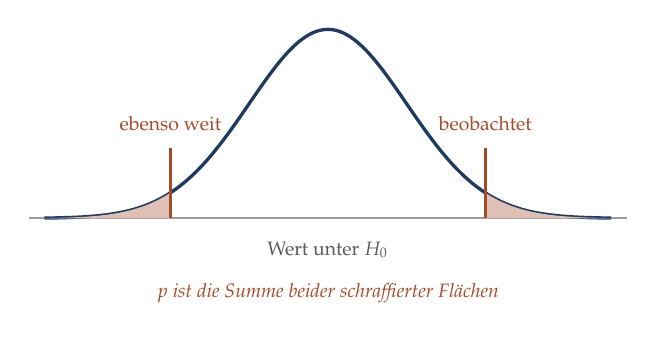
\begin{tikzpicture}[scale=1.0]
\draw[grau!60, line width=0.7pt] (-3.8,0) -- (3.8,0);
\draw[tief, line width=1.2pt, smooth, samples=90, domain=-3.6:3.6]
  plot (\x, {2.4*exp(-\x*\x/2)});
\fill[akzent!35] plot[smooth, samples=30, domain=2.0:3.6] (\x,{2.4*exp(-\x*\x/2)}) -- (3.6,0) -- (2.0,0) -- cycle;
\fill[akzent!35] plot[smooth, samples=30, domain=-3.6:-2.0] (\x,{2.4*exp(-\x*\x/2)}) -- (-2.0,0) -- (-3.6,0) -- cycle;
\draw[akzent, line width=1.0pt] (2.0,0) -- (2.0,0.9);
\draw[akzent, line width=1.0pt] (-2.0,0) -- (-2.0,0.9);
\node[font=\scriptsize, color=akzent] at (2.0,1.2) {beobachtet};
\node[font=\scriptsize, color=akzent] at (-2.0,1.2) {ebenso weit};
\node[font=\scriptsize, color=grau] at (0,-0.4) {Wert unter $H_0$};
\node[font=\scriptsize\itshape, color=akzent] at (0,-0.95) {$p$ ist die Summe beider schraffierter Flächen};
\end{tikzpicture}
\end{center}

\schritt{Warum auch die extremeren Werte zählen}
Bei einer stetigen Größe ist die Wahrscheinlichkeit jedes \kursiv{einzelnen} Werts null. Die Frage \enquote{wie wahrscheinlich war genau dieses Ergebnis?} hat also die Antwort null und ist unbrauchbar.

Sinnvoll fragen lässt sich nur: Wie wahrscheinlich wäre ein Ergebnis, das mindestens so auffällig ist? Das ist eine Fläche, keine Einzelwahrscheinlichkeit.

\schritt{Warum auf beiden Seiten}
Fragt man nach \kursiv{irgendeinem} Unterschied --- ohne Richtungsvorgabe ---, so ist eine Abweichung nach unten ebenso auffällig wie eine nach oben. Beide Flächen zählen. Man spricht vom \Begriff{zweiseitigen} Test.
\end{merksatz}

\begin{warnung}
\boxtitelr{Sieben Deutungen, die falsch sind}
\begin{center}
{\small
\renewcommand{\arraystretch}{1.5}
\begin{tabular}{@{}P{0.7cm}P{3.8cm}P{3.8cm}@{}}
\toprule
& \textbf{Aussage} & \textbf{Warum falsch}\\
\midrule
$1$ & \enquote{$p$ ist die Wahrscheinlichkeit, dass $H_0$ stimmt.} & $H_0$ ist keine Zufallsgröße. $p$ wird \kursiv{unter} $H_0$ gerechnet, nicht \kursiv{über} sie.\\
$2$ & \enquote{$1-p$ ist die Wahrscheinlichkeit, dass $H_1$ stimmt.} & Folgt aus dem ersten Fehler.\\
$3$ & \enquote{$p$ ist die Wahrscheinlichkeit, dass das Ergebnis auf Zufall beruht.} & Dieselbe Verwechslung, anders formuliert.\\
$4$ & \enquote{Ein kleines $p$ bedeutet einen großen Effekt.} & $p$ hängt auch von $n$ ab. Abschnitt 7.6.\\
$5$ & \enquote{$p > 0{,}05$ heißt, es gibt keinen Unterschied.} & Heißt nur: kein Nachweis. Abschnitt 7.5.\\
$6$ & \enquote{$p$ ist die Fehlerwahrscheinlichkeit dieser Entscheidung.} & Das wäre $\alpha$, und das wird \kursiv{vorher} festgelegt.\\
$7$ & \enquote{Bei Wiederholung wird das Ergebnis mit Wahrscheinlichkeit $1-p$ wieder signifikant.} & Bei $p = 0{,}05$ liegt die Chance tatsächlich bei etwa $50\,\%$.\\
\bottomrule
\end{tabular}}
\end{center}

\schritt{Der Kern aller sieben}
Sie alle verwechseln
\[ \Pr[\text{Daten} \mid H_0] \qquad \text{mit} \qquad \Pr[H_0 \mid \text{Daten}] . \]

\begin{center}
\begin{minipage}{0.88\textwidth}
\kursiv{Dass diese beiden Größen verschieden sind, ist aus der Medizin vertraut: Die Wahrscheinlichkeit eines positiven Tests bei Krankheit --- die Sensitivität --- ist etwas anderes als die Wahrscheinlichkeit einer Krankheit bei positivem Test. Kapitel~13 rechnet den Unterschied vor. Es ist derselbe Fehler.}
\end{minipage}
\end{center}

\schritt{Zur siebten Zeile}
Die Zahl überrascht und ist nachrechenbar: Ist der beobachtete Effekt zufällig gerade so groß, dass $p = 0{,}05$ herauskommt, so liegt der wahre Effekt vermutlich in dieser Größenordnung --- und dann trifft die Wiederholung mit etwa gleicher Wahrscheinlichkeit darüber wie darunter. Die Macht einer Wiederholung liegt bei rund $50\,\%$.
\end{warnung}

\begin{merksatz}
\boxtitel{Was der $p$-Wert wirklich ist}
\begin{center}
\begin{minipage}{0.9\textwidth}
\textbf{Ein Maß für die Verträglichkeit der Daten mit der Nullhypothese.} Klein heißt: Unter $H_0$ wären solche Daten selten. Mehr sagt er nicht --- insbesondere nichts über die Größe des Effekts und nichts über die Wahrscheinlichkeit irgendeiner Hypothese.
\end{minipage}
\end{center}
\end{merksatz}

\section{Die beiden Fehler}

\begin{definition}
\boxtitelm{Definition 7.3}
\begin{center}
{\small
\renewcommand{\arraystretch}{1.6}
\begin{tabular}{@{}P{2.4cm}P{2.8cm}P{2.8cm}@{}}
\toprule
& \textbf{$H_0$ trifft zu} & \textbf{$H_1$ trifft zu}\\
\midrule
$H_0$ beibehalten & \textcolor{gruen}{richtig} & \textcolor{akzent}{\textbf{Fehler 2. Art}} ($\beta$)\\
$H_0$ verwerfen & \textcolor{akzent}{\textbf{Fehler 1. Art}} ($\alpha$) & \textcolor{gruen}{richtig} (Macht $1-\beta$)\\
\bottomrule
\end{tabular}}
\end{center}
\end{definition}

\begin{merksatz}
\boxtitel{Die beiden Fehler in der Sprache der Diagnostik}
\begin{center}
\renewcommand{\arraystretch}{1.5}
\begin{tabular}{@{}P{2.6cm}P{6.0cm}@{}}
\toprule
\textbf{Fehler 1. Art} & Ein Effekt wird behauptet, den es nicht gibt --- \kursiv{falsch positiv}.\\
\textbf{Fehler 2. Art} & Ein vorhandener Effekt wird übersehen --- \kursiv{falsch negativ}.\\
\textbf{Macht} & Die Wahrscheinlichkeit, einen vorhandenen Effekt zu finden --- die \kursiv{Sensitivität} des Tests.\\
\bottomrule
\end{tabular}
\end{center}

\schritt{Die übliche Wahl}
\begin{center}
\renewcommand{\arraystretch}{1.45}
\begin{tabular}{@{}P{1.6cm}P{2.0cm}P{4.4cm}@{}}
\toprule
$\alpha$ & $0{,}05$ & Konvention, keine Herleitung\\
$\beta$ & $0{,}20$ & entspricht $80\,\%$ Macht\\
\bottomrule
\end{tabular}
\end{center}

\begin{center}
\begin{minipage}{0.88\textwidth}
\kursiv{Beachten Sie die Asymmetrie: Der Fehler erster Art wird viermal strenger begrenzt als der zweiter Art. Das ist eine Wertentscheidung --- man hält es für schlimmer, einen Effekt zu behaupten, den es nicht gibt, als einen zu übersehen. Ob das in jedem Fall richtig ist, ist eine sachliche Frage. Bei der Prüfung einer Nebenwirkung wäre eher das Umgekehrte angebracht.}
\end{minipage}
\end{center}
\end{merksatz}

\begin{warnung}
\boxtitelr{$\alpha$ und $p$ sind verschiedene Dinge}
\begin{center}
\renewcommand{\arraystretch}{1.55}
\begin{tabular}{@{}P{1.6cm}P{6.8cm}@{}}
\toprule
$\alpha$ & Wird \kursiv{vor} der Studie festgelegt. Eine Eigenschaft des \kursiv{Verfahrens}: Wie oft darf es fälschlich Alarm schlagen?\\
$p$ & Wird \kursiv{aus} den Daten berechnet. Eine Eigenschaft dieser \kursiv{einen} Studie.\\
\bottomrule
\end{tabular}
\end{center}

Die Entscheidungsregel lautet: Verwirf $H_0$, falls $p \le \alpha$. Dadurch wird die Rate falscher Alarme über viele Studien hinweg auf $\alpha$ begrenzt.

\begin{center}
\begin{minipage}{0.88\textwidth}
\kursiv{Es ist dieselbe Denkfigur wie beim Konfidenzintervall: Die Garantie betrifft das Verfahren über viele Anwendungen, nicht die einzelne Entscheidung. Deshalb ist die sechste Fehldeutung oben falsch.}
\end{minipage}
\end{center}
\end{warnung}

\section{Der Ablauf --- und die MOBIL-Daten}

\begin{merksatz}
\boxtitel{Sieben Schritte}
\begin{center}
\renewcommand{\arraystretch}{1.5}
\begin{tabular}{@{}P{1.0cm}P{7.4cm}@{}}
\toprule
$1$ & Hypothesen festlegen --- \kursiv{vor} dem Blick auf die Daten.\\
$2$ & Niveau $\alpha$ festlegen --- ebenfalls vorher.\\
$3$ & Verfahren wählen und seine Voraussetzungen prüfen.\\
$4$ & Teststatistik berechnen.\\
$5$ & $p$-Wert bestimmen.\\
$6$ & Entscheiden.\\
$7$ & \textbf{Effektschätzer mit Konfidenzintervall angeben.}\\
\bottomrule
\end{tabular}
\end{center}

\begin{center}
\begin{minipage}{0.88\textwidth}
\kursiv{Schritt 7 fehlt in vielen Darstellungen und ist der wichtigste. Ein Test allein sagt nur \enquote{ja} oder \enquote{nein}; das Intervall sagt, worum es geht.}
\end{minipage}
\end{center}
\end{merksatz}

\begin{merksatz}
\boxtitel{Der $t$-Test für MOBIL, vollständig}
\schritt{Schritt 1 --- Hypothesen}
\[ H_0: \mu_A = \mu_B \qquad \text{gegen} \qquad H_1: \mu_A \neq \mu_B \]

\schritt{Schritt 2 --- Niveau}
$\alpha = 0{,}05$, zweiseitig.

\schritt{Schritt 3 --- Voraussetzungen}
\begin{center}
\renewcommand{\arraystretch}{1.45}
\begin{tabular}{@{}P{3.0cm}P{1.8cm}P{3.4cm}@{}}
\toprule
\textbf{Voraussetzung} & \textbf{Erfüllt?} & \\
\midrule
Unabhängigkeit & \textcolor{gruen}{ja} & verschiedene Personen\\
Normal\-verteilung & \textcolor{mittel}{ungeprüft} & bei $n=6$ kaum prüfbar\\
Gleiche Varianzen & \textcolor{mittel}{fraglich} & $34{,}97$ gegen $12{,}0$\\
\bottomrule
\end{tabular}
\end{center}

\begin{center}
\begin{minipage}{0.86\textwidth}
\kursiv{Zwei der drei Voraussetzungen sind unsicher. Wir rechnen trotzdem weiter --- und kommen in Kapitel~8 und 9 darauf zurück, was das bedeutet und was man stattdessen tun kann.}
\end{minipage}
\end{center}

\schritt{Schritt 4 --- Die Teststatistik}
Aus Kapitel~6: $\MW_A - \MW_B = 8{,}167$ und $\mathrm{SE} = 2{,}798$.
\[ t = \frac{8{,}167}{2{,}798} = 2{,}919 \]
bei $n_A + n_B - 2 = 10$ Freiheitsgraden.

\schritt{Schritt 5 --- Der $p$-Wert}
Wir schlagen in der $t$-Tabelle nach, zwischen welchen Werten $2{,}919$ liegt:
\begin{center}
\renewcommand{\arraystretch}{1.45}
\begin{tabular}{@{}P{2.8cm}P{2.0cm}P{2.6cm}@{}}
\toprule
\textbf{Schwelle} & \textbf{Wert} & \\
\midrule
$t_{10;\,0{,}975}$ & $2{,}228$ & $\mathbf{2{,}919 > 2{,}228}$\\
$t_{10;\,0{,}99}$ & $2{,}764$ & $\mathbf{2{,}919 > 2{,}764}$\\
$t_{10;\,0{,}995}$ & $3{,}169$ & $2{,}919 < 3{,}169$\\
\bottomrule
\end{tabular}
\end{center}

Einseitig liegt $p$ also zwischen $0{,}005$ und $0{,}01$; zweiseitig zwischen $0{,}01$ und $0{,}02$. Genauer berechnet:
\[ p = 0{,}0153 . \]

\schritt{Schritt 6 --- Die Entscheidung}
$0{,}0153 \le 0{,}05$: $H_0$ wird verworfen.

\schritt{Schritt 7 --- Der Effekt}
\[ \text{Unterschied } 8{,}2 \ \text{Stunden}, \quad 95\text{-Prozent-KI } [\,1{,}9\ ;\ 14{,}4\,] . \]

\schritt{Die Probe zwischen Test und Intervall}
Beide müssen zueinander passen: Das Intervall schließt die Null aus \kursiv{genau dann}, wenn $p < 0{,}05$. Hier ist beides der Fall. \checkmark

\begin{center}
\begin{minipage}{0.88\textwidth}
\kursiv{Diese Übereinstimmung ist kein Zufall, sondern folgt aus der Konstruktion: Beide beruhen auf derselben Teststatistik und demselben $t$-Wert. Das Intervall ist die Menge aller Hypothesen, die \kursiv{nicht} verworfen würden.}
\end{minipage}
\end{center}
\end{merksatz}

\begin{merksatz}
\boxtitel{Wie man das Ergebnis aufschreibt}
\begin{center}
{\small
\renewcommand{\arraystretch}{1.5}
\begin{tabular}{@{}P{2.0cm}P{6.4cm}@{}}
\toprule
\textcolor{akzent}{\textbf{Schlecht}} & \enquote{Der Unterschied war signifikant ($p < 0{,}05$).}\\
\textcolor{mittel}{Besser} & \enquote{Der Unterschied war signifikant ($p = 0{,}015$).}\\
\textcolor{gruen}{\textbf{Gut}} & \enquote{Gruppe B mobilisierte im Mittel $8{,}2$ Stunden früher ($95\,\%$-KI $1{,}9$ bis $14{,}4$; $p = 0{,}015$).}\\
\bottomrule
\end{tabular}}
\end{center}

Die erste Fassung verschweigt alles Wesentliche: die Richtung, die Größe, die Genauigkeit. Die dritte enthält den Test als kleinsten Bestandteil.
\end{merksatz}

\section{Signifikanz ist nicht Bedeutsamkeit}

\begin{warnung}
\boxtitelr{Bei großem $n$ wird alles signifikant}
Die Teststatistik lautet
\[ t = \frac{\text{Effekt}}{\mathrm{SE}} = \frac{\text{Effekt}}{s_p\sqrt{2/n}} . \]
Der Nenner geht mit wachsendem $n$ gegen null. Der Bruch wächst also über jede Grenze --- \kursiv{bei festem Effekt}.

\schritt{Ein Rechenbeispiel}
Angenommen, das neue Schema wirkt tatsächlich, aber nur um $0{,}2$ Stunden --- zwölf Minuten. Das ist klinisch bedeutungslos.

\begin{center}
{\small
\renewcommand{\arraystretch}{1.48}
\begin{tabular}{@{}P{1.8cm}P{2.0cm}P{1.8cm}P{2.2cm}@{}}
\toprule
$n$ je Gruppe & $\mathrm{SE}$ & $t$ & $p$ (zweiseitig)\\
\midrule
$6$ & $2{,}02$ & $0{,}10$ & $0{,}92$\\
$100$ & $0{,}495$ & $0{,}40$ & $0{,}69$\\
$1000$ & $0{,}157$ & $1{,}28$ & $0{,}20$\\
$\mathbf{10\,000}$ & $0{,}0495$ & $\mathbf{4{,}04}$ & \textcolor{akzent}{$\mathbf{<0{,}0001}$}\\
\bottomrule
\end{tabular}}
\end{center}

Die Rechnung für die letzte Zeile mit $s_p = 3{,}5$:
\[ \mathrm{SE} = 3{,}5\sqrt{\frac{2}{10\,000}} = 3{,}5 \cdot 0{,}01414 = 0{,}0495, \qquad t = \frac{0{,}2}{0{,}0495} = 4{,}04 . \]

\begin{center}
\begin{minipage}{0.9\textwidth}
\textbf{Bei zehntausend Personen je Gruppe ist ein Unterschied von zwölf Minuten hochsignifikant --- und weiterhin bedeutungslos.}
\end{minipage}
\end{center}

\begin{center}
\begin{minipage}{0.88\textwidth}
\kursiv{Das Konfidenzintervall schützt davor. Es lautete dann etwa $[0{,}10;\,0{,}30]$ Stunden --- und man sieht auf einen Blick, dass es um Minuten geht. Der $p$-Wert allein zeigt das nicht.}
\end{minipage}
\end{center}
\end{warnung}

\begin{warnung}
\boxtitelr{Und umgekehrt: $p > 0{,}05$ beweist nichts}
Ein nicht signifikantes Ergebnis hat zwei mögliche Ursachen:

\begin{center}
\renewcommand{\arraystretch}{1.5}
\begin{tabular}{@{}P{2.4cm}P{6.2cm}@{}}
\toprule
\textbf{Kein Effekt} & Die Nullhypothese trifft zu.\\
\textbf{Zu wenig Daten} & Der Effekt besteht, die Studie war zu klein, ihn zu finden.\\
\bottomrule
\end{tabular}
\end{center}

Der Test kann die beiden nicht unterscheiden. Das Konfidenzintervall kann es.

\schritt{Zwei Studien mit $p = 0{,}30$}
\begin{center}
\renewcommand{\arraystretch}{1.48}
\begin{tabular}{@{}P{2.0cm}P{3.0cm}P{3.2cm}@{}}
\toprule
& \textbf{$95\,\%$-KI} & \textbf{Aussage}\\
\midrule
Studie I & $[-0{,}3;\ +0{,}4]$ & \textcolor{gruen}{Effekt ist klein}\\
Studie II & $[-8{,}0;\ +24{,}0]$ & \textcolor{akzent}{nichts gelernt}\\
\bottomrule
\end{tabular}
\end{center}

Beide sind \enquote{nicht signifikant}. Die erste schließt große Effekte aus und ist ein brauchbares Ergebnis. Die zweite ist mit allem verträglich und sagt gar nichts.

\begin{center}
\begin{minipage}{0.88\textwidth}
\kursiv{\enquote{Wir konnten keinen Unterschied zeigen} und \enquote{es gibt keinen Unterschied} sind verschiedene Aussagen --- die Warnung aus dem Vorwort. Wer die zweite behaupten will, braucht ein Verfahren, das darauf angelegt ist: die \Begriff{Äquivalenzstudie}, die in Kapitel~12 vorkommt.}
\end{minipage}
\end{center}
\end{warnung}

\section{Fallzahlplanung}

\begin{merksatz}
\boxtitel{Die Frage vor der Studie}
Man legt fest:
\begin{center}
\renewcommand{\arraystretch}{1.5}
\begin{tabular}{@{}P{1.4cm}P{2.4cm}P{4.4cm}@{}}
\toprule
$\alpha$ & $0{,}05$ & Wie oft darf falscher Alarm sein?\\
$1-\beta$ & $0{,}80$ & Wie oft soll ein Effekt gefunden werden?\\
$\delta$ & \textbf{Sachfrage} & Welcher Effekt wäre bedeutsam?\\
$\sigma$ & aus Vorstudien & Wie stark streuen die Werte?\\
\bottomrule
\end{tabular}
\end{center}

\begin{center}
\begin{minipage}{0.88\textwidth}
\kursiv{Die dritte Zeile ist die schwierigste und keine statistische Frage. $\delta$ ist der kleinste Unterschied, der die Praxis ändern würde --- das muss das Fach entscheiden, nicht die Rechnung. Wer $\delta$ groß wählt, um die Fallzahl klein zu halten, plant eine Studie, die nur Offensichtliches finden kann.}
\end{minipage}
\end{center}
\end{merksatz}

\begin{merksatz}
\boxtitel{Die Formel}
Für den Vergleich zweier gleich großer Gruppen gilt näherungsweise
\[ n \;=\; \frac{2\,\bigl(z_{1-\alpha/2} + z_{1-\beta}\bigr)^2\,\sigma^2}{\delta^2} \]
je Gruppe.

\schritt{Die Bausteine}
\begin{center}
\renewcommand{\arraystretch}{1.45}
\begin{tabular}{@{}P{2.6cm}P{2.0cm}P{3.4cm}@{}}
\toprule
$z_{1-\alpha/2}$ & $1{,}96$ & für $\alpha = 0{,}05$\\
$z_{1-\beta}$ & $0{,}84$ & für $80\,\%$ Macht\\
Summe & $2{,}80$ & \\
Quadrat & $7{,}84$ & \\
\bottomrule
\end{tabular}
\end{center}

\schritt{Für MOBIL}
Sei $\sigma = 3{,}5$ Stunden und $\delta = 2{,}0$ Stunden --- zwei Stunden früher mobilisieren gilt als bedeutsam.
\[ n = \frac{2 \cdot 7{,}84 \cdot 3{,}5^2}{2{,}0^2} = \frac{15{,}68 \cdot 12{,}25}{4{,}0} = \frac{192{,}1}{4{,}0} = 48{,}0 . \]

\textbf{Etwa $48$ Personen je Gruppe.} Die Studie plant $60$ --- mit Reserve für Ausfälle, was üblich und richtig ist.

\schritt{Was ein kleinerer Zieleffekt kostet}
\begin{center}
\renewcommand{\arraystretch}{1.48}
\begin{tabular}{@{}P{2.4cm}P{2.2cm}P{2.8cm}@{}}
\toprule
$\delta$ (Stunden) & $n$ je Gruppe & \\
\midrule
$4{,}0$ & $12$ & \\
$2{,}0$ & $48$ & \\
$1{,}0$ & $193$ & \textcolor{akzent}{viermal so viel}\\
$0{,}5$ & $770$ & \\
\bottomrule
\end{tabular}
\end{center}

Die Fallzahl wächst mit $1/\delta^2$: Halbiert man den nachzuweisenden Effekt, so vervierfacht sich der Aufwand.
\end{merksatz}

\begin{warnung}
\boxtitelr{Macht nachträglich zu berechnen ist sinnlos}
Eine verbreitete Unsitte: Nach einem nicht signifikanten Ergebnis wird die Macht \kursiv{mit dem beobachteten Effekt} nachgerechnet --- und liegt dann erwartungsgemäß niedrig.

Das ist zirkulär. Die so berechnete Macht ist eine feste Funktion des $p$-Werts und enthält keine neue Auskunft.

\begin{center}
\begin{minipage}{0.88\textwidth}
\kursiv{Was man stattdessen tut: das Konfidenzintervall angeben. Es sagt, welche Effektgrößen die Daten ausschließen --- und genau das war die Frage.}
\end{minipage}
\end{center}
\end{warnung}

\section{Übungsaufgaben}

\begin{aufgabe}
\boxtitel{Aufgabe 7.1 --- Einen Test vollständig durchführen}
Für den Schmerzwert \code{NRS24} lauten die Kennzahlen: Gruppe A ($n=6$) $\MW = 5{,}0$, $s = 1{,}414$; Gruppe B ($n=6$) $\MW = 3{,}167$, $s = 1{,}169$. Führen Sie den Test durch.

\loesung
\schritt{Schritt 1 --- Hypothesen und Niveau}
$H_0: \mu_A = \mu_B$, zweiseitig, $\alpha = 0{,}05$.

\schritt{Schritt 2 --- Voraussetzungen}
Unabhängigkeit gegeben. Die Normalverteilung ist bei ordinalen NRS-Daten fragwürdig --- das ist die Falle aus Kapitel~1. Wir rechnen trotzdem und vergleichen in Kapitel~9 mit einem verteilungsfreien Verfahren.

Die Varianzen sind ähnlich ($2{,}0$ gegen $1{,}367$), das spricht für den gepoolten Test.

\schritt{Schritt 3 --- Gepoolte Varianz}
\[ s_p^2 = \frac{5 \cdot 1{,}414^2 + 5 \cdot 1{,}169^2}{10} = \frac{5 \cdot 2{,}0 + 5 \cdot 1{,}367}{10} = \frac{10{,}0 + 6{,}83}{10} = 1{,}683 \]
\[ s_p = 1{,}297 \]

\schritt{Schritt 4 --- Standardfehler}
\[ \mathrm{SE} = 1{,}297\sqrt{\frac{1}{6}+\frac{1}{6}} = 1{,}297 \cdot 0{,}5774 = 0{,}749 \]

\schritt{Schritt 5 --- Teststatistik}
\[ \MW_A - \MW_B = 5{,}0 - 3{,}167 = 1{,}833 \]
\[ t = \frac{1{,}833}{0{,}749} = 2{,}448 \quad \text{bei } 10 \text{ Freiheitsgraden} \]

\schritt{Schritt 6 --- $p$-Wert}
$t_{10;\,0{,}975} = 2{,}228$ und $t_{10;\,0{,}99} = 2{,}764$. Der Wert $2{,}448$ liegt dazwischen: einseitig zwischen $0{,}01$ und $0{,}025$, zweiseitig zwischen $0{,}02$ und $0{,}05$.

Genauer: $p = 0{,}034$.

\schritt{Schritt 7 --- Entscheidung und Effekt}
$0{,}034 \le 0{,}05$: $H_0$ verworfen.

Konfidenzintervall:
\[ 1{,}833 \pm 2{,}228 \cdot 0{,}749 = 1{,}833 \pm 1{,}669 \quad\Longrightarrow\quad [\,0{,}16\ ;\ 3{,}50\,] . \]

\schritt{Die Formulierung}
\begin{center}
\begin{minipage}{0.88\textwidth}
\enquote{Gruppe B gab nach 24 Stunden im Mittel $1{,}8$ NRS-Punkte weniger an ($95\,\%$-KI $0{,}2$ bis $3{,}5$; $p = 0{,}034$).}
\end{minipage}
\end{center}

\schritt{Die Deutung --- und ein Vorbehalt}
Das Intervall reicht von $0{,}2$ bis $3{,}5$ Punkten. Die untere Grenze liegt knapp über null und wäre klinisch belanglos; als bedeutsam gilt bei der NRS gewöhnlich ein Unterschied ab etwa zwei Punkten.

\begin{center}
\begin{minipage}{0.86\textwidth}
\kursiv{Das Ergebnis ist signifikant und lässt offen, ob der Effekt bedeutsam ist. Genau dafür braucht man das Intervall --- der $p$-Wert von $0{,}034$ allein hätte diese Frage verdeckt.}
\end{minipage}
\end{center}
\end{aufgabe}

\begin{aufgabe}
\boxtitel{Aufgabe 7.2 --- Fallzahl planen}
Eine Studie soll einen Unterschied in der Komplikationsrate von $10\,\%$ gegen $5\,\%$ nachweisen. Wie viele Personen je Gruppe braucht man bei $\alpha = 0{,}05$ und $80\,\%$ Macht?

\loesung
\schritt{Schritt 1 --- Die Formel für Anteile}
\[ n = \frac{\bigl(z_{1-\alpha/2}+z_{1-\beta}\bigr)^2\,\bigl[\pi_1(1-\pi_1) + \pi_2(1-\pi_2)\bigr]}{(\pi_1-\pi_2)^2} \]

\schritt{Schritt 2 --- Einsetzen}
$\pi_1 = 0{,}10$, $\pi_2 = 0{,}05$, also $\delta = 0{,}05$.
\[ \pi_1(1-\pi_1) = 0{,}10 \cdot 0{,}90 = 0{,}090 \]
\[ \pi_2(1-\pi_2) = 0{,}05 \cdot 0{,}95 = 0{,}0475 \]
\[ \text{Summe} = 0{,}1375 \]

\[ n = \frac{7{,}84 \cdot 0{,}1375}{0{,}05^2} = \frac{1{,}078}{0{,}0025} = 431{,}2 \]

\schritt{Antwort}
Mindestens $\mathbf{432}$ Personen je Gruppe, also $864$ insgesamt.

\schritt{Schritt 3 --- Die Probe}
Bei $n = 432$ je Gruppe erwartet man $43$ Komplikationen in Gruppe 1 und $22$ in Gruppe 2. Der Standardfehler des Unterschieds:
\[ \sqrt{\frac{0{,}090}{432} + \frac{0{,}0475}{432}} = \sqrt{\frac{0{,}1375}{432}} = \sqrt{0{,}000318} = 0{,}01784 \]
\[ z = \frac{0{,}05}{0{,}01784} = 2{,}80 . \]
Das ist genau $z_{1-\alpha/2} + z_{1-\beta} = 1{,}96 + 0{,}84$. \checkmark

\schritt{Schritt 4 --- Was das praktisch bedeutet}
\begin{center}
\begin{minipage}{0.88\textwidth}
Um eine Halbierung der Komplikationsrate von $10$ auf $5$ Prozent nachzuweisen, braucht man fast neunhundert Personen. Das ist der Grund, warum Studien zu seltenen Ereignissen so groß sein müssen --- und warum viele Fragen zu Nebenwirkungen aus einzelnen Studien nicht beantwortbar sind.
\end{minipage}
\end{center}

\schritt{Schritt 5 --- Der Vergleich mit einer kleineren Studie}
Hätte man nur $100$ je Gruppe, so wäre
\[ z = \frac{0{,}05}{\sqrt{0{,}1375/100}} = \frac{0{,}05}{0{,}0371} = 1{,}35 . \]
Die Macht läge bei etwa $27\,\%$ --- man fände den vorhandenen Effekt in drei von vier Fällen nicht.
\end{aufgabe}

\begin{aufgabe}
\boxtitel{Aufgabe 7.3 --- Die sieben Fehldeutungen anwenden}
Eine Veröffentlichung berichtet: \enquote{Die neue Therapie war überlegen ($p = 0{,}003$). Die Wahrscheinlichkeit, dass dies auf Zufall beruht, beträgt $0{,}3\,\%$.} Prüfen Sie beide Sätze.

\loesung
\schritt{Der erste Satz}
\enquote{Überlegen} ist eine Aussage über die Richtung und die Größe. Der $p$-Wert allein trägt sie nicht --- er sagt nur, dass die Daten unter $H_0$ selten wären.

Zulässig wäre: \enquote{Die Daten sind schlecht mit der Annahme gleicher Wirkung verträglich.} Für \enquote{überlegen} braucht man zusätzlich die Richtung des beobachteten Effekts und für die Beurteilung seine Größe.

\schritt{Der zweite Satz --- die Fehldeutung}
Das ist Fehldeutung Nummer $3$: $p$ ist nicht die Wahrscheinlichkeit, dass das Ergebnis auf Zufall beruht.

\schritt{Warum das falsch ist --- ausführlich}
Der $p$-Wert wurde unter der Annahme $H_0$ berechnet. Er setzt also voraus, dass alles Zufall ist, und fragt: Wie selten wären dann solche Daten? Antwort: in $0{,}3\,\%$ der Fälle.

Die Behauptung dreht das um: Sie fragt, wie wahrscheinlich es ist, dass Zufall vorliegt --- gegeben die Daten. Dafür bräuchte man zusätzlich die Wahrscheinlichkeit, dass die Therapie überhaupt wirkt, \kursiv{bevor} man die Daten sah. Diese Größe kommt in der Rechnung nicht vor.

\schritt{Ein Zahlenbeispiel, das den Unterschied zeigt}
Angenommen, von hundert geprüften neuen Therapien wirkt tatsächlich eine von zehn. Wir rechnen mit $\alpha = 0{,}05$ und $80\,\%$ Macht.

\begin{center}
{\small
\renewcommand{\arraystretch}{1.48}
\begin{tabular}{@{}P{2.6cm}P{2.0cm}P{2.0cm}P{1.6cm}@{}}
\toprule
& \textbf{signifikant} & \textbf{nicht} & \textbf{Summe}\\
\midrule
wirkt ($10$) & $8$ & $2$ & $10$\\
wirkt nicht ($90$) & \textcolor{akzent}{$4{,}5$} & $85{,}5$ & $90$\\
\midrule
\textbf{Summe} & $\mathbf{12{,}5}$ & $87{,}5$ & $100$\\
\bottomrule
\end{tabular}}
\end{center}

Von $12{,}5$ signifikanten Ergebnissen sind $4{,}5$ falsch --- das sind $36\,\%$, nicht $5\,\%$.

\begin{center}
\begin{minipage}{0.88\textwidth}
\kursiv{Die Wahrscheinlichkeit, dass ein signifikantes Ergebnis falsch ist, hängt also davon ab, wie viele der geprüften Hypothesen überhaupt zutreffen. Sie ist regelmäßig \kursiv{viel größer} als $\alpha$. Das ist derselbe Rechenweg wie bei den prädiktiven Werten in Kapitel~13 --- und der Kern der Replikationskrise.}
\end{minipage}
\end{center}

\schritt{Die richtige Formulierung}
\begin{center}
\begin{minipage}{0.88\textwidth}
\enquote{Unter der Annahme, dass beide Therapien gleich wirken, wären Daten wie diese in $0{,}3\,\%$ der Fälle zu erwarten.}
\end{minipage}
\end{center}
Umständlicher, und richtig.
\end{aufgabe}

\begin{geschichte}
\boxtitelg{Ein Verfahren, das niemand so wollte}
Das heutige Testen ist eine Vermischung zweier Ansätze, deren Urheber einander bekämpften.

\begin{center}
{\small
\renewcommand{\arraystretch}{1.5}
\begin{tabular}{@{}P{2.2cm}P{2.8cm}P{3.2cm}@{}}
\toprule
& \textbf{Fisher} & \textbf{Neyman und Pearson}\\
\midrule
Ziel & Beleg gegen $H_0$ & Entscheidungsregel\\
Ergebnis & $p$-Wert als Maß & Verwerfen oder nicht\\
$H_1$ & \textcolor{akzent}{keine} & \textcolor{gruen}{nötig}\\
Schwelle & \textcolor{akzent}{beweglich} & \textcolor{gruen}{vorher fest}\\
Macht & \textcolor{akzent}{kein Begriff} & \textcolor{gruen}{zentral}\\
\bottomrule
\end{tabular}}
\end{center}

\Person{Ronald Fisher} entwickelte ab 1925 den Signifikanztest als Werkzeug zur Beurteilung von Belegen. Der $p$-Wert war für ihn ein \kursiv{Maß}, keine Entscheidungsgrundlage; die Schwelle $0{,}05$ nannte er als bequemen Anhaltspunkt, nicht als Regel.

\Person{Jerzy Neyman} und \Person{Egon Pearson} entwarfen ab 1928 etwas anderes: ein Entscheidungsverfahren mit kontrollierten Fehlerraten, gedacht für wiederholte Anwendung --- etwa in der Qualitätskontrolle. Dort gibt es keinen $p$-Wert, sondern nur ein Urteil.

\begin{center}
\begin{minipage}{0.9\textwidth}
\kursiv{Fisher hielt den Ansatz für mechanistisch und der Wissenschaft unangemessen. Der Streit wurde über Jahrzehnte mit persönlicher Schärfe geführt; Fisher nannte Neymans Verfahren einmal die Denkweise eines Handlungsreisenden.}
\end{minipage}
\end{center}

Was sich durchsetzte, war keiner der beiden Ansätze, sondern eine Mischung: Man berechnet einen $p$-Wert wie bei Fisher und behandelt ihn wie eine Entscheidungsregel nach Neyman und Pearson --- mit einer festen Schwelle, aber ohne vorherige Festlegung der Macht.

\begin{center}
\begin{minipage}{0.9\textwidth}
\kursiv{Diese Mischung ist in keinem der beiden Rahmen begründet. Sie steht in den Lehrbüchern, weil sie sich einfach unterrichten lässt --- und sie trägt einen erheblichen Teil der Verwirrung, die dieses Kapitel auszuräumen versucht.}
\end{minipage}
\end{center}
\end{geschichte}

\begin{forschung}
\boxtitelp{Die Erklärung der Amerikanischen Statistischen Gesellschaft}
Im März 2016 veröffentlichte die \kursiv{American Statistical Association} erstmals in ihrer Geschichte eine Erklärung zu einer einzelnen Methode. Der Anlass war die wachsende Zahl von Veröffentlichungen, die auf fehlgedeuteten $p$-Werten beruhten.

\begin{center}
{\small
\renewcommand{\arraystretch}{1.45}
\begin{tabular}{@{}P{0.7cm}P{7.6cm}@{}}
\toprule
$1$ & $p$-Werte können angeben, wie unverträglich Daten mit einem Modell sind.\\
$2$ & $p$-Werte messen \kursiv{nicht} die Wahrscheinlichkeit einer Hypothese oder die Wahrscheinlichkeit, dass Zufall vorliegt.\\
$3$ & Wissenschaftliche Schlüsse sollten nicht allein davon abhängen, ob ein $p$-Wert eine Schwelle unterschreitet.\\
$4$ & Ordentliche Schlussfolgerung verlangt vollständige Berichterstattung und Durchsichtigkeit.\\
$5$ & Ein $p$-Wert misst weder die Größe eines Effekts noch die Bedeutsamkeit eines Ergebnisses.\\
$6$ & Für sich genommen liefert ein $p$-Wert kein gutes Maß für die Belege bezüglich eines Modells.\\
\bottomrule
\end{tabular}}
\end{center}

\schritt{Was seither vorgeschlagen wurde}
\begin{center}
{\small
\renewcommand{\arraystretch}{1.45}
\begin{tabular}{@{}P{2.4cm}P{5.8cm}@{}}
\toprule
\textbf{Schwelle senken} & Benjamin u.\,a.\ (2018) schlugen $p < 0{,}005$ für neue Befunde vor.\\
\textbf{Ganz aufgeben} & Amrhein, Greenland, McShane (2019): das Wort \enquote{signifikant} streichen.\\
\textbf{Umbenennen} & \enquote{Kompatibilitätsintervall} statt \enquote{Konfidenzintervall}.\\
\textbf{Bayessch} & Bayes-Faktoren statt $p$-Werten.\\
\bottomrule
\end{tabular}}
\end{center}

\begin{center}
\begin{minipage}{0.88\textwidth}
\kursiv{Keiner der Vorschläge hat sich allgemein durchgesetzt, und die Debatte ist nicht entschieden. Was sich geändert hat, ist die Berichtspraxis: Effektschätzer mit Intervall sind in guten Zeitschriften heute Pflicht, der $p$-Wert eine Zugabe. Kapitel~15 stellt den Stand ausführlich dar.}
\end{minipage}
\end{center}
\end{forschung}

\begin{merksatz}
\boxtitel{Was Sie jetzt können}
\begin{center}
\renewcommand{\arraystretch}{1.5}
\begin{tabular}{@{}P{3.2cm}P{5.4cm}@{}}
\toprule
\textbf{Definition 7.2} & Der $p$-Wert, exakt\\
\textbf{Sieben Fehldeutungen} & und ihr gemeinsamer Kern: $\Pr[D\mid H_0]$ gegen $\Pr[H_0\mid D]$\\
\textbf{Definition 7.3} & Beide Fehlerarten, Macht\\
\textbf{Sieben Schritte} & einschließlich des siebten\\
\textbf{Fallzahl} & $n \sim 1/\delta^2$\\
\bottomrule
\end{tabular}
\end{center}

\begin{center}
\begin{minipage}{0.88\textwidth}
\kursiv{Im nächsten Kapitel kommen die einzelnen Verfahren --- und zu jedem die Frage, was geschieht, wenn seine Voraussetzungen nicht zutreffen.}
\end{minipage}
\end{center}
\end{merksatz}

\chapter{Die klassischen Tests}

\section{Welcher Test wann}

\begin{merksatz}
\boxtitel{Die Auswahl hängt an drei Fragen}
\begin{center}
\renewcommand{\arraystretch}{1.5}
\begin{tabular}{@{}P{1.0cm}P{7.4cm}@{}}
\toprule
$1$ & Was für ein Merkmal? Stetig, ordinal oder kategorial?\\
$2$ & Wie viele Gruppen? Eine, zwei oder mehr?\\
$3$ & Sind die Gruppen \kursiv{unabhängig} oder \kursiv{verbunden}?\\
\bottomrule
\end{tabular}
\end{center}

\begin{center}
{\small
\renewcommand{\arraystretch}{1.45}
\begin{tabular}{@{}P{2.2cm}P{1.9cm}P{2.2cm}P{1.9cm}@{}}
\toprule
& \textbf{stetig} & \textbf{ordinal} & \textbf{kategorial}\\
\midrule
eine Gruppe & $t$-Test & Vorzeichen\-test & Binomial\-test\\
zwei verbunden & gepaarter $t$ & Wilcoxon & McNemar\\
zwei unabhängig & $t$-Test & Mann-Whitney & $\chi^2$, Fisher\\
mehr als zwei & Varianz\-analyse & Kruskal-Wallis & $\chi^2$\\
\bottomrule
\end{tabular}}
\end{center}

Die mittlere Spalte ist Gegenstand von Kapitel~9. Dieses Kapitel behandelt die erste und die letzte.
\end{merksatz}

\begin{warnung}
\boxtitelr{Verbunden oder unabhängig --- der folgenreichste Fehler}
\begin{center}
\renewcommand{\arraystretch}{1.5}
\begin{tabular}{@{}P{2.4cm}P{6.2cm}@{}}
\toprule
\textbf{Unabhängig} & Zwei verschiedene Gruppen von Personen.\\
\textbf{Verbunden} & Dieselben Personen zweimal gemessen --- oder paarweise zugeordnet.\\
\bottomrule
\end{tabular}
\end{center}

Wer verbundene Daten wie unabhängige behandelt, verschenkt Information und findet Effekte nicht. Wer es umgekehrt macht, erfindet Information und findet Effekte, die es nicht gibt.

\begin{center}
\begin{minipage}{0.88\textwidth}
\kursiv{Der zweite Fall ist die Pseudoreplikation aus Kapitel~4. Der erste ist harmloser, aber häufiger --- und Abschnitt 8.3 zeigt an Zahlen, wie viel dabei verlorengeht.}
\end{minipage}
\end{center}
\end{warnung}

\section{Der Einstichproben-$t$-Test}

\begin{merksatz}
\boxtitel{Die Frage}
Weicht der Mittelwert einer Gruppe von einem \kursiv{vorgegebenen} Wert ab?

\[ H_0: \mu = \mu_0 \qquad\text{gegen}\qquad H_1: \mu \neq \mu_0 \]
\[ t = \frac{\MW - \mu_0}{s/\sqrt n} \quad \text{mit } n-1 \text{ Freiheitsgraden} . \]

\schritt{An MOBIL}
Der Qualitätsstandard der Klinik verlangt eine mittlere Mobilisation binnen $24$ Stunden. Erfüllt Gruppe A das?

$\MW_A = 26{,}167$, $s = 5{,}913$, $n = 6$, $\mu_0 = 24$.
\[ t = \frac{26{,}167 - 24}{5{,}913/\sqrt6} = \frac{2{,}167}{2{,}414} = 0{,}898 \]
bei $5$ Freiheitsgraden. Tabelle: $t_{5;\,0{,}975} = 2{,}571$.

$0{,}898 < 2{,}571$, also $p > 0{,}05$ --- genauer $p = 0{,}41$.

\schritt{Die Deutung}
Das Ergebnis ist \kursiv{nicht} signifikant. Was heißt das?

Das Konfidenzintervall lautete $[19{,}96;\ 32{,}37]$ und enthält die $24$. Die Daten sind also mit dem Standard verträglich --- und ebenso mit einer Mobilisation nach $32$ Stunden.

\begin{center}
\begin{minipage}{0.88\textwidth}
\kursiv{Genau der Fall aus Kapitel~7: \enquote{nicht signifikant} ist hier kein Beleg für die Einhaltung des Standards, sondern eine Auskunft über die Kleinheit der Stichprobe. Wer aus $p = 0{,}41$ folgert, der Standard sei erfüllt, hat den Fehler Nummer fünf begangen.}
\end{minipage}
\end{center}
\end{merksatz}

\section{Der gepaarte $t$-Test}

\begin{merksatz}
\boxtitel{Der Kunstgriff}
Bei verbundenen Daten bildet man für jede Person die \kursiv{Differenz} und führt darauf einen Einstichprobentest gegen null durch.

\begin{center}
\begin{minipage}{0.9\textwidth}
Aus zwei Stichproben wird eine. Die Frage \enquote{unterscheiden sich die Mittelwerte?} wird zur Frage \enquote{ist der mittlere Unterschied null?}.
\end{minipage}
\end{center}
\end{merksatz}

\begin{merksatz}
\boxtitel{An den MOBIL-Daten}
Die Studie erhob den Schmerzwert auch nach $48$ Stunden. Für Gruppe B:

\begin{center}
{\small
\renewcommand{\arraystretch}{1.32}
\begin{tabular}{@{}P{1.0cm}P{1.4cm}P{1.4cm}P{1.2cm}P{1.2cm}@{}}
\toprule
\textbf{ID} & \textbf{NRS24} & \textbf{NRS48} & $d$ & $d^2$\\
\midrule
$7$ & $3$ & $2$ & $1$ & $1$\\
$8$ & $2$ & $1$ & $1$ & $1$\\
$9$ & $4$ & $3$ & $1$ & $1$\\
$10$ & $3$ & $1$ & $2$ & $4$\\
$11$ & $5$ & $3$ & $2$ & $4$\\
$12$ & $2$ & $1$ & $1$ & $1$\\
\midrule
$\sum$ & $19$ & $11$ & $\mathbf{8}$ & $\mathbf{12}$\\
\bottomrule
\end{tabular}}
\end{center}

\schritt{Schritt 1 --- Mittelwert der Differenzen}
\[ \overline d = \frac{8}{6} = 1{,}333 \]

\schritt{Schritt 2 --- Streuung der Differenzen}
\[ \sum (d_i - \overline d)^2 = 12 - \frac{8^2}{6} = 12 - 10{,}667 = 1{,}333 \]
\[ s_d^2 = \frac{1{,}333}{5} = 0{,}2667, \qquad s_d = 0{,}5164 \]

\schritt{Schritt 3 --- Test}
\[ \mathrm{SE} = \frac{0{,}5164}{\sqrt6} = 0{,}2108, \qquad t = \frac{1{,}333}{0{,}2108} = 6{,}325 \]
bei $5$ Freiheitsgraden. Das liegt weit über $t_{5;\,0{,}995} = 4{,}032$; genauer $p = 0{,}0015$.

\schritt{Schritt 4 --- Das Intervall}
\[ 1{,}333 \pm 2{,}571 \cdot 0{,}2108 = 1{,}333 \pm 0{,}542 \quad\Longrightarrow\quad [\,0{,}79\ ;\ 1{,}88\,] . \]
\end{merksatz}

\begin{merksatz}
\boxtitel{Was die Paarung einbringt}
Rechnete man dieselben Zahlen fälschlich als zwei unabhängige Gruppen:

\begin{center}
\renewcommand{\arraystretch}{1.48}
\begin{tabular}{@{}P{3.4cm}P{1.8cm}P{2.2cm}@{}}
\toprule
& \textbf{gepaart} & \textbf{unabh.}\\
\midrule
Mittelwerte & \multicolumn{2}{l}{\small $3{,}167$ / $1{,}833$}\\
Unterschied & \multicolumn{2}{l}{$1{,}333$}\\
Standard\-fehler & $\mathbf{0{,}211}$ & $0{,}573$\\
$t$ & $\mathbf{6{,}33}$ & $2{,}33$\\
Freiheitsgrade & $5$ & $10$\\
$p$ & $\mathbf{0{,}0015}$ & $0{,}042$\\
\bottomrule
\end{tabular}
\end{center}

\schritt{Warum der Standardfehler so viel kleiner ist}
Die Personen unterscheiden sich stark voneinander --- die NRS-Werte reichen von $2$ bis $5$. Die \kursiv{Veränderungen} sind dagegen sehr ähnlich: fünfmal $1$, einmal $2$.

Der gepaarte Test misst nur die Veränderung. Die Unterschiede zwischen den Personen fallen heraus, weil jede mit sich selbst verglichen wird.

\begin{center}
\begin{minipage}{0.88\textwidth}
\kursiv{Das ist der ganze Grund für verbundene Versuchspläne: Sie beseitigen die größte Störquelle --- die Verschiedenheit der Personen --- durch Konstruktion statt durch Rechnung. Ein gepaarter Versuch mit zwanzig Personen kann aussagekräftiger sein als ein unabhängiger mit hundert.}
\end{minipage}
\end{center}

\schritt{Was es kostet}
Freiheitsgrade: $5$ statt $10$. Der kritische $t$-Wert steigt von $2{,}228$ auf $2{,}571$. Das ist ein kleiner Preis für einen Standardfehler, der auf ein Drittel fällt.
\end{merksatz}

\section{Zwei unabhängige Gruppen: Student oder Welch}

\begin{merksatz}
\boxtitel{Zwei Fassungen desselben Tests}
\begin{center}
{\small
\renewcommand{\arraystretch}{1.55}
\begin{tabular}{@{}P{2.2cm}P{3.0cm}P{3.0cm}@{}}
\toprule
& \textbf{Student} & \textbf{Welch}\\
\midrule
Annahme & $\sigma_A = \sigma_B$ & \textcolor{gruen}{keine}\\
Standard\-fehler & $s_p\sqrt{\tfrac{1}{n_A}+\tfrac{1}{n_B}}$ & $\sqrt{\tfrac{s_A^2}{n_A}+\tfrac{s_B^2}{n_B}}$\\
Freiheits\-grade & $n_A+n_B-2$ & \textcolor{akzent}{Näherung}\\
\bottomrule
\end{tabular}}
\end{center}

\schritt{Die Welch-Freiheitsgrade}
\[ \nu = \frac{\left(\frac{s_A^2}{n_A}+\frac{s_B^2}{n_B}\right)^2}{\frac{(s_A^2/n_A)^2}{n_A-1} + \frac{(s_B^2/n_B)^2}{n_B-1}} \]
Das Ergebnis ist meist keine ganze Zahl. Man rundet ab oder rechnet mit dem Bruch weiter.
\end{merksatz}

\begin{merksatz}
\boxtitel{Beide Fassungen für MOBIL}
$s_A^2 = 34{,}967$, $s_B^2 = 12{,}0$, $n_A = n_B = 6$.

\schritt{Welch --- der Standardfehler}
\[ \frac{34{,}967}{6} = 5{,}828, \qquad \frac{12{,}0}{6} = 2{,}000 \]
\[ \mathrm{SE} = \sqrt{5{,}828 + 2{,}000} = \sqrt{7{,}828} = 2{,}798 \]

\schritt{Eine Beobachtung}
Das ist \kursiv{genau} der Wert aus dem Student-Test. Kein Zufall: Bei gleichen Gruppengrößen liefern beide Formeln denselben Standardfehler.

\schritt{Welch --- die Freiheitsgrade}
\[ \nu = \frac{7{,}828^2}{\frac{5{,}828^2}{5} + \frac{2{,}000^2}{5}} = \frac{61{,}28}{\frac{33{,}97}{5} + \frac{4{,}00}{5}} = \frac{61{,}28}{6{,}794 + 0{,}800} = \frac{61{,}28}{7{,}594} = 8{,}07 \]

\schritt{Der Vergleich}
\begin{center}
\renewcommand{\arraystretch}{1.48}
\begin{tabular}{@{}P{2.4cm}P{2.2cm}P{2.2cm}@{}}
\toprule
& \textbf{Student} & \textbf{Welch}\\
\midrule
$t$ & $2{,}919$ & $2{,}919$\\
Freiheitsgrade & $10$ & $8{,}07$\\
$p$ & $0{,}0153$ & $0{,}0192$\\
\bottomrule
\end{tabular}
\end{center}

Welch ist vorsichtiger --- weniger Freiheitsgrade bedeuten schwerere Ränder und damit einen größeren $p$-Wert.
\end{merksatz}

\begin{warnung}
\boxtitelr{Man soll den Varianzvergleich nicht vorschalten}
Ein verbreitetes Vorgehen: Erst mit einem Test prüfen, ob die Varianzen gleich sind, und dann je nach Ergebnis Student oder Welch wählen.

Das ist nachweislich schlechter als beide Einzelverfahren.

\begin{center}
\renewcommand{\arraystretch}{1.5}
\begin{tabular}{@{}P{2.6cm}P{6.0cm}@{}}
\toprule
\textbf{Der Grund} & Der Vorschalttest hat selbst eine Fehlerrate. Beide Fehler wirken zusammen, und das tatsächliche Niveau des Gesamtverfahrens ist unbekannt.\\
\textbf{Verschärfend} & Bei kleinem $n$ ist der Varianztest ohnehin machtlos --- er erkennt Unterschiede nicht, die er erkennen müsste.\\
\bottomrule
\end{tabular}
\end{center}

\begin{center}
\begin{minipage}{0.9\textwidth}
\textbf{Die Empfehlung der neueren Literatur lautet: immer Welch.} Er kostet bei gleichen Varianzen fast nichts und schützt bei ungleichen zuverlässig.
\end{minipage}
\end{center}

\begin{center}
\begin{minipage}{0.88\textwidth}
\kursiv{Dass die meisten Programme Student als Voreinstellung führen und Welch als Sonderfall behandeln, ist ein historisches Erbe --- Student war zuerst da. In R ist es umgekehrt: \code{t.test} rechnet ohne Zusatz die Welch-Fassung.}
\end{minipage}
\end{center}
\end{warnung}

\section{Mehr als zwei Gruppen: die Varianzanalyse}

\begin{warnung}
\boxtitelr{Warum man nicht einfach paarweise testet}
Bei drei Gruppen gibt es drei Paare, bei fünf Gruppen zehn. Führt man alle Vergleiche mit $\alpha = 0{,}05$ durch, so steigt die Wahrscheinlichkeit für mindestens einen falschen Alarm.

\schritt{Die Rechnung}
Bei $k$ unabhängigen Tests ist die Wahrscheinlichkeit, dass \kursiv{keiner} falschen Alarm schlägt, gleich $0{,}95^k$. Also
\[ \Pr[\text{mindestens ein falscher Alarm}] = 1 - 0{,}95^k . \]

\begin{center}
\renewcommand{\arraystretch}{1.45}
\begin{tabular}{@{}P{2.0cm}P{1.8cm}P{2.6cm}@{}}
\toprule
\textbf{Gruppen} & \textbf{Paare} & \textbf{Fehlerrate}\\
\midrule
$3$ & $3$ & $14{,}3\,\%$\\
$5$ & $10$ & $40{,}1\,\%$\\
$10$ & $45$ & \textcolor{akzent}{$90{,}1\,\%$}\\
\bottomrule
\end{tabular}
\end{center}

Bei zehn Gruppen findet man fast sicher einen \enquote{signifikanten} Unterschied --- auch wenn alle gleich sind.

\begin{center}
\begin{minipage}{0.88\textwidth}
\kursiv{Die Vergleiche sind nicht wirklich unabhängig, weil sie dieselben Daten benutzen; die Zahlen sind daher Näherungen. Die Größenordnung stimmt. Kapitel~14 behandelt das Problem allgemein.}
\end{minipage}
\end{center}
\end{warnung}

\begin{merksatz}
\boxtitel{Der Grundgedanke der Varianzanalyse}
Statt vieler Einzelvergleiche prüft man in \kursiv{einem} Test:
\[ H_0: \mu_1 = \mu_2 = \cdots = \mu_k \]

\schritt{Die Idee}
Man zerlegt die Gesamtstreuung in zwei Teile:

\begin{center}
\renewcommand{\arraystretch}{1.5}
\begin{tabular}{@{}P{2.8cm}P{5.8cm}@{}}
\toprule
\textbf{Zwischen Gruppen} & Wie weit liegen die Gruppenmittelwerte auseinander?\\
\textbf{Innerhalb} & Wie stark streuen die Werte um ihren eigenen Gruppenmittelwert?\\
\bottomrule
\end{tabular}
\end{center}

Ist der erste Teil groß gegenüber dem zweiten, spricht das gegen $H_0$.

\schritt{Die Zerlegung}
\[ \underbrace{\sum_{j}\sum_{i}(x_{ij}-\overline x)^2}_{SS_{\text{gesamt}}} = \underbrace{\sum_j n_j(\overline x_j - \overline x)^2}_{SS_{\text{zwischen}}} + \underbrace{\sum_j\sum_i (x_{ij}-\overline x_j)^2}_{SS_{\text{innerhalb}}} \]

Der Beweis ist derselbe Kniff wie in Satz 2.4: Null einfügen, ausquadrieren, der Mischterm verschwindet nach Satz 2.3.
\end{merksatz}

\begin{merksatz}
\boxtitel{Ein vollständiges Beispiel}
Eine Erweiterung der Studie prüfte drei Schemata mit je fünf Personen. Mobilisationszeiten in Stunden:

\begin{center}
{\small
\renewcommand{\arraystretch}{1.35}
\begin{tabular}{@{}P{1.4cm}P{4.0cm}P{1.4cm}P{1.4cm}@{}}
\toprule
\textbf{Gruppe} & \textbf{Werte} & $\sum$ & $\overline x_j$\\
\midrule
A & $26, 19, 31, 24, 30$ & $130$ & $26$\\
B & $18, 15, 21, 17, 19$ & $90$ & $18$\\
C & $22, 25, 20, 23, 20$ & $110$ & $22$\\
\midrule
\textbf{gesamt} & & $\mathbf{330}$ & $\mathbf{22}$\\
\bottomrule
\end{tabular}}
\end{center}

\schritt{Schritt 1 --- Streuung zwischen den Gruppen}
\[ SS_{\text{zw}} = 5\bigl[(26-22)^2 + (18-22)^2 + (22-22)^2\bigr] = 5\,[16+16+0] = 160 \]

\schritt{Schritt 2 --- Streuung innerhalb}
\begin{center}
{\small
\renewcommand{\arraystretch}{1.35}
\begin{tabular}{@{}P{1.2cm}P{4.4cm}P{1.6cm}@{}}
\toprule
& \textbf{Abweichungsquadrate} & $\sum$\\
\midrule
A & $0, 49, 25, 4, 16$ & $94$\\
B & $0, 9, 9, 1, 1$ & $20$\\
C & $0, 9, 4, 1, 4$ & $18$\\
\midrule
& & $\mathbf{132}$\\
\bottomrule
\end{tabular}}
\end{center}
\[ SS_{\text{in}} = 132 \]

\schritt{Schritt 3 --- Die Probe}
\[ SS_{\text{ges}} = \sum x^2 - n\overline x^2 = 7552 - 15 \cdot 484 = 7552 - 7260 = 292 \]
\[ 160 + 132 = 292 . \quad \checkmark \]

\schritt{Schritt 4 --- Die mittleren Quadrate}
\begin{center}
\renewcommand{\arraystretch}{1.45}
\begin{tabular}{@{}P{2.4cm}P{1.6cm}P{1.6cm}P{1.8cm}@{}}
\toprule
\textbf{Quelle} & $SS$ & $\mathrm{df}$ & $MS$\\
\midrule
zwischen & $160$ & $k-1 = 2$ & $80{,}0$\\
innerhalb & $132$ & $n-k = 12$ & $11{,}0$\\
\midrule
gesamt & $292$ & $14$ & \\
\bottomrule
\end{tabular}
\end{center}

\schritt{Schritt 5 --- Die Prüfgröße}
\[ F = \frac{MS_{\text{zw}}}{MS_{\text{in}}} = \frac{80{,}0}{11{,}0} = 7{,}27 \]
bei $2$ und $12$ Freiheitsgraden.

\schritt{Schritt 6 --- Die Entscheidung}
Der kritische Wert lautet $F_{2;12;\,0{,}95} = 3{,}89$. Wegen $7{,}27 > 3{,}89$ wird $H_0$ verworfen; $p = 0{,}0086$.

\schritt{Was der Test sagt --- und was nicht}
\begin{center}
\begin{minipage}{0.9\textwidth}
Er sagt: \textbf{Nicht alle drei Mittelwerte sind gleich.} Er sagt nicht, \kursiv{welche} sich unterscheiden.
\end{minipage}
\end{center}

\begin{center}
\begin{minipage}{0.88\textwidth}
\kursiv{Für diese Frage braucht man anschließende Einzelvergleiche mit einer Korrektur für die Multiplizität --- etwa nach Tukey oder Bonferroni. Kapitel~14 behandelt sie. Wer nach signifikanter Varianzanalyse ohne Korrektur paarweise weitertestet, hat die Multiplizität nur verschoben, nicht gelöst.}
\end{minipage}
\end{center}
\end{merksatz}

\section{Kategoriale Daten}

\begin{merksatz}
\boxtitel{Die Vierfeldertafel}
In der vollständigen MOBIL-Studie brauchten zusätzliche Schmerzmittel:

\begin{center}
\renewcommand{\arraystretch}{1.5}
\begin{tabular}{@{}P{2.0cm}P{1.8cm}P{1.8cm}P{1.6cm}@{}}
\toprule
& \textbf{Bedarf} & \textbf{kein} & \textbf{Summe}\\
\midrule
Gruppe A & $27$ & $33$ & $60$\\
Gruppe B & $15$ & $45$ & $60$\\
\midrule
\textbf{Summe} & $\mathbf{42}$ & $\mathbf{78}$ & $\mathbf{120}$\\
\bottomrule
\end{tabular}
\end{center}

\schritt{Die erwarteten Häufigkeiten unter $H_0$}
Träfe $H_0$ zu --- kein Zusammenhang ---, so wäre der Anteil in beiden Gruppen gleich dem Gesamtanteil $42/120 = 0{,}35$.
\[ E_{ij} = \frac{\text{Zeilensumme} \cdot \text{Spaltensumme}}{\text{Gesamtsumme}} \]
\[ E_{A,\text{ja}} = \frac{60 \cdot 42}{120} = 21, \qquad E_{A,\text{nein}} = \frac{60 \cdot 78}{120} = 39 \]
Ebenso für B.

\begin{center}
\renewcommand{\arraystretch}{1.45}
\begin{tabular}{@{}P{2.0cm}P{2.4cm}P{2.4cm}@{}}
\toprule
& \textbf{Bedarf} & \textbf{kein}\\
\midrule
A & $27$ (erw. $21$) & $33$ (erw. $39$)\\
B & $15$ (erw. $21$) & $45$ (erw. $39$)\\
\bottomrule
\end{tabular}
\end{center}

\schritt{Die Prüfgröße}
\[ \chi^2 = \sum_{\text{Felder}} \frac{(O - E)^2}{E} \]
\begin{align*}
\chi^2 &= \frac{(27-21)^2}{21} + \frac{(33-39)^2}{39} + \frac{(15-21)^2}{21} + \frac{(45-39)^2}{39}\\
&= \frac{36}{21} + \frac{36}{39} + \frac{36}{21} + \frac{36}{39}\\
&= 1{,}714 + 0{,}923 + 1{,}714 + 0{,}923 = 5{,}275
\end{align*}

\schritt{Die Entscheidung}
Freiheitsgrade bei einer Vierfeldertafel: $(2-1)(2-1) = 1$. Kritischer Wert $\chi^2_{1;\,0{,}95} = 3{,}841$.

$5{,}275 > 3{,}841$, also signifikant; $p = 0{,}022$.

\schritt{Der Effekt --- was allein zählt}
\[ \hat p_A = \frac{27}{60} = 0{,}45, \qquad \hat p_B = \frac{15}{60} = 0{,}25 \]
Unterschied $0{,}20$; das zugehörige Konfidenzintervall reicht von etwa $0{,}03$ bis $0{,}36$.

\begin{center}
\begin{minipage}{0.88\textwidth}
\kursiv{Der $\chi^2$-Wert selbst ist nicht deutbar --- $5{,}275$ ist keine Größe, die jemanden interessiert. Man berichtet die beiden Anteile und ihre Differenz.}
\end{minipage}
\end{center}
\end{merksatz}

\begin{warnung}
\boxtitelr{Wann der $\chi^2$-Test nicht gilt}
Die Prüfgröße folgt der $\chi^2$-Verteilung nur \kursiv{näherungsweise}. Die Näherung versagt bei kleinen erwarteten Häufigkeiten.

\begin{center}
\renewcommand{\arraystretch}{1.5}
\begin{tabular}{@{}P{2.6cm}P{6.0cm}@{}}
\toprule
\textbf{Faustregel} & Alle erwarteten Häufigkeiten $\ge 5$.\\
\textbf{Bei Verletzung} & Exakter Test nach Fisher.\\
\textbf{Nicht: Yates} & Die Stetigkeitskorrektur nach Yates macht den Test zu vorsichtig und wird heute nicht mehr empfohlen.\\
\bottomrule
\end{tabular}
\end{center}

Im Beispiel sind die erwarteten Häufigkeiten $21$, $39$, $21$, $39$ --- unbedenklich.
\end{warnung}

\begin{merksatz}
\boxtitel{Der exakte Test nach Fisher}
Er rechnet nicht mit einer Näherung, sondern zählt \kursiv{alle} Tafeln ab, die dieselben Randsummen haben.

\schritt{Ein kleines Beispiel}
\begin{center}
\renewcommand{\arraystretch}{1.45}
\begin{tabular}{@{}P{2.0cm}P{1.6cm}P{1.6cm}P{1.6cm}@{}}
\toprule
& \textbf{Bedarf} & \textbf{kein} & \textbf{Summe}\\
\midrule
A & $5$ & $1$ & $6$\\
B & $1$ & $5$ & $6$\\
\midrule
\textbf{Summe} & $6$ & $6$ & $12$\\
\bottomrule
\end{tabular}
\end{center}

\schritt{Schritt 1 --- Die Wahrscheinlichkeit einer Tafel}
Bei festen Randsummen ist die Wahrscheinlichkeit, dass in der linken oberen Ecke der Wert $a$ steht,
\[ \Pr[a] = \frac{\binom{6}{a}\binom{6}{6-a}}{\binom{12}{6}} . \]
Mit $\binom{12}{6} = 924$:

\begin{center}
{\small
\renewcommand{\arraystretch}{1.35}
\begin{tabular}{@{}P{1.0cm}P{2.4cm}P{1.8cm}@{}}
\toprule
$a$ & \textbf{Anzahl} & $\Pr[a]$\\
\midrule
$0$ & $1 \cdot 1 = 1$ & $0{,}00108$\\
$1$ & $6 \cdot 6 = 36$ & $0{,}03896$\\
$2$ & $15 \cdot 15 = 225$ & $0{,}24351$\\
$3$ & $20 \cdot 20 = 400$ & $0{,}43290$\\
$4$ & $225$ & $0{,}24351$\\
$5$ & $36$ & $\mathbf{0{,}03896}$\\
$6$ & $1$ & $0{,}00108$\\
\midrule
& $\mathbf{924}$ & $\mathbf{1{,}00000}$\\
\bottomrule
\end{tabular}}
\end{center}

\schritt{Schritt 2 --- Der $p$-Wert}
Beobachtet wurde $a = 5$ mit $\Pr = 0{,}03896$. Zweiseitig summiert man alle Tafeln, deren Wahrscheinlichkeit \kursiv{höchstens so groß} ist:
\[ a = 0,\ 1,\ 5,\ 6 \]
\[ p = 0{,}00108 + 0{,}03896 + 0{,}03896 + 0{,}00108 = \mathbf{0{,}0801} . \]

\schritt{Schritt 3 --- Der Vergleich mit $\chi^2$}
Die erwarteten Häufigkeiten wären alle $3$ --- unter der Faustregel. Rechnet man trotzdem:
\[ \chi^2 = 4 \cdot \frac{(5-3)^2}{3} = 4 \cdot \frac{4}{3} = 5{,}333, \qquad p = 0{,}021 . \]

\begin{center}
\renewcommand{\arraystretch}{1.48}
\begin{tabular}{@{}P{2.6cm}P{2.0cm}P{2.8cm}@{}}
\toprule
& $p$ & \\
\midrule
$\chi^2$ & $0{,}021$ & \textcolor{akzent}{\textbf{signifikant}}\\
Fisher & $0{,}080$ & \textcolor{gruen}{nicht signifikant}\\
\bottomrule
\end{tabular}
\end{center}

\begin{center}
\begin{minipage}{0.9\textwidth}
\textbf{Zwei Verfahren, dieselben Daten, entgegengesetzte Entscheidungen.} Der exakte Test hat recht; die $\chi^2$-Näherung ist bei erwarteten Häufigkeiten von $3$ nicht zulässig und liefert einen zu kleinen $p$-Wert.
\end{minipage}
\end{center}

\begin{center}
\begin{minipage}{0.88\textwidth}
\kursiv{Und beachten Sie das Ergebnis selbst: Fünf zu eins gegen eins zu fünf --- ein so deutlicher Unterschied, wie er bei sechs plus sechs Personen kaum denkbar ist --- reicht \kursiv{nicht} für Signifikanz. Bei zwölf Beobachtungen lässt sich fast nichts nachweisen.}
\end{minipage}
\end{center}
\end{merksatz}

\section{Die Übersicht über das Bruchverhalten}

\begin{merksatz}
\boxtitel{Was bei Verletzung der Voraussetzungen geschieht}
\begin{center}
{\small
\renewcommand{\arraystretch}{1.5}
\begin{tabular}{@{}P{2.8cm}P{2.4cm}P{3.0cm}@{}}
\toprule
\textbf{Verletzt} & \textbf{Folge} & \textbf{Abhilfe}\\
\midrule
Normal\-verteilung, $n$ groß & \textcolor{gruen}{meist unkritisch} & Grenzwertsatz trägt\\
Normal\-verteilung, $n$ klein, schief & \textcolor{akzent}{Niveau verfehlt} & Kapitel~9\\
Gleiche Varianzen & \textcolor{akzent}{Niveau verfehlt} & Welch\\
\textbf{Unabhängigkeit} & \textcolor{akzent}{\textbf{schwer}} & \textcolor{akzent}{\textbf{kein Test rettet}}\\
Kleine Erwartungswerte & \textcolor{akzent}{$p$ zu klein} & Fisher\\
\bottomrule
\end{tabular}}
\end{center}

\schritt{Die vierte Zeile ist die schlimmste}
Gegen Abweichungen von der Normalverteilung gibt es Ersatzverfahren. Gegen ungleiche Varianzen gibt es Welch. Gegen \kursiv{Abhängigkeit} gibt es keine nachträgliche Abhilfe --- man muss sie beim Entwurf berücksichtigen.

\begin{center}
\begin{minipage}{0.88\textwidth}
\kursiv{Und sie ist die am schwersten erkennbare: Man sieht den Daten nicht an, ob sie unabhängig sind. Das ergibt sich aus dem Erhebungsvorgang, nicht aus den Zahlen. Deshalb gehört die Frage in den Methodenteil und nicht in die Auswertung.}
\end{minipage}
\end{center}
\end{merksatz}

\begin{technik}
\boxtitelm{Zur Kontrolle in R}
\begin{center}
\begin{minipage}{0.86\textwidth}
\code{t.test(mobA, mobB)}\ \ \ \ \ \ \ \ \code{\# Welch, Voreinstellung}\\
\code{t.test(mobA, mobB, var.equal = TRUE)}\\
\code{t.test(nrs24, nrs48, paired = TRUE)}\\
\code{aov(wert \~{} gruppe)}\\
\code{fisher.test(matrix(c(5,1,1,5), 2))}
\end{minipage}
\end{center}
\end{technik}

\section{Übungsaufgaben}

\begin{aufgabe}
\boxtitel{Aufgabe 8.1 --- Gepaart oder unabhängig?}
Entscheiden Sie für jede Lage, welcher Test passt.
\begin{center}
{\small
\renewcommand{\arraystretch}{1.4}
\begin{tabular}{@{}P{0.8cm}P{7.6cm}@{}}
\toprule
(a) & Blutdruck vor und nach Gabe eines Mittels, dieselben $40$ Personen.\\
(b) & Liegedauer in zwei Kliniken, je $80$ Personen.\\
(c) & Sehschärfe rechtes gegen linkes Auge, $50$ Personen.\\
(d) & Zwillingspaare, je einer erhält die Therapie.\\
(e) & Laborwert, dreimal je Person gemessen, zwei Gruppen.\\
\bottomrule
\end{tabular}}
\end{center}

\loesung
\schritt{(a) --- gepaart}
Dieselben Personen zweimal. Jede Person ist ihre eigene Kontrolle. Gepaarter $t$-Test auf die Differenzen.

\schritt{(b) --- unabhängig}
Verschiedene Personen ohne Zuordnung. Welch-$t$-Test.

\schritt{(c) --- gepaart}
Die beiden Augen einer Person sind nicht unabhängig --- sie teilen Alter, Erkrankungen, Lebensweise. Gepaart.

\begin{center}
\begin{minipage}{0.86\textwidth}
\kursiv{Dieser Fall wird in der augenheilkundlichen Literatur häufig falsch behandelt: $50$ Personen liefern $100$ Augen, und es wird mit $n = 100$ gerechnet. Das ist Pseudoreplikation und überschätzt die Genauigkeit erheblich.}
\end{minipage}
\end{center}

\schritt{(d) --- gepaart}
Zwillinge sind einander ähnlicher als zufällige Personen. Die Paarung beseitigt genetische und familiäre Störgrößen --- der Grund, warum Zwillingsstudien so aussagekräftig sind.

\schritt{(e) --- weder noch}
Hier liegt eine Mehrebenenstruktur vor: Messungen innerhalb von Personen, Personen innerhalb von Gruppen.

\begin{center}
\renewcommand{\arraystretch}{1.5}
\begin{tabular}{@{}P{2.4cm}P{6.2cm}@{}}
\toprule
\textcolor{akzent}{Falsch} & alle Messungen als unabhängig behandeln ($n = 3 \times$ Personenzahl)\\
\textcolor{mittel}{Vertretbar} & je Person mitteln, dann Zweistichprobentest\\
\textcolor{gruen}{Richtig} & Mehrebenenmodell (Kapitel~11)\\
\bottomrule
\end{tabular}
\end{center}

Die mittlere Zeile ist ein brauchbarer Notbehelf: Sie ist korrekt, verschenkt aber die Auskunft über die Messgenauigkeit.
\end{aufgabe}

\begin{aufgabe}
\boxtitel{Aufgabe 8.2 --- Eine Varianzanalyse von Hand}
Drei Gruppen zu je vier Personen, Messwerte:
\[ \text{I}: 12, 14, 11, 15 \qquad \text{II}: 18, 16, 19, 15 \qquad \text{III}: 14, 13, 16, 13 \]
Führen Sie die Varianzanalyse durch.

\loesung
\schritt{Schritt 1 --- Gruppenmittelwerte}
\begin{center}
\renewcommand{\arraystretch}{1.42}
\begin{tabular}{@{}P{1.4cm}P{1.6cm}P{1.6cm}P{2.2cm}@{}}
\toprule
& $\sum$ & $\overline x_j$ & \\
\midrule
I & $52$ & $13$ & \\
II & $68$ & $17$ & \\
III & $56$ & $14$ & \\
\midrule
gesamt & $176$ & $14{,}667$ & $n = 12$\\
\bottomrule
\end{tabular}
\end{center}

\schritt{Schritt 2 --- Streuung zwischen}
\begin{align*}
SS_{\text{zw}} &= 4\bigl[(13-14{,}667)^2 + (17-14{,}667)^2 + (14-14{,}667)^2\bigr]\\
&= 4\,[2{,}778 + 5{,}444 + 0{,}444]\\
&= 4 \cdot 8{,}667 = 34{,}667
\end{align*}

\schritt{Schritt 3 --- Streuung innerhalb}
\begin{center}
{\small
\renewcommand{\arraystretch}{1.35}
\begin{tabular}{@{}P{1.2cm}P{3.6cm}P{1.6cm}@{}}
\toprule
& \textbf{Abweichungen} & $\sum$ der Quadrate\\
\midrule
I & $-1, 1, -2, 2$ & $1+1+4+4 = 10$\\
II & $1, -1, 2, -2$ & $10$\\
III & $0, -1, 2, -1$ & $0+1+4+1 = 6$\\
\midrule
& & $\mathbf{26}$\\
\bottomrule
\end{tabular}}
\end{center}

\schritt{Schritt 4 --- Probe über die Gesamtstreuung}
\[ \sum x^2 = 144+196+121+225+324+256+361+225+196+169+256+169 = 2642 \]
\[ SS_{\text{ges}} = 2642 - \frac{176^2}{12} = 2642 - \frac{30976}{12} = 2642 - 2581{,}33 = 60{,}67 \]
\[ 34{,}667 + 26 = 60{,}667 . \quad \checkmark \]

\schritt{Schritt 5 --- Die Tafel}
\begin{center}
\renewcommand{\arraystretch}{1.45}
\begin{tabular}{@{}P{2.2cm}P{1.8cm}P{1.4cm}P{1.8cm}@{}}
\toprule
\textbf{Quelle} & $SS$ & $\mathrm{df}$ & $MS$\\
\midrule
zwischen & $34{,}667$ & $2$ & $17{,}333$\\
innerhalb & $26{,}000$ & $9$ & $2{,}889$\\
\bottomrule
\end{tabular}
\end{center}

\schritt{Schritt 6 --- Die Prüfgröße}
\[ F = \frac{17{,}333}{2{,}889} = 6{,}00 \]
bei $2$ und $9$ Freiheitsgraden. Kritischer Wert $F_{2;9;\,0{,}95} = 4{,}26$.

$6{,}00 > 4{,}26$: signifikant, $p = 0{,}022$.

\schritt{Schritt 7 --- Die Deutung}
Nicht alle drei Mittelwerte sind gleich. Der Augenschein legt nahe, dass Gruppe II sich von I abhebt ($17$ gegen $13$), während III dazwischen liegt.

\begin{center}
\begin{minipage}{0.86\textwidth}
\kursiv{Diese Vermutung ist aber noch kein Ergebnis. Für die Frage, welche Paare sich unterscheiden, braucht man anschließende Vergleiche mit Multiplizitätskorrektur --- sonst hat man das Problem aus Abschnitt 8.5 durch die Hintertür wieder eingeführt.}
\end{minipage}
\end{center}
\end{aufgabe}

\begin{aufgabe}
\boxtitel{Aufgabe 8.3 --- Vierfeldertafel mit beiden Verfahren}
In einer kleinen Studie trat eine Komplikation auf bei $4$ von $10$ Personen unter Therapie A und bei $1$ von $10$ unter B. Prüfen Sie mit $\chi^2$ und mit Fisher.

\loesung
\schritt{Schritt 1 --- Die Tafel}
\begin{center}
\renewcommand{\arraystretch}{1.45}
\begin{tabular}{@{}P{1.6cm}P{1.6cm}P{1.6cm}P{1.6cm}@{}}
\toprule
& \textbf{Kompl.} & \textbf{keine} & \textbf{Summe}\\
\midrule
A & $4$ & $6$ & $10$\\
B & $1$ & $9$ & $10$\\
\midrule
\textbf{Summe} & $5$ & $15$ & $20$\\
\bottomrule
\end{tabular}
\end{center}

\schritt{Schritt 2 --- Erwartete Häufigkeiten}
\[ E_{A,\text{K}} = \frac{10 \cdot 5}{20} = 2{,}5, \qquad E_{A,\text{k}} = \frac{10 \cdot 15}{20} = 7{,}5 \]
Ebenso für B.

\textbf{Zwei der vier erwarteten Häufigkeiten liegen unter $5$.} Die Faustregel ist verletzt --- der $\chi^2$-Test ist eigentlich unzulässig. Wir rechnen ihn trotzdem, um den Vergleich zu haben.

\schritt{Schritt 3 --- $\chi^2$}
\begin{align*}
\chi^2 &= \frac{(4-2{,}5)^2}{2{,}5} + \frac{(6-7{,}5)^2}{7{,}5} + \frac{(1-2{,}5)^2}{2{,}5} + \frac{(9-7{,}5)^2}{7{,}5}\\
&= \frac{2{,}25}{2{,}5} + \frac{2{,}25}{7{,}5} + \frac{2{,}25}{2{,}5} + \frac{2{,}25}{7{,}5}\\
&= 0{,}90 + 0{,}30 + 0{,}90 + 0{,}30 = 2{,}40
\end{align*}
Kritischer Wert $3{,}841$. $2{,}40 < 3{,}841$: nicht signifikant, $p = 0{,}121$.

\schritt{Schritt 4 --- Fisher}
Mit $\binom{20}{5} = 15\,504$ und
\[ \Pr[a] = \frac{\binom{10}{a}\binom{10}{5-a}}{15\,504} : \]
\begin{center}
{\small
\renewcommand{\arraystretch}{1.35}
\begin{tabular}{@{}P{1.0cm}P{2.6cm}P{1.8cm}@{}}
\toprule
$a$ & \textbf{Anzahl} & $\Pr[a]$\\
\midrule
$0$ & $1 \cdot 252 = 252$ & $0{,}01625$\\
$1$ & $10 \cdot 210 = 2100$ & $0{,}13545$\\
$2$ & $45 \cdot 120 = 5400$ & $0{,}34830$\\
$3$ & $120 \cdot 45 = 5400$ & $0{,}34830$\\
$4$ & $210 \cdot 10 = 2100$ & $\mathbf{0{,}13545}$\\
$5$ & $252 \cdot 1 = 252$ & $0{,}01625$\\
\midrule
& $\mathbf{15\,504}$ & $\mathbf{1{,}00000}$\\
\bottomrule
\end{tabular}}
\end{center}

Beobachtet $a = 4$ mit $\Pr = 0{,}13545$. Zweiseitig alle Tafeln mit $\Pr \le 0{,}13545$: das sind $a = 0, 1, 4, 5$.
\[ p = 0{,}01625 + 0{,}13545 + 0{,}13545 + 0{,}01625 = \mathbf{0{,}3034} . \]

\schritt{Schritt 5 --- Der Vergleich}
\begin{center}
\renewcommand{\arraystretch}{1.48}
\begin{tabular}{@{}P{2.4cm}P{2.0cm}P{2.8cm}@{}}
\toprule
& $p$ & \\
\midrule
$\chi^2$ & $0{,}121$ & nicht signifikant\\
Fisher & $\mathbf{0{,}303}$ & nicht signifikant\\
\bottomrule
\end{tabular}
\end{center}

Beide führen zur selben Entscheidung, aber der $\chi^2$-Wert ist um mehr als den Faktor zwei zu klein.

\schritt{Schritt 6 --- Was man berichtet}
\[ \hat p_A = 0{,}40, \qquad \hat p_B = 0{,}10, \qquad \text{Differenz } 0{,}30 \]
Das Wilson-Intervall für die Differenz reicht von etwa $-0{,}05$ bis $0{,}58$.

\begin{center}
\begin{minipage}{0.86\textwidth}
\kursiv{Ein beobachteter Unterschied von dreißig Prozentpunkten, und trotzdem kein Nachweis. Das Intervall zeigt warum: Bei zehn Personen je Gruppe ist alles zwischen \enquote{kein Unterschied} und \enquote{sehr großer Unterschied} mit den Daten verträglich. Die Studie war zu klein für diese Frage --- was man vor ihrer Durchführung hätte ausrechnen können.}
\end{minipage}
\end{center}
\end{aufgabe}

\begin{geschichte}
\boxtitelg{Die Dame und der Tee}
Der exakte Test entstand aus einer Nachmittagsgesellschaft in Rothamsted, wohl um 1920.

\Person{Muriel Bristol}, Algologin am Institut, behauptete, sie könne schmecken, ob die Milch vor oder nach dem Tee in die Tasse gegossen worden sei. Fisher schlug einen Versuch vor: acht Tassen, vier von jeder Art, in zufälliger Reihenfolge --- und sie wusste, dass es vier von jeder Art waren.

\schritt{Die Rechnung}
Bei reinem Raten ist die Wahrscheinlichkeit, alle vier richtig zuzuordnen,
\[ \frac{1}{\binom{8}{4}} = \frac{1}{70} = 0{,}0143 . \]
Das ist der exakte Test in seiner Urform --- die Randsummen sind fest, weil beide Seiten wussten, dass es vier und vier waren.

\begin{center}
\begin{minipage}{0.9\textwidth}
\kursiv{Fisher benutzte das Beispiel 1935 im ersten Kapitel von \kursiv{The Design of Experiments}, um Randomisierung und Signifikanz einzuführen. Ob Frau Bristol bestand, schreibt er nicht. Nach der Erinnerung eines anwesenden Kollegen ordnete sie alle acht Tassen richtig zu.}
\end{minipage}
\end{center}

Bemerkenswert ist die Konstruktion: Fisher entwarf den Versuch so, dass die Nullhypothese eine \kursiv{exakt} berechenbare Verteilung hat --- keine Näherung, keine Verteilungsannahme, nur Abzählen. Das ist bis heute das Ideal, und die verteilungsfreien Verfahren des nächsten Kapitels beruhen auf demselben Gedanken.
\end{geschichte}

\begin{forschung}
\boxtitelp{Welch statt Student --- eine Empfehlung, die sich langsam durchsetzt}
Simulationsstudien der letzten zwanzig Jahre kommen übereinstimmend zu demselben Schluss.

\begin{center}
{\small
\renewcommand{\arraystretch}{1.45}
\begin{tabular}{@{}P{2.6cm}P{5.6cm}@{}}
\toprule
\textbf{Gleiche Varianzen} & Welch verliert gegenüber Student fast nichts an Macht --- meist unter einem Prozentpunkt.\\
\textbf{Ungleiche Varianzen} & Student verfehlt das Niveau erheblich; bei ungleichen Gruppengrößen kann die tatsächliche Fehlerrate über $10\,\%$ liegen.\\
\textbf{Vorschalttest} & schlechter als beide Einzelverfahren.\\
\bottomrule
\end{tabular}}
\end{center}

Delacre, Lakens und Leys empfahlen 2017 in einer vielbeachteten Arbeit, Welch grundsätzlich als Voreinstellung zu verwenden. Die Empfehlung hat sich in der Methodenliteratur weitgehend durchgesetzt; in der Anwendungspraxis und in vielen Lehrbüchern steht weiterhin Student.

\begin{center}
\begin{minipage}{0.88\textwidth}
\kursiv{Der Fall ist lehrreich für die Trägheit statistischer Gewohnheiten. Es geht nicht um eine strittige Frage --- der Befund ist eindeutig und seit Jahrzehnten bekannt. Er hat sich trotzdem nicht durchgesetzt, weil Lehrbücher voneinander abschreiben und weil die Voreinstellung mancher Programme Student ist.}
\end{minipage}
\end{center}

\schritt{Ebenso bei Yates}
Die Stetigkeitskorrektur nach Yates gilt seit den 1970er Jahren als zu vorsichtig. Sie ist in vielen Programmen weiterhin die Voreinstellung --- in R muss man sie mit \code{correct = FALSE} ausdrücklich abschalten.
\end{forschung}

\begin{merksatz}
\boxtitel{Was Sie jetzt können}
\begin{center}
\renewcommand{\arraystretch}{1.5}
\begin{tabular}{@{}P{3.0cm}P{5.6cm}@{}}
\toprule
\textbf{Die Auswahl} & Merkmalsart, Gruppenzahl, verbunden oder nicht\\
\textbf{Gepaart} & warum Paarung so viel einbringt\\
\textbf{Welch} & als Voreinstellung, ohne Vorschalttest\\
\textbf{Varianzanalyse} & Zerlegung, $F$-Test --- und was er offenlässt\\
\textbf{$\chi^2$ und Fisher} & und wann die Näherung versagt\\
\bottomrule
\end{tabular}
\end{center}

\begin{center}
\begin{minipage}{0.88\textwidth}
\kursiv{Im nächsten Kapitel kommen die Verfahren, die ohne Verteilungsannahme auskommen --- und der Gedanke, der Fishers Teeversuch zugrunde lag, wird zum allgemeinen Werkzeug.}
\end{minipage}
\end{center}
\end{merksatz}

\chapter{Verteilungsfreie Verfahren und Simulation}

\section{Warum}

Die Verfahren aus Kapitel~8 setzen Normal\-verteilung voraus. Die Warnkästen dort haben gezeigt, wann das schiefgeht. Dieses Kapitel stellt Verfahren vor, die ohne diese Annahme auskommen.

\begin{merksatz}
\boxtitel{Drei Anlässe}
\begin{center}
\renewcommand{\arraystretch}{1.5}
\begin{tabular}{@{}P{2.6cm}P{6.0cm}@{}}
\toprule
\textbf{Ordinale Daten} & Bei NRS- und Likert-Werten ist der Mittelwert kodierungsabhängig (Kapitel~1). Ränge sind es nicht.\\
\textbf{Schiefe Verteilungen} & Liegedauern, Kosten, Wartezeiten. Der Grenzwertsatz trägt bei kleinem $n$ nicht.\\
\textbf{Ausreißer} & Ein einziger Wert kann den $t$-Test umkippen. Rangverfahren sind robust.\\
\bottomrule
\end{tabular}
\end{center}
\end{merksatz}

\begin{warnung}
\boxtitelr{Der Name ist irreführend}
\enquote{Verteilungsfrei} heißt nicht \enquote{voraussetzungsfrei}. Auch diese Verfahren machen Annahmen --- nur andere.

\begin{center}
\renewcommand{\arraystretch}{1.5}
\begin{tabular}{@{}P{2.4cm}P{6.2cm}@{}}
\toprule
\textbf{Weiterhin nötig} & Unabhängigkeit der Beobachtungen. Daran ändert kein Rangverfahren etwas.\\
\textbf{Oft nötig} & Gleiche \kursiv{Form} der Verteilungen in beiden Gruppen --- siehe Abschnitt 9.5.\\
\textbf{Nicht mehr nötig} & Die Normalverteilung.\\
\bottomrule
\end{tabular}
\end{center}
\end{warnung}

\section{Der Vorzeichentest}

\begin{merksatz}
\boxtitel{Das einfachste Verfahren der Statistik}
Bei verbundenen Daten schaut man nur auf das \kursiv{Vorzeichen} jeder Differenz --- nicht auf ihre Größe.

\schritt{Die Nullhypothese}
Wirkt die Behandlung nicht, so ist jede Differenz mit gleicher Wahrscheinlichkeit positiv oder negativ. Die Anzahl der positiven folgt dann einer Binomialverteilung mit $p = \frac12$.

\schritt{An den MOBIL-Daten}
Die sechs Differenzen NRS24 minus NRS48 der Gruppe B lauteten $1, 1, 1, 2, 2, 1$ --- alle sechs positiv.

\schritt{Die Rechnung}
\[ \Pr[\text{alle sechs positiv}] = \left(\tfrac12\right)^6 = \frac{1}{64} = 0{,}015625 \]
Zweiseitig kommt der ebenso extreme Fall \enquote{alle sechs negativ} hinzu:
\[ p = 2 \cdot \frac{1}{64} = \frac{2}{64} = \mathbf{0{,}03125} . \]

\schritt{Die Entscheidung}
$0{,}031 \le 0{,}05$: signifikant.
\end{merksatz}

\begin{warnung}
\boxtitelr{Bei $n = 6$ ist das der kleinstmögliche $p$-Wert}
Der Vorzeichentest kann bei sechs Beobachtungen nie einen kleineren Wert als $0{,}031$ liefern --- selbst wenn die Unterschiede gewaltig wären.

\begin{center}
\renewcommand{\arraystretch}{1.45}
\begin{tabular}{@{}P{2.0cm}P{2.4cm}P{3.0cm}@{}}
\toprule
$n$ & \textbf{kleinstes $p$} & \\
\midrule
$4$ & $0{,}125$ & \textcolor{akzent}{nie signifikant}\\
$5$ & $0{,}0625$ & \textcolor{akzent}{nie signifikant}\\
$6$ & $0{,}03125$ & gerade eben\\
$10$ & $0{,}00195$ & \\
\bottomrule
\end{tabular}
\end{center}

\begin{center}
\begin{minipage}{0.88\textwidth}
\kursiv{Bei fünf oder weniger Beobachtungen ist der zweiseitige Vorzeichentest \kursiv{grundsätzlich} nicht signifikant --- unabhängig von den Daten. Das ist kein Mangel, sondern eine ehrliche Auskunft: Aus fünf Vorzeichen lässt sich nichts schließen.}
\end{minipage}
\end{center}

\schritt{Der Preis der Einfachheit}
Der Test wirft die Größe der Unterschiede weg. Ob die Differenzen $1, 1, 1, 2, 2, 1$ oder $0{,}1$ bis $30$ lauten, ändert nichts. Das macht ihn robust und zugleich schwach.
\end{warnung}

\section{Der Wilcoxon-Vorzeichen-Rang-Test}

\begin{merksatz}
\boxtitel{Ein Mittelweg}
Er benutzt mehr als die Vorzeichen, aber weniger als die Werte: die \kursiv{Rangfolge der Beträge}.

\begin{center}
\renewcommand{\arraystretch}{1.5}
\begin{tabular}{@{}P{1.0cm}P{7.4cm}@{}}
\toprule
$1$ & Differenzen bilden; Nullen weglassen.\\
$2$ & Beträge aufsteigend sortieren und Ränge vergeben.\\
$3$ & Die Ränge der positiven Differenzen summieren: $W^+$.\\
$4$ & Mit den Schranken einer Tabelle vergleichen.\\
\bottomrule
\end{tabular}
\end{center}
\end{merksatz}

\begin{merksatz}
\boxtitel{An den MOBIL-Daten}
Differenzen: $1, 1, 1, 2, 2, 1$.

\schritt{Schritt 1 --- Ränge der Beträge}
Vier Einsen belegen die Plätze $1$ bis $4$ und bekommen den Durchschnittsrang $2{,}5$. Zwei Zweien belegen die Plätze $5$ und $6$, Durchschnittsrang $5{,}5$.

\begin{center}
{\small
\renewcommand{\arraystretch}{1.35}
\begin{tabular}{@{}P{1.4cm}P{1.6cm}P{1.6cm}P{1.8cm}@{}}
\toprule
$|d|$ & \textbf{Anzahl} & \textbf{Plätze} & \textbf{Rang}\\
\midrule
$1$ & $4$ & $1$--$4$ & $2{,}5$\\
$2$ & $2$ & $5$--$6$ & $5{,}5$\\
\bottomrule
\end{tabular}}
\end{center}

\schritt{Schritt 2 --- Rangsumme der positiven}
Alle sechs Differenzen sind positiv:
\[ W^+ = 4 \cdot 2{,}5 + 2 \cdot 5{,}5 = 10 + 11 = 21 . \]

\schritt{Schritt 3 --- Die Probe}
Die Summe aller Ränge ist $\frac{n(n+1)}{2} = \frac{6 \cdot 7}{2} = 21$. Da alle Differenzen positiv sind, muss $W^+$ genau diesen Wert annehmen. \checkmark

\schritt{Schritt 4 --- Die Entscheidung}
Für $n=6$ und zweiseitiges Niveau $0{,}05$ lauten die kritischen Schranken $W^+ \le 0$ oder $W^+ \ge 21$. Der Wert $21$ erreicht die Schranke gerade:
\[ p = 0{,}031 . \]

\schritt{Der Vergleich der drei Verfahren}
\begin{center}
\renewcommand{\arraystretch}{1.48}
\begin{tabular}{@{}P{3.2cm}P{1.8cm}P{2.6cm}@{}}
\toprule
\textbf{Verfahren} & $p$ & \textbf{Annahme}\\
\midrule
Gepaarter $t$-Test & $\mathbf{0{,}0015}$ & Normal\-verteilung\\
Wilcoxon & $0{,}031$ & Symmetrie\\
Vorzeichentest & $0{,}031$ & \textcolor{gruen}{fast keine}\\
\bottomrule
\end{tabular}
\end{center}

\begin{center}
\begin{minipage}{0.88\textwidth}
\kursiv{Der $t$-Test liefert den kleinsten $p$-Wert --- er nutzt am meisten Auskunft aus den Daten. Das gilt aber nur, \kursiv{wenn} seine Annahme zutrifft. Ist sie verletzt, ist der kleine $p$-Wert unverdient. Die Reihenfolge in der Tabelle ist zugleich die Reihenfolge der Voraussetzungen.}
\end{minipage}
\end{center}
\end{merksatz}

\section{Der Mann-Whitney-Test}

\begin{merksatz}
\boxtitel{Das Gegenstück für unabhängige Gruppen}
Auch bekannt als Wilcoxon-Rangsummentest --- es ist dasselbe Verfahren in zwei Schreibweisen.

\begin{center}
\renewcommand{\arraystretch}{1.5}
\begin{tabular}{@{}P{1.0cm}P{7.4cm}@{}}
\toprule
$1$ & Alle Werte beider Gruppen gemeinsam sortieren und Ränge vergeben.\\
$2$ & Die Ränge je Gruppe summieren.\\
$3$ & Daraus die Prüfgröße $U$ berechnen.\\
\bottomrule
\end{tabular}
\end{center}
\[ U_A = R_A - \frac{n_A(n_A+1)}{2} \]
\end{merksatz}

\begin{merksatz}
\boxtitel{Die MOBIL-Mobilisationszeiten}
\schritt{Schritt 1 --- Gemeinsam sortieren}
\begin{center}
{\small
\renewcommand{\arraystretch}{1.3}
\begin{tabular}{@{}P{1.6cm}P{1.4cm}P{1.4cm}P{1.4cm}P{1.4cm}P{1.4cm}P{1.2cm}@{}}
\toprule
Wert & $14$ & $15$ & $17$ & $18$ & $19$ & $21$\\
Gruppe & B & B & B & B & \textbf{A} & B\\
Rang & $1$ & $2$ & $3$ & $4$ & $5$ & $6$\\
\midrule
Wert & $22$ & $23$ & $24$ & $26$ & $31$ & $35$\\
Gruppe & \textbf{A} & B & \textbf{A} & \textbf{A} & \textbf{A} & \textbf{A}\\
Rang & $7$ & $8$ & $9$ & $10$ & $11$ & $12$\\
\bottomrule
\end{tabular}}
\end{center}

\schritt{Schritt 2 --- Rangsummen}
\[ R_A = 5+7+9+10+11+12 = 54 \]
\[ R_B = 1+2+3+4+6+8 = 24 \]

\schritt{Probe}
\[ R_A + R_B = 78 = \frac{12 \cdot 13}{2} . \quad \checkmark \]

\schritt{Schritt 3 --- Die Prüfgrößen}
\[ U_A = 54 - \frac{6 \cdot 7}{2} = 54 - 21 = 33 \]
\[ U_B = 24 - 21 = 3 \]

\schritt{Zweite Probe}
\[ U_A + U_B = 36 = n_A \cdot n_B = 6 \cdot 6 . \quad \checkmark \]

\schritt{Schritt 4 --- Die Entscheidung}
Man nimmt das kleinere: $U = 3$. Die kritische Schranke für $n_A = n_B = 6$ und zweiseitiges Niveau $0{,}05$ lautet $U \le 5$.

$3 \le 5$: signifikant. Der exakte $p$-Wert beträgt
\[ p = \frac{14}{924} = 0{,}0152 . \]

\schritt{Was $U$ anschaulich bedeutet}
$U_B = 3$ zählt die Paare aus je einem A- und einem B-Wert, bei denen der B-Wert größer ist. Von $36$ möglichen Paaren sind das nur drei --- alle mit dem B-Wert $23$, der die A-Werte $19$, $22$ übertrifft, sowie $21 > 19$.

\begin{center}
\begin{minipage}{0.88\textwidth}
\kursiv{Diese Deutung ist nützlich: $U_B/(n_An_B) = 3/36 = 0{,}083$ ist die geschätzte Wahrscheinlichkeit, dass eine zufällige Person aus B länger braucht als eine zufällige aus A. Diese Größe heißt \Begriff{Überlegenheitswahrscheinlichkeit} und ist ein deutbarer Effektschätzer --- anders als $U$ selbst.}
\end{minipage}
\end{center}
\end{merksatz}

\begin{warnung}
\boxtitelr{Was der Mann-Whitney-Test wirklich prüft}
Die verbreitete Beschreibung \enquote{er vergleicht die Mediane} ist nur unter einer Zusatzannahme richtig.

\begin{center}
\renewcommand{\arraystretch}{1.5}
\begin{tabular}{@{}P{2.6cm}P{6.0cm}@{}}
\toprule
\textbf{Was er prüft} & Ob ein zufälliger Wert aus A eher größer ist als ein zufälliger aus B.\\
\textbf{Was er nicht prüft} & Ob die Mediane gleich sind --- jedenfalls nicht allgemein.\\
\bottomrule
\end{tabular}
\end{center}

\schritt{Ein Gegenbeispiel}
\begin{center}
\renewcommand{\arraystretch}{1.45}
\begin{tabular}{@{}P{1.4cm}P{4.4cm}P{1.8cm}@{}}
\toprule
& \textbf{Werte} & \textbf{Median}\\
\midrule
A & $9, 10, 11$ & $10$\\
B & $1, 10, 100$ & $10$\\
\bottomrule
\end{tabular}
\end{center}

Die Mediane sind gleich. Die Verteilungen sind es nicht --- und der Test reagiert auf den Unterschied in der Streuung, nicht auf den in der Lage.

\begin{center}
\begin{minipage}{0.88\textwidth}
\kursiv{\textbf{Die Zusatzannahme lautet: gleiche Form der Verteilungen, nur verschoben.} Trifft sie zu, ist der Test tatsächlich ein Medianvergleich. Trifft sie nicht zu, prüft er etwas Allgemeineres --- was oft auch in Ordnung ist, aber anders berichtet werden muss.}
\end{minipage}
\end{center}
\end{warnung}

\section{Der Permutationstest}

Jetzt der Gedanke, der Fishers Teeversuch zugrunde lag --- als allgemeines Werkzeug.

\begin{merksatz}
\boxtitel{Der Grundgedanke}
\begin{center}
\begin{minipage}{0.9\textwidth}
Trifft die Nullhypothese zu, so ist die Gruppenzugehörigkeit \kursiv{belanglos}. Man dürfte die Beschriftungen dann beliebig vertauschen, ohne dass sich etwas Wesentliches ändert.

\textbf{Also: Man vertauscht sie auf alle möglichen Weisen und schaut nach, wie oft ein Unterschied herauskommt, der mindestens so groß ist wie der beobachtete.}
\end{minipage}
\end{center}

\begin{center}
\renewcommand{\arraystretch}{1.5}
\begin{tabular}{@{}P{1.0cm}P{7.4cm}@{}}
\toprule
$1$ & Die Prüfgröße für die tatsächlichen Daten berechnen.\\
$2$ & Alle Aufteilungen der Werte auf zwei Gruppen der gegebenen Größen durchgehen.\\
$3$ & Für jede die Prüfgröße berechnen.\\
$4$ & $p$ ist der Anteil der Aufteilungen mit mindestens so extremer Prüfgröße.\\
\bottomrule
\end{tabular}
\end{center}
\end{merksatz}

\begin{merksatz}
\boxtitel{Die MOBIL-Daten, exakt durchgerechnet}
\schritt{Schritt 1 --- Die beobachtete Prüfgröße}
\[ \MW_A - \MW_B = 26{,}167 - 18{,}000 = 8{,}167 \]

\schritt{Schritt 2 --- Wie viele Aufteilungen es gibt}
Zwölf Werte auf zwei Gruppen zu je sechs:
\[ \binom{12}{6} = 924 . \]

\schritt{Schritt 3 --- Abzählen}
Geht man alle $924$ Aufteilungen durch, so ergibt sich bei genau $\mathbf{14}$ von ihnen eine Differenz, deren Betrag mindestens $8{,}167$ beträgt.

\schritt{Schritt 4 --- Der $p$-Wert}
\[ p = \frac{14}{924} = \mathbf{0{,}0152} . \]

\schritt{Der Vergleich mit den anderen Verfahren}
\begin{center}
\renewcommand{\arraystretch}{1.48}
\begin{tabular}{@{}P{3.2cm}P{1.8cm}P{2.6cm}@{}}
\toprule
\textbf{Verfahren} & $p$ & \textbf{Annahme}\\
\midrule
$t$-Test (Student) & $0{,}0153$ & Normal\-verteilung\\
$t$-Test (Welch) & $0{,}0192$ & gleiche Form\\
Mann-Whitney & $0{,}0152$ & gleiche Form\\
\textbf{Permutation} & $\mathbf{0{,}0152}$ & \textcolor{gruen}{\textbf{Austausch\-barkeit}}\\
\bottomrule
\end{tabular}
\end{center}

\begin{center}
\begin{minipage}{0.88\textwidth}
\kursiv{Alle vier stimmen praktisch überein --- ein beruhigender Befund, der zeigt, dass die Normalannahme hier nicht schadet. Bemerkenswert ist, dass Permutation und Mann-Whitney denselben Wert liefern, obwohl der eine mit Mittelwerten und der andere mit Rängen arbeitet. Das ist hier Zufall der kleinen Zahlen, kein allgemeiner Satz.}
\end{minipage}
\end{center}
\end{merksatz}

\begin{merksatz}
\boxtitel{Was den Permutationstest besonders macht}
\begin{center}
\renewcommand{\arraystretch}{1.55}
\begin{tabular}{@{}P{2.6cm}P{6.0cm}@{}}
\toprule
\textbf{Exakt} & Keine Näherung, keine Verteilungsannahme. Der $p$-Wert ist ein abgezählter Bruch.\\
\textbf{Beliebige Prüfgröße} & Man kann Mittelwerte vergleichen, Mediane, getrimmte Mittel, Quotienten --- was immer die Sachfrage verlangt.\\
\textbf{Die Voraussetzung} & \Begriff{Austauschbarkeit}: Unter $H_0$ müssen alle Aufteilungen gleich wahrscheinlich sein. Bei Randomisierung ist das durch die Zuteilung selbst gesichert.\\
\bottomrule
\end{tabular}
\end{center}

\begin{center}
\begin{minipage}{0.88\textwidth}
\kursiv{Die letzte Zeile ist die tiefste Rechtfertigung des Verfahrens. In einer randomisierten Studie \kursiv{weiß} man, dass die Zuteilung zufällig war --- man hat sie selbst so gemacht. Die Nullverteilung folgt dann nicht aus einer Annahme über die Natur, sondern aus dem eigenen Losverfahren. Fisher nannte das die \enquote{physische Grundlage} des Signifikanztests.}
\end{minipage}
\end{center}

\schritt{Wenn es zu viele Aufteilungen gibt}
Bei $n_A = n_B = 20$ wären es $\binom{40}{20} \approx 1{,}4 \cdot 10^{11}$ --- zu viele. Man zieht dann zufällig etwa $10\,000$ bis $100\,000$ Aufteilungen und schätzt den Anteil. Das Ergebnis heißt \Begriff{Monte-Carlo-Permutationstest} und ist bis auf den Simulationsfehler dasselbe.
\end{merksatz}

\section{Der Bootstrap}

\begin{merksatz}
\boxtitel{Der Gedanke}
Kapitel~4 stellte sich vor, die Studie tausendmal zu wiederholen. Das geht nicht --- man hat nur eine Stichprobe.

\begin{center}
\begin{minipage}{0.9\textwidth}
\textbf{Der Bootstrap behandelt die Stichprobe so, als wäre sie die Grundgesamtheit, und zieht aus ihr.} Man zieht $n$ Werte \kursiv{mit Zurücklegen} und berechnet die Kennzahl. Das wiederholt man viele tausend Mal.
\end{minipage}
\end{center}

\begin{center}
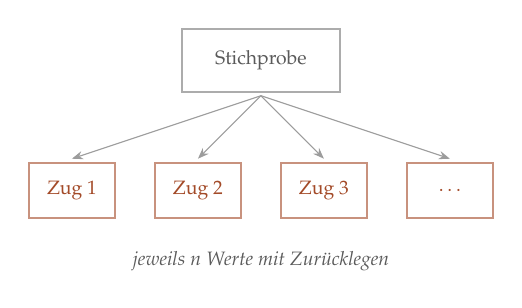
\begin{tikzpicture}[scale=1.0]
\draw[grau!50, line width=0.8pt] (-1.0,1.2) rectangle (1.0,2.0);
\node[font=\scriptsize, color=grau] at (0,1.6) {Stichprobe};
\foreach \i/\x in {0/-2.4, 1/-0.8, 2/0.8, 3/2.4} {
  \draw[akzent!60, line width=0.7pt] (\x-0.55,-0.4) rectangle (\x+0.55,0.3);
  \draw[grau!60, -{Stealth[length=4pt]}] (0,1.15) -- (\x,0.35);
}
\node[font=\scriptsize, color=akzent] at (-2.4,-0.05) {Zug 1};
\node[font=\scriptsize, color=akzent] at (-0.8,-0.05) {Zug 2};
\node[font=\scriptsize, color=akzent] at (0.8,-0.05) {Zug 3};
\node[font=\scriptsize, color=akzent] at (2.4,-0.05) {$\ldots$};
\node[font=\scriptsize\itshape, color=grau] at (0,-0.95) {jeweils $n$ Werte mit Zurücklegen};
\end{tikzpicture}
\end{center}

\schritt{Warum mit Zurücklegen}
Zöge man ohne Zurücklegen, so bekäme man jedes Mal dieselbe Stichprobe zurück. Das Zurücklegen erzeugt die Variabilität, die das wiederholte Ziehen aus der Grundgesamtheit gehabt hätte.
\end{merksatz}

\begin{merksatz}
\boxtitel{Der Bootstrap für MOBIL}
Wir ziehen $20\,000$ Mal je sechs Werte aus Gruppe A und sechs aus Gruppe B --- jeweils mit Zurücklegen --- und berechnen die Differenz der Mittelwerte.

\schritt{Das Ergebnis}
\begin{center}
\renewcommand{\arraystretch}{1.48}
\begin{tabular}{@{}P{3.2cm}P{2.6cm}P{2.2cm}@{}}
\toprule
\textbf{Verfahren} & \textbf{$95\,\%$-Intervall} & \\
\midrule
$t$-Intervall & $[1{,}93;\ 14{,}40]$ & \\
Bootstrap-Perzentil & $[3{,}33;\ 13{,}33]$ & \\
\bottomrule
\end{tabular}
\end{center}

Das Bootstrap-Intervall besteht aus dem $2{,}5$-- und dem $97{,}5$-Prozent-Quantil der $20\,000$ simulierten Differenzen.

\schritt{Der Vergleich}
Die beiden Intervalle stimmen in der Größenordnung überein. Das Bootstrap-Intervall ist etwas enger --- bei $n=6$ ist es dafür bekannt, das Niveau leicht zu verfehlen.

\begin{center}
\begin{minipage}{0.88\textwidth}
\kursiv{Bei sechs Werten je Gruppe gibt es nur $6^6 = 46\,656$ verschiedene Bootstrap-Stichproben, und viele davon bestehen aus wenigen wiederholten Werten. Der Bootstrap braucht eine Stichprobe, die die Grundgesamtheit einigermaßen abbildet --- bei $n = 6$ tut sie das kaum. Als Faustregel gilt $n \ge 20$ bis $30$.}
\end{minipage}
\end{center}
\end{merksatz}

\begin{merksatz}
\boxtitel{Wofür der Bootstrap unersetzlich ist}
Für den Mittelwert gibt es Formeln. Für viele andere Größen nicht.

\begin{center}
\renewcommand{\arraystretch}{1.5}
\begin{tabular}{@{}P{3.2cm}P{5.4cm}@{}}
\toprule
\textbf{Median} & Kein einfacher Standardfehler; der Bootstrap liefert ihn.\\
\textbf{Quotienten} & Verhältnisse zweier Mittelwerte.\\
\textbf{Korrelation} & Ihre Verteilung ist schief und hängt vom wahren Wert ab.\\
\textbf{Zusammen\-gesetztes} & Etwa \enquote{der Unterschied der Mediane, geteilt durch die Spannweite}.\\
\bottomrule
\end{tabular}
\end{center}

\schritt{Ein Beispiel}
Für den Median der Gruppe B ergibt der Bootstrap das Intervall
\[ [\,14{,}5\ ;\ 22{,}0\,] \ \text{Stunden} \]
bei einem Punktschätzer von $17{,}5$. Eine Formel dafür gibt es nicht --- der Bootstrap braucht keine.

\begin{center}
\begin{minipage}{0.88\textwidth}
\kursiv{Man sieht an den Zahlen auch die Grenze: Die Grenzen sind $14{,}5$ und $22{,}0$, also Mittelwerte je zweier vorhandener Datenpunkte. Der Bootstrap kann nur Werte erzeugen, die sich aus der Stichprobe zusammensetzen lassen --- er ist bei Medianen und kleinen $n$ merklich grobkörnig.}
\end{minipage}
\end{center}
\end{merksatz}

\begin{warnung}
\boxtitelr{Was der Bootstrap nicht kann}
\begin{center}
\renewcommand{\arraystretch}{1.5}
\begin{tabular}{@{}P{2.6cm}P{6.0cm}@{}}
\toprule
\textbf{Eine schlechte Stichprobe reparieren} & War die Auswahl verzerrt, so ist es auch jede Bootstrap-Stichprobe. Das Verfahren vervielfältigt den Fehler.\\
\textbf{Extremwerte} & Für Maximum und Minimum versagt er grundsätzlich --- die Bootstrap-Stichprobe kann nie größere Werte enthalten als die ursprüngliche.\\
\textbf{Abhängigkeit} & Bei Zeitreihen oder Mehrebenendaten muss man blockweise ziehen, nicht einzeln.\\
\bottomrule
\end{tabular}
\end{center}

\begin{center}
\begin{minipage}{0.88\textwidth}
\kursiv{Die erste Zeile ist die wichtigste. Der Bootstrap schätzt die Streuung eines Schätzers, nicht seine Verzerrung durch eine schiefe Auswahl. Wer die falschen Leute befragt hat, bekommt ein enges Intervall um den falschen Wert.}
\end{minipage}
\end{center}
\end{warnung}

\section{Übungsaufgaben}

\begin{aufgabe}
\boxtitel{Aufgabe 9.1 --- Mann-Whitney für die Schmerzwerte}
Führen Sie den Test für \code{NRS24} durch: Gruppe A $= 5, 3, 6, 4, 7, 5$ und Gruppe B $= 3, 2, 4, 3, 5, 2$.

\loesung
\schritt{Schritt 1 --- Gemeinsam sortieren und Ränge vergeben}
Sortiert: $2, 2, 3, 3, 3, 4, 4, 5, 5, 5, 6, 7$.

\begin{center}
{\small
\renewcommand{\arraystretch}{1.35}
\begin{tabular}{@{}P{1.2cm}P{2.0cm}P{1.8cm}P{2.4cm}@{}}
\toprule
\textbf{Wert} & \textbf{Plätze} & \textbf{Rang} & \textbf{Gruppen}\\
\midrule
$2$ & $1, 2$ & $1{,}5$ & B, B\\
$3$ & $3,4,5$ & $4$ & A, B, B\\
$4$ & $6,7$ & $6{,}5$ & A, B\\
$5$ & $8,9,10$ & $9$ & A, A, B\\
$6$ & $11$ & $11$ & A\\
$7$ & $12$ & $12$ & A\\
\bottomrule
\end{tabular}}
\end{center}

\schritt{Schritt 2 --- Rangsummen}
Gruppe A hat die Werte $5, 3, 6, 4, 7, 5$ mit den Rängen $9, 4, 11, 6{,}5, 12, 9$:
\[ R_A = 9 + 4 + 11 + 6{,}5 + 12 + 9 = 51{,}5 \]
Gruppe B hat $3, 2, 4, 3, 5, 2$ mit den Rängen $4, 1{,}5, 6{,}5, 4, 9, 1{,}5$:
\[ R_B = 4 + 1{,}5 + 6{,}5 + 4 + 9 + 1{,}5 = 26{,}5 \]

\schritt{Probe}
\[ 51{,}5 + 26{,}5 = 78 = \frac{12 \cdot 13}{2} . \quad \checkmark \]

\schritt{Schritt 3 --- Die Prüfgrößen}
\[ U_A = 51{,}5 - 21 = 30{,}5, \qquad U_B = 26{,}5 - 21 = 5{,}5 \]
Probe: $30{,}5 + 5{,}5 = 36$. \checkmark

\schritt{Schritt 4 --- Entscheidung}
$U = 5{,}5$. Die kritische Schranke lautet $U \le 5$.

$5{,}5 > 5$: \textbf{nicht signifikant.} Der exakte $p$-Wert liegt bei etwa $0{,}058$.

\schritt{Schritt 5 --- Der Vergleich mit dem $t$-Test}
\begin{center}
\renewcommand{\arraystretch}{1.48}
\begin{tabular}{@{}P{3.0cm}P{2.0cm}P{2.6cm}@{}}
\toprule
& $p$ & \\
\midrule
$t$-Test (Aufgabe 7.1) & $0{,}034$ & \textcolor{akzent}{signifikant}\\
Mann-Whitney & $0{,}058$ & \textcolor{gruen}{nicht signifikant}\\
\bottomrule
\end{tabular}
\end{center}

\schritt{Schritt 6 --- Welches Ergebnis gilt?}
Die NRS ist ordinalskaliert. Nach Kapitel~1 ist der Mittelwert dort kodierungsabhängig, die Ränge sind es nicht.

\begin{center}
\begin{minipage}{0.88\textwidth}
\kursiv{Das spricht für den Mann-Whitney-Test --- und damit dafür, das Ergebnis als \kursiv{nicht nachgewiesen} zu berichten. Die vielen Bindungen (nur sechs verschiedene Werte auf zwölf Beobachtungen) schwächen den Rangtest zusätzlich; ein Teil des Unterschieds zwischen $0{,}034$ und $0{,}058$ geht darauf zurück.}
\end{minipage}
\end{center}

\schritt{Was man daraus lernt}
Die Wahl des Verfahrens entscheidet hier über die Schlussfolgerung. Genau deshalb muss sie \kursiv{vor} der Auswertung festgelegt werden --- sonst wählt man das Verfahren, das das gewünschte Ergebnis liefert. Kapitel~15 nennt diese Praxis beim Namen.
\end{aufgabe}

\begin{aufgabe}
\boxtitel{Aufgabe 9.2 --- Einen Permutationstest von Hand}
Zwei Gruppen mit je drei Werten: $A = 10, 12, 14$ und $B = 5, 7, 9$. Führen Sie den Permutationstest für die Differenz der Mittelwerte vollständig durch.

\loesung
\schritt{Schritt 1 --- Die beobachtete Differenz}
\[ \MW_A = \frac{36}{3} = 12, \qquad \MW_B = \frac{21}{3} = 7, \qquad d = 5{,}0 \]

\schritt{Schritt 2 --- Die Anzahl der Aufteilungen}
\[ \binom{6}{3} = 20 . \]

\schritt{Schritt 3 --- Alle durchgehen}
Die sechs Werte lauten $5, 7, 9, 10, 12, 14$ mit Gesamtsumme $57$. Für eine Aufteilung mit A-Summe $S$ ist
\[ d = \frac{S}{3} - \frac{57-S}{3} = \frac{2S - 57}{3} . \]
Es genügt also, die A-Summen aufzulisten.

\begin{center}
{\small
\renewcommand{\arraystretch}{1.3}
\begin{tabular}{@{}P{2.6cm}P{1.2cm}P{1.6cm}P{1.6cm}@{}}
\toprule
\textbf{Gruppe A} & $S$ & $d$ & $|d| \ge 5$?\\
\midrule
$5,7,9$ & $21$ & $-5{,}00$ & \textcolor{akzent}{ja}\\
$5,7,10$ & $22$ & $-4{,}33$ & nein\\
$5,7,12$ & $24$ & $-3{,}00$ & nein\\
$5,7,14$ & $26$ & $-1{,}67$ & nein\\
$5,9,10$ & $24$ & $-3{,}00$ & nein\\
$5,9,12$ & $26$ & $-1{,}67$ & nein\\
$5,9,14$ & $28$ & $-0{,}33$ & nein\\
$5,10,12$ & $27$ & $-1{,}00$ & nein\\
$5,10,14$ & $29$ & $0{,}33$ & nein\\
$5,12,14$ & $31$ & $1{,}67$ & nein\\
$7,9,10$ & $26$ & $-1{,}67$ & nein\\
$7,9,12$ & $28$ & $-0{,}33$ & nein\\
$7,9,14$ & $30$ & $1{,}00$ & nein\\
$7,10,12$ & $29$ & $0{,}33$ & nein\\
$7,10,14$ & $31$ & $1{,}67$ & nein\\
$7,12,14$ & $33$ & $3{,}00$ & nein\\
$9,10,12$ & $31$ & $1{,}67$ & nein\\
$9,10,14$ & $33$ & $3{,}00$ & nein\\
$9,12,14$ & $35$ & $4{,}33$ & nein\\
$10,12,14$ & $36$ & $\mathbf{5{,}00}$ & \textcolor{akzent}{\textbf{ja}}\\
\bottomrule
\end{tabular}}
\end{center}

\schritt{Schritt 4 --- Abzählen}
Genau $2$ von $20$ Aufteilungen erreichen $|d| \ge 5{,}0$: die beobachtete und ihr Spiegelbild.

\[ p = \frac{2}{20} = \mathbf{0{,}10} . \]

\schritt{Schritt 5 --- Die Deutung}
Nicht signifikant --- obwohl sich die beiden Gruppen \kursiv{vollständig} trennen: Jeder A-Wert ist größer als jeder B-Wert.

\begin{center}
\begin{minipage}{0.88\textwidth}
\kursiv{Das ist die Grenze des Verfahrens bei kleinen Zahlen. Der kleinstmögliche zweiseitige $p$-Wert beträgt hier $2/20 = 0{,}10$. Mit je drei Beobachtungen kann kein Permutationstest signifikant werden --- so vollständig die Trennung auch ausfällt.}
\end{minipage}
\end{center}

\schritt{Schritt 6 --- Ab wann es geht}
\begin{center}
\renewcommand{\arraystretch}{1.45}
\begin{tabular}{@{}P{2.0cm}P{2.0cm}P{2.6cm}@{}}
\toprule
$n$ je Gruppe & $\binom{2n}{n}$ & \textbf{kleinstes $p$}\\
\midrule
$3$ & $20$ & $0{,}100$\\
$4$ & $70$ & $0{,}029$\\
$5$ & $252$ & $0{,}0079$\\
$6$ & $924$ & $0{,}0022$\\
\bottomrule
\end{tabular}
\end{center}

Ab vier je Gruppe ist Signifikanz überhaupt erst möglich.
\end{aufgabe}

\begin{aufgabe}
\boxtitel{Aufgabe 9.3 --- Wann welches Verfahren?}
Ordnen Sie den folgenden Lagen ein Verfahren zu und begründen Sie.
\begin{center}
{\small
\renewcommand{\arraystretch}{1.4}
\begin{tabular}{@{}P{0.8cm}P{7.6cm}@{}}
\toprule
(a) & Liegedauer in zwei Kliniken, je $n=200$, stark rechtsschief.\\
(b) & Zufriedenheit auf einer Skala $1$--$5$, zwei Gruppen zu je $30$.\\
(c) & Konfidenzintervall für den Median der Behandlungskosten, $n=50$.\\
(d) & Randomisierte Studie, $n=15$ je Gruppe, Endpunkt stetig.\\
\bottomrule
\end{tabular}}
\end{center}

\loesung
\schritt{(a) --- $t$-Test ist vertretbar}
Bei $n = 200$ je Gruppe trägt der zentrale Grenzwertsatz auch bei starker Schiefe. Die Mittelwerte sind dann gut normalverteilt.

\begin{center}
\begin{minipage}{0.86\textwidth}
\kursiv{Die Frage ist eher, ob der \kursiv{Mittelwert} die richtige Kennzahl ist. Bei stark schiefen Kosten- oder Dauerdaten sagt der Median oft mehr über den typischen Fall aus --- und dann ist die Frage nicht, welcher Test, sondern welcher Parameter.}
\end{minipage}
\end{center}

\schritt{(b) --- Mann-Whitney}
Fünfstufige Skala, also ordinal. Bei $n = 30$ je Gruppe gibt es viele Bindungen; man rechnet mit der Bindungskorrektur, die jedes Programm anwendet.

Eine Alternative ist die ordinale Regression (Kapitel~11), die zusätzlich einen deutbaren Effektschätzer liefert.

\schritt{(c) --- Bootstrap}
Für den Median gibt es keine brauchbare Formel. Bei $n = 50$ ist der Bootstrap gut anwendbar.

\schritt{(d) --- Permutationstest}
Hier ist er die erste Wahl, und zwar aus einem besonderen Grund: Die Randomisierung \kursiv{erzeugt} die Austauschbarkeit, die das Verfahren voraussetzt. Man muss über die Verteilung der Daten gar nichts annehmen.

Bei $n=15$ je Gruppe gibt es $\binom{30}{15} \approx 1{,}55 \cdot 10^8$ Aufteilungen --- zu viele zum Abzählen, aber problemlos für eine Monte-Carlo-Näherung mit $100\,000$ Ziehungen.

\schritt{Die Zusammenfassung}
\begin{center}
\renewcommand{\arraystretch}{1.45}
\begin{tabular}{@{}P{1.0cm}P{3.0cm}P{4.0cm}@{}}
\toprule
& \textbf{Verfahren} & \textbf{Grund}\\
\midrule
(a) & $t$-Test & $n$ groß genug\\
(b) & Mann-Whitney & ordinal\\
(c) & Bootstrap & keine Formel\\
(d) & Permutation & Randomisierung\\
\bottomrule
\end{tabular}
\end{center}
\end{aufgabe}

\begin{geschichte}
\boxtitelg{Ein Chemiker, zwei Statistiker und ein Schnürsenkel}
\Person{Frank Wilcoxon} (1892--1965) war Chemiker bei einer Agrarfirma in Connecticut. Er wertete Versuche mit Pflanzenschutzmitteln aus und suchte ein Verfahren, das ohne Verteilungsannahme auskommt.

Seine Arbeit von 1945 umfasst drei Seiten und enthält beide nach ihm benannten Tests. Er veröffentlichte sie in einem neu gegründeten, kaum beachteten Mitteilungsblatt; der Aufsatz wurde zu einem der meistzitierten der Statistik.

Zwei Jahre später leiteten \Person{Henry Mann} und \Person{Donald Whitney} unabhängig davon dasselbe Verfahren her --- in anderer Schreibweise und mit vollständiger Theorie. Daher die beiden Namen für einen Test.

\begin{center}
\begin{minipage}{0.9\textwidth}
\kursiv{Der Bootstrap ist jünger. \Person{Bradley Efron} stellte ihn 1979 vor; der Name geht auf die Redewendung zurück, sich am eigenen Schnürsenkel aus dem Sumpf zu ziehen --- die deutsche Entsprechung wäre der Münchhausen-Zopf. Gemeint ist das scheinbar Unmögliche: aus einer einzigen Stichprobe die Streuung über viele Stichproben zu gewinnen.}
\end{minipage}
\end{center}

Das Verfahren war nur denkbar, weil Rechenzeit billig geworden war. Efron selbst nannte es ein Beispiel dafür, wie technische Möglichkeiten die Theorie verändern: Was man vorher analytisch herleiten musste, konnte man nun ausprobieren.
\end{geschichte}

\begin{forschung}
\boxtitelp{Rangtests, Permutation und was sich durchsetzt}
\begin{center}
{\small
\renewcommand{\arraystretch}{1.45}
\begin{tabular}{@{}P{2.6cm}P{5.6cm}@{}}
\toprule
\textbf{Machtverlust} & Sind die Daten tatsächlich normalverteilt, verliert Mann-Whitney gegenüber dem $t$-Test nur etwa $5\,\%$ an Macht --- ein erstaunlich kleiner Preis.\\
\textbf{Machtgewinn} & Bei schweren Rändern kann er dem $t$-Test deutlich überlegen sein.\\
\textbf{Der Effektschätzer} & Die Überlegenheitswahrscheinlichkeit setzt sich als Berichtsgröße durch; sie heißt auch \enquote{common language effect size}.\\
\bottomrule
\end{tabular}}
\end{center}

Der Wert $5\,\%$ ist bemerkenswert: Er bedeutet, dass man mit dem Rangtest bei normalverteilten Daten etwa $5\,\%$ mehr Personen braucht --- und dafür gegen Verletzungen der Annahme geschützt ist. Die theoretische Untergrenze liegt bei $1 - 3/\pi \approx 4{,}5\,\%$ und wird bei Normalverteilung fast erreicht.

\schritt{Die Bewegung zur Permutation}
In der methodischen Literatur wächst die Auffassung, dass der Permutationstest in randomisierten Studien das eigentlich angemessene Verfahren ist --- weil seine Voraussetzung durch das Studiendesign selbst geschaffen wird und nicht angenommen werden muss.

\begin{center}
\begin{minipage}{0.88\textwidth}
\kursiv{Durchgesetzt hat er sich nicht. Die Gründe sind praktisch: Rechenaufwand bei großen Datensätzen, fehlende Voreinstellungen in Auswertungsprogrammen, und die Schwierigkeit, aus einem Permutationstest ein Konfidenzintervall zu gewinnen --- was möglich, aber umständlich ist.}
\end{minipage}
\end{center}
\end{forschung}

\begin{merksatz}
\boxtitel{Was Sie jetzt können}
\begin{center}
\renewcommand{\arraystretch}{1.5}
\begin{tabular}{@{}P{3.0cm}P{5.6cm}@{}}
\toprule
\textbf{Vorzeichentest} & und warum er bei $n \le 5$ nie signifikant wird\\
\textbf{Wilcoxon} & Ränge der Beträge\\
\textbf{Mann-Whitney} & $U$, die Proben, und was er wirklich prüft\\
\textbf{Permutation} & exakt, ohne Verteilungsannahme\\
\textbf{Bootstrap} & für Größen ohne Formel --- und seine drei Grenzen\\
\bottomrule
\end{tabular}
\end{center}

\begin{center}
\begin{minipage}{0.88\textwidth}
\kursiv{Damit endet Teil~III. Ab Kapitel~10 geht es nicht mehr um den Vergleich zweier Gruppen, sondern um den Zusammenhang mehrerer Größen.}
\end{minipage}
\end{center}
\end{merksatz}

\part{Modelle}

\chapter{Lineare Regression}

\section{Von der Kennzahl zur Funktion}

Kapitel~3 fasste den Zusammenhang zweier Merkmale in eine Zahl: die Korrelation. Sie sagt, wie eng die Punkte an einer Geraden liegen --- aber nicht, welche Gerade das ist.

\begin{merksatz}
\boxtitel{Was die Regression zusätzlich leistet}
\begin{center}
\renewcommand{\arraystretch}{1.5}
\begin{tabular}{@{}P{2.4cm}P{6.2cm}@{}}
\toprule
\textbf{Korrelation} & Wie eng? Eine Zahl zwischen $-1$ und $1$, einheitenfrei, symmetrisch in $x$ und $y$.\\
\textbf{Regression} & Wie genau? Eine Gerade mit Steigung in Einheiten, \kursiv{unsymmetrisch}: $y$ aus $x$ ist etwas anderes als $x$ aus $y$.\\
\bottomrule
\end{tabular}
\end{center}

\begin{center}
\begin{minipage}{0.88\textwidth}
\kursiv{Die Unsymmetrie ist wesentlich. Man muss entscheiden, welche Größe die \kursiv{erklärende} und welche die \kursiv{erklärte} ist --- und diese Entscheidung folgt nicht aus den Daten.}
\end{minipage}
\end{center}
\end{merksatz}

\begin{definition}
\boxtitelm{Definition 10.1 --- das Modell}
\[ y_i \;=\; \alpha + \beta\,x_i + \varepsilon_i \]
mit
\begin{center}
\renewcommand{\arraystretch}{1.5}
\begin{tabular}{@{}P{1.6cm}P{6.8cm}@{}}
\toprule
$\alpha$ & Achsenabschnitt: der Wert von $y$ bei $x = 0$\\
$\beta$ & Steigung: die Änderung von $y$ je Einheit von $x$\\
$\varepsilon_i$ & Störgröße: alles, was die Gerade nicht erklärt\\
\bottomrule
\end{tabular}
\end{center}
\end{definition}

\begin{merksatz}
\boxtitel{Die Voraussetzungen --- ausdrücklich aufgezählt}
\begin{center}
{\small
\renewcommand{\arraystretch}{1.52}
\begin{tabular}{@{}P{2.8cm}P{5.8cm}@{}}
\toprule
\textbf{Linearität} & Der Zusammenhang ist tatsächlich geradlinig.\\
\textbf{Unabhängig\-keit} & Die $\varepsilon_i$ beeinflussen einander nicht.\\
\textbf{Gleiche Streuung} & $\Var[\varepsilon_i] = \sigma^2$ für alle $i$ --- die Streuung hängt nicht von $x$ ab.\\
\textbf{Normal\-verteilung} & Nur für Tests und Intervalle nötig, nicht für die Schätzung selbst.\\
\textbf{$x$ ohne Fehler} & Die erklärende Größe gilt als exakt bekannt.\\
\bottomrule
\end{tabular}}
\end{center}

\begin{center}
\begin{minipage}{0.88\textwidth}
\kursiv{Die letzte Zeile wird fast immer verletzt --- auch die NRS-Angabe ist eine Messung mit Fehler. Die Folge ist ein systematischer Fehler: Die geschätzte Steigung wird zu \kursiv{flach}. Abschnitt 10.7 kommt darauf zurück.}
\end{minipage}
\end{center}
\end{merksatz}

\section{Die Methode der kleinsten Quadrate}

\begin{merksatz}
\boxtitel{Satz 10.2 --- die Schätzformeln}
Die Gerade, die
\[ S(a,b) = \sum_{i=1}^n \bigl(y_i - a - b\,x_i\bigr)^2 \]
minimiert, hat die Parameter
\[ b = \frac{\sum_i (x_i-\MW)(y_i-\overline y)}{\sum_i (x_i-\MW)^2}, \qquad a = \overline y - b\,\MW . \]
\end{merksatz}

\begin{merksatz}
\boxtitel{Beweis}
\schritt{Schritt 1 --- Nach $a$ ableiten}
\[ \frac{\partial S}{\partial a} = \sum_i 2\bigl(y_i - a - bx_i\bigr)\cdot(-1) = -2\sum_i \bigl(y_i - a - bx_i\bigr) \]
Null setzen:
\[ \sum_i y_i - na - b\sum_i x_i = 0 \]
Durch $n$ teilen:
\[ \overline y - a - b\,\MW = 0 \quad\Longrightarrow\quad a = \overline y - b\,\MW . \]

\schritt{Was das schon aussagt}
Umgestellt: $\overline y = a + b\,\MW$. Die Gerade geht also stets durch den Punkt $(\MW, \overline y)$ --- durch den Schwerpunkt der Punktwolke. Das gilt \kursiv{unabhängig} von der Steigung.

\schritt{Schritt 2 --- Nach $b$ ableiten}
\[ \frac{\partial S}{\partial b} = -2\sum_i x_i\bigl(y_i - a - bx_i\bigr) \;\stackrel{!}{=}\; 0 \]

\schritt{Schritt 3 --- $a$ einsetzen}
Mit $a = \overline y - b\MW$ wird der Klammerausdruck zu
\[ y_i - \overline y + b\MW - bx_i = (y_i - \overline y) - b(x_i - \MW) . \]
Also
\[ \sum_i x_i\Bigl[(y_i-\overline y) - b(x_i-\MW)\Bigr] = 0 . \]

\schritt{Schritt 4 --- Ein nützlicher Trick}
Wir dürfen $x_i$ durch $x_i - \MW$ ersetzen. Denn der zusätzliche Term wäre
\[ \MW\sum_i\Bigl[(y_i-\overline y) - b(x_i-\MW)\Bigr] = \MW\Bigl[\underbrace{\sum_i(y_i-\overline y)}_{=0} - b\underbrace{\sum_i(x_i-\MW)}_{=0}\Bigr] = 0 \]
nach Satz 2.3. Also gilt gleichbedeutend
\[ \sum_i (x_i-\MW)\Bigl[(y_i-\overline y) - b(x_i-\MW)\Bigr] = 0 . \]

\schritt{Schritt 5 --- Auflösen}
\[ \sum_i (x_i-\MW)(y_i-\overline y) - b\sum_i (x_i-\MW)^2 = 0 \]
\[ b = \frac{\sum_i (x_i-\MW)(y_i-\overline y)}{\sum_i (x_i-\MW)^2} . \qquad \blacksquare \]

\schritt{Dass es ein Minimum ist}
$S$ ist eine Summe von Quadraten, also nach oben unbeschränkt und nach unten durch null begrenzt. Die einzige Stelle mit verschwindenden Ableitungen muss daher das Minimum sein.
\end{merksatz}

\begin{merksatz}
\boxtitel{Der Zusammenhang mit der Korrelation}
Der Zähler von $b$ ist derselbe wie der von $r$. Es gilt
\[ b = r \cdot \frac{s_y}{s_x} . \]

\schritt{Nachrechnen}
\[ r\cdot\frac{s_y}{s_x} = \frac{\sum(x-\MW)(y-\overline y)}{\sqrt{\sum(x-\MW)^2}\sqrt{\sum(y-\overline y)^2}} \cdot \frac{\sqrt{\sum(y-\overline y)^2}}{\sqrt{\sum(x-\MW)^2}} = \frac{\sum(x-\MW)(y-\overline y)}{\sum(x-\MW)^2} = b . \quad \checkmark \]

\begin{center}
\begin{minipage}{0.88\textwidth}
\kursiv{Korrelation und Steigung tragen dieselbe Auskunft, nur verschieden normiert. Die Korrelation ist einheitenfrei, die Steigung hat die Einheit \enquote{$y$-Einheit je $x$-Einheit} --- und ist deshalb die deutbarere Größe.}
\end{minipage}
\end{center}
\end{merksatz}

\section{Die MOBIL-Daten}

\begin{merksatz}
\boxtitel{Die Gerade bestimmen}
Wir erklären die Mobilisationszeit aus dem Schmerzwert. Aus Kapitel~3 liegen alle Summen vor:
\[ \MW = 4{,}0833, \quad \overline y = 22{,}0833 \]
\[ \sum(x-\MW)^2 = 26{,}917, \quad \sum(x-\MW)(y-\overline y) = 103{,}917 \]

\schritt{Die Steigung}
\[ b = \frac{103{,}917}{26{,}917} = 3{,}861 \]

\schritt{Der Achsenabschnitt}
\[ a = 22{,}0833 - 3{,}861 \cdot 4{,}0833 = 22{,}0833 - 15{,}765 = 6{,}319 \]

\schritt{Die Gleichung}
\[ \hat y = 6{,}32 + 3{,}86\,x \]

\schritt{Die Deutung --- Zeile für Zeile}
\begin{center}
{\small
\renewcommand{\arraystretch}{1.5}
\begin{tabular}{@{}P{2.0cm}P{6.4cm}@{}}
\toprule
$b = 3{,}86$ & Je NRS-Punkt mehr dauert die Mobilisation im Mittel $3{,}9$ Stunden länger.\\
$a = 6{,}32$ & \textcolor{akzent}{Vorhergesagte Mobilisationszeit bei Schmerzwert null --- eine Hochrechnung über den Datenbereich hinaus.}\\
\bottomrule
\end{tabular}}
\end{center}

\begin{center}
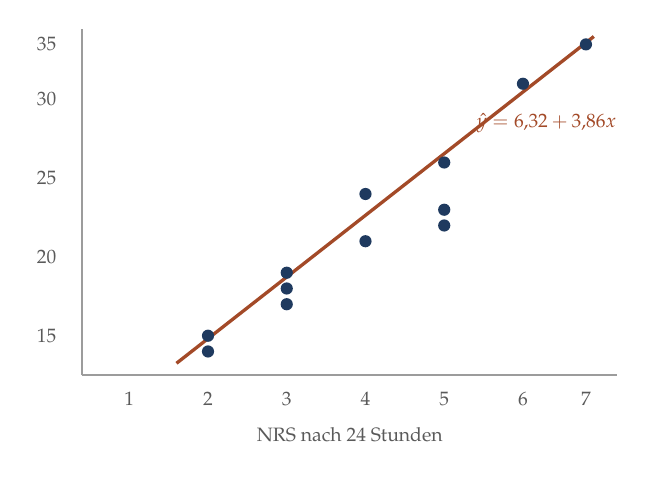
\begin{tikzpicture}[scale=1.0]
\draw[grau!60, line width=0.7pt] (0,0) -- (6.8,0);
\draw[grau!60, line width=0.7pt] (0,0) -- (0,4.4);
\foreach \x/\lab in {0.6/1, 1.6/2, 2.6/3, 3.6/4, 4.6/5, 5.6/6, 6.4/7}
  \node[font=\scriptsize, color=grau] at (\x,-0.3) {\lab};
\foreach \y/\lab in {0.5/15, 1.5/20, 2.5/25, 3.5/30, 4.2/35}
  \node[font=\scriptsize, color=grau] at (-0.45,\y) {\lab};
\draw[akzent, line width=1.2pt] (1.2,0.15) -- (6.5,4.3);
\fill[tief] (4.6,2.7) circle (2.2pt);
\fill[tief] (2.6,1.3) circle (2.2pt);
\fill[tief] (5.6,3.7) circle (2.2pt);
\fill[tief] (3.6,2.3) circle (2.2pt);
\fill[tief] (6.4,4.2) circle (2.2pt);
\fill[tief] (4.6,1.9) circle (2.2pt);
\fill[tief] (2.6,1.1) circle (2.2pt);
\fill[tief] (1.6,0.5) circle (2.2pt);
\fill[tief] (3.6,1.7) circle (2.2pt);
\fill[tief] (2.6,0.9) circle (2.2pt);
\fill[tief] (4.6,2.1) circle (2.2pt);
\fill[tief] (1.6,0.3) circle (2.2pt);
\node[font=\scriptsize, color=grau] at (3.4,-0.75) {NRS nach 24 Stunden};
\node[font=\scriptsize, color=akzent] at (5.9,3.2) {$\hat y = 6{,}32 + 3{,}86x$};
\end{tikzpicture}
\end{center}
\end{merksatz}

\begin{warnung}
\boxtitelr{Der Achsenabschnitt ist hier bedeutungslos}
Der kleinste beobachtete NRS-Wert beträgt $2$. Die Gerade bei $x = 0$ auszuwerten heißt, weit außerhalb des Datenbereichs vorherzusagen.

\begin{center}
\begin{minipage}{0.9\textwidth}
\textbf{Eine Regressionsgerade gilt nur im Bereich der beobachteten $x$-Werte.} Außerhalb ist sie eine Behauptung ohne Datengrundlage.
\end{minipage}
\end{center}

\schritt{Ein Ausweg}
Verschiebt man die erklärende Größe auf ihren Mittelwert --- man rechnet mit $x - \MW$ statt mit $x$ ---, so wird der Achsenabschnitt zu $\overline y = 22{,}08$ und bedeutet: die vorhergesagte Zeit bei durchschnittlichem Schmerzwert. Das ist eine sinnvolle Größe. Die Steigung ändert sich dabei nicht.
\end{warnung}

\section{Wie gut passt die Gerade?}

\begin{definition}
\boxtitelm{Definition 10.3 --- Residuum und Bestimmtheitsmaß}
Das \Begriff{Residuum} der $i$-ten Beobachtung ist
\[ e_i = y_i - \hat y_i . \]
Die Streuung zerlegt sich in
\[ \underbrace{\sum_i (y_i-\overline y)^2}_{SS_{\text{gesamt}}} = \underbrace{\sum_i (\hat y_i - \overline y)^2}_{SS_{\text{erklärt}}} + \underbrace{\sum_i e_i^2}_{SS_{\text{Rest}}} , \]
und das \Begriff{Bestimmtheitsmaß} ist
\[ R^2 = \frac{SS_{\text{erklärt}}}{SS_{\text{gesamt}}} = 1 - \frac{SS_{\text{Rest}}}{SS_{\text{gesamt}}} . \]
\end{definition}

\begin{merksatz}
\boxtitel{Bei einfacher Regression gilt $R^2 = r^2$}
Für die MOBIL-Daten war $r = 0{,}9605$, also
\[ R^2 = 0{,}9605^2 = 0{,}9225 . \]

\schritt{Die Rechnung zur Probe}
\[ SS_{\text{Rest}} = SS_{\text{gesamt}}\,(1-R^2) = 434{,}917 \cdot 0{,}0775 = 33{,}70 \]

\schritt{Die Deutung}
$92{,}3\,\%$ der Streuung der Mobilisationszeiten lassen sich durch den Schmerzwert erklären.

\begin{center}
\begin{minipage}{0.88\textwidth}
\kursiv{Das Wort \enquote{erklären} ist hier rein rechnerisch gemeint --- es besagt \kursiv{nicht}, dass der Schmerz die Ursache ist. Alle vier Erklärungen aus Kapitel~3 bleiben möglich.}
\end{minipage}
\end{center}
\end{merksatz}

\begin{warnung}
\boxtitelr{Was $R^2$ nicht sagt}
\begin{center}
{\small
\renewcommand{\arraystretch}{1.52}
\begin{tabular}{@{}P{2.4cm}P{6.2cm}@{}}
\toprule
\textbf{Nicht: das Modell ist richtig} & Anscombe~II hat $R^2 = 0{,}67$ bei einem exakt gekrümmten Zusammenhang. Die Gerade ist falsch, $R^2$ merkt es nicht.\\
\textbf{Nicht: die Steigung ist groß} & $R^2$ hängt nicht von der Einheit ab, die Steigung schon.\\
\textbf{Nicht: gut für Vorhersagen} & Bei $R^2 = 0{,}92$ und großer Gesamtstreuung können die Einzelvorhersagen weit danebenliegen.\\
\textbf{Nicht vergleichbar} & Über verschiedene Datensätze hinweg sagt $R^2$ wenig --- es hängt auch davon ab, wie breit die $x$-Werte streuen.\\
\bottomrule
\end{tabular}}
\end{center}

\schritt{Zur letzten Zeile}
Wählt man nur Personen mit NRS zwischen $4$ und $5$ aus, so schrumpft $\sum(x-\MW)^2$ stark --- und $R^2$ fällt, obwohl der Zusammenhang derselbe ist. Ein hohes $R^2$ kann schlicht bedeuten, dass die erklärende Größe breit streute.
\end{warnung}

\section{Tests und Intervalle für die Steigung}

\begin{merksatz}
\boxtitel{Der Standardfehler der Steigung}
\[ \widehat{\mathrm{SE}}(b) = \frac{s_e}{\sqrt{\sum_i (x_i-\MW)^2}} \qquad\text{mit}\qquad s_e^2 = \frac{SS_{\text{Rest}}}{n-2} . \]

\schritt{Warum $n-2$}
Zwei Parameter wurden geschätzt --- $a$ und $b$. Es bleiben $n-2$ freie Abweichungen. Das ist dieselbe Überlegung wie beim $n-1$ in Kapitel~5.

\schritt{Für MOBIL}
\[ s_e^2 = \frac{33{,}70}{12-2} = 3{,}370, \qquad s_e = 1{,}836 \]
\[ \widehat{\mathrm{SE}}(b) = \frac{1{,}836}{\sqrt{26{,}917}} = \frac{1{,}836}{5{,}188} = 0{,}3539 \]

\schritt{Der Test auf $\beta = 0$}
\[ t = \frac{b}{\widehat{\mathrm{SE}}(b)} = \frac{3{,}861}{0{,}3539} = 10{,}91 \]
bei $n-2 = 10$ Freiheitsgraden. Das liegt weit über $t_{10;\,0{,}9995} = 4{,}587$; $p < 0{,}0001$.

\schritt{Das Konfidenzintervall}
\[ 3{,}861 \pm 2{,}228 \cdot 0{,}3539 = 3{,}861 \pm 0{,}789 \quad\Longrightarrow\quad [\,3{,}07\ ;\ 4{,}65\,] \]

\begin{center}
\begin{minipage}{0.88\textwidth}
\kursiv{So berichtet man das Ergebnis: \enquote{Je NRS-Punkt verlängerte sich die Mobilisation um $3{,}9$ Stunden ($95\,\%$-KI $3{,}1$ bis $4{,}7$).} Der $p$-Wert ist dabei die unwichtigste Angabe.}
\end{minipage}
\end{center}

\schritt{Die Bedeutung des Nenners}
$\widehat{\mathrm{SE}}(b)$ enthält $\sum(x-\MW)^2$ im Nenner. Je breiter die $x$-Werte streuen, desto genauer ist die Steigung bestimmt.

Das hat eine praktische Folge für die Versuchsplanung: Will man eine Steigung genau schätzen, wählt man die $x$-Werte möglichst \kursiv{weit auseinander} --- nicht gleichmäßig verteilt.
\end{merksatz}

\section{Residuenanalyse}

\begin{merksatz}
\boxtitel{Was man ansieht}
Man trägt die Residuen $e_i$ gegen die vorhergesagten Werte $\hat y_i$ auf. Bei einem passenden Modell sieht man eine strukturlose Wolke.

\begin{center}
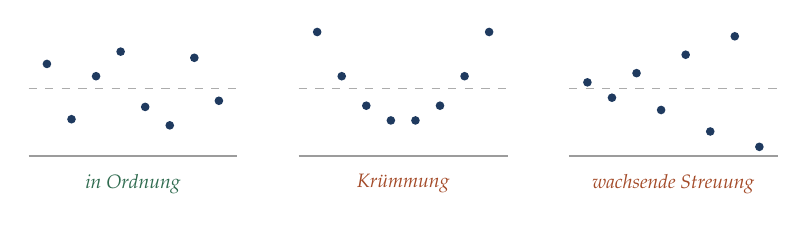
\begin{tikzpicture}[scale=0.78]
% 1 gut
\begin{scope}
\draw[grau!60, line width=0.6pt] (0,-1.1) -- (3.4,-1.1);
\draw[grau!50, dashed, line width=0.6pt] (0,0) -- (3.4,0);
\foreach \x/\y in {0.3/0.4, 0.7/-0.5, 1.1/0.2, 1.5/0.6, 1.9/-0.3, 2.3/-0.6, 2.7/0.5, 3.1/-0.2}
  \fill[tief] (\x,\y) circle (2.0pt);
\node[font=\scriptsize\itshape, color=gruen] at (1.7,-1.55) {in Ordnung};
\end{scope}
% 2 Krümmung
\begin{scope}[xshift=4.4cm]
\draw[grau!60, line width=0.6pt] (0,-1.1) -- (3.4,-1.1);
\draw[grau!50, dashed, line width=0.6pt] (0,0) -- (3.4,0);
\foreach \x in {0.3,0.7,1.1,1.5,1.9,2.3,2.7,3.1}
  \fill[tief] (\x,{0.75*(\x-1.7)*(\x-1.7)-0.55}) circle (2.0pt);
\node[font=\scriptsize\itshape, color=akzent] at (1.7,-1.55) {Krümmung};
\end{scope}
% 3 Trichter
\begin{scope}[xshift=8.8cm]
\draw[grau!60, line width=0.6pt] (0,-1.1) -- (3.4,-1.1);
\draw[grau!50, dashed, line width=0.6pt] (0,0) -- (3.4,0);
\foreach \x/\y in {0.3/0.1, 0.7/-0.15, 1.1/0.25, 1.5/-0.35, 1.9/0.55, 2.3/-0.7, 2.7/0.85, 3.1/-0.95}
  \fill[tief] (\x,\y) circle (2.0pt);
\node[font=\scriptsize\itshape, color=akzent] at (1.7,-1.55) {wachsende Streuung};
\end{scope}
\end{tikzpicture}
\end{center}

\begin{center}
{\small
\renewcommand{\arraystretch}{1.5}
\begin{tabular}{@{}P{2.4cm}P{2.8cm}P{3.0cm}@{}}
\toprule
\textbf{Muster} & \textbf{Bedeutet} & \textbf{Abhilfe}\\
\midrule
strukturlos & \textcolor{gruen}{Modell passt} & ---\\
Krümmung & Linearität verletzt & Term $x^2$, oder Logarithmus\\
Trichter & Streuung hängt von $x$ ab & $y$ logarithmieren, gewichtete Regression\\
Ausreißer & einzelne Punkte & prüfen, nicht löschen\\
\bottomrule
\end{tabular}}
\end{center}

\begin{center}
\begin{minipage}{0.88\textwidth}
\kursiv{Die Residuen summieren sich stets zu null --- das folgt aus Schritt 1 des Beweises von Satz 10.2. Ihre Nullsumme ist daher keine Bestätigung des Modells, sondern eine Eigenschaft der Rechnung.}
\end{minipage}
\end{center}
\end{merksatz}

\begin{warnung}
\boxtitelr{Einflussreiche Punkte}
Ein Punkt kann die Gerade stark beeinflussen, ohne ein großes Residuum zu haben --- gerade weil er die Gerade zu sich hinzieht.

Das ist Anscombe~IV: Der einzelne rechte Punkt bestimmt die Steigung vollständig und liegt trotzdem exakt auf der Geraden.

\begin{center}
\renewcommand{\arraystretch}{1.5}
\begin{tabular}{@{}P{2.8cm}P{5.8cm}@{}}
\toprule
\textbf{Hebel\-wirkung} & Wie weit liegt der $x$-Wert vom Mittel entfernt? Große Hebelwirkung heißt: der Punkt kann viel bewirken.\\
\textbf{Residuum} & Wie weit liegt der $y$-Wert von der Geraden entfernt?\\
\textbf{Einfluss} & Beides zusammen --- gemessen etwa durch den Abstand nach Cook.\\
\bottomrule
\end{tabular}
\end{center}

\begin{center}
\begin{minipage}{0.88\textwidth}
\kursiv{Die Prüfung ist einfach: Man rechnet die Regression ohne den fraglichen Punkt noch einmal. Ändert sich die Steigung erheblich, so beruht das Ergebnis auf einer Beobachtung --- und das gehört in den Bericht.}
\end{minipage}
\end{center}
\end{warnung}

\section{Regression zur Mitte}

Jetzt der Effekt, der der Regression ihren Namen gab --- und der in der Medizin regelmäßig für Wirkungen gehalten wird, die es nicht gibt.

\begin{merksatz}
\boxtitel{Die Rechnung}
Standardisiert man beide Merkmale, so lautet die Regressionsgleichung schlicht
\[ \hat z_y = r \cdot z_x . \]

\schritt{Der Nachweis}
Für standardisierte Größen ist $\MW = \overline y = 0$ und $s_x = s_y = 1$. Nach Abschnitt 10.2 ist dann $b = r \cdot \frac{1}{1} = r$ und $a = 0 - r\cdot 0 = 0$.

\schritt{Die Folgerung}
Ist $|r| < 1$, so gilt $|\hat z_y| < |z_x|$: \textbf{Der vorhergesagte Wert liegt stets näher am Mittelwert als der Ausgangswert.}

\begin{center}
\renewcommand{\arraystretch}{1.48}
\begin{tabular}{@{}P{2.6cm}P{2.2cm}P{2.6cm}@{}}
\toprule
$z_x$ & $r = 0{,}6$ & $\hat z_y$\\
\midrule
$+3{,}0$ & & $+1{,}8$\\
$+1{,}0$ & & $+0{,}6$\\
$-2{,}0$ & & $-1{,}2$\\
\bottomrule
\end{tabular}
\end{center}
\end{merksatz}

\begin{warnung}
\boxtitelr{Die Falle in der Medizin}
\schritt{Der Vorgang}
\begin{center}
\renewcommand{\arraystretch}{1.5}
\begin{tabular}{@{}P{1.0cm}P{7.4cm}@{}}
\toprule
$1$ & Man misst bei vielen Personen den Blutdruck.\\
$2$ & Man wählt diejenigen mit den höchsten Werten für eine Studie aus.\\
$3$ & Man behandelt sie und misst erneut.\\
$4$ & Die Werte sind gesunken. Die Behandlung wirkt --- scheinbar.\\
\bottomrule
\end{tabular}
\end{center}

\schritt{Warum die Werte auch ohne Behandlung sinken}
Ein hoher gemessener Wert entsteht aus zwei Anteilen: dem wahren Blutdruck der Person \kursiv{und} einer zufälligen Abweichung --- Tagesform, Messfehler, Aufregung.

Wählt man die höchsten Werte aus, so wählt man bevorzugt Personen mit einer zufällig \kursiv{nach oben} verschobenen Messung. Bei der zweiten Messung ist diese Abweichung neu gewürfelt und im Mittel null.

\begin{center}
\begin{minipage}{0.9\textwidth}
\textbf{Die Werte sinken also, weil sie ausgewählt wurden --- nicht, weil behandelt wurde.}
\end{minipage}
\end{center}

\schritt{Ein Zahlenbeispiel}
Angenommen, der Blutdruck streut mit $\sigma = 15$, davon $10$ wahre Verschiedenheit und $11{,}2$ Messschwankung. Dann ist die Korrelation zweier Messungen etwa
\[ r = \frac{10^2}{15^2} = 0{,}44 . \]
Wählt man Personen aus, die $2$ Standardabweichungen über dem Mittel liegen, so sagt die Regression für die zweite Messung
\[ \hat z = 0{,}44 \cdot 2 = 0{,}88 \]
voraus --- ein Rückgang um $1{,}12$ Standardabweichungen, also etwa $17$ mmHg, \kursiv{ohne jede Behandlung}.

\begin{center}
\begin{minipage}{0.88\textwidth}
\kursiv{Genau deshalb braucht man eine Kontrollgruppe. Sie durchläuft dieselbe Auswahl und zeigt denselben Rückgang; der Vergleich beider Gruppen misst dann die Behandlung. Kapitel~12 macht daraus ein Gestaltungsprinzip.}
\end{minipage}
\end{center}

\schritt{Wo derselbe Fehler noch auftritt}
\begin{center}
\renewcommand{\arraystretch}{1.5}
\begin{tabular}{@{}P{3.2cm}P{5.4cm}@{}}
\toprule
Laborwerte & Auffällige Werte normalisieren sich beim Nachkontrollieren.\\
Schulleistung & Förderung der Schlechtesten \enquote{wirkt} immer.\\
Qualitäts\-kennzahlen & Die schlechtesten Kliniken verbessern sich im Folgejahr.\\
Schmerzskalen & Wer bei starken Schmerzen behandelt wird, berichtet danach weniger.\\
\bottomrule
\end{tabular}
\end{center}
\end{warnung}

\section{Mehrere erklärende Größen}

\begin{merksatz}
\boxtitel{Das Modell}
\[ y_i = \alpha + \beta_1 x_{i1} + \beta_2 x_{i2} + \cdots + \beta_k x_{ik} + \varepsilon_i \]

\schritt{Die veränderte Deutung}
$\beta_1$ ist nicht mehr \enquote{die Änderung von $y$ je Einheit $x_1$}, sondern

\begin{center}
\begin{minipage}{0.9\textwidth}
\textbf{die Änderung von $y$ je Einheit $x_1$ \kursiv{bei festgehaltenen übrigen Größen}.}
\end{minipage}
\end{center}

Das ist etwas anderes und kann sogar ein anderes Vorzeichen haben als der einfache Zusammenhang.
\end{merksatz}

\begin{warnung}
\boxtitelr{Kollinearität}
Sind zwei erklärende Größen stark miteinander korreliert, so lässt sich ihr Beitrag nicht trennen.

\begin{center}
\renewcommand{\arraystretch}{1.5}
\begin{tabular}{@{}P{2.6cm}P{6.0cm}@{}}
\toprule
\textbf{Das Merkmal} & Große Standardfehler, instabile Koeffizienten, unplausible Vorzeichen.\\
\textbf{Der Grund} & Die Daten enthalten keine Auskunft darüber, welche der beiden Größen wirkt.\\
\textbf{Nicht das Merkmal} & $R^2$ bleibt hoch --- die \kursiv{Vorhersage} leidet nicht.\\
\bottomrule
\end{tabular}
\end{center}

\schritt{Ein Beispiel}
Nimmt man Körpergröße und Armspannweite gemeinsam in ein Modell auf, so sind beide Koeffizienten schlecht bestimmt und können entgegengesetzte Vorzeichen bekommen. Zusammen sagen sie dasselbe vorher wie jede einzeln.

\begin{center}
\begin{minipage}{0.88\textwidth}
\kursiv{Die Abhilfe ist keine statistische: Man entscheidet fachlich, welche Größe gemeint ist, und nimmt eine davon. Verfahren, die automatisch Größen auswählen --- schrittweise Regression ---, gelten heute als problematisch, weil sie die anschließenden $p$-Werte ungültig machen.}
\end{minipage}
\end{center}
\end{warnung}

\begin{warnung}
\boxtitelr{Welche Größen gehören ins Modell?}
Die Frage aus Kapitel~3 kehrt zurück, und die Antwort ist dieselbe: Sie ist nicht statistisch zu beantworten.

\begin{center}
{\small
\renewcommand{\arraystretch}{1.5}
\begin{tabular}{@{}P{2.4cm}P{2.4cm}P{3.4cm}@{}}
\toprule
\textbf{Rolle} & \textbf{Aufnehmen?} & \textbf{Sonst}\\
\midrule
Konfounder & \textcolor{gruen}{ja} & verzerrter Effekt\\
Mediator & \textcolor{akzent}{nein} & Effekt verschwindet\\
Kollider & \textcolor{akzent}{nein} & \textcolor{akzent}{Scheineffekt entsteht}\\
\bottomrule
\end{tabular}}
\end{center}

\begin{center}
\begin{minipage}{0.88\textwidth}
\kursiv{Die verbreitete Praxis, \enquote{für alles zu adjustieren, was verfügbar ist}, kann daher schaden. Welche Rolle eine Größe spielt, entscheidet die vermutete Wirkungsstruktur --- und die muss man aufschreiben, bevor man rechnet.}
\end{minipage}
\end{center}
\end{warnung}

\section{Übungsaufgaben}

\begin{aufgabe}
\boxtitel{Aufgabe 10.1 --- Eine Regression von Hand}
Für sechs Personen wurden Operationsdauer $x$ (Minuten) und Mobilisationszeit $y$ (Stunden) erhoben:
\[ (75, 22),\ (90, 26),\ (60, 19),\ (105, 31),\ (85, 24),\ (95, 28) \]
Bestimmen Sie die Regressionsgerade, $R^2$ und das Konfidenzintervall der Steigung.

\loesung
\schritt{Schritt 1 --- Die Summen}
\begin{center}
{\small
\renewcommand{\arraystretch}{1.3}
\begin{tabular}{@{}P{1.2cm}P{1.2cm}P{1.6cm}P{1.4cm}P{1.6cm}@{}}
\toprule
$x$ & $y$ & $x^2$ & $y^2$ & $xy$\\
\midrule
$75$ & $22$ & $5625$ & $484$ & $1650$\\
$90$ & $26$ & $8100$ & $676$ & $2340$\\
$60$ & $19$ & $3600$ & $361$ & $1140$\\
$105$ & $31$ & $11025$ & $961$ & $3255$\\
$85$ & $24$ & $7225$ & $576$ & $2040$\\
$95$ & $28$ & $9025$ & $784$ & $2660$\\
\midrule
$\mathbf{510}$ & $\mathbf{150}$ & $\mathbf{44600}$ & $\mathbf{3842}$ & $\mathbf{13085}$\\
\bottomrule
\end{tabular}}
\end{center}

\schritt{Schritt 2 --- Mittelwerte}
\[ \MW = \frac{510}{6} = 85, \qquad \overline y = \frac{150}{6} = 25 \]

\schritt{Schritt 3 --- Die drei Quadratsummen}
\[ \sum(x-\MW)^2 = 44600 - 6 \cdot 85^2 = 44600 - 43350 = 1250 \]
\[ \sum(y-\overline y)^2 = 3842 - 6 \cdot 625 = 3842 - 3750 = 92 \]
\[ \sum(x-\MW)(y-\overline y) = 13085 - 6 \cdot 85 \cdot 25 = 13085 - 12750 = 335 \]

\schritt{Schritt 4 --- Die Gerade}
\[ b = \frac{335}{1250} = 0{,}268 \]
\[ a = 25 - 0{,}268 \cdot 85 = 25 - 22{,}78 = 2{,}22 \]
\[ \hat y = 2{,}22 + 0{,}268\,x \]

\schritt{Schritt 5 --- Deutung der Steigung}
Je Minute Operationsdauer verlängert sich die Mobilisation um $0{,}268$ Stunden --- oder handlicher: je zehn Minuten um $2{,}7$ Stunden.

\schritt{Schritt 6 --- Das Bestimmtheitsmaß}
\[ r = \frac{335}{\sqrt{1250}\cdot\sqrt{92}} = \frac{335}{35{,}355 \cdot 9{,}592} = \frac{335}{339{,}12} = 0{,}9879 \]
\[ R^2 = 0{,}9879^2 = 0{,}9759 \]
Rund $97{,}6\,\%$ der Streuung sind erklärt.

\schritt{Schritt 7 --- Standardfehler und Intervall}
\[ SS_{\text{Rest}} = 92 \cdot (1 - 0{,}9759) = 92 \cdot 0{,}0241 = 2{,}217 \]
\[ s_e^2 = \frac{2{,}217}{6-2} = 0{,}554, \qquad s_e = 0{,}744 \]
\[ \widehat{\mathrm{SE}}(b) = \frac{0{,}744}{\sqrt{1250}} = \frac{0{,}744}{35{,}355} = 0{,}02105 \]

Mit $t_{4;\,0{,}975} = 2{,}776$:
\[ 0{,}268 \pm 2{,}776 \cdot 0{,}02105 = 0{,}268 \pm 0{,}0584 \quad\Longrightarrow\quad [\,0{,}210\ ;\ 0{,}326\,] \]

\schritt{Schritt 8 --- Die Probe}
\[ t = \frac{0{,}268}{0{,}02105} = 12{,}73 \]
Weit über $t_{4;\,0{,}975} = 2{,}776$, also $p < 0{,}001$. Passend dazu enthält das Intervall die Null nicht. \checkmark

\schritt{Ein Vorbehalt}
$R^2 = 0{,}976$ bei sechs Punkten ist eine sehr hohe Anpassung. Bei kleinen Stichproben ist $R^2$ systematisch zu groß --- die Gerade hat zwei Parameter für sechs Punkte.

\begin{center}
\begin{minipage}{0.86\textwidth}
\kursiv{Das \Begriff{korrigierte Bestimmtheitsmaß} gleicht das aus:
\[ R^2_{\text{korr}} = 1 - (1-R^2)\frac{n-1}{n-2} = 1 - 0{,}0241 \cdot \frac{5}{4} = 0{,}9699 . \]
Hier ist der Unterschied klein; bei vielen erklärenden Größen wird er erheblich.}
\end{minipage}
\end{center}
\end{aufgabe}

\begin{aufgabe}
\boxtitel{Aufgabe 10.2 --- Regression zur Mitte quantifizieren}
Bei einem Screening liegen $100$ Personen mehr als zwei Standardabweichungen über dem Mittelwert. Die Korrelation zweier Messungen beträgt $r = 0{,}7$. Welchen Wert erwartet man bei der Nachmessung?

\loesung
\schritt{Schritt 1 --- Die Ausgangslage in $z$-Werten}
Die ausgewählten Personen haben im Mittel etwa $z_x = 2{,}4$ --- nicht genau $2{,}0$, weil die Auswahl \enquote{mehr als zwei} lautet und der Mittelwert der Ausgewählten darüber liegt. Wir rechnen der Einfachheit halber mit $z_x = 2{,}4$.

\schritt{Schritt 2 --- Die Vorhersage}
\[ \hat z_y = r \cdot z_x = 0{,}7 \cdot 2{,}4 = 1{,}68 \]

\schritt{Schritt 3 --- Der Rückgang}
\[ 2{,}40 - 1{,}68 = 0{,}72 \ \text{Standardabweichungen} \]

\schritt{Schritt 4 --- In Einheiten umrechnen}
Bei $\sigma = 15$ mmHg:
\[ 0{,}72 \cdot 15 = 10{,}8 \ \text{mmHg} \]

\schritt{Antwort}
Man erwartet einen Rückgang von etwa $\mathbf{11}$ mmHg --- \textbf{ohne jede Behandlung}.

\schritt{Schritt 5 --- Was das für eine Studie bedeutet}
Behandelt man diese Gruppe und misst einen Rückgang von $15$ mmHg, so entfallen davon etwa $11$ auf die Auswahl und nur $4$ möglicherweise auf die Behandlung.

\begin{center}
\begin{minipage}{0.88\textwidth}
\kursiv{Ohne Kontrollgruppe ist diese Aufteilung nicht möglich --- man sieht nur die Summe. Deshalb sind Vorher-Nachher-Studien ohne Kontrolle bei ausgewählten Extremgruppen praktisch wertlos.}
\end{minipage}
\end{center}

\schritt{Schritt 6 --- Wann der Effekt verschwindet}
Bei $r = 1$ wäre $\hat z_y = z_x$ --- kein Rückgang. Das hieße: Die Messung ist völlig zuverlässig und die Person ändert sich nicht.

Je unzuverlässiger die Messung, desto kleiner $r$ und desto größer der scheinbare Effekt. \textbf{Der Schein wächst mit der Messungenauigkeit.}
\end{aufgabe}

\begin{aufgabe}
\boxtitel{Aufgabe 10.3 --- Zwei Regressionen, eine Punktwolke}
Zeigen Sie an den MOBIL-Daten, dass die Regression von $y$ auf $x$ eine andere Gerade liefert als die von $x$ auf $y$.

\loesung
\schritt{Schritt 1 --- Die erste Regression}
Aus Abschnitt 10.3: $b_{y\cdot x} = 3{,}861$, also
\[ \hat y = 6{,}32 + 3{,}861\,x . \]

\schritt{Schritt 2 --- Die zweite Regression}
Jetzt vertauschen wir die Rollen:
\[ b_{x\cdot y} = \frac{\sum(x-\MW)(y-\overline y)}{\sum(y-\overline y)^2} = \frac{103{,}917}{434{,}917} = 0{,}23894 \]
\[ a_{x\cdot y} = 4{,}0833 - 0{,}23894 \cdot 22{,}0833 = 4{,}0833 - 5{,}2765 = -1{,}1932 \]
\[ \hat x = -1{,}193 + 0{,}2389\,y . \]

\schritt{Schritt 3 --- Die zweite Gerade im ersten Bild}
Um beide zu vergleichen, lösen wir die zweite nach $y$ auf:
\[ y = \frac{x + 1{,}193}{0{,}2389} = 4{,}186\,x + 4{,}993 . \]

\schritt{Schritt 4 --- Der Vergleich}
\begin{center}
\renewcommand{\arraystretch}{1.48}
\begin{tabular}{@{}P{3.4cm}P{2.0cm}P{2.4cm}@{}}
\toprule
& \textbf{Steigung} & \textbf{Abschnitt}\\
\midrule
$y$ auf $x$ & $3{,}861$ & $6{,}32$\\
$x$ auf $y$, umgestellt & $\mathbf{4{,}186}$ & $4{,}99$\\
\bottomrule
\end{tabular}
\end{center}

Die Geraden sind verschieden. Sie schneiden sich im Schwerpunkt $(4{,}083;\ 22{,}083)$ --- dort gehen beide hindurch.

\schritt{Schritt 5 --- Der Zusammenhang}
\[ b_{y\cdot x} \cdot b_{x\cdot y} = 3{,}861 \cdot 0{,}23894 = 0{,}9225 = R^2 = r^2 . \]

Das ist kein Zufall. Aus $b_{y\cdot x} = r\frac{s_y}{s_x}$ und $b_{x\cdot y} = r\frac{s_x}{s_y}$ folgt sofort, dass ihr Produkt $r^2$ beträgt.

\schritt{Schritt 6 --- Wann beide zusammenfallen}
Nur bei $|r| = 1$. Je schwächer der Zusammenhang, desto weiter klaffen die beiden Geraden auseinander --- beide neigen sich zur Waagerechten beziehungsweise Senkrechten hin.

\begin{center}
\begin{minipage}{0.88\textwidth}
\kursiv{Das ist dieselbe Erscheinung wie die Regression zur Mitte, aus einem anderen Blickwinkel. Und es zeigt, warum man die Rollen nicht beliebig vertauschen darf: \enquote{$y$ aus $x$ vorhersagen} und \enquote{$x$ aus $y$ vorhersagen} sind verschiedene Aufgaben mit verschiedenen Antworten.}
\end{minipage}
\end{center}
\end{aufgabe}

\begin{geschichte}
\boxtitelg{Ein Prioritätsstreit und ein verschollener Name}
Die Methode der kleinsten Quadrate wurde 1805 von \Person{Adrien-Marie Legendre} veröffentlicht --- in einem Anhang über die Bahnbestimmung von Kometen.

Vier Jahre später schrieb \Person{Carl Friedrich Gauß} in seiner \kursiv{Theoria motus corporum coelestium}, er benutze das Verfahren seit 1795. Legendre war empört und schrieb einen scharfen Brief; Gauß antwortete kühl, er habe die Methode für zu selbstverständlich gehalten, um sie zu veröffentlichen.

\begin{center}
\begin{minipage}{0.9\textwidth}
\kursiv{Gauß hatte vermutlich recht in der Sache --- seine Notizbücher stützen die Angabe --- und unrecht im Umgang. Der eigentliche Fortschritt war ohnehin ein anderer: Gauß begründete 1809, \kursiv{warum} man Quadrate minimieren soll, nämlich durch die Verbindung mit der Normalverteilung. Das ist die Rechnung aus Kapitel~5, Beispiel~2.}
\end{minipage}
\end{center}

\schritt{Woher der Name kommt}
\Person{Francis Galton} untersuchte 1886 Körpergrößen von Eltern und Kindern und nannte den beobachteten Effekt \kursiv{regression towards mediocrity} --- Rückkehr zur Mittelmäßigkeit. Gemeint war das Phänomen aus Abschnitt 10.6.

\begin{center}
\begin{minipage}{0.9\textwidth}
\kursiv{Das Wort blieb, die Bedeutung verschwand. Heute heißt \enquote{Regression} das Anpassen einer Funktion --- und hat mit Rückkehr nichts mehr zu tun. Der Effekt, der dem Verfahren den Namen gab, ist selbst zu einer Fußnote geworden, die man regelmäßig neu erklären muss.}
\end{minipage}
\end{center}
\end{geschichte}

\begin{forschung}
\boxtitelp{Was mit der Regression heute strittig ist}
\begin{center}
{\small
\renewcommand{\arraystretch}{1.45}
\begin{tabular}{@{}P{2.6cm}P{5.6cm}@{}}
\toprule
\textbf{Schrittweise Auswahl} & Gilt als abgelehnt: Sie macht $p$-Werte und Intervalle ungültig, weil dieselben Daten Modell und Test bestimmen.\\
\textbf{Adjustieren für alles} & Kann schaden --- Kollider erzeugen Scheinzusammenhänge. Die Rolle jeder Größe muss vorher bedacht sein.\\
\textbf{Regularisierung} & Ridge und Lasso ziehen Koeffizienten zusammen; sie sind verzerrt und haben oft kleineren Fehler. Das ist Steins Befund aus Kapitel~5.\\
\bottomrule
\end{tabular}}
\end{center}

\schritt{Der Fehler in der erklärenden Größe}
Die Voraussetzung \enquote{$x$ ohne Fehler} ist in der Medizin fast immer verletzt. Die Folge ist berechenbar: Ist $\lambda$ der Anteil der wahren Varianz an der gemessenen, so wird die Steigung um den Faktor $\lambda$ zu flach geschätzt --- die sogenannte \Begriff{Abschwächung}.

\[ \mathbb{E}[b] \approx \lambda\,\beta \qquad \text{mit} \qquad \lambda = \frac{\sigma^2_{\text{wahr}}}{\sigma^2_{\text{wahr}} + \sigma^2_{\text{Mess}}} \]

\begin{center}
\begin{minipage}{0.88\textwidth}
\kursiv{Bei einer Messung mit Zuverlässigkeit $0{,}8$ wird ein wahrer Effekt von $1{,}0$ also im Mittel als $0{,}8$ geschätzt. Verfahren zur Korrektur gibt es --- sie verlangen eine Schätzung der Messgenauigkeit, die selten vorliegt. Deshalb bleibt die Verzerrung meist unkorrigiert und unerwähnt.}
\end{minipage}
\end{center}
\end{forschung}

\begin{merksatz}
\boxtitel{Was Sie jetzt können}
\begin{center}
\renewcommand{\arraystretch}{1.5}
\begin{tabular}{@{}P{3.0cm}P{5.6cm}@{}}
\toprule
\textbf{Satz 10.2} & Kleinste Quadrate, vollständig hergeleitet\\
\textbf{$b = r\,s_y/s_x$} & der Zusammenhang mit Kapitel~3\\
\textbf{$R^2$} & und vier Dinge, die es nicht sagt\\
\textbf{Residuen} & drei Muster und was sie bedeuten\\
\textbf{Regression zur Mitte} & $\hat z_y = r\,z_x$ --- und die Falle in der Medizin\\
\bottomrule
\end{tabular}
\end{center}

\begin{center}
\begin{minipage}{0.88\textwidth}
\kursiv{Im nächsten Kapitel wird die Zielgröße eine andere: ja oder nein, und danach eine Zeit bis zu einem Ereignis.}
\end{minipage}
\end{center}
\end{merksatz}

\chapter{Andere Zielgrößen}

\section{Wenn die Antwort ja oder nein lautet}

\begin{warnung}
\boxtitelr{Warum die lineare Regression hier versagt}
Wir kodieren \code{BEDARF} als $1$ für ja und $0$ für nein und setzen eine Gerade an:
\[ \hat y = a + b\,x . \]

\begin{center}
\renewcommand{\arraystretch}{1.52}
\begin{tabular}{@{}P{2.4cm}P{6.2cm}@{}}
\toprule
\textbf{Unmögliche Werte} & Die Gerade liefert für große oder kleine $x$ Werte über $1$ und unter $0$. Eine Wahrscheinlichkeit kann das nicht sein.\\
\textbf{Streuung nicht konstant} & Bei einem binären Merkmal ist $\Var = \pi(1-\pi)$ --- sie hängt vom Wert ab und ist am Rand klein. Die Voraussetzung aus Kapitel~10 ist verletzt.\\
\textbf{Falsche Form} & Der Zusammenhang ist selten geradlinig: Zwischen $0{,}01$ und $0{,}02$ liegt ein anderer Unterschied als zwischen $0{,}50$ und $0{,}51$.\\
\bottomrule
\end{tabular}
\end{center}
\end{warnung}

\begin{definition}
\boxtitelm{Definition 11.1 --- Chance und Chancenverhältnis}
\begin{itemize}[leftmargin=1.4em, itemsep=4pt]
\item Die \Begriff{Chance} (englisch \kursiv{odds}) zu einer Wahrscheinlichkeit $\pi$ ist
\[ \mathrm{odds} = \frac{\pi}{1-\pi} . \]
\item Das \Begriff{Chancenverhältnis} (\Begriff{Odds Ratio}) zweier Gruppen ist der Quotient ihrer Chancen.
\end{itemize}
\end{definition}

\begin{merksatz}
\boxtitel{Warum man die Chance nimmt}
\begin{center}
\renewcommand{\arraystretch}{1.48}
\begin{tabular}{@{}P{2.0cm}P{2.2cm}P{3.4cm}@{}}
\toprule
$\pi$ & $\mathrm{odds}$ & \\
\midrule
$0{,}01$ & $0{,}0101$ & \\
$0{,}25$ & $0{,}333$ & \\
$0{,}50$ & $1{,}000$ & \\
$0{,}75$ & $3{,}000$ & \\
$0{,}99$ & $99{,}0$ & \\
\bottomrule
\end{tabular}
\end{center}

Die Wahrscheinlichkeit ist auf $[0,1]$ beschränkt, die Chance auf $[0,\infty)$. Logarithmiert man sie, so ist der Wertebereich ganz $\mathbb{R}$:
\[ \operatorname{logit}(\pi) = \ln\frac{\pi}{1-\pi} \;\in\; (-\infty, \infty) . \]

\begin{center}
\begin{minipage}{0.88\textwidth}
\kursiv{Damit ist das erste Problem gelöst: Auf der Logit-Skala darf man ungehindert eine Gerade anpassen, und jede Vorhersage lässt sich zurückrechnen in eine Wahrscheinlichkeit zwischen null und eins.}
\end{minipage}
\end{center}
\end{merksatz}

\begin{definition}
\boxtitelm{Definition 11.2 --- das logistische Modell}
\[ \ln\frac{\pi_i}{1-\pi_i} \;=\; \alpha + \beta_1 x_{i1} + \cdots + \beta_k x_{ik} \]
Zurückgerechnet:
\[ \pi_i = \frac{1}{1 + e^{-(\alpha + \beta_1x_{i1}+\cdots)}} . \]
\end{definition}

\begin{merksatz}
\boxtitel{Die Form der Kurve}
\begin{center}
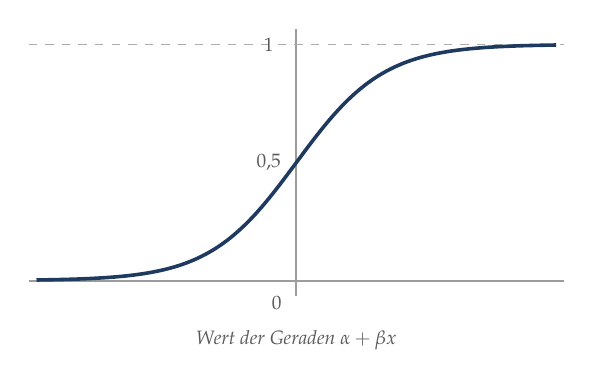
\begin{tikzpicture}[scale=1.0]
\draw[grau!60, line width=0.7pt] (-3.4,0) -- (3.4,0);
\draw[grau!60, line width=0.7pt] (0,-0.2) -- (0,3.2);
\draw[grau!50, dashed, line width=0.6pt] (-3.4,3.0) -- (3.4,3.0);
\draw[tief, line width=1.3pt, smooth, samples=80, domain=-3.3:3.3]
  plot (\x, {3.0/(1+exp(-1.8*\x))});
\node[font=\scriptsize, color=grau] at (-0.35,3.0) {$1$};
\node[font=\scriptsize, color=grau] at (-0.35,1.5) {$0{,}5$};
\node[font=\scriptsize, color=grau] at (-0.25,-0.28) {$0$};
\node[font=\scriptsize\itshape, color=grau] at (0,-0.75) {Wert der Geraden $\alpha + \beta x$};
\end{tikzpicture}
\end{center}

Die Kurve ist $S$-förmig, bleibt stets zwischen null und eins und ist in der Mitte am steilsten. Das entspricht der Anschauung: In der Nähe von $0{,}5$ bewirkt eine kleine Änderung der erklärenden Größe viel, an den Rändern wenig.
\end{merksatz}

\begin{merksatz}
\boxtitel{Die Deutung der Koeffizienten}
\begin{center}
\begin{minipage}{0.9\textwidth}
\textbf{$e^{\beta}$ ist das Chancenverhältnis je Einheit von $x$ --- bei festgehaltenen übrigen Größen.}
\end{minipage}
\end{center}

\schritt{Warum}
Erhöht man $x_1$ um eins, so wächst die linke Seite um $\beta_1$:
\[ \ln(\mathrm{odds}_{\text{neu}}) - \ln(\mathrm{odds}_{\text{alt}}) = \beta_1 \]
\[ \ln\frac{\mathrm{odds}_{\text{neu}}}{\mathrm{odds}_{\text{alt}}} = \beta_1 \quad\Longrightarrow\quad \frac{\mathrm{odds}_{\text{neu}}}{\mathrm{odds}_{\text{alt}}} = e^{\beta_1} . \]

\begin{center}
\renewcommand{\arraystretch}{1.45}
\begin{tabular}{@{}P{2.0cm}P{2.2cm}P{3.4cm}@{}}
\toprule
$\beta$ & $e^{\beta}$ & \\
\midrule
$0$ & $1{,}00$ & kein Zusammenhang\\
$0{,}69$ & $2{,}00$ & Chance verdoppelt\\
$-0{,}69$ & $0{,}50$ & Chance halbiert\\
$1{,}10$ & $3{,}00$ & \\
\bottomrule
\end{tabular}
\end{center}
\end{merksatz}

\begin{merksatz}
\boxtitel{Die MOBIL-Daten}
Bedarf an zusätzlichen Schmerzmitteln:
\begin{center}
\renewcommand{\arraystretch}{1.48}
\begin{tabular}{@{}P{1.8cm}P{1.6cm}P{1.6cm}P{1.6cm}@{}}
\toprule
& \textbf{ja} & \textbf{nein} & \textbf{Summe}\\
\midrule
A & $27$ & $33$ & $60$\\
B & $15$ & $45$ & $60$\\
\bottomrule
\end{tabular}
\end{center}

\schritt{Schritt 1 --- Die Chancen}
\[ \mathrm{odds}_A = \frac{27}{33} = 0{,}8182, \qquad \mathrm{odds}_B = \frac{15}{45} = 0{,}3333 \]

\schritt{Schritt 2 --- Das Chancenverhältnis}
\[ \mathrm{OR} = \frac{0{,}8182}{0{,}3333} = 2{,}455 \]

Die Kreuzproduktformel liefert dasselbe:
\[ \mathrm{OR} = \frac{27 \cdot 45}{33 \cdot 15} = \frac{1215}{495} = 2{,}4545 . \quad \checkmark \]

\schritt{Schritt 3 --- Das Konfidenzintervall}
Man rechnet auf der logarithmischen Skala, weil die Verteilung dort annähernd symmetrisch ist.
\[ \ln \mathrm{OR} = \ln 2{,}4545 = 0{,}8979 \]
\[ \widehat{\mathrm{SE}} = \sqrt{\frac{1}{27}+\frac{1}{33}+\frac{1}{15}+\frac{1}{45}} = \sqrt{0{,}03704+0{,}03030+0{,}06667+0{,}02222} \]
\[ = \sqrt{0{,}15623} = 0{,}3953 \]
\[ 0{,}8979 \pm 1{,}96 \cdot 0{,}3953 = 0{,}8979 \pm 0{,}7747 \quad\Longrightarrow\quad [\,0{,}1232\ ;\ 1{,}6726\,] \]

\schritt{Schritt 4 --- Zurückrechnen}
\[ e^{0{,}1232} = 1{,}131, \qquad e^{1{,}6726} = 5{,}327 \]
\[ \mathrm{OR} = 2{,}45 \quad (95\,\%\text{-KI } 1{,}13 \text{ bis } 5{,}33) \]

\schritt{Die Deutung}
Die Chance auf zusätzlichen Schmerzmittelbedarf ist unter dem bisherigen Schema etwa zweieinhalbmal so groß. Das Intervall schließt die Eins nicht ein --- gleichbedeutend mit $p < 0{,}05$.

\begin{center}
\begin{minipage}{0.88\textwidth}
\kursiv{Beachten Sie die Asymmetrie des Intervalls: von $1{,}13$ bis $5{,}33$, mit dem Schätzer bei $2{,}45$. Auf der logarithmischen Skala ist es symmetrisch; zurückgerechnet ist es das nicht. Das ist richtig so --- Chancenverhältnisse sind multiplikative Größen.}
\end{minipage}
\end{center}
\end{merksatz}

\begin{warnung}
\boxtitelr{Chancenverhältnis ist nicht Risikoverhältnis}
Dies ist die häufigste Fehldeutung der medizinischen Statistik.

\begin{center}
\renewcommand{\arraystretch}{1.5}
\begin{tabular}{@{}P{3.2cm}P{5.4cm}@{}}
\toprule
\textbf{Risiko\-verhältnis} & $\mathrm{RR} = \dfrac{\pi_A}{\pi_B}$ --- das Verhältnis der Wahrscheinlichkeiten\\[6pt]
\textbf{Chancen\-verhältnis} & $\mathrm{OR} = \dfrac{\pi_A/(1-\pi_A)}{\pi_B/(1-\pi_B)}$\\
\bottomrule
\end{tabular}
\end{center}

\schritt{Im Beispiel}
\[ \mathrm{RR} = \frac{0{,}45}{0{,}25} = 1{,}80 \qquad \text{gegen} \qquad \mathrm{OR} = 2{,}45 \]

Das Chancenverhältnis übertreibt den Effekt um mehr als ein Drittel.

\schritt{Wann der Unterschied klein ist}
\begin{center}
{\small
\renewcommand{\arraystretch}{1.45}
\begin{tabular}{@{}P{1.4cm}P{1.4cm}P{1.4cm}P{1.4cm}P{1.8cm}@{}}
\toprule
$\pi_B$ & $\pi_A$ & $\mathrm{RR}$ & $\mathrm{OR}$ & \textbf{Abwei\-chung}\\
\midrule
$0{,}01$ & $0{,}02$ & $2{,}00$ & $2{,}02$ & \textcolor{gruen}{$1\,\%$}\\
$0{,}10$ & $0{,}20$ & $2{,}00$ & $2{,}25$ & $13\,\%$\\
$0{,}25$ & $0{,}45$ & $1{,}80$ & $2{,}45$ & $36\,\%$\\
$0{,}40$ & $0{,}80$ & $2{,}00$ & $6{,}00$ & \textcolor{akzent}{$200\,\%$}\\
\bottomrule
\end{tabular}}
\end{center}

\begin{center}
\begin{minipage}{0.9\textwidth}
\textbf{Bei seltenen Ereignissen sind beide fast gleich. Bei häufigen übertreibt das Chancenverhältnis erheblich.}
\end{minipage}
\end{center}

\schritt{Warum man es trotzdem benutzt}
\begin{center}
\renewcommand{\arraystretch}{1.5}
\begin{tabular}{@{}P{2.6cm}P{6.0cm}@{}}
\toprule
\textbf{Fall-Kontroll-Studien} & Dort lässt sich das Risiko nicht schätzen, das Chancenverhältnis schon. Kapitel~12 erklärt warum.\\
\textbf{Rechenbarkeit} & Es fällt unmittelbar aus dem logistischen Modell.\\
\textbf{Symmetrie} & Es ändert sich nicht, wenn man Ereignis und Nichtereignis vertauscht.\\
\bottomrule
\end{tabular}
\end{center}

\begin{center}
\begin{minipage}{0.88\textwidth}
\kursiv{Die Empfehlung lautet: Bei häufigen Ereignissen zusätzlich das Risikoverhältnis oder die absolute Differenz angeben. Ein Chancenverhältnis von $2{,}45$ klingt nach mehr als \enquote{$45$ statt $25$ Prozent} --- und Letzteres ist die Zahl, die eine Entscheidung trägt.}
\end{minipage}
\end{center}
\end{warnung}

\section{Zeit bis zu einem Ereignis}

\begin{merksatz}
\boxtitel{Was hier anders ist}
Die Mobilisationszeit ist eine Zeitdauer. Bei manchen Personen weiß man sie nicht --- weil die Beobachtung endete, bevor das Ereignis eintrat.

\begin{center}
\renewcommand{\arraystretch}{1.5}
\begin{tabular}{@{}P{2.6cm}P{6.0cm}@{}}
\toprule
\textbf{Verlegung} & Die Person wurde nach $19$ Stunden in eine andere Klinik verlegt, noch nicht mobilisiert.\\
\textbf{Studienende} & Die Beobachtung endete, bevor das Ereignis eintrat.\\
\textbf{Abbruch} & Die Person zog die Einwilligung zurück.\\
\bottomrule
\end{tabular}
\end{center}

\begin{center}
\begin{minipage}{0.9\textwidth}
In allen drei Fällen weiß man: \textbf{Die wahre Zeit ist \kursiv{größer} als die beobachtete.} Man nennt solche Beobachtungen \Begriff{zensiert}.
\end{minipage}
\end{center}
\end{merksatz}

\begin{warnung}
\boxtitelr{Zwei naheliegende Behandlungen, beide falsch}
\begin{center}
\renewcommand{\arraystretch}{1.5}
\begin{tabular}{@{}P{2.6cm}P{6.0cm}@{}}
\toprule
\textbf{Weglassen} & Man wirft die zensierten Fälle weg. Das verzerrt: Gerade die langsamen Fälle werden bevorzugt zensiert, das Ergebnis wird zu günstig.\\
\textbf{Als Ereignis zählen} & Man behandelt $19^+$ wie $19$. Das unterschätzt die Zeit systematisch.\\
\bottomrule
\end{tabular}
\end{center}

\begin{center}
\begin{minipage}{0.88\textwidth}
\kursiv{Die zensierte Beobachtung enthält Auskunft --- nämlich dass die Person die ersten $19$ Stunden ohne Ereignis überstanden hat. Diese Auskunft will man nutzen, ohne etwas zu erfinden. Genau das leistet das Verfahren von Kaplan und Meier.}
\end{minipage}
\end{center}

\schritt{Die stillschweigende Voraussetzung}
\begin{center}
\begin{minipage}{0.9\textwidth}
\textbf{Zensierung muss \kursiv{uninformativ} sein:} Der Grund für das Ausscheiden darf nichts mit der Zielgröße zu tun haben.
\end{minipage}
\end{center}

Wird jemand verlegt, \kursiv{weil} es ihm schlecht geht, so ist diese Voraussetzung verletzt --- und kein Verfahren repariert das. Die Annahme ist nicht aus den Daten prüfbar.
\end{warnung}

\begin{merksatz}
\boxtitel{Der Schätzer von Kaplan und Meier}
\schritt{Der Grundgedanke}
Man zerlegt das Überstehen einer langen Zeit in viele kleine Schritte:
\[ S(t) = \Pr[\text{Ereignis tritt nach } t \text{ ein}] = \prod_{t_j \le t}\left(1 - \frac{d_j}{n_j}\right) \]
mit
\begin{center}
\renewcommand{\arraystretch}{1.45}
\begin{tabular}{@{}P{1.4cm}P{6.8cm}@{}}
\toprule
$t_j$ & Zeitpunkte, zu denen Ereignisse eintraten\\
$d_j$ & Anzahl der Ereignisse zu diesem Zeitpunkt\\
$n_j$ & Anzahl der \kursiv{Risikopersonen} unmittelbar davor\\
\bottomrule
\end{tabular}
\end{center}

\schritt{Warum ein Produkt}
Um $t$ zu überstehen, muss man jeden einzelnen Zeitpunkt davor überstanden haben. Die Wahrscheinlichkeiten multiplizieren sich --- wie bei einer Kette von Bedingungen.

\schritt{Was mit den Zensierten geschieht}
Sie zählen zum Nenner $n_j$, solange sie beobachtet werden, und scheiden danach still aus. Sie erscheinen nie im Zähler $d_j$.
\end{merksatz}

\begin{merksatz}
\boxtitel{Ein vollständiges Beispiel}
Zehn Personen der Gruppe A, Zeit bis zur Mobilisation in Stunden. Ein Pluszeichen bedeutet zensiert:
\[ 15,\quad 18,\quad 19^{+},\quad 21,\quad 24,\quad 26^{+},\quad 28,\quad 31,\quad 33^{+},\quad 35 \]

\schritt{Die Tabelle}
\begin{center}
{\small
\renewcommand{\arraystretch}{1.4}
\begin{tabular}{@{}P{1.2cm}P{1.4cm}P{1.2cm}P{2.4cm}P{1.8cm}@{}}
\toprule
$t_j$ & $n_j$ & $d_j$ & $1 - d_j/n_j$ & $S(t_j)$\\
\midrule
$15$ & $10$ & $1$ & $9/10 = 0{,}900$ & $0{,}900$\\
$18$ & $9$ & $1$ & $8/9 = 0{,}889$ & $0{,}800$\\
$19$ & $8$ & $0$ & \textcolor{grau}{zensiert} & $0{,}800$\\
$21$ & $7$ & $1$ & $6/7 = 0{,}857$ & $0{,}686$\\
$24$ & $6$ & $1$ & $5/6 = 0{,}833$ & $0{,}571$\\
$26$ & $5$ & $0$ & \textcolor{grau}{zensiert} & $0{,}571$\\
$28$ & $4$ & $1$ & $3/4 = 0{,}750$ & $\mathbf{0{,}429}$\\
$31$ & $3$ & $1$ & $2/3 = 0{,}667$ & $0{,}286$\\
$33$ & $2$ & $0$ & \textcolor{grau}{zensiert} & $0{,}286$\\
$35$ & $1$ & $1$ & $0/1 = 0$ & $0{,}000$\\
\bottomrule
\end{tabular}}
\end{center}

\schritt{Die Rechnung für $t = 24$, ausgeschrieben}
\[ S(24) = \frac{9}{10}\cdot\frac{8}{9}\cdot\frac{6}{7}\cdot\frac{5}{6} = 0{,}900 \cdot 0{,}889 \cdot 0{,}857 \cdot 0{,}833 = 0{,}571 \]

\schritt{Die Kurve}
\begin{center}
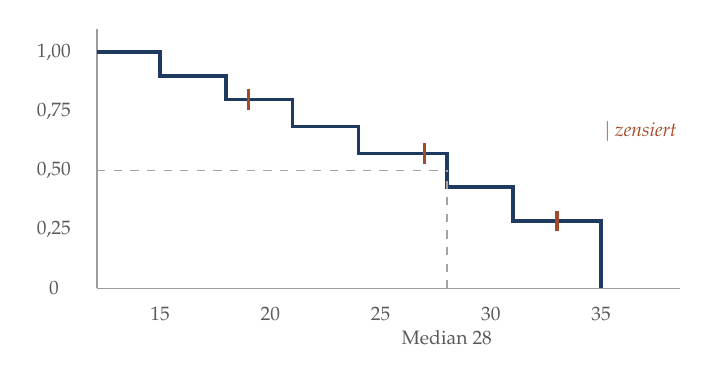
\begin{tikzpicture}[scale=1.0]
\draw[grau!60, line width=0.7pt] (0,0) -- (7.4,0);
\draw[grau!60, line width=0.7pt] (0,0) -- (0,3.3);
\foreach \y/\lab in {0/0, 0.75/{0{,}25}, 1.5/{0{,}50}, 2.25/{0{,}75}, 3.0/{1{,}00}}
  \node[font=\scriptsize, color=grau] at (-0.55,\y) {\lab};
\foreach \x/\lab in {0.8/15, 2.2/20, 3.6/25, 5.0/30, 6.4/35}
  \node[font=\scriptsize, color=grau] at (\x,-0.32) {\lab};
\draw[tief, line width=1.3pt]
 (0,3.0) -- (0.8,3.0) -- (0.8,2.7) -- (1.64,2.7) -- (1.64,2.4) --
 (2.48,2.4) -- (2.48,2.057) -- (3.32,2.057) -- (3.32,1.714) --
 (4.44,1.714) -- (4.44,1.286) -- (5.28,1.286) -- (5.28,0.857) --
 (6.4,0.857) -- (6.4,0);
\foreach \x/\y in {1.92/2.4, 4.16/1.714, 5.84/0.857} {
  \draw[akzent, line width=1.1pt] (\x,\y-0.13) -- (\x,\y+0.13);
}
\draw[grau!55, dashed, line width=0.6pt] (0,1.5) -- (4.44,1.5);
\draw[grau!55, dashed, line width=0.6pt] (4.44,0) -- (4.44,1.5);
\node[font=\scriptsize, color=grau] at (4.44,-0.62) {Median $28$};
\node[font=\scriptsize\itshape, color=akzent] at (6.9,2.0) {$|$ zensiert};
\end{tikzpicture}
\end{center}

\schritt{Die mediane Zeit ablesen}
Man sucht den ersten Zeitpunkt, an dem die Kurve auf $0{,}5$ oder darunter fällt: bei $t = 28$ Stunden.

\begin{center}
\begin{minipage}{0.88\textwidth}
\kursiv{Man berichtet den Median, nicht den Mittelwert. Der Grund: Endet die Beobachtung mit einer zensierten Person, so ist die Kurve nie bei null angelangt, und der Mittelwert ist gar nicht schätzbar. Der Median braucht nur, dass die Kurve unter $0{,}5$ fällt.}
\end{minipage}
\end{center}
\end{merksatz}

\begin{merksatz}
\boxtitel{Der Log-Rang-Test}
Zum Vergleich zweier Kurven benutzt man den \Begriff{Log-Rang-Test}. Sein Gedanke:

\begin{center}
\renewcommand{\arraystretch}{1.5}
\begin{tabular}{@{}P{1.0cm}P{7.4cm}@{}}
\toprule
$1$ & Zu jedem Ereigniszeitpunkt bildet man eine Vierfeldertafel: Gruppe gegen Ereignis.\\
$2$ & Unter $H_0$ berechnet man die erwartete Anzahl in jeder Gruppe --- wie beim $\chi^2$-Test.\\
$3$ & Man summiert beobachtete und erwartete Anzahlen über alle Zeitpunkte.\\
$4$ & Die Prüfgröße vergleicht beide Summen.\\
\bottomrule
\end{tabular}
\end{center}

\begin{center}
\begin{minipage}{0.88\textwidth}
\kursiv{Der Test nutzt die gesamte Kurve, nicht nur einen Zeitpunkt. Er ist am mächtigsten, wenn die Kurven sich nicht kreuzen. Kreuzen sie sich --- eine Therapie wirkt früh gut und spät schlecht ---, so kann er beides gegeneinander aufheben und nichts finden, obwohl ein deutlicher Unterschied besteht.}
\end{minipage}
\end{center}
\end{merksatz}

\section{Das Cox-Modell}

\begin{definition}
\boxtitelm{Definition 11.3 --- Hazard und Cox-Modell}
Die \Begriff{Hazardrate} $h(t)$ ist die momentane Ereignisrate zum Zeitpunkt $t$ --- gegeben, dass das Ereignis bis dahin nicht eingetreten ist.

Das \Begriff{Cox-Modell} lautet
\[ h(t \mid x) \;=\; h_0(t)\cdot e^{\beta_1x_1 + \cdots + \beta_kx_k} . \]
\end{definition}

\begin{merksatz}
\boxtitel{Warum dieses Modell so erfolgreich ist}
\begin{center}
\renewcommand{\arraystretch}{1.52}
\begin{tabular}{@{}P{2.6cm}P{6.0cm}@{}}
\toprule
\textbf{$h_0$ bleibt offen} & Über den zeitlichen Verlauf wird nichts angenommen. $h_0(t)$ darf jede Form haben.\\
\textbf{Nur das Verhältnis zählt} & Der Quotient zweier Hazardraten ist $e^{\beta}$ --- unabhängig von $t$, weil $h_0$ sich herauskürzt.\\
\textbf{Zensierung eingebaut} & Das Verfahren verarbeitet zensierte Beobachtungen wie Kaplan-Meier.\\
\bottomrule
\end{tabular}
\end{center}

\schritt{Die Deutung}
$e^{\beta}$ heißt \Begriff{Hazard Ratio}. Ein Wert von $0{,}6$ bedeutet: Die Ereignisrate ist zu jedem Zeitpunkt um $40\,\%$ niedriger.

\begin{center}
\begin{minipage}{0.88\textwidth}
\kursiv{\textbf{Nicht:} \enquote{Die Überlebenszeit ist um $40\,\%$ länger.} Das Verhältnis betrifft die Rate, nicht die Zeit. Die Umrechnung hängt von $h_0$ ab und ist selten einfach.}
\end{minipage}
\end{center}
\end{merksatz}

\begin{warnung}
\boxtitelr{Die Annahme proportionaler Hazards}
Der Name \enquote{proportional} steckt in der Formel: Das Verhältnis $e^\beta$ ist \kursiv{zeitunabhängig}. Trifft das nicht zu, so schätzt das Modell eine Art Durchschnitt über die Zeit, der irreführend sein kann.

\begin{center}
\renewcommand{\arraystretch}{1.5}
\begin{tabular}{@{}P{2.6cm}P{6.0cm}@{}}
\toprule
\textbf{Wann verletzt} & Wenn eine Behandlung früh wirkt und später nicht mehr --- oder umgekehrt.\\
\textbf{Wie prüfen} & Kurven der logarithmierten kumulierten Hazards auftragen; sie sollten parallel verlaufen. Oder ein Test auf zeitabhängige Koeffizienten.\\
\textbf{Was tun} & Zeitabhängige Koeffizienten, Aufteilung in Zeitabschnitte, oder ein anderes Modell.\\
\bottomrule
\end{tabular}
\end{center}

\begin{center}
\begin{minipage}{0.88\textwidth}
\kursiv{Diese Prüfung fehlt in einem erheblichen Teil der Veröffentlichungen, die Cox-Modelle berichten. Sie ist kein Zusatz, sondern die Voraussetzung dafür, dass die berichtete Zahl überhaupt etwas bedeutet.}
\end{minipage}
\end{center}
\end{warnung}

\section{Mehrebenenmodelle}

\begin{merksatz}
\boxtitel{Die Lösung für die Pseudoreplikation}
Kapitel~4 und 8 haben den Fall aufgeschoben: mehrere Messungen je Person, mehrere Personen je Zentrum.

\begin{center}
\begin{minipage}{0.9\textwidth}
Ein \Begriff{Mehrebenenmodell} erlaubt jeder Person --- oder jedem Zentrum --- einen eigenen Achsenabschnitt, der selbst als zufällig behandelt wird:
\[ y_{ij} = \alpha + u_i + \beta x_{ij} + \varepsilon_{ij} \]
\end{minipage}
\end{center}

\begin{center}
\renewcommand{\arraystretch}{1.5}
\begin{tabular}{@{}P{1.4cm}P{6.8cm}@{}}
\toprule
$u_i$ & Die Abweichung der $i$-ten Person vom Gesamtniveau --- zufällig, mit eigener Varianz.\\
$\varepsilon_{ij}$ & Die Abweichung der $j$-ten Messung an dieser Person.\\
\bottomrule
\end{tabular}
\end{center}

\schritt{Was das leistet}
Die Streuung wird in zwei Anteile zerlegt: zwischen den Personen und innerhalb. Der Standardfehler berücksichtigt, dass Messungen an derselben Person einander ähneln.

\begin{center}
\begin{minipage}{0.88\textwidth}
\kursiv{Und es leistet noch etwas: Die Schätzung für eine Person mit wenigen Messungen wird zum Gesamtmittel hin gezogen --- genau das Zusammenziehen aus Steins Befund in Kapitel~5. Mehrebenenmodelle sind die verbreitetste Anwendung dieses Prinzips.}
\end{minipage}
\end{center}
\end{merksatz}

\section{Übungsaufgaben}

\begin{aufgabe}
\boxtitel{Aufgabe 11.1 --- Chancenverhältnis und Risikoverhältnis}
In einer Studie trat eine Komplikation auf bei $40$ von $100$ Personen unter A und bei $20$ von $100$ unter B. Berechnen Sie beide Kennzahlen mit Intervall und beurteilen Sie den Unterschied.

\loesung
\schritt{Schritt 1 --- Die Risiken}
\[ \hat\pi_A = 0{,}40, \qquad \hat\pi_B = 0{,}20 \]

\schritt{Schritt 2 --- Das Risikoverhältnis}
\[ \mathrm{RR} = \frac{0{,}40}{0{,}20} = 2{,}00 \]
\[ \widehat{\mathrm{SE}}(\ln \mathrm{RR}) = \sqrt{\frac{1-\hat\pi_A}{100\,\hat\pi_A} + \frac{1-\hat\pi_B}{100\,\hat\pi_B}} = \sqrt{\frac{0{,}60}{40} + \frac{0{,}80}{20}} \]
\[ = \sqrt{0{,}015 + 0{,}040} = \sqrt{0{,}055} = 0{,}2345 \]
\[ \ln 2 = 0{,}6931; \qquad 0{,}6931 \pm 1{,}96 \cdot 0{,}2345 = 0{,}6931 \pm 0{,}4596 \]
\[ [\,e^{0{,}2335};\ e^{1{,}1527}\,] = [\,1{,}26\ ;\ 3{,}17\,] \]

\schritt{Schritt 3 --- Das Chancenverhältnis}
\[ \mathrm{OR} = \frac{40 \cdot 80}{60 \cdot 20} = \frac{3200}{1200} = 2{,}667 \]
\[ \widehat{\mathrm{SE}}(\ln \mathrm{OR}) = \sqrt{\frac{1}{40}+\frac{1}{60}+\frac{1}{20}+\frac{1}{80}} = \sqrt{0{,}025+0{,}01667+0{,}05+0{,}0125} \]
\[ = \sqrt{0{,}10417} = 0{,}3228 \]
\[ \ln 2{,}667 = 0{,}9808; \qquad 0{,}9808 \pm 1{,}96 \cdot 0{,}3228 = 0{,}9808 \pm 0{,}6327 \]
\[ [\,e^{0{,}3481};\ e^{1{,}6135}\,] = [\,1{,}42\ ;\ 5{,}02\,] \]

\schritt{Schritt 4 --- Die absolute Differenz}
\[ 0{,}40 - 0{,}20 = 0{,}20 \]
Das ist die Größe, die eine Entscheidung trägt: Von hundert Behandelten haben zwanzig mehr eine Komplikation.

\schritt{Schritt 5 --- Der Vergleich}
\begin{center}
\renewcommand{\arraystretch}{1.48}
\begin{tabular}{@{}P{3.2cm}P{1.6cm}P{2.6cm}@{}}
\toprule
\textbf{Kennzahl} & \textbf{Wert} & \textbf{$95\,\%$-KI}\\
\midrule
Risikodifferenz & $0{,}20$ & --- \\
Risiko\-verhältnis & $2{,}00$ & $[1{,}26;\ 3{,}17]$\\
Chancen\-verhältnis & $\mathbf{2{,}67}$ & $[1{,}42;\ 5{,}02]$\\
\bottomrule
\end{tabular}
\end{center}

Das Chancenverhältnis liegt um ein Drittel über dem Risikoverhältnis --- weil das Ereignis mit $20$ bis $40$ Prozent häufig ist.

\schritt{Die Empfehlung}
\begin{center}
\begin{minipage}{0.86\textwidth}
\kursiv{Man berichtet hier die Risikodifferenz und das Risikoverhältnis. Ein Chancenverhältnis von $2{,}67$ zu nennen, ohne die Häufigkeit anzugeben, wäre irreführend --- der Leser rechnet es gedanklich als Risikoverhältnis um.}
\end{minipage}
\end{center}
\end{aufgabe}

\begin{aufgabe}
\boxtitel{Aufgabe 11.2 --- Eine Kaplan-Meier-Kurve}
Acht Personen, Zeit bis zum Ereignis in Tagen:
\[ 3,\quad 5^{+},\quad 7,\quad 10,\quad 12^{+},\quad 15,\quad 18^{+},\quad 20 \]
Bestimmen Sie die Kurve und die mediane Zeit.

\loesung
\schritt{Schritt 1 --- Die Tabelle}
\begin{center}
{\small
\renewcommand{\arraystretch}{1.4}
\begin{tabular}{@{}P{1.2cm}P{1.2cm}P{1.2cm}P{2.2cm}P{1.8cm}@{}}
\toprule
$t_j$ & $n_j$ & $d_j$ & $1-d_j/n_j$ & $S(t_j)$\\
\midrule
$3$ & $8$ & $1$ & $7/8 = 0{,}875$ & $0{,}875$\\
$5$ & $7$ & $0$ & \textcolor{grau}{zensiert} & $0{,}875$\\
$7$ & $6$ & $1$ & $5/6 = 0{,}833$ & $0{,}729$\\
$10$ & $5$ & $1$ & $4/5 = 0{,}800$ & $\mathbf{0{,}583}$\\
$12$ & $4$ & $0$ & \textcolor{grau}{zensiert} & $0{,}583$\\
$15$ & $3$ & $1$ & $2/3 = 0{,}667$ & $\mathbf{0{,}389}$\\
$18$ & $2$ & $0$ & \textcolor{grau}{zensiert} & $0{,}389$\\
$20$ & $1$ & $1$ & $0/1 = 0$ & $0{,}000$\\
\bottomrule
\end{tabular}}
\end{center}

\schritt{Schritt 2 --- Die Rechnung nachvollziehen}
\[ S(10) = \frac{7}{8}\cdot\frac{5}{6}\cdot\frac{4}{5} = 0{,}875 \cdot 0{,}8333 \cdot 0{,}800 = 0{,}5833 \]
\[ S(15) = 0{,}5833 \cdot \frac{2}{3} = 0{,}3889 \]

\schritt{Schritt 3 --- Der Median}
Die Kurve fällt erstmals bei $t = 15$ unter $0{,}5$ --- von $0{,}583$ auf $0{,}389$.

\textbf{Mediane Zeit: $\mathbf{15}$ Tage.}

\schritt{Schritt 4 --- Die Probe: Wie viele Risikopersonen?}
Nach Ereignissen und Zensierungen abgezählt:
\begin{center}
{\small
\renewcommand{\arraystretch}{1.35}
\begin{tabular}{@{}P{1.2cm}P{2.4cm}P{2.4cm}@{}}
\toprule
$t$ & \textbf{ausgeschieden} & \textbf{verbleibend}\\
\midrule
$3$ & $1$ Ereignis & $7$\\
$5$ & $1$ zensiert & $6$\\
$7$ & $1$ Ereignis & $5$\\
$10$ & $1$ Ereignis & $4$\\
$12$ & $1$ zensiert & $3$\\
$15$ & $1$ Ereignis & $2$\\
$18$ & $1$ zensiert & $1$\\
$20$ & $1$ Ereignis & $0$\\
\bottomrule
\end{tabular}}
\end{center}
Die Spalte \enquote{verbleibend} stimmt mit den $n_j$ der nächsten Zeile überein. \checkmark

\schritt{Schritt 5 --- Ein naiver Vergleich}
Rechnete man die drei zensierten Fälle als Ereignisse, so wäre der Median der acht Werte $3,5,7,10,12,15,18,20$ gleich
\[ \frac{10+12}{2} = 11 \ \text{Tage} . \]
Also $11$ statt $15$ --- eine Unterschätzung um mehr als ein Viertel.

Ließe man sie weg, blieben $3, 7, 10, 15, 20$ mit Median $10$ --- noch schlechter.

\begin{center}
\begin{minipage}{0.86\textwidth}
\kursiv{Beide naiven Wege verkürzen die geschätzte Zeit. Bei fünf Ereignissen und drei Zensierungen ist der Unterschied erheblich; bei Studien mit überwiegend zensierten Beobachtungen --- etwa Langzeitüberleben --- wäre er dramatisch.}
\end{minipage}
\end{center}
\end{aufgabe}

\begin{aufgabe}
\boxtitel{Aufgabe 11.3 --- Ein logistisches Modell deuten}
Eine Auswertung liefert für das Auftreten einer Wundinfektion:
\begin{center}
{\small
\renewcommand{\arraystretch}{1.4}
\begin{tabular}{@{}P{3.0cm}P{1.6cm}P{1.6cm}P{2.0cm}@{}}
\toprule
\textbf{Größe} & $\beta$ & $e^{\beta}$ & \textbf{$95\,\%$-KI}\\
\midrule
Alter (je 10 Jahre) & $0{,}22$ & $1{,}25$ & $[1{,}08;\ 1{,}44]$\\
Diabetes (ja) & $0{,}69$ & $2{,}00$ & $[1{,}21;\ 3{,}31]$\\
OP-Dauer (je 30 min) & $0{,}41$ & $1{,}51$ & $[1{,}19;\ 1{,}91]$\\
Neues Schema & $-0{,}51$ & $0{,}60$ & $[0{,}38;\ 0{,}95]$\\
\bottomrule
\end{tabular}}
\end{center}
Deuten Sie die vier Zeilen und berechnen Sie die vorhergesagte Wahrscheinlichkeit für eine Person mit gegebenen Merkmalen, wenn $\alpha = -4{,}2$ ist.

\loesung
\schritt{Schritt 1 --- Die vier Zeilen}
\begin{center}
{\small
\renewcommand{\arraystretch}{1.5}
\begin{tabular}{@{}P{2.4cm}P{6.2cm}@{}}
\toprule
Alter & Je zehn Jahre steigt die Chance um $25\,\%$ --- bei gleichem Diabetesstatus, gleicher OP-Dauer, gleichem Schema.\\
Diabetes & Die Chance ist verdoppelt.\\
OP-Dauer & Je halbe Stunde steigt die Chance um $51\,\%$.\\
Neues Schema & Die Chance sinkt um $40\,\%$. Das Intervall reicht bis $0{,}95$ --- knapp unter eins.\\
\bottomrule
\end{tabular}}
\end{center}

\schritt{Schritt 2 --- Die Person}
Sagen wir: $70$ Jahre, Diabetes ja, OP-Dauer $90$ Minuten, neues Schema.

Die Größen sind je Einheit kodiert. Wir müssen festlegen, worauf sich $\alpha$ bezieht; nehmen wir an, Alter zählt in Jahrzehnten ab null und OP-Dauer in Halbstunden ab null.
\[ \text{Alter} = 7{,}0, \quad \text{Diabetes} = 1, \quad \text{OP-Dauer} = 3{,}0, \quad \text{Schema} = 1 \]

\schritt{Schritt 3 --- Den Logit ausrechnen}
\begin{align*}
\operatorname{logit} &= -4{,}2 + 0{,}22 \cdot 7{,}0 + 0{,}69 \cdot 1 + 0{,}41 \cdot 3{,}0 + (-0{,}51)\cdot 1\\
&= -4{,}2 + 1{,}54 + 0{,}69 + 1{,}23 - 0{,}51\\
&= -1{,}25
\end{align*}

\schritt{Schritt 4 --- Zurückrechnen}
\[ \pi = \frac{1}{1+e^{1{,}25}} = \frac{1}{1+3{,}490} = \frac{1}{4{,}490} = 0{,}223 \]

\textbf{Etwa $22\,\%$.}

\schritt{Schritt 5 --- Die Kontrollrechnung über die Chance}
\[ \mathrm{odds} = e^{-1{,}25} = 0{,}2865 \]
\[ \pi = \frac{0{,}2865}{1+0{,}2865} = \frac{0{,}2865}{1{,}2865} = 0{,}2227 . \quad \checkmark \]

\schritt{Schritt 6 --- Was dieselbe Person unter dem alten Schema hätte}
\[ \operatorname{logit} = -1{,}25 + 0{,}51 = -0{,}74 \]
\[ \pi = \frac{1}{1+e^{0{,}74}} = \frac{1}{1+2{,}096} = 0{,}323 \]

\begin{center}
\renewcommand{\arraystretch}{1.48}
\begin{tabular}{@{}P{2.8cm}P{2.0cm}P{2.6cm}@{}}
\toprule
& $\pi$ & \\
\midrule
Altes Schema & $0{,}323$ & \\
Neues Schema & $0{,}223$ & \\
\midrule
Differenz & $\mathbf{0{,}100}$ & $10$ von $100$\\
\bottomrule
\end{tabular}
\end{center}

\schritt{Die Lehre}
Das Chancenverhältnis $0{,}60$ ist für alle Personen dasselbe. Die \kursiv{absolute} Wirkung ist es nicht: Bei einer Person mit geringem Grundrisiko --- etwa $5\,\%$ --- sänke es nur auf $3{,}1\,\%$, also um $1{,}9$ Punkte statt um $10$.

\begin{center}
\begin{minipage}{0.86\textwidth}
\kursiv{Deshalb ist die absolute Risikodifferenz personenbezogen und das Chancenverhältnis nicht. Für die Frage \enquote{lohnt sich das für diesen Menschen?} braucht man beides --- das Modell und das Grundrisiko.}
\end{minipage}
\end{center}
\end{aufgabe}

\begin{geschichte}
\boxtitelg{Zwei Arbeiten, die das Fach verändert haben}
\Person{Edward Kaplan} und \Person{Paul Meier} reichten 1958 unabhängig voneinander fast dieselbe Arbeit beim selben Herausgeber ein. Dieser überzeugte beide, gemeinsam zu veröffentlichen. Die Verhandlungen dauerten vier Jahre; die Arbeit erschien schließlich im \kursiv{Journal of the American Statistical Association} und ist heute eine der meistzitierten Arbeiten der Statistik überhaupt.

\begin{center}
\begin{minipage}{0.9\textwidth}
\kursiv{Paul Meier wurde später auch als entschiedener Verfechter der Randomisierung bekannt. Er setzte sich in den 1970er Jahren gegen erheblichen Widerstand dafür ein, dass klinische Studien randomisiert werden --- ein Kampf, den Kapitel~12 aufgreift.}
\end{minipage}
\end{center}

\Person{David Cox} veröffentlichte 1972 das nach ihm benannte Modell. Der Kunstgriff --- die Grundrate $h_0(t)$ unbestimmt zu lassen und nur das Verhältnis zu schätzen --- war so ungewöhnlich, dass in der Diskussion zur Arbeit mehrere angesehene Statistiker bezweifelten, dass das überhaupt zulässig sei.

Cox lieferte die theoretische Rechtfertigung zwei Jahre später nach, mit dem Begriff der \Begriff{partiellen Likelihood}. Sein Aufsatz von 1972 ist die meistzitierte Arbeit der gesamten Statistik.
\end{geschichte}

\begin{forschung}
\boxtitelp{Was an diesen Modellen heute diskutiert wird}
\begin{center}
{\small
\renewcommand{\arraystretch}{1.45}
\begin{tabular}{@{}P{3.0cm}P{5.2cm}@{}}
\toprule
\textbf{Weg vom Chancen\-verhältnis} & Bei häufigen Ereignissen setzen sich Modelle durch, die unmittelbar das Risikoverhältnis oder die Risikodifferenz schätzen.\\
\textbf{Konkurrierende Ereignisse} & Stirbt jemand an anderer Ursache, ist das keine gewöhnliche Zensierung. Kaplan-Meier überschätzt dann das Risiko; man braucht die kumulierte Inzidenzfunktion.\\
\textbf{Nichtpro\-portionale Hazards} & In der Immuntherapie kreuzen sich Kurven regelmäßig. Es gibt Vorschläge für Ersatzmaße, etwa die eingeschränkte mittlere Überlebenszeit.\\
\bottomrule
\end{tabular}}
\end{center}

Die zweite Zeile ist eine verbreitete Fehlerquelle. Wer die Zeit bis zum Rückfall untersucht und Todesfälle anderer Ursache als zensiert behandelt, nimmt stillschweigend an, diese Personen hätten dasselbe Rückfallrisiko gehabt wie die übrigen. Bei älteren oder schwer kranken Personen trifft das nicht zu.

\begin{center}
\begin{minipage}{0.88\textwidth}
\kursiv{Die dritte Zeile betrifft ein wachsendes Feld: Bei Immuntherapien wirkt die Behandlung oft erst nach Monaten, dafür dann dauerhaft. Die Kurven liegen anfangs übereinander und trennen sich spät --- die Annahme proportionaler Hazards ist klar verletzt, und das Hazard Ratio mittelt über zwei völlig verschiedene Abschnitte.}
\end{minipage}
\end{center}
\end{forschung}

\begin{merksatz}
\boxtitel{Was Sie jetzt können}
\begin{center}
\renewcommand{\arraystretch}{1.5}
\begin{tabular}{@{}P{3.0cm}P{5.6cm}@{}}
\toprule
\textbf{Logit} & warum man nicht die Wahrscheinlichkeit selbst modelliert\\
\textbf{$e^{\beta}$} & Chancenverhältnis --- und wann es das Risiko übertreibt\\
\textbf{Zensierung} & und warum Weglassen und Mitzählen beide falsch sind\\
\textbf{Kaplan-Meier} & vollständig von Hand gerechnet\\
\textbf{Cox} & Hazard Ratio und die Proportionalitätsannahme\\
\bottomrule
\end{tabular}
\end{center}

\begin{center}
\begin{minipage}{0.88\textwidth}
\kursiv{Damit endet Teil~IV. Ab Kapitel~12 geht es nicht mehr um Rechenverfahren, sondern um die Frage, wie man Daten erhebt, aus denen sich überhaupt etwas schließen lässt.}
\end{minipage}
\end{center}
\end{merksatz}

\part{Medizinische Statistik}

\chapter{Studiendesign}

\section{Die Frage vor allen Fragen}

\begin{merksatz}
\boxtitel{Ein Satz, der elf Kapitel zusammenfasst}
\begin{center}
\begin{minipage}{0.9\textwidth}
\textbf{Kein Rechenverfahren kann reparieren, was bei der Erhebung falsch gemacht wurde.}
\end{minipage}
\end{center}

\begin{center}
\renewcommand{\arraystretch}{1.5}
\begin{tabular}{@{}P{2.8cm}P{5.8cm}@{}}
\toprule
\textbf{Kapitel 3} & Korrelation unterscheidet die vier Erklärungen nicht.\\
\textbf{Kapitel 4} & Bei Abhängigkeit gilt kein Standardfehler.\\
\textbf{Kapitel 8} & Gegen verletzte Unabhängigkeit hilft kein Test.\\
\textbf{Kapitel 10} & Regression zur Mitte täuscht Wirkung vor.\\
\textbf{Kapitel 11} & Informative Zensierung verzerrt jede Kurve.\\
\bottomrule
\end{tabular}
\end{center}

\begin{center}
\begin{minipage}{0.88\textwidth}
\kursiv{In jedem dieser Fälle war die Abhilfe dieselbe: nicht anders rechnen, sondern anders erheben. Dieses Kapitel handelt davon.}
\end{minipage}
\end{center}
\end{merksatz}

\section{Die Ordnung der Studientypen}

\begin{merksatz}
\boxtitel{Von unten nach oben}
\begin{center}
{\small
\renewcommand{\arraystretch}{1.5}
\begin{tabular}{@{}P{2.8cm}P{3.0cm}P{2.4cm}@{}}
\toprule
\textbf{Typ} & \textbf{Beantwortet} & \textbf{Kausalität}\\
\midrule
Fallbericht & Was ist möglich? & \textcolor{akzent}{nein}\\
Ökologische Studie & Gruppenmuster & \textcolor{akzent}{nein}\\
Querschnitt & Wie häufig, jetzt? & \textcolor{akzent}{nein}\\
Fall-Kontroll & Rückblick auf Exposition & \textcolor{mittel}{schwach}\\
Kohorte & Vorwärts beobachtet & \textcolor{mittel}{mittel}\\
\textbf{Randomisiert} & \textbf{Wirkt es?} & \textcolor{gruen}{\textbf{ja}}\\
Metaanalyse & Alles zusammen & \textcolor{gruen}{so gut wie die Teile}\\
\bottomrule
\end{tabular}}
\end{center}

\begin{center}
\begin{minipage}{0.88\textwidth}
\kursiv{Die letzte Zeile steht bewusst nicht oben. Eine Metaanalyse ist nie besser als die Studien, die sie zusammenfasst --- Kapitel~14 geht darauf ein. Und der Sprung zwischen Zeile fünf und sechs ist der entscheidende: Erst dort wird die Zuteilung vom Zufall bestimmt statt von Menschen.}
\end{minipage}
\end{center}
\end{merksatz}

\begin{warnung}
\boxtitelr{Die Ordnung ist keine Rangliste der Wichtigkeit}
\begin{center}
\renewcommand{\arraystretch}{1.5}
\begin{tabular}{@{}P{2.8cm}P{5.8cm}@{}}
\toprule
\textbf{Seltene Ereignisse} & Eine Fall-Kontroll-Studie findet, was in einer randomisierten Studie nie aufträte.\\
\textbf{Schaden} & Man randomisiert niemanden auf eine vermutete Schädigung.\\
\textbf{Langzeitfolgen} & Über vierzig Jahre randomisiert niemand.\\
\textbf{Seltene Krankheiten} & Die nötige Fallzahl ist nicht erreichbar.\\
\bottomrule
\end{tabular}
\end{center}

\begin{center}
\begin{minipage}{0.88\textwidth}
\kursiv{Der Zusammenhang zwischen Rauchen und Lungenkrebs wurde nie randomisiert geprüft und ist trotzdem gesichert --- über die Kriterien am Ende dieses Kapitels. Die Ordnung sagt, wie leicht eine kausale Deutung fällt, nicht welche Frage wichtig ist.}
\end{minipage}
\end{center}
\end{warnung}

\section{Randomisierung}

\begin{merksatz}
\boxtitel{Was sie leistet --- drei Dinge}
\begin{center}
{\small
\renewcommand{\arraystretch}{1.55}
\begin{tabular}{@{}P{2.6cm}P{6.0cm}@{}}
\toprule
\textbf{Auch das Unbekannte} & Die Gruppen sind im Mittel gleich --- nicht nur in gemessenen Merkmalen, sondern in \kursiv{allen}. Auch in denen, an die niemand gedacht hat.\\
\textbf{Keine Auswahl} & Die Zuteilung hängt nicht davon ab, wen die Behandelnden für geeignet halten.\\
\textbf{Die Rechengrundlage} & Die Nullverteilung folgt aus dem Losverfahren --- Kapitel~9, Permutationstest.\\
\bottomrule
\end{tabular}}
\end{center}

\begin{center}
\begin{minipage}{0.9\textwidth}
\textbf{Die erste Zeile ist die entscheidende und wird oft unterschätzt.} Für gemessene Störgrößen kann man rechnerisch adjustieren (Kapitel~10). Für ungemessene kann man das nicht --- und man weiß nicht einmal, welche es gibt. Nur die Randomisierung gleicht sie aus.
\end{minipage}
\end{center}
\end{merksatz}

\begin{warnung}
\boxtitelr{Was sie nicht leistet}
\begin{center}
\renewcommand{\arraystretch}{1.5}
\begin{tabular}{@{}P{3.0cm}P{5.6cm}@{}}
\toprule
\textbf{Gleichheit im Einzelfall} & Die Gruppen sind \kursiv{im Mittel} gleich, nicht in jeder einzelnen Studie. Zufällige Ungleichheiten kommen vor.\\
\textbf{Übertrag\-barkeit} & Die Personen der Studie sind nicht zufällig aus der Bevölkerung gezogen. Die Wirkung gilt für sie, nicht ohne Weiteres für andere.\\
\textbf{Schutz vor allem Weiteren} & Verblindung, Nachbeobachtung, Auswertung können weiterhin schiefgehen.\\
\bottomrule
\end{tabular}
\end{center}

\schritt{Zur zweiten Zeile --- eine wichtige Unterscheidung}
\begin{center}
{\small
\renewcommand{\arraystretch}{1.5}
\begin{tabular}{@{}P{2.6cm}P{2.4cm}P{3.0cm}@{}}
\toprule
& \textbf{zufällig?} & \textbf{sichert}\\
\midrule
Auswahl der Personen & \textcolor{akzent}{meist nein} & äußere Gültigkeit\\
Zuteilung auf Gruppen & \textcolor{gruen}{ja} & innere Gültigkeit\\
\bottomrule
\end{tabular}}
\end{center}

\begin{center}
\begin{minipage}{0.88\textwidth}
\kursiv{Die MOBIL-Studie randomisiert die Zuteilung, nicht die Auswahl --- das war die offene Frage aus Kapitel~4. Damit ist der \kursiv{Vergleich} der beiden Gruppen gültig. Ob das Ergebnis auf andere Kliniken übertragbar ist, folgt daraus nicht und ist eine Frage des Fachurteils.}
\end{minipage}
\end{center}
\end{warnung}

\begin{merksatz}
\boxtitel{Wie man randomisiert}
\begin{center}
{\small
\renewcommand{\arraystretch}{1.5}
\begin{tabular}{@{}P{2.4cm}P{3.0cm}P{2.6cm}@{}}
\toprule
\textbf{Verfahren} & \textbf{Vorgehen} & \textbf{Eignung}\\
\midrule
Einfach & Münzwurf je Person & \textcolor{mittel}{ungleiche Gruppen möglich}\\
Blockweise & Blöcke fester Größe, darin ausgeglichen & \textcolor{gruen}{Standard}\\
Geschichtet & getrennt je Zentrum, Altersgruppe & \textcolor{gruen}{bei wichtigen Störgrößen}\\
Minimierung & jeweils zur Gruppe mit dem größeren Bedarf & bei kleinen Studien\\
\bottomrule
\end{tabular}}
\end{center}

\schritt{Warum nicht abwechselnd}
Ein Verfahren wie \enquote{abwechselnd A und B} oder \enquote{gerade Geburtstage nach A} ist \kursiv{nicht} zufällig, weil es \Begriff{vorhersagbar} ist.

\begin{center}
\begin{minipage}{0.9\textwidth}
Wer weiß, welche Gruppe als Nächstes kommt, kann die Zuteilung beeinflussen --- indem er eine Person aufnimmt oder nicht, sie früher oder später einschließt.
\end{minipage}
\end{center}

\schritt{Verdeckte Zuteilung}
Deshalb gehört zur Randomisierung die \Begriff{verdeckte Zuteilung}: Die Zuordnung ist bis zum Einschluss unbekannt --- durch eine zentrale Stelle, ein Rechnerverfahren oder nummerierte, undurchsichtige, versiegelte Umschläge.

\begin{center}
\begin{minipage}{0.88\textwidth}
\kursiv{Untersuchungen zeigen, dass Studien ohne verdeckte Zuteilung im Mittel um etwa dreißig Prozent größere Behandlungseffekte berichten. Das ist einer der am besten belegten Zusammenhänge der Methodenforschung.}
\end{minipage}
\end{center}
\end{merksatz}

\section{Verblindung}

\begin{merksatz}
\boxtitel{Wer was nicht wissen darf}
\begin{center}
{\small
\renewcommand{\arraystretch}{1.5}
\begin{tabular}{@{}P{2.6cm}P{6.0cm}@{}}
\toprule
\textbf{Die Person} & sonst wirken Erwartung und Berichtsverhalten auf das Ergebnis\\
\textbf{Die Behandelnden} & sonst unterscheidet sich die übrige Versorgung\\
\textbf{Die Erhebenden} & sonst wird der Endpunkt unterschiedlich gemessen\\
\textbf{Die Auswertenden} & sonst werden Entscheidungen in der Analyse beeinflusst\\
\bottomrule
\end{tabular}}
\end{center}

\begin{center}
\begin{minipage}{0.88\textwidth}
\kursiv{Die Bezeichnungen \enquote{einfach} und \enquote{doppelt blind} sind uneinheitlich --- verschiedene Veröffentlichungen meinen Verschiedenes. Die CONSORT-Empfehlungen verlangen deshalb, ausdrücklich aufzuzählen, wer verblindet war.}
\end{minipage}
\end{center}

\schritt{Wann Verblindung besonders wichtig ist}
\begin{center}
\renewcommand{\arraystretch}{1.48}
\begin{tabular}{@{}P{3.0cm}P{2.4cm}P{2.4cm}@{}}
\toprule
\textbf{Endpunkt} & \textbf{Beein\-flussbar?} & \\
\midrule
Tod & \textcolor{gruen}{kaum} & robust\\
Laborwert & \textcolor{gruen}{wenig} & ziemlich robust\\
Schmerzangabe & \textcolor{akzent}{\textbf{stark}} & \textcolor{akzent}{Verblindung nötig}\\
Zeitpunkt der Mobilisation & \textcolor{akzent}{\textbf{stark}} & wer entscheidet darüber?\\
\bottomrule
\end{tabular}
\end{center}

\begin{center}
\begin{minipage}{0.88\textwidth}
\kursiv{Die letzte Zeile betrifft die MOBIL-Studie unmittelbar: Wenn die Pflegekraft weiß, welches Schema die Person bekam, und sie zum Aufstehen ermutigt, so misst die Studie auch diese Ermutigung. Ein Endpunkt, über den Menschen mit Kenntnis der Gruppe entscheiden, ist nur bei Verblindung belastbar.}
\end{minipage}
\end{center}
\end{merksatz}

\section{Der Bias-Katalog}

\begin{merksatz}
\boxtitel{Die wichtigsten systematischen Fehler}
\begin{center}
{\small
\renewcommand{\arraystretch}{1.5}
\begin{tabular}{@{}P{2.4cm}P{3.0cm}P{2.6cm}@{}}
\toprule
\textbf{Name} & \textbf{Was geschieht} & \textbf{Abhilfe}\\
\midrule
Auswahl & Gruppen anders zusammen\-gesetzt & Randomisierung\\
Zuteilung & Zuordnung beeinflusst & verdeckte Zuteilung\\
Durchführung & übrige Versorgung ungleich & Verblindung\\
Messung & Endpunkt ungleich erhoben & verblindete Erhebung\\
\textbf{Ausfall} & Ausgeschiedene unterscheiden sich & \textcolor{akzent}{\textbf{schwer}}\\
Berichts & nur günstige Endpunkte berichtet & Prä\-registrierung\\
Publikations & nur positive Studien erscheinen & Register\\
\bottomrule
\end{tabular}}
\end{center}

\schritt{Warum der Ausfall so schwer zu beheben ist}
Er tritt nach der Randomisierung ein. Alles, was die Randomisierung gesichert hat, kann durch ungleiches Ausscheiden wieder zerstört werden.

\begin{center}
\begin{minipage}{0.88\textwidth}
\kursiv{Als Faustregel gilt: Bis etwa fünf Prozent Ausfall ist das Ergebnis kaum betroffen, ab zwanzig Prozent wird es fragwürdig. Entscheidend ist aber nicht die Zahl, sondern ob sich die Ausgeschiedenen von den Verbliebenen unterscheiden --- und das lässt sich nur vermuten.}
\end{minipage}
\end{center}
\end{merksatz}

\begin{warnung}
\boxtitelr{Zwei Verzerrungen, die man leicht übersieht}
\schritt{Der unsterbliche Zeitraum}
Vergleicht man Personen, die eine Behandlung erhielten, mit solchen, die sie nicht erhielten, so mussten die Ersten lange genug leben, um sie zu bekommen.

\begin{center}
\begin{minipage}{0.88\textwidth}
\kursiv{Ein bekanntes Beispiel: Empfänger einer Transplantation überleben länger als Personen auf der Warteliste. Ein Teil davon ist der Vorteil der Transplantation --- ein Teil ist der Umstand, dass man sie nur bekommt, wenn man bis dahin überlebt hat.}
\end{minipage}
\end{center}

\schritt{Die Vorlaufzeit}
Eine Früherkennung verlängert die Zeit \kursiv{ab Diagnose} auch dann, wenn sie den Todeszeitpunkt nicht verschiebt --- sie verlegt nur die Diagnose nach vorn.

\begin{center}
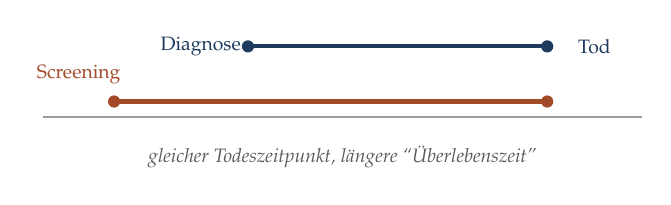
\begin{tikzpicture}[scale=1.0]
\draw[grau!60, line width=0.7pt] (0,0) -- (7.6,0);
\draw[tief, line width=1.5pt] (2.6,0.9) -- (6.4,0.9);
\fill[tief] (2.6,0.9) circle (2.2pt); \fill[tief] (6.4,0.9) circle (2.2pt);
\node[font=\scriptsize, color=tief] at (2.0,0.9) {Diagnose};
\node[font=\scriptsize, color=tief] at (7.0,0.9) {Tod};
\draw[akzent, line width=1.5pt] (0.9,0.2) -- (6.4,0.2);
\fill[akzent] (0.9,0.2) circle (2.2pt); \fill[akzent] (6.4,0.2) circle (2.2pt);
\node[font=\scriptsize, color=akzent] at (0.45,0.55) {Screening};
\node[font=\scriptsize\itshape, color=grau] at (3.8,-0.5) {gleicher Todeszeitpunkt, längere \enquote{Überlebenszeit}};
\end{tikzpicture}
\end{center}

\begin{center}
\begin{minipage}{0.88\textwidth}
\kursiv{Deshalb ist die Fünfjahresüberlebensrate kein taugliches Maß für den Nutzen einer Früherkennung. Das taugliche Maß ist die \kursiv{Sterblichkeit} in der gesamten eingeladenen Bevölkerung --- und die sinkt bei vielen Screeningprogrammen deutlich weniger, als die Überlebensraten nahelegen.}
\end{minipage}
\end{center}
\end{warnung}

\section{Kohorte und Fall-Kontroll-Studie}

\begin{merksatz}
\boxtitel{Die zwei Blickrichtungen}
\begin{center}
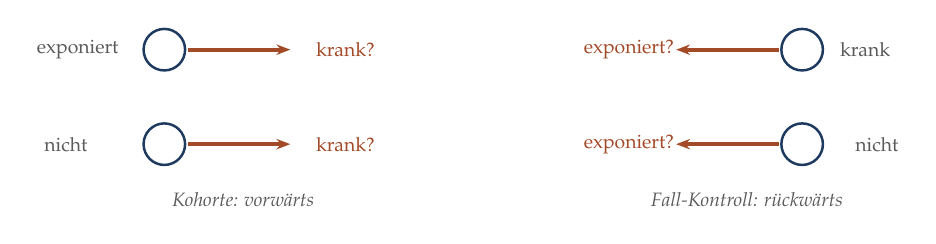
\begin{tikzpicture}[scale=1.0]
\begin{scope}
\node[knotenb] (e) at (0,0.6) {};
\node[knotenb] (ne) at (0,-0.6) {};
\node[font=\scriptsize, color=grau] at (-1.1,0.6) {exponiert};
\node[font=\scriptsize, color=grau] at (-1.25,-0.6) {nicht};
\draw[kanted, -{Stealth[length=5pt]}] (0.3,0.6) -- (1.6,0.6);
\draw[kanted, -{Stealth[length=5pt]}] (0.3,-0.6) -- (1.6,-0.6);
\node[font=\scriptsize, color=akzent] at (2.3,0.6) {krank?};
\node[font=\scriptsize, color=akzent] at (2.3,-0.6) {krank?};
\node[font=\scriptsize\itshape, color=grau] at (1.0,-1.3) {Kohorte: vorwärts};
\end{scope}
\begin{scope}[xshift=5.8cm]
\node[knotenb] (k) at (2.3,0.6) {};
\node[knotenb] (nk) at (2.3,-0.6) {};
\node[font=\scriptsize, color=grau] at (3.1,0.6) {krank};
\node[font=\scriptsize, color=grau] at (3.25,-0.6) {nicht};
\draw[kanted, -{Stealth[length=5pt]}] (2.0,0.6) -- (0.7,0.6);
\draw[kanted, -{Stealth[length=5pt]}] (2.0,-0.6) -- (0.7,-0.6);
\node[font=\scriptsize, color=akzent] at (0.1,0.6) {exponiert?};
\node[font=\scriptsize, color=akzent] at (0.1,-0.6) {exponiert?};
\node[font=\scriptsize\itshape, color=grau] at (1.6,-1.3) {Fall-Kontroll: rückwärts};
\end{scope}
\end{tikzpicture}
\end{center}

\begin{center}
{\small
\renewcommand{\arraystretch}{1.5}
\begin{tabular}{@{}P{2.0cm}P{3.0cm}P{3.0cm}@{}}
\toprule
& \textbf{Kohorte} & \textbf{Fall-Kontroll}\\
\midrule
Dauer & lang & \textcolor{gruen}{kurz}\\
Kosten & hoch & \textcolor{gruen}{niedrig}\\
Seltene Krankheit & \textcolor{akzent}{ungeeignet} & \textcolor{gruen}{ideal}\\
Seltene Exposition & \textcolor{gruen}{geeignet} & \textcolor{akzent}{ungeeignet}\\
Mehrere Endpunkte & \textcolor{gruen}{ja} & \textcolor{akzent}{nur einer}\\
Risiko schätzbar & \textcolor{gruen}{ja} & \textcolor{akzent}{\textbf{nein}}\\
\bottomrule
\end{tabular}}
\end{center}
\end{merksatz}

\begin{merksatz}
\boxtitel{Warum in der Fall-Kontroll-Studie nur das Chancenverhältnis gilt}
\schritt{Die gedachte Grundgesamtheit}
$10\,000$ Personen, davon $2000$ exponiert.
\begin{center}
\renewcommand{\arraystretch}{1.48}
\begin{tabular}{@{}P{2.0cm}P{1.8cm}P{1.8cm}P{1.8cm}@{}}
\toprule
& \textbf{krank} & \textbf{gesund} & \textbf{Summe}\\
\midrule
exponiert & $200$ & $1800$ & $2000$\\
nicht & $400$ & $7600$ & $8000$\\
\midrule
\textbf{Summe} & $600$ & $9400$ & $10\,000$\\
\bottomrule
\end{tabular}
\end{center}

\[ \mathrm{RR} = \frac{200/2000}{400/8000} = \frac{0{,}10}{0{,}05} = 2{,}00 \]
\[ \mathrm{OR} = \frac{200 \cdot 7600}{1800 \cdot 400} = \frac{1\,520\,000}{720\,000} = 2{,}111 \]

\schritt{Die Fall-Kontroll-Stichprobe}
Wir nehmen \kursiv{alle} $600$ Kranken und ziehen $600$ Gesunde zufällig aus den $9400$.

Unter den Gesunden sind $1800/9400 = 19{,}1\,\%$ exponiert, also etwa $115$ der gezogenen $600$.

\begin{center}
\renewcommand{\arraystretch}{1.48}
\begin{tabular}{@{}P{2.0cm}P{1.6cm}P{2.0cm}P{1.8cm}@{}}
\toprule
& \textbf{Fälle} & \textbf{Kontrollen} & \textbf{Summe}\\
\midrule
exponiert & $200$ & $115$ & $315$\\
nicht & $400$ & $485$ & $885$\\
\midrule
\textbf{Summe} & $600$ & $600$ & $1200$\\
\bottomrule
\end{tabular}
\end{center}

\schritt{Das Chancenverhältnis aus der Stichprobe}
\[ \mathrm{OR} = \frac{200 \cdot 485}{400 \cdot 115} = \frac{97\,000}{46\,000} = 2{,}109 \]
Das ist praktisch der Wert der Grundgesamtheit. \checkmark

\schritt{Der Versuch, ein Risiko zu berechnen}
\[ \text{\enquote{Risiko der Exponierten}} = \frac{200}{315} = 0{,}635 ? \]
Das ist Unsinn. Das wahre Risiko beträgt $0{,}10$.

\begin{center}
\begin{minipage}{0.9\textwidth}
\textbf{Der Grund:} Das Verhältnis von Fällen zu Kontrollen wurde vom Untersucher gewählt --- hier $1:1$ statt der tatsächlichen $600:9400$. Jede Größe, die dieses Verhältnis benutzt, ist willkürlich.
\end{minipage}
\end{center}

\schritt{Warum das Chancenverhältnis überlebt}
Es wird spaltenweise gebildet: Chance der Exposition unter den Fällen gegen Chance der Exposition unter den Kontrollen. Beide Spalten sind unabhängig voneinander skaliert --- der Quotient bleibt unberührt.

\begin{center}
\begin{minipage}{0.88\textwidth}
\kursiv{Dieselbe Eigenschaft, die das Chancenverhältnis in Kapitel~11 unangenehm machte --- seine Symmetrie --- ist hier seine Rechtfertigung. Zöge man zwei Kontrollen je Fall, bliebe das Chancenverhältnis gleich; jedes Risikomaß würde sich ändern.}
\end{minipage}
\end{center}
\end{merksatz}

\section{Intention-to-treat}

\begin{merksatz}
\boxtitel{Die beiden Auswertungsweisen}
\begin{center}
\renewcommand{\arraystretch}{1.52}
\begin{tabular}{@{}P{2.8cm}P{5.8cm}@{}}
\toprule
\textbf{Intention-to-treat} & Jede Person wird in der Gruppe ausgewertet, in die sie randomisiert wurde --- unabhängig davon, was tatsächlich geschah.\\
\textbf{Per-Protocol} & Nur Personen, die den Plan eingehalten haben.\\
\bottomrule
\end{tabular}
\end{center}

\begin{center}
\begin{minipage}{0.9\textwidth}
Die erste Fassung wirkt widersinnig --- warum jemanden als behandelt zählen, der die Behandlung abgebrochen hat? Die Antwort ist der Kern dieses Kapitels.
\end{minipage}
\end{center}
\end{merksatz}

\begin{merksatz}
\boxtitel{Ein Zahlenbeispiel}
Je $100$ Personen. In Gruppe B brechen $20$ wegen Nebenwirkungen ab und wechseln zur alten Therapie; ihre Ergebnisse sind schlecht.

\begin{center}
{\small
\renewcommand{\arraystretch}{1.48}
\begin{tabular}{@{}P{2.8cm}P{2.0cm}P{2.4cm}@{}}
\toprule
& \textbf{Erfolge} & \textbf{Rate}\\
\midrule
Gruppe A ($100$) & $40$ & $40\,\%$\\
\midrule
B, durchgehalten ($80$) & $48$ & $60\,\%$\\
B, abgebrochen ($20$) & $4$ & $20\,\%$\\
\bottomrule
\end{tabular}}
\end{center}

\schritt{Die beiden Auswertungen}
\begin{center}
\renewcommand{\arraystretch}{1.48}
\begin{tabular}{@{}P{2.6cm}P{2.2cm}P{2.6cm}@{}}
\toprule
& \textbf{B} & \textbf{Differenz}\\
\midrule
Intention-to-treat & $52/100 = 52\,\%$ & $12$ Punkte\\
Per-Protocol & $48/80 = 60\,\%$ & $\mathbf{20}$ Punkte\\
\bottomrule
\end{tabular}
\end{center}

\schritt{Warum Per-Protocol übertreibt}
Die $20$ Abbrecher wurden nicht zufällig ausgewählt --- sie brachen ab, weil die Therapie ihnen nicht bekam. Es sind gerade die Personen mit schlechtem Verlauf.

\begin{center}
\begin{minipage}{0.9\textwidth}
\textbf{Der Ausschluss zerstört die Randomisierung.} Gruppe B besteht nach dem Ausschluss aus einer ausgewählten, günstigeren Teilmenge; Gruppe A nicht. Der Vergleich ist nicht mehr fair.
\end{minipage}
\end{center}

\schritt{Was Intention-to-treat wirklich schätzt}
Nicht die Wirkung der Therapie unter idealen Bedingungen, sondern die Wirkung der \kursiv{Entscheidung}, sie zu beginnen --- einschließlich der Abbrüche.

\begin{center}
\begin{minipage}{0.88\textwidth}
\kursiv{Und das ist meist die Frage, die interessiert: Eine Therapie, die hervorragend wirkt, aber von einem Fünftel nicht vertragen wird, ist in der Versorgung genau so gut, wie Intention-to-treat sie ausweist.}
\end{minipage}
\end{center}
\end{merksatz}

\begin{warnung}
\boxtitelr{Wo Intention-to-treat die vorsichtigere Wahl \kursiv{nicht} ist}
Bei Überlegenheitsstudien zieht Intention-to-treat das Ergebnis zur Null hin --- es ist also konservativ.

Bei \Begriff{Nichtunterlegenheitsstudien} ist es umgekehrt: Dort will man zeigen, dass eine neue Therapie nicht wesentlich schlechter ist. Jede Verwässerung des Unterschieds hilft dieser Behauptung.

\begin{center}
\begin{minipage}{0.88\textwidth}
\kursiv{Deshalb verlangen die Empfehlungen für solche Studien \kursiv{beide} Auswertungen --- und dass sie zum selben Schluss führen. Weichen sie ab, ist das Ergebnis fraglich.}
\end{minipage}
\end{center}

\schritt{Die Nichtunterlegenheitsschwelle}
Man legt vorab fest, welcher Unterschied noch als \enquote{nicht wesentlich schlechter} gilt --- etwa $5$ Prozentpunkte. Das Konfidenzintervall für den Unterschied darf diese Schwelle nicht überschreiten.

\begin{center}
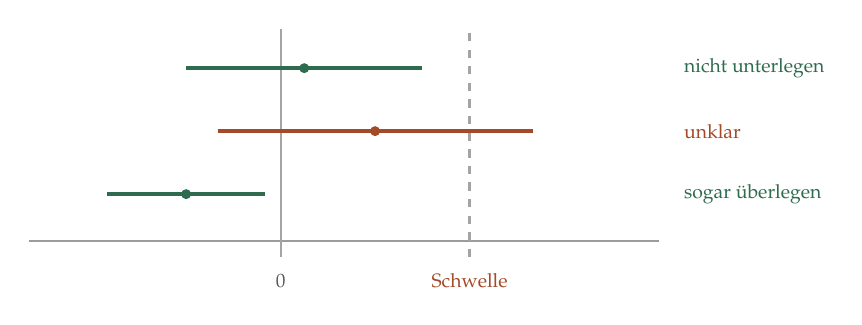
\begin{tikzpicture}[scale=1.0]
\draw[grau!60, line width=0.7pt] (0,0) -- (8.0,0);
\draw[grau!55, dashed, line width=0.8pt] (5.6,-0.2) -- (5.6,2.7);
\draw[grau!55, line width=0.8pt] (3.2,-0.2) -- (3.2,2.7);
\node[font=\scriptsize, color=grau] at (3.2,-0.5) {$0$};
\node[font=\scriptsize, color=akzent] at (5.6,-0.5) {Schwelle};
\draw[gruen, line width=1.5pt] (2.0,2.2) -- (5.0,2.2);
\fill[gruen] (3.5,2.2) circle (1.8pt);
\node[font=\scriptsize, color=gruen, anchor=west] at (8.2,2.2) {nicht unterlegen};
\draw[akzent, line width=1.5pt] (2.4,1.4) -- (6.4,1.4);
\fill[akzent] (4.4,1.4) circle (1.8pt);
\node[font=\scriptsize, color=akzent, anchor=west] at (8.2,1.4) {unklar};
\draw[gruen, line width=1.5pt] (1.0,0.6) -- (3.0,0.6);
\fill[gruen] (2.0,0.6) circle (1.8pt);
\node[font=\scriptsize, color=gruen, anchor=west] at (8.2,0.6) {sogar überlegen};
\end{tikzpicture}
\end{center}
\end{warnung}

\section{Wann darf man auf Ursachen schließen?}

\begin{merksatz}
\boxtitel{Die Kriterien von Bradford Hill}
1965 stellte \Person{Austin Bradford Hill} neun Gesichtspunkte zusammen, die bei der Beurteilung eines beobachteten Zusammenhangs helfen.

\begin{center}
{\small
\renewcommand{\arraystretch}{1.45}
\begin{tabular}{@{}P{0.7cm}P{2.6cm}P{4.8cm}@{}}
\toprule
$1$ & Stärke & Ein starker Zusammenhang ist schwerer durch Störgrößen zu erklären.\\
$2$ & Beständigkeit & Verschiedene Untersucher, Orte, Verfahren finden dasselbe.\\
$3$ & Spezifität & Eine Ursache, eine Wirkung --- schwach, oft verletzt.\\
$4$ & \textbf{Zeitliche Folge} & Die Ursache kommt vor der Wirkung. \textcolor{akzent}{\textbf{Das einzige zwingende Kriterium.}}\\
$5$ & Dosis-Wirkung & Mehr Exposition, mehr Wirkung.\\
$6$ & Plausibilität & Ein Mechanismus ist denkbar.\\
$7$ & Vereinbarkeit & Kein Widerspruch zum sonstigen Wissen.\\
$8$ & Experiment & Wegnahme der Exposition verringert die Wirkung.\\
$9$ & Analogie & Ähnliches ist bekannt.\\
\bottomrule
\end{tabular}}
\end{center}

\begin{center}
\begin{minipage}{0.88\textwidth}
\kursiv{Hill selbst betonte, dies sei \kursiv{keine} Prüfliste zum Abhaken und liefere keine Regel. Genau so wird sie seither benutzt. Die Kriterien sind Gesichtspunkte für ein Urteil, nicht Bedingungen für einen Beweis --- mit der Ausnahme von Nummer vier, die zwingend ist.}
\end{minipage}
\end{center}

\schritt{Am Beispiel Rauchen und Lungenkrebs}
\begin{center}
\renewcommand{\arraystretch}{1.45}
\begin{tabular}{@{}P{2.6cm}P{5.8cm}@{}}
\toprule
Stärke & Relatives Risiko über $10$ --- ungewöhnlich hoch\\
Beständigkeit & Dutzende Studien, viele Länder\\
Zeitliche Folge & Rauchen geht der Erkrankung voraus\\
Dosis-Wirkung & \textcolor{gruen}{deutlich, über mehrere Stufen}\\
Experiment & Aufhören senkt das Risiko\\
\bottomrule
\end{tabular}
\end{center}

Diese Beleglage --- ohne eine einzige randomisierte Studie --- gilt heute als gesichert. Fishers Konfoundereinwand aus Kapitel~5 ließ sich daran abarbeiten.
\end{merksatz}

\section{Übungsaufgaben}

\begin{aufgabe}
\boxtitel{Aufgabe 12.1 --- Verzerrungen erkennen}
Benennen Sie in jedem Fall die Verzerrung und schlagen Sie eine Abhilfe vor.
\begin{center}
{\small
\renewcommand{\arraystretch}{1.4}
\begin{tabular}{@{}P{0.8cm}P{7.6cm}@{}}
\toprule
(a) & Eine Klinik berichtet, ihre neue Operationsmethode habe eine niedrigere Sterblichkeit --- sie wird bei gutem Allgemeinzustand angewandt.\\
(b) & In einer Studie zur Schmerztherapie kennen die Erhebenden die Gruppe.\\
(c) & Eine Studie mit acht Endpunkten berichtet nur den einen, der signifikant war.\\
(d) & Nutzer eines Gesundheitsprogramms leben länger als Nichtnutzer.\\
(e) & Von zwölf Studien zu einem Präparat sind neun veröffentlicht --- alle positiv.\\
\bottomrule
\end{tabular}}
\end{center}

\loesung
\schritt{(a) --- Auswahlverzerrung, hier \kursiv{Indikationsbias}}
Die Methode wird bei günstigeren Fällen eingesetzt. Der Vergleich misst die Auswahl, nicht die Methode.

\kursiv{Abhilfe:} Randomisierung. Notfalls Adjustierung für gemessene Größen --- aber der ungemessene Anteil des Allgemeinzustands bleibt.

\schritt{(b) --- Messverzerrung}
Wer die Gruppe kennt, fragt anders nach Schmerzen und deutet Angaben anders. Bei einem so beeinflussbaren Endpunkt ist das erheblich.

\kursiv{Abhilfe:} verblindete Erhebung durch eine Person, die die Zuteilung nicht kennt.

\schritt{(c) --- Berichtsverzerrung, verstärkt durch Multiplizität}
Bei acht Endpunkten und $\alpha = 0{,}05$ beträgt die Wahrscheinlichkeit für mindestens einen falschen Alarm
\[ 1 - 0{,}95^8 = 1 - 0{,}663 = 0{,}337 . \]
In einem Drittel der Fälle findet man etwas, auch wenn nichts ist.

\kursiv{Abhilfe:} Präregistrierung des primären Endpunkts; Multiplizitätskorrektur (Kapitel~14).

\schritt{(d) --- Verzerrung durch den gesunden Nutzer}
Wer an Gesundheitsprogrammen teilnimmt, unterscheidet sich in vielem: Bildung, Einkommen, Gesundheitsverhalten, Grundzustand. Das Programm wirkt vielleicht --- gemessen wird aber vor allem, wer teilnimmt.

\kursiv{Abhilfe:} Randomisierung der \kursiv{Einladung}, nicht der Teilnahme --- und Auswertung nach Intention-to-treat.

\begin{center}
\begin{minipage}{0.86\textwidth}
\kursiv{Das ist derselbe Gedanke wie bei Screeningprogrammen: Man vergleicht Eingeladene mit Nichteingeladenen, nicht Teilnehmer mit Nichtteilnehmern.}
\end{minipage}
\end{center}

\schritt{(e) --- Publikationsverzerrung}
Die drei unveröffentlichten Studien sind mit hoher Wahrscheinlichkeit die mit ungünstigem Ergebnis. Die Literatur zeichnet ein zu positives Bild.

\kursiv{Abhilfe:} Studienregister mit Pflicht zur Vorabanmeldung; Suche nach unveröffentlichten Daten; Trichterdiagramm in der Metaanalyse (Kapitel~14).
\end{aufgabe}

\begin{aufgabe}
\boxtitel{Aufgabe 12.2 --- Intention-to-treat gegen Per-Protocol}
Eine Studie randomisiert $200$ Personen je Gruppe. In Gruppe A halten alle durch; in Gruppe B brechen $50$ ab, davon haben $10$ Erfolg. Von den $150$ Durchhaltenden haben $105$ Erfolg. In Gruppe A haben $110$ Erfolg.

\loesung
\schritt{Schritt 1 --- Intention-to-treat}
\[ \hat p_A = \frac{110}{200} = 0{,}550 \]
\[ \hat p_B = \frac{105 + 10}{200} = \frac{115}{200} = 0{,}575 \]
\[ \text{Differenz} = 0{,}025 \ \text{--- also } 2{,}5 \text{ Prozentpunkte} \]

\schritt{Schritt 2 --- Per-Protocol}
\[ \hat p_B^{\text{PP}} = \frac{105}{150} = 0{,}700 \]
\[ \text{Differenz} = 0{,}700 - 0{,}550 = 0{,}150 \ \text{--- } 15 \text{ Punkte} \]

\schritt{Schritt 3 --- Der Vergleich}
\begin{center}
\renewcommand{\arraystretch}{1.48}
\begin{tabular}{@{}P{2.8cm}P{1.8cm}P{1.8cm}P{1.8cm}@{}}
\toprule
& $p_A$ & $p_B$ & \textbf{Differenz}\\
\midrule
Intention-to-treat & $0{,}550$ & $0{,}575$ & $\mathbf{0{,}025}$\\
Per-Protocol & $0{,}550$ & $0{,}700$ & $\mathbf{0{,}150}$\\
\bottomrule
\end{tabular}
\end{center}

Sechsfacher Unterschied zwischen beiden Auswertungen.

\schritt{Schritt 4 --- Welche Zahl gilt?}
Die Abbrecher hatten eine Erfolgsrate von $10/50 = 20\,\%$ --- weit unter beiden Gruppen. Sie sind also eine ausgewählte, ungünstige Teilmenge.

Nimmt man sie heraus, bleibt in Gruppe B eine begünstigte Auswahl übrig. In Gruppe A wurde niemand herausgenommen. Der Vergleich ist unfair.

\textbf{Es gilt die Intention-to-treat-Zahl: $2{,}5$ Prozentpunkte.}

\schritt{Schritt 5 --- Was die Abbruchrate bedeutet}
$25\,\%$ Abbrüche in Gruppe B gegen $0\,\%$ in A sind selbst ein Ergebnis --- und zwar ein wichtiges. Die neue Therapie wird von einem Viertel nicht vertragen.

\begin{center}
\begin{minipage}{0.86\textwidth}
\kursiv{Hier zeigt sich, was Intention-to-treat wirklich misst: die Wirkung der Entscheidung, diese Therapie zu beginnen. Sie ist gering --- weil der Vorteil bei den Durchhaltenden durch die Abbrüche fast aufgezehrt wird. Das ist keine Verwässerung, sondern die Wirklichkeit der Versorgung.}
\end{minipage}
\end{center}

\schritt{Schritt 6 --- Was man berichtet}
Beide Zahlen, mit der Abbruchrate, und Intention-to-treat als primäre Auswertung. Die Per-Protocol-Zahl beantwortet eine andere Frage: Wie wirkt die Therapie bei denen, die sie vertragen? Das ist legitim --- aber sie darf nicht als Wirksamkeit der Therapie ausgegeben werden.
\end{aufgabe}

\begin{aufgabe}
\boxtitel{Aufgabe 12.3 --- Eine Studie planen}
Entwerfen Sie das Design für die Frage: \enquote{Verkürzt ein neues Schmerzschema die Zeit bis zur Mobilisation nach Hüftgelenksersatz?}

\loesung
\schritt{Schritt 1 --- Der Typ}
Randomisierte kontrollierte Studie. Die Frage ist eine Wirksamkeitsfrage, die Behandlung ist zuteilbar, der Endpunkt tritt binnen Tagen ein.

\schritt{Schritt 2 --- Die Endpunkte}
\begin{center}
\renewcommand{\arraystretch}{1.48}
\begin{tabular}{@{}P{2.2cm}P{3.0cm}P{2.6cm}@{}}
\toprule
& \textbf{Endpunkt} & \textbf{Skala}\\
\midrule
primär & Zeit bis zur Mobilisation & stetig\\
sekundär & NRS nach 24 h & ordinal\\
sekundär & Bedarfsanalgesie & binär\\
Sicherheit & Nebenwirkungen & binär\\
\bottomrule
\end{tabular}
\end{center}

\textbf{Genau ein primärer Endpunkt.} Jeder weitere erzeugt Multiplizität.

\schritt{Schritt 3 --- Die Mobilisation muss definiert werden}
\enquote{Mobilisiert} ist kein Naturereignis. Man braucht eine überprüfbare Festlegung, etwa: \kursiv{selbständiges Aufstehen und zehn Schritte Gehen mit Gehhilfe, festgestellt durch eine Person, die die Gruppenzuteilung nicht kennt.}

\begin{center}
\begin{minipage}{0.86\textwidth}
\kursiv{Ohne diese Festlegung misst die Studie, wann jemand für mobilisiert erklärt wird --- und das hängt von der Erwartung des Erklärenden ab.}
\end{minipage}
\end{center}

\schritt{Schritt 4 --- Randomisierung}
Blockweise, geschichtet nach Operateur und Altersgruppe. Verdeckte Zuteilung über eine zentrale Stelle.

\schritt{Schritt 5 --- Verblindung}
\begin{center}
\renewcommand{\arraystretch}{1.45}
\begin{tabular}{@{}P{2.6cm}P{2.0cm}P{3.0cm}@{}}
\toprule
& \textbf{möglich?} & \\
\midrule
Personen & \textcolor{mittel}{teilweise} & je nach Applikationsform\\
Behandelnde & \textcolor{akzent}{schwer} & verschiedene Schemata\\
\textbf{Erhebende} & \textcolor{gruen}{\textbf{ja}} & \textcolor{gruen}{\textbf{zwingend}}\\
Auswertende & \textcolor{gruen}{ja} & Gruppen als 1 und 2\\
\bottomrule
\end{tabular}
\end{center}

\schritt{Schritt 6 --- Fallzahl}
Aus Kapitel~7: bei $\sigma = 3{,}5$ Stunden, $\delta = 2{,}0$ Stunden, $\alpha = 0{,}05$, $80\,\%$ Macht:
\[ n = \frac{2 \cdot 7{,}84 \cdot 12{,}25}{4{,}0} = 48 \ \text{je Gruppe} . \]
Mit Reserve für Ausfälle: $60$ je Gruppe.

\schritt{Schritt 7 --- Auswertungsplan, vorab festgelegt}
\begin{center}
\renewcommand{\arraystretch}{1.45}
\begin{tabular}{@{}P{2.4cm}P{5.8cm}@{}}
\toprule
primär & Welch-$t$-Test, zweiseitig, $\alpha = 0{,}05$; Effekt mit $95\,\%$-KI\\
Auswertung & Intention-to-treat\\
sekundär & ohne Anspruch auf Nachweis, ausdrücklich als erkundend gekennzeichnet\\
fehlende Werte & Vorgehen vorab beschreiben\\
\bottomrule
\end{tabular}
\end{center}

\schritt{Schritt 8 --- Vor Beginn}
Anmeldung in einem öffentlichen Studienregister, mit primärem Endpunkt und Auswertungsplan.

\begin{center}
\begin{minipage}{0.86\textwidth}
\kursiv{Dieser letzte Schritt kostet nichts und ist der wirksamste Schutz gegen die Verzerrungen (c) und (e) aus Aufgabe 12.1. Er ist seit 2005 Voraussetzung für die Veröffentlichung in den meisten großen Zeitschriften.}
\end{minipage}
\end{center}
\end{aufgabe}

\begin{geschichte}
\boxtitelg{Von den Zitronen zur Randomisierung}
\Person{James Lind}, Schiffsarzt der britischen Marine, führte 1747 an Bord der \kursiv{HMS Salisbury} einen Versuch durch, der als erste kontrollierte klinische Studie gilt: Zwölf Seeleute mit Skorbut, paarweise auf sechs Behandlungen verteilt --- darunter Zitrusfrüchte.

\begin{center}
\begin{minipage}{0.9\textwidth}
\kursiv{Lind achtete darauf, dass die Zwölf einander im Zustand ähnelten und dieselbe Grundkost erhielten. Die Zuteilung war nicht zufällig, und die Zahl war winzig --- aber der Gedanke der \kursiv{vergleichenden} Prüfung unter gleichen Bedingungen war neu. Die Marine führte die Zitronenration erst 1795 ein, achtundvierzig Jahre später.}
\end{minipage}
\end{center}

\schritt{Die erste randomisierte Studie}
Als solche gilt die Streptomycin-Studie des britischen Medical Research Council von 1948 zur Lungentuberkulose. \Person{Austin Bradford Hill} entwarf sie; die Zuteilung erfolgte über versiegelte Umschläge nach einer Zufallsliste, die nur einer zentralen Stelle bekannt war.

\begin{center}
\begin{minipage}{0.9\textwidth}
\kursiv{Bemerkenswert ist die Begründung, mit der Hill die Randomisierung durchsetzte: Streptomycin war knapp. Nicht alle Erkrankten konnten behandelt werden --- und wenn ohnehin ausgewählt werden musste, dann war das Los die gerechteste und zugleich wissenschaftlich brauchbarste Auswahl.}
\end{minipage}
\end{center}

\schritt{Der Widerstand}
Die Randomisierung setzte sich langsam durch. \Person{Paul Meier} --- derselbe wie in Kapitel~11 --- schrieb noch in den 1970er Jahren gegen die verbreitete Auffassung an, es sei unethisch, die Behandlung dem Zufall zu überlassen.

\begin{center}
\begin{minipage}{0.9\textwidth}
\kursiv{Sein Gegenargument gilt bis heute: Unethisch ist es, Menschen mit einer Behandlung zu versorgen, von der niemand weiß, ob sie wirkt. Der Zustand, in dem beide Möglichkeiten gleich gut begründet sind --- man nennt ihn \Begriff{Gleichgewicht der Ungewissheit} --- ist die Rechtfertigung der Randomisierung und zugleich ihre Grenze: Sobald eine Seite überlegen erscheint, muss die Studie enden.}
\end{minipage}
\end{center}
\end{geschichte}

\begin{forschung}
\boxtitelp{Wohin sich die Studienmethodik bewegt}
\begin{center}
{\small
\renewcommand{\arraystretch}{1.45}
\begin{tabular}{@{}P{2.8cm}P{5.4cm}@{}}
\toprule
\textbf{Pragmatische Studien} & Unter Alltagsbedingungen statt unter Idealbedingungen; breitere Einschlusskriterien, versorgungsnahe Endpunkte.\\
\textbf{Registerbasiert} & Randomisierung innerhalb bestehender Register --- erheblich billiger, große Fallzahlen.\\
\textbf{Adaptive Designs} & Fallzahl oder Gruppenzuteilung werden nach Zwischenauswertung angepasst, mit vorab festgelegten Regeln.\\
\textbf{Plattform\-studien} & Mehrere Therapien gegen eine gemeinsame Kontrolle; neue Arme kommen hinzu, wirkungslose fallen weg.\\
\bottomrule
\end{tabular}}
\end{center}

Die letzte Zeile hat sich während der Pandemie bewährt: Große Plattformstudien prüften in kurzer Zeit zahlreiche Therapien gegen eine gemeinsame Kontrollgruppe und konnten mehrere als wirkungslos ausscheiden --- bei einem Bruchteil des Aufwands getrennter Studien.

\begin{center}
\begin{minipage}{0.88\textwidth}
\kursiv{Adaptive und Plattformdesigns erfordern erheblich mehr methodische Sorgfalt: Jede Zwischenauswertung erzeugt Multiplizität, und jede Anpassungsregel muss vorab festgelegt und in der Fehlerrate berücksichtigt sein. Kapitel~14 behandelt die Grundlagen dafür.}
\end{minipage}
\end{center}

\schritt{Präregistrierung}
Seit 2005 verlangen die großen medizinischen Zeitschriften die Voranmeldung klinischer Studien. Untersuchungen zeigen einen messbaren Effekt: Der Anteil von Studien mit positivem primärem Endpunkt ging in manchen Bereichen deutlich zurück --- ein Hinweis darauf, wie verbreitet das nachträgliche Auswechseln von Endpunkten vorher war.
\end{forschung}

\begin{merksatz}
\boxtitel{Was Sie jetzt können}
\begin{center}
\renewcommand{\arraystretch}{1.5}
\begin{tabular}{@{}P{3.0cm}P{5.6cm}@{}}
\toprule
\textbf{Die Ordnung} & und warum sie keine Rangliste der Wichtigkeit ist\\
\textbf{Randomisierung} & gleicht auch ungemessene Größen aus\\
\textbf{Verdeckte Zuteilung} & ohne sie etwa $30\,\%$ größere Effekte\\
\textbf{Fall-Kontroll} & warum nur das Chancenverhältnis gilt\\
\textbf{Intention-to-treat} & und wann es \kursiv{nicht} konservativ ist\\
\bottomrule
\end{tabular}
\end{center}

\begin{center}
\begin{minipage}{0.88\textwidth}
\kursiv{Im nächsten Kapitel geht es um die Kennzahlen diagnostischer Tests --- und um die Rechnung, die den Fehler aus Kapitel~7 in seiner klinischen Gestalt zeigt.}
\end{minipage}
\end{center}
\end{merksatz}

\chapter{Diagnostische Tests}

\section{Die Vierfeldertafel der Diagnostik}

\begin{merksatz}
\boxtitel{Vier Felder, vier Namen}
\begin{center}
{\small
\renewcommand{\arraystretch}{1.6}
\begin{tabular}{@{}P{2.2cm}P{2.6cm}P{2.6cm}@{}}
\toprule
& \textbf{krank} & \textbf{gesund}\\
\midrule
Test positiv & \textcolor{gruen}{richtig positiv} (RP) & \textcolor{akzent}{falsch positiv} (FP)\\
Test negativ & \textcolor{akzent}{falsch negativ} (FN) & \textcolor{gruen}{richtig negativ} (RN)\\
\bottomrule
\end{tabular}}
\end{center}

\begin{center}
\begin{minipage}{0.88\textwidth}
\kursiv{Die Tafel sieht aus wie die aus Kapitel~7 --- und das ist kein Zufall. Der Fehler erster Art entspricht dem falsch positiven Befund, der zweiter Art dem falsch negativen. Dieses Kapitel zeigt denselben Denkfehler wie dort, nur in klinischer Gestalt.}
\end{minipage}
\end{center}
\end{merksatz}

\begin{definition}
\boxtitelm{Definition 13.1 --- die vier Kennzahlen}
\begin{center}
{\small
\renewcommand{\arraystretch}{1.65}
\begin{tabular}{@{}P{3.4cm}P{2.4cm}P{2.6cm}@{}}
\toprule
\textbf{Name} & \textbf{Formel} & \textbf{Bedingt auf}\\
\midrule
Sensitivität & $\dfrac{\mathrm{RP}}{\mathrm{RP}+\mathrm{FN}}$ & \textbf{Krankheit}\\[6pt]
Spezifität & $\dfrac{\mathrm{RN}}{\mathrm{RN}+\mathrm{FP}}$ & \textbf{Gesundheit}\\[6pt]
Positiver prädiktiver Wert & $\dfrac{\mathrm{RP}}{\mathrm{RP}+\mathrm{FP}}$ & \textbf{Testergebnis}\\[6pt]
Negativer prädiktiver Wert & $\dfrac{\mathrm{RN}}{\mathrm{RN}+\mathrm{FN}}$ & \textbf{Testergebnis}\\
\bottomrule
\end{tabular}}
\end{center}
\end{definition}

\begin{warnung}
\boxtitelr{Die rechte Spalte ist der ganze Punkt}
\begin{center}
\renewcommand{\arraystretch}{1.55}
\begin{tabular}{@{}P{2.6cm}P{6.0cm}@{}}
\toprule
\textbf{Sensitivität} & $\Pr[\text{Test positiv} \mid \text{krank}]$ --- man geht von der Krankheit aus.\\
\textbf{Prädiktiver Wert} & $\Pr[\text{krank} \mid \text{Test positiv}]$ --- man geht vom Befund aus.\\
\bottomrule
\end{tabular}
\end{center}

\begin{center}
\begin{minipage}{0.9\textwidth}
\textbf{Das sind verschiedene Größen, und die Verwechslung ist derselbe Fehler wie bei den sieben Fehldeutungen des $p$-Werts:}
\[ \Pr[D \mid H_0] \quad \text{gegen} \quad \Pr[H_0 \mid D] . \]
\end{minipage}
\end{center}

\begin{center}
\begin{minipage}{0.88\textwidth}
\kursiv{Im Sprechzimmer sitzt niemand, von dem man weiß, dass er krank ist --- man kennt den Befund und sucht die Krankheit. Die Sensitivität beantwortet die umgekehrte Frage. Sie ist eine Eigenschaft des Tests, kein Auskunftsmittel über den Menschen vor einem.}
\end{minipage}
\end{center}
\end{warnung}

\section{Die Prävalenzabhängigkeit --- vorgerechnet}

\begin{merksatz}
\boxtitel{Ein sehr guter Test, drei Lagen}
Wir nehmen einen Test mit
\[ \text{Sensitivität } 99\,\% , \qquad \text{Spezifität } 95\,\% \]
und wenden ihn auf $10\,000$ Personen an --- bei drei verschiedenen Krankheitshäufigkeiten.

\schritt{Lage 1 --- Reihenuntersuchung, Prävalenz $0{,}1\,\%$}
Von $10\,000$ Personen sind $10$ krank und $9990$ gesund.

\begin{center}
\renewcommand{\arraystretch}{1.5}
\begin{tabular}{@{}P{2.2cm}P{2.0cm}P{2.4cm}P{1.8cm}@{}}
\toprule
& \textbf{krank} & \textbf{gesund} & \textbf{Summe}\\
\midrule
positiv & $9{,}9$ & \textcolor{akzent}{$\mathbf{499{,}5}$} & $509{,}4$\\
negativ & $0{,}1$ & $9490{,}5$ & $9490{,}6$\\
\midrule
\textbf{Summe} & $10$ & $9990$ & $10\,000$\\
\bottomrule
\end{tabular}
\end{center}

\kursiv{Die Rechnung:} $10 \cdot 0{,}99 = 9{,}9$ richtig positive; $9990 \cdot 0{,}05 = 499{,}5$ falsch positive.

\[ \mathrm{PPW} = \frac{9{,}9}{509{,}4} = 0{,}0194 \]

\begin{center}
\begin{minipage}{0.9\textwidth}
\textbf{Von hundert positiven Befunden sind etwa zwei richtig.} Achtundneunzig Personen erhalten eine beunruhigende Nachricht und weitere Untersuchungen, ohne krank zu sein.
\end{minipage}
\end{center}

\schritt{Lage 2 --- Verdachtsabklärung, Prävalenz $10\,\%$}
\begin{center}
\renewcommand{\arraystretch}{1.5}
\begin{tabular}{@{}P{2.2cm}P{2.0cm}P{2.0cm}P{1.8cm}@{}}
\toprule
& \textbf{krank} & \textbf{gesund} & \textbf{Summe}\\
\midrule
positiv & $990$ & $450$ & $1440$\\
negativ & $10$ & $8550$ & $8560$\\
\midrule
\textbf{Summe} & $1000$ & $9000$ & $10\,000$\\
\bottomrule
\end{tabular}
\end{center}
\[ \mathrm{PPW} = \frac{990}{1440} = 0{,}688 \]

\schritt{Lage 3 --- begründeter Verdacht, Prävalenz $50\,\%$}
\begin{center}
\renewcommand{\arraystretch}{1.5}
\begin{tabular}{@{}P{2.2cm}P{2.0cm}P{2.0cm}P{1.8cm}@{}}
\toprule
& \textbf{krank} & \textbf{gesund} & \textbf{Summe}\\
\midrule
positiv & $4950$ & $250$ & $5200$\\
negativ & $50$ & $4750$ & $4800$\\
\midrule
\textbf{Summe} & $5000$ & $5000$ & $10\,000$\\
\bottomrule
\end{tabular}
\end{center}
\[ \mathrm{PPW} = \frac{4950}{5200} = 0{,}952 \]

\schritt{Die Zusammenstellung}
\begin{center}
{\small
\renewcommand{\arraystretch}{1.5}
\begin{tabular}{@{}P{2.4cm}P{2.0cm}P{2.0cm}P{1.8cm}@{}}
\toprule
\textbf{Prävalenz} & \textbf{PPW} & \textbf{NPW} & \\
\midrule
$0{,}1\,\%$ & \textcolor{akzent}{$\mathbf{1{,}9\,\%}$} & $99{,}999\,\%$ & \\
$10\,\%$ & $68{,}8\,\%$ & $99{,}9\,\%$ & \\
$50\,\%$ & $95{,}2\,\%$ & $99{,}0\,\%$ & \\
\bottomrule
\end{tabular}}
\end{center}

\begin{center}
\begin{minipage}{0.9\textwidth}
\textbf{Sensitivität und Spezifität sind in allen drei Lagen gleich. Der prädiktive Wert schwankt zwischen zwei und fünfundneunzig Prozent.}
\end{minipage}
\end{center}
\end{merksatz}

\begin{warnung}
\boxtitelr{Woran das liegt --- in einem Satz}
\begin{center}
\begin{minipage}{0.9\textwidth}
Bei einer Prävalenz von $0{,}1\,\%$ gibt es tausendmal mehr Gesunde als Kranke. Selbst wenn nur fünf Prozent der Gesunden fälschlich positiv ausfallen, sind das fünfzigmal mehr Personen, als es Kranke überhaupt gibt.
\end{minipage}
\end{center}

\begin{center}
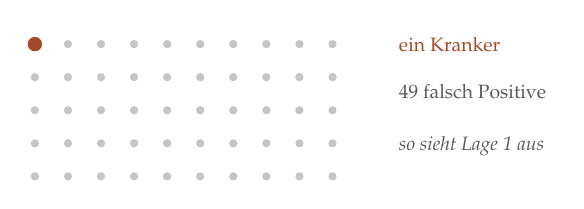
\begin{tikzpicture}[scale=1.0]
\foreach \i in {0,...,49} {
  \pgfmathsetmacro{\xx}{mod(\i,10)*0.42}
  \pgfmathsetmacro{\yy}{-floor(\i/10)*0.42}
  \fill[grau!35] (\xx,\yy) circle (1.5pt);
}
\fill[akzent] (0,0) circle (2.6pt);
\node[font=\scriptsize, color=akzent, anchor=west] at (4.5,0) {ein Kranker};
\node[font=\scriptsize, color=grau, anchor=west] at (4.5,-0.6) {$49$ falsch Positive};
\node[font=\scriptsize\itshape, color=grau, anchor=west] at (4.5,-1.3) {so sieht Lage 1 aus};
\end{tikzpicture}
\end{center}

\begin{center}
\begin{minipage}{0.88\textwidth}
\kursiv{Das ist der Grund, warum Reihenuntersuchungen bei seltenen Krankheiten so schwierig sind. Man braucht eine Spezifität, die weit über $99\,\%$ liegt --- und selbst dann bleibt der prädiktive Wert bescheiden. Kein noch so guter Test kann das Zahlenverhältnis überwinden.}
\end{minipage}
\end{center}
\end{warnung}

\section{Der Satz von Bayes in der handlichen Form}

\begin{merksatz}
\boxtitel{Die Chancenform}
Statt mit Wahrscheinlichkeiten rechnet man handlicher mit Chancen (Definition 11.1).

\begin{center}
\begin{minipage}{0.9\textwidth}
\[ \underbrace{\text{Chance nachher}}_{\text{Nachtest}} \;=\; \underbrace{\text{Chance vorher}}_{\text{Vortest}} \;\times\; \underbrace{\mathrm{LQ}}_{\text{Likelihood-Quotient}} \]
\end{minipage}
\end{center}

\schritt{Die Likelihood-Quotienten}
\[ \mathrm{LQ}^{+} = \frac{\text{Sensitivität}}{1-\text{Spezifität}}, \qquad \mathrm{LQ}^{-} = \frac{1-\text{Sensitivität}}{\text{Spezifität}} \]

\schritt{Für unseren Test}
\[ \mathrm{LQ}^{+} = \frac{0{,}99}{0{,}05} = 19{,}8, \qquad \mathrm{LQ}^{-} = \frac{0{,}01}{0{,}95} = 0{,}0105 \]
\end{merksatz}

\begin{merksatz}
\boxtitel{Lage 1 mit der Chancenform nachgerechnet}
\schritt{Schritt 1 --- Vortestchance}
\[ \text{Chance} = \frac{0{,}001}{0{,}999} = 0{,}001001 \]

\schritt{Schritt 2 --- Multiplizieren}
\[ 0{,}001001 \cdot 19{,}8 = 0{,}019820 \]

\schritt{Schritt 3 --- Zurück in eine Wahrscheinlichkeit}
\[ \pi = \frac{0{,}019820}{1 + 0{,}019820} = \frac{0{,}019820}{1{,}019820} = 0{,}01943 \]

$1{,}94\,\%$ --- wie in der Tafel. \checkmark

\begin{center}
\begin{minipage}{0.88\textwidth}
\kursiv{Der Vorteil dieser Form: Der Likelihood-Quotient hängt \kursiv{nur vom Test} ab, die Vortestchance \kursiv{nur vom Menschen}. Man kann beide getrennt bestimmen und dann multiplizieren --- und man kann mehrere Tests hintereinander schalten, indem man ihre Quotienten multipliziert.}
\end{minipage}
\end{center}
\end{merksatz}

\begin{merksatz}
\boxtitel{Wie stark ein Test ist --- eine Merktabelle}
\begin{center}
{\small
\renewcommand{\arraystretch}{1.48}
\begin{tabular}{@{}P{2.0cm}P{2.6cm}P{3.0cm}@{}}
\toprule
$\mathrm{LQ}^{+}$ & \textbf{Wirkung} & \\
\midrule
$> 10$ & \textcolor{gruen}{große Änderung} & entscheidend\\
$5$ bis $10$ & mäßige Änderung & \\
$2$ bis $5$ & kleine Änderung & \\
$1$ bis $2$ & \textcolor{akzent}{kaum Änderung} & \textcolor{akzent}{nutzlos}\\
$= 1$ & \textcolor{akzent}{keine} & \textcolor{akzent}{der Test sagt nichts}\\
\bottomrule
\end{tabular}}
\end{center}

\begin{center}
\begin{minipage}{0.88\textwidth}
\kursiv{$\mathrm{LQ} = 1$ bedeutet, dass der Befund bei Kranken und Gesunden gleich häufig ist --- der Test trägt nichts bei. Das kommt häufiger vor, als man denkt, besonders bei Befunden mit mäßiger Spezifität.}
\end{minipage}
\end{center}
\end{merksatz}

\section{Die ROC-Kurve}

\begin{merksatz}
\boxtitel{Wenn der Test eine Zahl liefert}
Die meisten Tests messen eine stetige Größe und vergleichen sie mit einer Schwelle. Die Schwelle ist frei wählbar --- und jede Wahl liefert ein anderes Paar aus Sensitivität und Spezifität.

\begin{center}
\renewcommand{\arraystretch}{1.5}
\begin{tabular}{@{}P{2.6cm}P{2.6cm}P{2.8cm}@{}}
\toprule
\textbf{Schwelle} & \textbf{Sensitivität} & \textbf{Spezifität}\\
\midrule
sehr niedrig & \textcolor{gruen}{hoch} & \textcolor{akzent}{niedrig}\\
mittel & mittel & mittel\\
sehr hoch & \textcolor{akzent}{niedrig} & \textcolor{gruen}{hoch}\\
\bottomrule
\end{tabular}
\end{center}

\begin{center}
\begin{minipage}{0.9\textwidth}
\textbf{Man kann beides nicht gleichzeitig maximieren.} Die ROC-Kurve macht diesen Tauschhandel sichtbar: Sie trägt die Sensitivität gegen $1-$Spezifität auf, für alle möglichen Schwellen.
\end{minipage}
\end{center}

\begin{center}
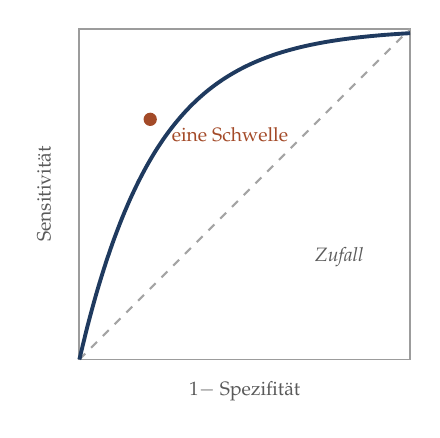
\begin{tikzpicture}[scale=1.0]
\draw[grau!60, line width=0.7pt] (0,0) rectangle (4.2,4.2);
\draw[grau!55, dashed, line width=0.8pt] (0,0) -- (4.2,4.2);
\draw[tief, line width=1.4pt] plot[smooth, samples=40, domain=0:4.2]
  (\x, {4.2*(1-exp(-1.35*\x/4.2*3.2))});
\fill[akzent] (0.9,3.05) circle (2.4pt);
\node[font=\scriptsize, color=akzent, anchor=west] at (1.05,2.85) {eine Schwelle};
\node[font=\scriptsize, color=grau] at (2.1,-0.4) {$1 - $ Spezifität};
\node[font=\scriptsize, color=grau, rotate=90] at (-0.45,2.1) {Sensitivität};
\node[font=\scriptsize\itshape, color=grau] at (3.3,1.3) {Zufall};
\end{tikzpicture}
\end{center}
\end{merksatz}

\begin{definition}
\boxtitelm{Definition 13.2 --- die Fläche unter der Kurve}
Die \Begriff{AUC} ist die Fläche unter der ROC-Kurve. Sie liegt zwischen $0{,}5$ (Zufall) und $1$ (vollkommene Trennung).
\end{definition}

\begin{merksatz}
\boxtitel{Was die AUC bedeutet --- und die Verbindung zu Kapitel~9}
\begin{center}
\begin{minipage}{0.9\textwidth}
\textbf{Die AUC ist die Wahrscheinlichkeit, dass eine zufällig gewählte kranke Person einen höheren Testwert hat als eine zufällig gewählte gesunde.}
\end{minipage}
\end{center}

\schritt{Die Verbindung}
Das ist genau die Überlegenheitswahrscheinlichkeit aus Kapitel~9:
\[ \mathrm{AUC} = \frac{U}{n_1 \cdot n_2} . \]
Die AUC und der Mann-Whitney-Test messen dieselbe Größe.

\begin{center}
{\small
\renewcommand{\arraystretch}{1.48}
\begin{tabular}{@{}P{2.0cm}P{3.0cm}P{2.6cm}@{}}
\toprule
\textbf{AUC} & \textbf{Beurteilung} & \\
\midrule
$0{,}5$ & Zufall & nutzlos\\
$0{,}6$--$0{,}7$ & schwach & \\
$0{,}7$--$0{,}8$ & brauchbar & \\
$0{,}8$--$0{,}9$ & gut & \\
$> 0{,}9$ & sehr gut & \textcolor{mittel}{Verdacht prüfen}\\
\bottomrule
\end{tabular}}
\end{center}

\begin{center}
\begin{minipage}{0.88\textwidth}
\kursiv{Die letzte Zeile ist ernst gemeint: Eine AUC über $0{,}95$ in einer klinischen Anwendung ist häufiger ein Hinweis auf einen Fehler im Aufbau --- etwa dass der Testwert in die Referenzdiagnose eingeflossen ist --- als auf einen außergewöhnlichen Test.}
\end{minipage}
\end{center}
\end{merksatz}

\begin{warnung}
\boxtitelr{Was die AUC nicht leistet}
\begin{center}
\renewcommand{\arraystretch}{1.52}
\begin{tabular}{@{}P{2.6cm}P{6.0cm}@{}}
\toprule
\textbf{Keine Schwelle} & Sie fasst alle Schwellen zusammen --- auch die unbrauchbaren. Für die Praxis braucht man eine.\\
\textbf{Keine Gewichtung} & Sie behandelt falsch positive und falsch negative Befunde gleich. In der Wirklichkeit sind sie es selten.\\
\textbf{Keine Prävalenz} & Wie Sensitivität und Spezifität ist sie prävalenzunabhängig --- und sagt deshalb nichts über den prädiktiven Wert.\\
\bottomrule
\end{tabular}
\end{center}
\end{warnung}

\begin{merksatz}
\boxtitel{Wie man die Schwelle wählt}
Nicht rechnerisch, sondern nach den Folgen der beiden Fehler.

\begin{center}
{\small
\renewcommand{\arraystretch}{1.5}
\begin{tabular}{@{}P{3.0cm}P{2.2cm}P{3.0cm}@{}}
\toprule
\textbf{Lage} & \textbf{Wichtiger} & \textbf{Schwelle}\\
\midrule
Ausschluss einer bedrohlichen Krankheit & Sensitivität & niedrig\\
Bestätigung vor eingreifender Therapie & Spezifität & hoch\\
Blutspende-Prüfung & Sensitivität & sehr niedrig\\
Reihen\-untersuchung & Spezifität & \textcolor{akzent}{hoch --- wegen der Prävalenz}\\
\bottomrule
\end{tabular}}
\end{center}

\begin{center}
\begin{minipage}{0.88\textwidth}
\kursiv{Die häufig empfohlene Wahl \enquote{der Punkt mit dem größten Abstand zur Diagonale} --- der Youden-Index --- setzt stillschweigend voraus, dass beide Fehler gleich schwer wiegen und die Prävalenz bei fünfzig Prozent liegt. Beides trifft fast nie zu.}
\end{minipage}
\end{center}
\end{merksatz}

\section{Reihenuntersuchungen}

\begin{warnung}
\boxtitelr{Drei Größen, die man nennen muss}
\begin{center}
{\small
\renewcommand{\arraystretch}{1.52}
\begin{tabular}{@{}P{2.8cm}P{5.8cm}@{}}
\toprule
\textbf{Zahl der nötigen Untersuchungen} & Wie viele Personen müssen untersucht werden, um einen Todesfall zu verhindern?\\
\textbf{Falsch positive je Fund} & Aus den Rechnungen oben: bei niedriger Prävalenz oft mehrere Dutzend.\\
\textbf{Überdiagnose} & Anteil der entdeckten Fälle, die nie Beschwerden verursacht hätten.\\
\bottomrule
\end{tabular}}
\end{center}

\schritt{Zur Überdiagnose}
Sie ist die schwierigste der drei, weil man sie am Einzelnen nie feststellen kann: Man weiß nicht, ob dieser entdeckte Befund je Beschwerden gemacht hätte.

Nachweisbar ist sie nur im Vergleich: Findet man in der untersuchten Gruppe dauerhaft mehr Fälle als in der nicht untersuchten, ohne dass die Sterblichkeit entsprechend sinkt, so ist die Differenz Überdiagnose.

\begin{center}
\begin{minipage}{0.88\textwidth}
\kursiv{Jede Überdiagnose führt zu einer Behandlung, die nur schaden kann --- denn der Befund hätte nie geschadet. Das ist kein Argument gegen Früherkennung, sondern eines dafür, Nutzen und Schaden gemeinsam zu beziffern. Die Zahlen dafür liegen für die großen Programme vor; sie werden in der Beratung selten genannt.}
\end{minipage}
\end{center}
\end{warnung}

\section{Übungsaufgaben}

\begin{aufgabe}
\boxtitel{Aufgabe 13.1 --- Prädiktive Werte berechnen}
Ein Test hat eine Sensitivität von $90\,\%$ und eine Spezifität von $85\,\%$. Berechnen Sie beide prädiktiven Werte bei Prävalenzen von $1\,\%$, $20\,\%$ und $60\,\%$.

\loesung
\schritt{Schritt 1 --- Prävalenz $1\,\%$}
Von $10\,000$: $100$ krank, $9900$ gesund.
\begin{center}
\renewcommand{\arraystretch}{1.45}
\begin{tabular}{@{}P{2.0cm}P{1.8cm}P{1.8cm}P{1.8cm}@{}}
\toprule
& \textbf{krank} & \textbf{gesund} & \textbf{Summe}\\
\midrule
positiv & $90$ & $1485$ & $1575$\\
negativ & $10$ & $8415$ & $8425$\\
\bottomrule
\end{tabular}
\end{center}
\kursiv{Rechnung:} $100 \cdot 0{,}90 = 90$; $9900 \cdot 0{,}15 = 1485$.
\[ \mathrm{PPW} = \frac{90}{1575} = 0{,}0571, \qquad \mathrm{NPW} = \frac{8415}{8425} = 0{,}9988 \]

\schritt{Schritt 2 --- Prävalenz $20\,\%$}
$2000$ krank, $8000$ gesund.
\begin{center}
\renewcommand{\arraystretch}{1.45}
\begin{tabular}{@{}P{2.0cm}P{1.8cm}P{1.8cm}P{1.8cm}@{}}
\toprule
& \textbf{krank} & \textbf{gesund} & \textbf{Summe}\\
\midrule
positiv & $1800$ & $1200$ & $3000$\\
negativ & $200$ & $6800$ & $7000$\\
\bottomrule
\end{tabular}
\end{center}
\[ \mathrm{PPW} = \frac{1800}{3000} = 0{,}600, \qquad \mathrm{NPW} = \frac{6800}{7000} = 0{,}971 \]

\schritt{Schritt 3 --- Prävalenz $60\,\%$}
$6000$ krank, $4000$ gesund.
\begin{center}
\renewcommand{\arraystretch}{1.45}
\begin{tabular}{@{}P{2.0cm}P{1.8cm}P{1.8cm}P{1.8cm}@{}}
\toprule
& \textbf{krank} & \textbf{gesund} & \textbf{Summe}\\
\midrule
positiv & $5400$ & $600$ & $6000$\\
negativ & $600$ & $3400$ & $4000$\\
\bottomrule
\end{tabular}
\end{center}
\[ \mathrm{PPW} = \frac{5400}{6000} = 0{,}900, \qquad \mathrm{NPW} = \frac{3400}{4000} = 0{,}850 \]

\schritt{Schritt 4 --- Die Übersicht}
\begin{center}
\renewcommand{\arraystretch}{1.48}
\begin{tabular}{@{}P{2.2cm}P{2.0cm}P{2.0cm}P{2.0cm}@{}}
\toprule
\textbf{Prävalenz} & \textbf{PPW} & \textbf{NPW} & \\
\midrule
$1\,\%$ & $5{,}7\,\%$ & $99{,}9\,\%$ & \\
$20\,\%$ & $60{,}0\,\%$ & $97{,}1\,\%$ & \\
$60\,\%$ & $90{,}0\,\%$ & $85{,}0\,\%$ & \\
\bottomrule
\end{tabular}
\end{center}

\schritt{Schritt 5 --- Die Beobachtung}
Die beiden prädiktiven Werte bewegen sich \kursiv{gegenläufig}. Bei niedriger Prävalenz ist der negative Wert hervorragend und der positive fast wertlos; bei hoher Prävalenz umgekehrt.

\begin{center}
\begin{minipage}{0.86\textwidth}
\kursiv{Daraus folgt eine praktische Regel: \textbf{Ein Test ist dort am nützlichsten, wo man am unsichersten ist.} Bei sehr niedriger oder sehr hoher Vortestwahrscheinlichkeit ändert er die Einschätzung kaum --- und man hätte auf ihn verzichten können.}
\end{minipage}
\end{center}
\end{aufgabe}

\begin{aufgabe}
\boxtitel{Aufgabe 13.2 --- Zwei Tests nacheinander}
Eine Person hat eine Vortestwahrscheinlichkeit von $20\,\%$. Test~1 ($\mathrm{LQ}^{+} = 6$) fällt positiv aus, Test~2 ($\mathrm{LQ}^{+} = 4$) ebenfalls. Wie hoch ist die Wahrscheinlichkeit danach?

\loesung
\schritt{Schritt 1 --- Vortestchance}
\[ \frac{0{,}20}{0{,}80} = 0{,}25 \]

\schritt{Schritt 2 --- Nach Test 1}
\[ 0{,}25 \cdot 6 = 1{,}50 \quad\Longrightarrow\quad \pi = \frac{1{,}50}{2{,}50} = 0{,}600 \]

\schritt{Schritt 3 --- Nach Test 2}
\[ 1{,}50 \cdot 4 = 6{,}00 \quad\Longrightarrow\quad \pi = \frac{6{,}00}{7{,}00} = 0{,}857 \]

\schritt{Antwort}
Etwa $\mathbf{86\,\%}$.

\schritt{Schritt 4 --- Die Kurzfassung}
Da sich die Quotienten multiplizieren, geht es auch in einem Schritt:
\[ 0{,}25 \cdot 6 \cdot 4 = 0{,}25 \cdot 24 = 6{,}00 . \quad \checkmark \]

\schritt{Schritt 5 --- Die stillschweigende Voraussetzung}
\begin{center}
\begin{minipage}{0.9\textwidth}
\textbf{Die Multiplikation setzt voraus, dass die beiden Tests \kursiv{bedingt unabhängig} sind} --- dass also Test~2 bei einer kranken Person nicht deshalb häufiger positiv ausfällt, weil Test~1 es war.
\end{minipage}
\end{center}

Diese Voraussetzung ist oft verletzt. Zwei Tests, die denselben zugrundeliegenden Vorgang messen --- etwa zwei Entzündungsparameter ---, sind stark voneinander abhängig. Der zweite bringt dann viel weniger als sein Quotient verspricht.

\begin{center}
\begin{minipage}{0.86\textwidth}
\kursiv{Praktisch bedeutet das: Wer zwei ähnliche Tests hintereinanderschaltet und ihre Quotienten multipliziert, überschätzt die gewonnene Sicherheit --- unter Umständen erheblich. Zwei \kursiv{verschiedenartige} Verfahren --- etwa ein Laborwert und ein bildgebender Befund --- sind eher unabhängig.}
\end{minipage}
\end{center}

\schritt{Schritt 6 --- Ein Gegenprobe-Gedanke}
Wäre Test~2 mit Test~1 vollständig gekoppelt, so brächte er gar nichts: Die Wahrscheinlichkeit bliebe bei $60\,\%$. Die Wahrheit liegt meist dazwischen.
\end{aufgabe}

\begin{aufgabe}
\boxtitel{Aufgabe 13.3 --- Eine Schwelle wählen}
Ein Wert soll zwischen Personen mit und ohne eine Erkrankung trennen. Fünf mögliche Schwellen liefern:
\begin{center}
{\small
\renewcommand{\arraystretch}{1.4}
\begin{tabular}{@{}P{1.6cm}P{2.0cm}P{2.0cm}P{2.0cm}@{}}
\toprule
\textbf{Schwelle} & \textbf{Sens.} & \textbf{Spez.} & $\mathrm{LQ}^{+}$\\
\midrule
$A$ & $0{,}99$ & $0{,}40$ & \\
$B$ & $0{,}95$ & $0{,}70$ & \\
$C$ & $0{,}85$ & $0{,}85$ & \\
$D$ & $0{,}70$ & $0{,}95$ & \\
$E$ & $0{,}40$ & $0{,}99$ & \\
\bottomrule
\end{tabular}}
\end{center}
Ergänzen Sie die Quotienten und wählen Sie für zwei Lagen begründet eine Schwelle.

\loesung
\schritt{Schritt 1 --- Die Quotienten}
\begin{center}
{\small
\renewcommand{\arraystretch}{1.42}
\begin{tabular}{@{}P{1.4cm}P{1.8cm}P{1.8cm}P{1.8cm}P{1.6cm}@{}}
\toprule
& \textbf{Sens.} & \textbf{Spez.} & $\mathrm{LQ}^{+}$ & $\mathrm{LQ}^{-}$\\
\midrule
$A$ & $0{,}99$ & $0{,}40$ & $1{,}65$ & $\mathbf{0{,}025}$\\
$B$ & $0{,}95$ & $0{,}70$ & $3{,}17$ & $0{,}071$\\
$C$ & $0{,}85$ & $0{,}85$ & $5{,}67$ & $0{,}176$\\
$D$ & $0{,}70$ & $0{,}95$ & $14{,}0$ & $0{,}316$\\
$E$ & $0{,}40$ & $0{,}99$ & $\mathbf{40{,}0}$ & $0{,}606$\\
\bottomrule
\end{tabular}}
\end{center}

\kursiv{Zur Rechnung:} $\mathrm{LQ}^{+}_A = 0{,}99/0{,}60 = 1{,}65$; $\mathrm{LQ}^{-}_A = 0{,}01/0{,}40 = 0{,}025$.

\schritt{Schritt 2 --- Lage 1: Ausschluss einer bedrohlichen Erkrankung}
Hier will man sicher sein, niemanden zu übersehen. Maßgeblich ist $\mathrm{LQ}^{-}$: Er soll möglichst klein sein, damit ein negativer Befund die Wahrscheinlichkeit stark senkt.

\textbf{Wahl: Schwelle $A$} mit $\mathrm{LQ}^{-} = 0{,}025$.

\kursiv{Wirkung:} Bei einer Vortestwahrscheinlichkeit von $10\,\%$ --- Chance $0{,}111$ --- führt ein negativer Befund zu
\[ 0{,}111 \cdot 0{,}025 = 0{,}00278 \quad\Longrightarrow\quad \pi = 0{,}0028 , \]
also $0{,}3\,\%$. Die Erkrankung ist praktisch ausgeschlossen.

\kursiv{Der Preis:} Die Spezifität von $0{,}40$ bedeutet, dass $60\,\%$ der Gesunden positiv ausfallen und weiter abgeklärt werden müssen.

\schritt{Schritt 3 --- Lage 2: Bestätigung vor einem eingreifenden Verfahren}
Hier will man sicher sein, niemanden ohne Grund zu operieren. Maßgeblich ist $\mathrm{LQ}^{+}$.

\textbf{Wahl: Schwelle $E$} mit $\mathrm{LQ}^{+} = 40$.

\kursiv{Wirkung:} Bei Vortestwahrscheinlichkeit $30\,\%$ --- Chance $0{,}4286$ ---:
\[ 0{,}4286 \cdot 40 = 17{,}14 \quad\Longrightarrow\quad \pi = \frac{17{,}14}{18{,}14} = 0{,}945 \]
$94{,}5\,\%$ --- eine belastbare Grundlage für den Eingriff.

\kursiv{Der Preis:} Die Sensitivität von $0{,}40$ bedeutet, dass sechzig Prozent der Erkrankten nicht erkannt werden.

\schritt{Schritt 4 --- Die Lehre}
\begin{center}
\renewcommand{\arraystretch}{1.48}
\begin{tabular}{@{}P{2.6cm}P{2.4cm}P{2.8cm}@{}}
\toprule
\textbf{Zweck} & \textbf{Schwelle} & \textbf{Maßgeblich}\\
\midrule
Ausschließen & niedrig ($A$) & $\mathrm{LQ}^{-}$\\
Bestätigen & hoch ($E$) & $\mathrm{LQ}^{+}$\\
Beides mäßig & mittel ($C$) & \\
\bottomrule
\end{tabular}
\end{center}

\begin{center}
\begin{minipage}{0.86\textwidth}
\kursiv{Derselbe Test mit derselben ROC-Kurve leistet Verschiedenes, je nachdem wo man schneidet. Und die Wahl folgt nicht aus der Kurve, sondern aus der Frage --- das ist dieselbe Einsicht wie in Kapitel~1: Die Rechnung sagt nicht, wozu sie dient.}
\end{minipage}
\end{center}

\schritt{Schritt 5 --- Warum man beide Schwellen benutzen kann}
In der Praxis verwendet man oft \kursiv{zwei} Schwellen: Unterhalb von $A$ gilt die Erkrankung als ausgeschlossen, oberhalb von $E$ als bestätigt, dazwischen ist der Befund unklar und es folgt weitere Diagnostik.

Das ist ehrlicher als eine einzelne Schwelle, weil es den mittleren Bereich als das ausweist, was er ist: unentschieden.
\end{aufgabe}

\begin{geschichte}
\boxtitelg{Ein Geistlicher, ein Radargerät und ein später Ruhm}
\Person{Thomas Bayes} (etwa 1702--1761) war presbyterianischer Geistlicher in Tunbridge Wells. Seine Arbeit über die umgekehrte Wahrscheinlichkeit erschien 1763, zwei Jahre nach seinem Tod, eingereicht von seinem Freund Richard Price.

\begin{center}
\begin{minipage}{0.9\textwidth}
\kursiv{Bayes selbst hatte sie nicht veröffentlicht --- vermutlich, weil er ihre Bedeutung nicht erkannte. Die allgemeine Form und die ersten Anwendungen stammen von \Person{Pierre-Simon Laplace}, der sie um 1774 unabhängig entwickelte und über Jahrzehnte ausbaute.}
\end{minipage}
\end{center}

\schritt{Die ROC-Kurve kommt aus dem Krieg}
Der Name steht für \kursiv{receiver operating characteristic}. Er stammt aus der Radartechnik des Zweiten Weltkriegs: Operateure mussten entscheiden, ob ein Ausschlag auf dem Schirm ein Flugzeug war oder Rauschen.

Die Frage war dieselbe wie in der Diagnostik: Wo setzt man die Schwelle, und wie tauscht man Treffer gegen Fehlalarme? Die Kurve wurde in den 1950er Jahren in die Psychophysik übernommen und gelangte erst um 1970 in die Medizin.

\begin{center}
\begin{minipage}{0.9\textwidth}
\kursiv{Die Herkunft erklärt einen Zug der Methode, der in der Medizin fremd wirkt: Sie behandelt den Beurteiler als Teil des Systems. Wo die Schwelle liegt, ist eine Entscheidung des Operateurs --- nicht eine Eigenschaft des Geräts.}
\end{minipage}
\end{center}
\end{geschichte}

\begin{forschung}
\boxtitelp{Was bei diagnostischen Studien heute schiefgeht}
\begin{center}
{\small
\renewcommand{\arraystretch}{1.45}
\begin{tabular}{@{}P{2.8cm}P{5.4cm}@{}}
\toprule
\textbf{Spektrumbias} & Werden schwer Erkrankte mit Gesunden verglichen, erscheint der Test viel besser als in der Praxis, wo die Grenzfälle überwiegen.\\
\textbf{Verifikationsbias} & Wird die Referenzdiagnose nur bei positivem Test erhoben, verzerrt das beide Kennzahlen.\\
\textbf{Fehlende Schwelle} & Wird die Schwelle nachträglich an denselben Daten optimiert, sind Sensitivität und Spezifität zu gut.\\
\bottomrule
\end{tabular}}
\end{center}

Die STARD-Empfehlungen --- zuletzt 2015 überarbeitet --- verlangen, alle drei Punkte offenzulegen. Die Befolgung ist unvollständig.

\schritt{Maschinelles Lernen in der Bildgebung}
Seit etwa 2018 erscheinen zahlreiche Arbeiten zu lernenden Systemen in der Diagnostik, oft mit AUC-Werten über $0{,}95$.

\begin{center}
{\small
\renewcommand{\arraystretch}{1.45}
\begin{tabular}{@{}P{2.6cm}P{5.6cm}@{}}
\toprule
\textbf{Die Frage} & Wie gut ist das System an \kursiv{fremden} Daten, aus anderen Geräten und Kliniken?\\
\textbf{Der Befund} & Die Leistung fällt bei externer Prüfung regelmäßig deutlich ab.\\
\textbf{Der Grund} & Systeme lernen Merkmale des Aufnahmeorts mit --- Gerätetyp, Lagerung, Beschriftung.\\
\bottomrule
\end{tabular}}
\end{center}

\begin{center}
\begin{minipage}{0.88\textwidth}
\kursiv{Übersichtsarbeiten kommen übereinstimmend zu dem Schluss, dass nur ein kleiner Teil der veröffentlichten Systeme extern geprüft wurde. Und selbst ein gut geprüftes System unterliegt der Rechnung dieses Kapitels: Bei niedriger Prävalenz bleibt der prädiktive Wert bescheiden, wie gut die AUC auch sei.}
\end{minipage}
\end{center}
\end{forschung}

\begin{merksatz}
\boxtitel{Was Sie jetzt können}
\begin{center}
\renewcommand{\arraystretch}{1.5}
\begin{tabular}{@{}P{3.2cm}P{5.4cm}@{}}
\toprule
\textbf{Definition 13.1} & vier Kennzahlen --- und worauf jede bedingt\\
\textbf{Prävalenz} & derselbe Test: PPW von $2$ bis $95\,\%$\\
\textbf{Chancenform} & Vortestchance $\times$ Likelihood-Quotient\\
\textbf{Definition 13.2} & AUC --- dieselbe Größe wie Mann-Whitneys $U$\\
\textbf{Schwellenwahl} & folgt aus der Frage, nicht aus der Kurve\\
\bottomrule
\end{tabular}
\end{center}

\begin{center}
\begin{minipage}{0.88\textwidth}
\kursiv{Im nächsten Kapitel geht es um das, was geschieht, wenn man viele Fragen zugleich stellt --- und darum, wie man Ergebnisse vieler Studien zusammenfasst.}
\end{minipage}
\end{center}
\end{merksatz}

\chapter{Viele Tests auf einmal}

\section{Das Problem}

\begin{merksatz}
\boxtitel{Die Rechnung aus Kapitel~8, allgemein}
Führt man $m$ unabhängige Tests zum Niveau $\alpha$ durch und trifft keine einzige Alternativhypothese zu, so ist die Wahrscheinlichkeit für mindestens einen falschen Alarm
\[ 1 - (1-\alpha)^m . \]

\begin{center}
{\small
\renewcommand{\arraystretch}{1.48}
\begin{tabular}{@{}P{1.8cm}P{2.4cm}P{3.0cm}@{}}
\toprule
$m$ & \textbf{Fehlerrate} & \\
\midrule
$1$ & $5{,}0\,\%$ & \\
$5$ & $22{,}6\,\%$ & \\
$10$ & $40{,}1\,\%$ & \\
$20$ & $64{,}2\,\%$ & \\
$100$ & \textcolor{akzent}{$\mathbf{99{,}4\,\%}$} & \textcolor{akzent}{fast sicher}\\
\bottomrule
\end{tabular}}
\end{center}

\begin{center}
\begin{minipage}{0.88\textwidth}
\kursiv{Bei hundert geprüften Zusammenhängen findet man praktisch sicher etwas --- auch wenn nichts vorhanden ist. Und man findet im Mittel fünf davon.}
\end{minipage}
\end{center}
\end{merksatz}

\begin{warnung}
\boxtitelr{Wo Multiplizität entsteht --- oft unbemerkt}
\begin{center}
{\small
\renewcommand{\arraystretch}{1.5}
\begin{tabular}{@{}P{3.0cm}P{5.6cm}@{}}
\toprule
\textbf{Mehrere End\-punkte} & Schmerz, Mobilisation, Zufriedenheit, Liegedauer, Nebenwirkungen.\\
\textbf{Mehrere Gruppen} & Drei Therapien ergeben drei Paarvergleiche.\\
\textbf{Mehrere Zeitpunkte} & Messung nach $6$, $12$, $24$, $48$ Stunden.\\
\textbf{Untergruppen} & Männer, Frauen, Alt, Jung, mit und ohne Begleiterkrankung.\\
\textbf{Zwischen\-auswertungen} & Jeder Blick in die laufenden Daten ist ein Test.\\
\textbf{\textcolor{akzent}{Verfahrens\-wahl}} & \textcolor{akzent}{Wer $t$-Test und Mann-Whitney rechnet und den kleineren berichtet, hat zweimal getestet.}\\
\bottomrule
\end{tabular}}
\end{center}

\begin{center}
\begin{minipage}{0.88\textwidth}
\kursiv{Die letzte Zeile ist die unsichtbarste. Sie erscheint in keiner Veröffentlichung, weil nur das gewählte Verfahren berichtet wird --- und sie ist genau die Lage aus Aufgabe 9.1, wo $t$-Test und Rangtest zu verschiedenen Schlüssen führten.}
\end{minipage}
\end{center}
\end{warnung}

\section{Die Korrekturverfahren}

\begin{definition}
\boxtitelm{Definition 14.1 --- zwei Fehlerbegriffe}
\begin{center}
{\small
\renewcommand{\arraystretch}{1.55}
\begin{tabular}{@{}P{3.4cm}P{5.2cm}@{}}
\toprule
\textbf{Familienweise Fehlerrate} & Die Wahrscheinlichkeit, \kursiv{mindestens einen} falschen Alarm unter allen Tests zu haben.\\
\textbf{Falscher\-kennungsrate} & Der erwartete \kursiv{Anteil} falscher Alarme unter den als signifikant erklärten Ergebnissen.\\
\bottomrule
\end{tabular}}
\end{center}
\end{definition}

\begin{merksatz}
\boxtitel{Bonferroni}
Man prüft jeden Test gegen $\alpha/m$ statt gegen $\alpha$.

\schritt{Warum das genügt}
Die Wahrscheinlichkeit einer Vereinigung ist höchstens die Summe der Einzelwahrscheinlichkeiten:
\[ \Pr\Bigl[\bigcup_{i} \{\text{Test } i \text{ schlägt falsch an}\}\Bigr] \;\le\; \sum_{i=1}^m \frac{\alpha}{m} = \alpha . \]

Diese Abschätzung braucht \kursiv{keine} Unabhängigkeit --- das ist ihre Stärke.

\schritt{Die Schwäche}
Sie ist grob. Bei abhängigen Tests ist die tatsächliche Fehlerrate deutlich kleiner als $\alpha$, und man verliert entsprechend Macht.
\end{merksatz}

\begin{merksatz}
\boxtitel{Holm --- dasselbe Niveau, mehr Macht}
\begin{center}
\renewcommand{\arraystretch}{1.5}
\begin{tabular}{@{}P{1.0cm}P{7.4cm}@{}}
\toprule
$1$ & $p$-Werte aufsteigend sortieren: $p_{(1)} \le \cdots \le p_{(m)}$.\\
$2$ & $p_{(1)}$ gegen $\alpha/m$ prüfen. Nicht signifikant $\Rightarrow$ abbrechen.\\
$3$ & $p_{(2)}$ gegen $\alpha/(m-1)$ prüfen. Und so fort.\\
$4$ & Beim ersten Nichtbestehen abbrechen; alle weiteren gelten als nicht signifikant.\\
\bottomrule
\end{tabular}
\end{center}

\begin{center}
\begin{minipage}{0.9\textwidth}
\textbf{Holm hält dieselbe familienweise Fehlerrate ein wie Bonferroni und verwirft nie weniger --- oft mehr.} Es gibt daher keinen Grund, Bonferroni zu verwenden.
\end{minipage}
\end{center}

\begin{center}
\begin{minipage}{0.88\textwidth}
\kursiv{Dass Bonferroni trotzdem der bekanntere Name ist, hat denselben Grund wie bei Student gegen Welch in Kapitel~8: Er ist älter und einfacher zu erklären.}
\end{minipage}
\end{center}
\end{merksatz}

\begin{merksatz}
\boxtitel{Benjamini und Hochberg --- ein anderes Ziel}
Statt \kursiv{keinen} falschen Alarm zuzulassen, erlaubt man einen festen \kursiv{Anteil}.

\begin{center}
\renewcommand{\arraystretch}{1.5}
\begin{tabular}{@{}P{1.0cm}P{7.4cm}@{}}
\toprule
$1$ & $p$-Werte aufsteigend sortieren.\\
$2$ & Das größte $i$ suchen mit $p_{(i)} \le \dfrac{i}{m}\,q$.\\
$3$ & Alle Tests bis einschließlich $i$ verwerfen.\\
\bottomrule
\end{tabular}
\end{center}

\begin{center}
\begin{minipage}{0.88\textwidth}
\kursiv{Bei $q = 0{,}05$ heißt das: Unter den als signifikant erklärten Ergebnissen sind im Mittel fünf Prozent falsch. Das ist ein anderer Anspruch als \enquote{höchstens fünf Prozent Wahrscheinlichkeit für einen einzigen Fehler} --- deutlich schwächer, und bei vielen Tests der brauchbarere.}
\end{minipage}
\end{center}
\end{merksatz}

\begin{merksatz}
\boxtitel{Die drei Verfahren an denselben Zahlen}
Fünf Tests mit
\[ p = 0{,}003,\quad 0{,}011,\quad 0{,}021,\quad 0{,}038,\quad 0{,}045 \]
und $\alpha = q = 0{,}05$.

\begin{center}
{\small
\renewcommand{\arraystretch}{1.48}
\begin{tabular}{@{}P{0.7cm}P{1.3cm}P{1.7cm}P{1.9cm}P{1.7cm}@{}}
\toprule
$i$ & $p_{(i)}$ & \textbf{Bonf.} & \textbf{Holm} & \textbf{BH}\\
& & $\alpha/5$ & $\frac{\alpha}{6-i}$ & $\frac{i}{5}q$\\
\midrule
$1$ & $0{,}003$ & $0{,}010$ \textcolor{gruen}{\checkmark} & $0{,}0100$ \textcolor{gruen}{\checkmark} & $0{,}010$ \textcolor{gruen}{\checkmark}\\
$2$ & $0{,}011$ & $0{,}010$ \textcolor{akzent}{$\times$} & $0{,}0125$ \textcolor{gruen}{\checkmark} & $0{,}020$ \textcolor{gruen}{\checkmark}\\
$3$ & $0{,}021$ & $0{,}010$ \textcolor{akzent}{$\times$} & $0{,}0167$ \textcolor{akzent}{$\times$} & $0{,}030$ \textcolor{gruen}{\checkmark}\\
$4$ & $0{,}038$ & $0{,}010$ \textcolor{akzent}{$\times$} & \textcolor{grau}{--- Abbruch} & $0{,}040$ \textcolor{gruen}{\checkmark}\\
$5$ & $0{,}045$ & $0{,}010$ \textcolor{akzent}{$\times$} & \textcolor{grau}{---} & $0{,}050$ \textcolor{gruen}{\checkmark}\\
\midrule
& \textbf{verw.} & $\mathbf{1}$ & $\mathbf{2}$ & $\mathbf{5}$\\
\bottomrule
\end{tabular}}
\end{center}

\begin{center}
\begin{minipage}{0.88\textwidth}
\kursiv{Eins, zwei, fünf --- bei denselben Daten. Die Verfahren beantworten verschiedene Fragen, und welche man stellen will, ist eine Entscheidung vor der Auswertung. Nachträglich das freundlichste zu wählen wäre wieder Multiplizität.}
\end{minipage}
\end{center}
\end{merksatz}

\begin{warnung}
\boxtitelr{Wann man korrigiert --- und wann nicht}
\begin{center}
{\small
\renewcommand{\arraystretch}{1.5}
\begin{tabular}{@{}P{3.0cm}P{2.0cm}P{3.0cm}@{}}
\toprule
\textbf{Lage} & \textbf{Korrektur} & \\
\midrule
Ein primärer Endpunkt & \textcolor{gruen}{nein} & deshalb legt man einen fest\\
Mehrere gleich\-rangige Endpunkte & \textcolor{akzent}{ja} & sonst Multiplizität\\
Erkundende Auswertung & \textcolor{mittel}{kenn\-zeichnen} & als erkundend berichten\\
Untergruppen & \textcolor{akzent}{ja} & und vorab benennen\\
Nebenwirkungen & \textcolor{mittel}{\textbf{umstritten}} & \textcolor{mittel}{Korrektur würde Warnsignale unterdrücken}\\
\bottomrule
\end{tabular}}
\end{center}

\begin{center}
\begin{minipage}{0.88\textwidth}
\kursiv{Die letzte Zeile ist ein Beispiel dafür, dass die Wahl der Fehlerrate eine Wertentscheidung ist. Bei der Sicherheitsauswertung will man einen Fehler zweiter Art --- ein übersehenes Risiko --- unbedingt vermeiden. Eine strenge Korrektur arbeitet dagegen.}
\end{minipage}
\end{center}

\schritt{Die eigentliche Abhilfe}
\begin{center}
\begin{minipage}{0.9\textwidth}
\textbf{Ein vorab festgelegter primärer Endpunkt löst das Problem besser als jede Korrektur.} Alles Weitere wird als erkundend berichtet --- ohne Anspruch auf Nachweis, mit Effektschätzern und Intervallen statt mit $p$-Werten.
\end{minipage}
\end{center}
\end{warnung}

\section{Metaanalyse}

\begin{merksatz}
\boxtitel{Die Aufgabe}
Mehrere Studien zur selben Frage liegen vor, mit verschiedenen Ergebnissen und verschiedenen Umfängen. Wie fasst man sie zusammen?

\begin{center}
\begin{minipage}{0.9\textwidth}
\textbf{Nicht durch Abzählen.} \enquote{Drei von fünf Studien waren signifikant} ist keine Zusammenfassung --- es ignoriert Effektgrößen und Studienumfänge und behandelt eine winzige Studie wie eine große.
\end{minipage}
\end{center}

\schritt{Der richtige Weg}
Man mittelt die Effektschätzer, gewichtet nach ihrer Genauigkeit:
\[ \hat\theta = \frac{\sum_i w_i\,\hat\theta_i}{\sum_i w_i} \qquad\text{mit}\qquad w_i = \frac{1}{\mathrm{SE}_i^2} . \]

\schritt{Warum diese Gewichte}
Eine Studie mit kleinem Standardfehler trägt mehr Auskunft. Die Gewichtung mit dem Kehrwert der Varianz macht den zusammengefassten Schätzer so genau wie möglich --- sie minimiert seine Varianz.

\[ \mathrm{SE}(\hat\theta) = \frac{1}{\sqrt{\sum_i w_i}} \]
\end{merksatz}

\begin{merksatz}
\boxtitel{Ein vollständiges Beispiel}
Fünf Studien zur Frage der MOBIL-Studie, Effekt in Stunden:

\begin{center}
{\small
\renewcommand{\arraystretch}{1.38}
\begin{tabular}{@{}P{1.4cm}P{1.4cm}P{1.4cm}P{1.6cm}P{1.8cm}@{}}
\toprule
\textbf{Studie} & $\hat\theta_i$ & $\mathrm{SE}_i$ & $w_i$ & $w_i\hat\theta_i$\\
\midrule
$1$ & $8{,}2$ & $2{,}8$ & $0{,}1276$ & $1{,}0459$\\
$2$ & $5{,}4$ & $1{,}9$ & $0{,}2770$ & $1{,}4959$\\
$3$ & $9{,}1$ & $3{,}5$ & $0{,}0816$ & $0{,}7429$\\
$4$ & $3{,}0$ & $1{,}2$ & $\mathbf{0{,}6944}$ & $2{,}0833$\\
$5$ & $7{,}3$ & $2{,}1$ & $0{,}2268$ & $1{,}6553$\\
\midrule
$\sum$ & & & $\mathbf{1{,}4074}$ & $\mathbf{7{,}0233}$\\
\bottomrule
\end{tabular}}
\end{center}

\kursiv{Zur Rechnung:} $w_1 = 1/2{,}8^2 = 1/7{,}84 = 0{,}1276$.

\schritt{Der zusammengefasste Effekt}
\[ \hat\theta = \frac{7{,}0233}{1{,}4074} = 4{,}99 \ \text{Stunden} \]
\[ \mathrm{SE} = \frac{1}{\sqrt{1{,}4074}} = \frac{1}{1{,}1863} = 0{,}843 \]
\[ 4{,}99 \pm 1{,}96 \cdot 0{,}843 = 4{,}99 \pm 1{,}65 \quad\Longrightarrow\quad [\,3{,}34\ ;\ 6{,}64\,] \]

\schritt{Die Gewichtsanteile}
\begin{center}
\renewcommand{\arraystretch}{1.42}
\begin{tabular}{@{}P{1.6cm}P{2.2cm}P{2.6cm}@{}}
\toprule
\textbf{Studie} & \textbf{Anteil} & \\
\midrule
$1$ & $9{,}1\,\%$ & \\
$2$ & $19{,}7\,\%$ & \\
$3$ & $5{,}8\,\%$ & \\
$4$ & \textcolor{akzent}{$\mathbf{49{,}3\,\%}$} & \textcolor{akzent}{allein die Hälfte}\\
$5$ & $16{,}1\,\%$ & \\
\bottomrule
\end{tabular}
\end{center}

\begin{center}
\begin{minipage}{0.88\textwidth}
\kursiv{Studie 4 bestimmt das Ergebnis fast allein --- und sie ist zugleich die mit dem kleinsten Effekt. Das zusammengefasste Ergebnis von $5{,}0$ Stunden liegt deshalb näher an ihren $3{,}0$ als am Durchschnitt der fünf Zahlen, der $6{,}6$ betrüge.}
\end{minipage}
\end{center}
\end{merksatz}

\section{Heterogenität}

\begin{merksatz}
\boxtitel{Streuen die Studien mehr, als Zufall erklärt?}
\[ Q = \sum_i w_i\,(\hat\theta_i - \hat\theta)^2 \]
Unter der Annahme eines gemeinsamen wahren Effekts folgt $Q$ näherungsweise einer $\chi^2$-Verteilung mit $k-1$ Freiheitsgraden.

\schritt{Für unser Beispiel}
\begin{center}
{\small
\renewcommand{\arraystretch}{1.38}
\begin{tabular}{@{}P{1.4cm}P{1.8cm}P{1.8cm}P{1.8cm}@{}}
\toprule
\textbf{Studie} & $\hat\theta_i - \hat\theta$ & \textbf{Quadrat} & $w_i \cdot$ Quadrat\\
\midrule
$1$ & $3{,}21$ & $10{,}30$ & $1{,}314$\\
$2$ & $0{,}41$ & $0{,}168$ & $0{,}047$\\
$3$ & $4{,}11$ & $16{,}89$ & $1{,}379$\\
$4$ & $-1{,}99$ & $3{,}961$ & $2{,}751$\\
$5$ & $2{,}31$ & $5{,}335$ & $1{,}210$\\
\midrule
& & & $\mathbf{Q = 6{,}70}$\\
\bottomrule
\end{tabular}}
\end{center}

Bei $4$ Freiheitsgraden ist der kritische Wert $\chi^2_{4;\,0{,}95} = 9{,}49$. Wegen $6{,}70 < 9{,}49$ ist der Test nicht signifikant --- $p = 0{,}15$.
\end{merksatz}

\begin{warnung}
\boxtitelr{Der $Q$-Test ist bei wenigen Studien machtlos}
Bei fünf Studien findet er nur sehr grobe Heterogenität. Ein nicht signifikanter $Q$-Test ist daher \kursiv{kein} Beleg für Homogenität --- derselbe Fehler wie in Kapitel~7.

Deshalb berichtet man zusätzlich eine Kennzahl, die nicht von der Studienzahl abhängt:
\[ I^2 = \max\left(0,\ \frac{Q - (k-1)}{Q}\right) . \]

\schritt{Für unser Beispiel}
\[ I^2 = \frac{6{,}70 - 4}{6{,}70} = \frac{2{,}70}{6{,}70} = 0{,}403 \]

\begin{center}
\renewcommand{\arraystretch}{1.45}
\begin{tabular}{@{}P{2.0cm}P{2.4cm}P{2.8cm}@{}}
\toprule
$I^2$ & \textbf{Beurteilung} & \\
\midrule
$0$--$25\,\%$ & gering & \\
$25$--$50\,\%$ & \textbf{mäßig} & \textcolor{akzent}{unser Fall}\\
$50$--$75\,\%$ & erheblich & \\
$> 75\,\%$ & groß & \textcolor{akzent}{Zusammen\-fassen fraglich}\\
\bottomrule
\end{tabular}
\end{center}

\begin{center}
\begin{minipage}{0.88\textwidth}
\kursiv{$I^2$ gibt den Anteil der Streuung an, der nicht auf Zufall beruht. Bei $40\,\%$ unterscheiden sich die wahren Effekte der Studien --- vermutlich, weil sie verschiedene Personen, Orte oder Durchführungen betrafen.}
\end{minipage}
\end{center}
\end{warnung}

\begin{merksatz}
\boxtitel{Zwei Modelle}
\begin{center}
{\small
\renewcommand{\arraystretch}{1.55}
\begin{tabular}{@{}P{2.4cm}P{2.8cm}P{2.8cm}@{}}
\toprule
& \textbf{Fester Effekt} & \textbf{Zufälliger Effekt}\\
\midrule
Annahme & ein gemeinsamer wahrer Wert & jede Studie hat ihren eigenen\\
Gewichte & $1/\mathrm{SE}_i^2$ & $1/(\mathrm{SE}_i^2 + \tau^2)$\\
Intervall & enger & \textcolor{gruen}{breiter}\\
Aussage & über \kursiv{diese} Studien & über die \kursiv{Gesamtheit}\\
\bottomrule
\end{tabular}}
\end{center}

\schritt{Die zusätzliche Varianz schätzen}
Nach DerSimonian und Laird:
\[ \tau^2 = \frac{Q - (k-1)}{C}, \qquad C = \sum_i w_i - \frac{\sum_i w_i^2}{\sum_i w_i} . \]

Mit $\sum w_i^2 = 0{,}6333$:
\[ C = 1{,}4074 - \frac{0{,}6333}{1{,}4074} = 1{,}4074 - 0{,}4500 = 0{,}9574 \]
\[ \tau^2 = \frac{6{,}70 - 4}{0{,}9574} = \frac{2{,}70}{0{,}9574} = 2{,}82 \]

\schritt{Die neuen Gewichte}
\begin{center}
{\small
\renewcommand{\arraystretch}{1.4}
\begin{tabular}{@{}P{1.4cm}P{1.8cm}P{1.8cm}P{2.0cm}@{}}
\toprule
\textbf{Studie} & $\mathrm{SE}_i^2 + \tau^2$ & $w_i^{*}$ & \textbf{Anteil}\\
\midrule
$1$ & $10{,}66$ & $0{,}0938$ & $13{,}6\,\%$\\
$2$ & $6{,}43$ & $0{,}1555$ & $22{,}6\,\%$\\
$3$ & $15{,}07$ & $0{,}0664$ & $9{,}6\,\%$\\
$4$ & $4{,}26$ & $0{,}2347$ & $\mathbf{34{,}1\,\%}$\\
$5$ & $7{,}23$ & $0{,}1383$ & $20{,}1\,\%$\\
\midrule
$\sum$ & & $\mathbf{0{,}6887}$ & $100\,\%$\\
\bottomrule
\end{tabular}}
\end{center}

\schritt{Das Ergebnis}
\[ \hat\theta^{*} = \frac{3{,}9268}{0{,}6887} = 5{,}70 \ \text{Stunden} \]
\[ \mathrm{SE} = \frac{1}{\sqrt{0{,}6887}} = 1{,}205 \]
\[ 5{,}70 \pm 1{,}96 \cdot 1{,}205 \quad\Longrightarrow\quad [\,3{,}34\ ;\ 8{,}06\,] \]

\schritt{Der Vergleich}
\begin{center}
\renewcommand{\arraystretch}{1.48}
\begin{tabular}{@{}P{2.8cm}P{1.8cm}P{2.6cm}@{}}
\toprule
\textbf{Modell} & \textbf{Effekt} & \textbf{$95\,\%$-KI}\\
\midrule
Fester Effekt & $4{,}99$ & $[3{,}34;\ 6{,}64]$\\
Zufälliger Effekt & $5{,}70$ & $[3{,}34;\ \mathbf{8{,}06}]$\\
\bottomrule
\end{tabular}
\end{center}

\begin{center}
\begin{minipage}{0.88\textwidth}
\kursiv{Zwei Beobachtungen. Erstens ist das Intervall breiter --- die Unsicherheit über die Verschiedenheit der Studien ist eingerechnet. Zweitens verschiebt sich der Punktschätzer: Der Anteil von Studie 4 fällt von $49$ auf $34$ Prozent, weil das Zusatzglied $\tau^2$ die Gewichte angleicht. Große Studien verlieren an Gewicht, kleine gewinnen.}
\end{minipage}
\end{center}
\end{merksatz}

\begin{warnung}
\boxtitelr{Das zufällige Modell ist keine Reparatur}
Ein verbreiteter Umgang mit Heterogenität lautet: hohes $I^2$, also zufälliges Modell rechnen, fertig.

\begin{center}
\begin{minipage}{0.9\textwidth}
\textbf{Das Modell erklärt die Heterogenität nicht, es rechnet sie ein.} Die Frage, \kursiv{warum} die Studien verschiedene Effekte finden, bleibt offen --- und sie ist meist die interessantere.
\end{minipage}
\end{center}

\begin{center}
\renewcommand{\arraystretch}{1.5}
\begin{tabular}{@{}P{2.6cm}P{6.0cm}@{}}
\toprule
\textbf{Besser} & Untergruppenanalyse nach vermuteten Ursachen: Jahr, Land, Dosis, Studienqualität.\\
\textbf{Oder} & Metaregression: Der Effekt wird auf Studienmerkmale regressiert.\\
\textbf{Oder} & Gar nicht zusammenfassen, wenn die Studien zu verschieden sind.\\
\bottomrule
\end{tabular}
\end{center}

\begin{center}
\begin{minipage}{0.88\textwidth}
\kursiv{Die letzte Zeile wird zu selten gewählt. Eine Zahl, die aus unvergleichbaren Studien gemittelt wurde, ist keine Zusammenfassung, sondern eine Vermischung. Man nennt das den \kursiv{Äpfel-und-Birnen-Einwand} --- er ist berechtigt, wenn die Frage eng ist, und unberechtigt, wenn die Frage lautet: \enquote{Wirkt diese Art von Eingriff überhaupt?}}
\end{minipage}
\end{center}
\end{warnung}

\section{Publikationsverzerrung}

\begin{merksatz}
\boxtitel{Das Trichterdiagramm}
Man trägt den Effektschätzer jeder Studie gegen ihre Genauigkeit auf.

\begin{center}
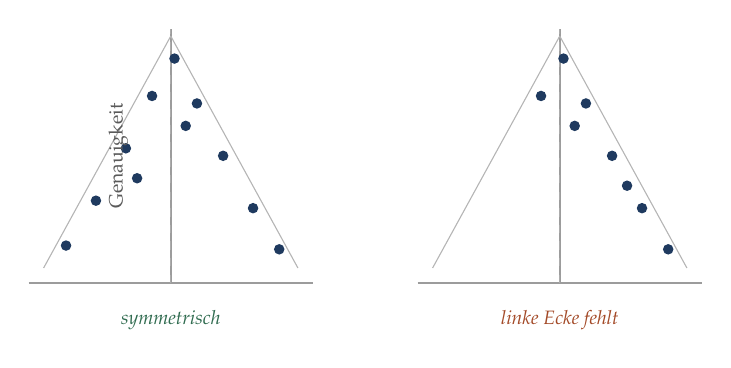
\begin{tikzpicture}[scale=0.95]
\begin{scope}
\draw[grau!60, line width=0.7pt] (0,0) -- (0,3.4);
\draw[grau!60, line width=0.7pt] (-1.9,0) -- (1.9,0);
\draw[grau!50, dashed] (0,0) -- (0,3.4);
\draw[grau!45] (0,3.3) -- (-1.7,0.2);
\draw[grau!45] (0,3.3) -- (1.7,0.2);
\foreach \x/\y in {0.05/3.0, -0.25/2.5, 0.35/2.4, -0.6/1.8, 0.7/1.7, -1.0/1.1, 1.1/1.0, -1.4/0.5, 1.45/0.45, 0.2/2.1, -0.45/1.4}
  \fill[tief] (\x,\y) circle (2.0pt);
\node[font=\scriptsize\itshape, color=gruen] at (0,-0.5) {symmetrisch};
\end{scope}
\begin{scope}[xshift=5.2cm]
\draw[grau!60, line width=0.7pt] (0,0) -- (0,3.4);
\draw[grau!60, line width=0.7pt] (-1.9,0) -- (1.9,0);
\draw[grau!50, dashed] (0,0) -- (0,3.4);
\draw[grau!45] (0,3.3) -- (-1.7,0.2);
\draw[grau!45] (0,3.3) -- (1.7,0.2);
\foreach \x/\y in {0.05/3.0, -0.25/2.5, 0.35/2.4, 0.7/1.7, 1.1/1.0, 1.45/0.45, 0.2/2.1, 0.9/1.3}
  \fill[tief] (\x,\y) circle (2.0pt);
\node[font=\scriptsize\itshape, color=akzent] at (0,-0.5) {linke Ecke fehlt};
\end{scope}
\node[font=\scriptsize, color=grau, rotate=90] at (-0.7,1.7) {Genauigkeit};
\end{tikzpicture}
\end{center}

\schritt{Die Erwartung}
Große Studien liegen oben und eng beieinander, kleine unten und weit gestreut --- ein umgekehrter Trichter, symmetrisch um den wahren Wert.

\schritt{Die Lücke}
Fehlt die untere linke Ecke, so fehlen kleine Studien mit ungünstigem Ergebnis. Genau die werden am ehesten nicht veröffentlicht.
\end{merksatz}

\begin{warnung}
\boxtitelr{Was das Trichterdiagramm nicht beweist}
\begin{center}
\renewcommand{\arraystretch}{1.5}
\begin{tabular}{@{}P{2.6cm}P{6.0cm}@{}}
\toprule
\textbf{Andere Ursachen} & Kleine Studien werden oft sorgfältiger durchgeführt oder betreffen ausgewählte Gruppen --- auch das erzeugt Unsymmetrie.\\
\textbf{Wenige Studien} & Unter zehn Studien ist die Beurteilung wertlos.\\
\textbf{Kein Beleg für Symmetrie} & Ein unauffälliger Trichter beweist nicht, dass nichts fehlt.\\
\bottomrule
\end{tabular}
\end{center}

\schritt{Die wirksame Abhilfe}
Studienregister mit Anmeldepflicht. Wer nachträglich sucht, kann Verzerrung nur vermuten; wer vorab registriert, kann sie feststellen.

\begin{center}
\begin{minipage}{0.88\textwidth}
\kursiv{Die Cochrane-Empfehlungen verlangen deshalb eine Suche in Studienregistern und, wo möglich, eine Anfrage bei den Autoren unveröffentlichter Studien. Das ist mühsam und wird unvollständig befolgt.}
\end{minipage}
\end{center}
\end{warnung}

\section{Übungsaufgaben}

\begin{aufgabe}
\boxtitel{Aufgabe 14.1 --- Drei Korrekturen anwenden}
Sechs Untergruppenanalysen liefern
\[ p = 0{,}004,\ 0{,}013,\ 0{,}029,\ 0{,}041,\ 0{,}067,\ 0{,}210 . \]
Wenden Sie Bonferroni, Holm und Benjamini-Hochberg an ($\alpha = q = 0{,}05$).

\loesung
\schritt{Schritt 1 --- Bonferroni}
Schwelle: $0{,}05/6 = 0{,}00833$.

Nur $p_{(1)} = 0{,}004$ liegt darunter. \textbf{Ein Ergebnis verworfen.}

\schritt{Schritt 2 --- Holm}
\begin{center}
{\small
\renewcommand{\arraystretch}{1.4}
\begin{tabular}{@{}P{0.8cm}P{1.4cm}P{2.0cm}P{2.0cm}@{}}
\toprule
$i$ & $p_{(i)}$ & $\alpha/(7-i)$ & \\
\midrule
$1$ & $0{,}004$ & $0{,}00833$ & \textcolor{gruen}{\checkmark}\\
$2$ & $0{,}013$ & $0{,}01000$ & \textcolor{akzent}{$\times$ Abbruch}\\
\bottomrule
\end{tabular}}
\end{center}
$0{,}013 > 0{,}010$: Abbruch. \textbf{Ein Ergebnis verworfen} --- hier leistet Holm nichts mehr als Bonferroni.

\schritt{Schritt 3 --- Benjamini-Hochberg}
\begin{center}
{\small
\renewcommand{\arraystretch}{1.4}
\begin{tabular}{@{}P{0.8cm}P{1.4cm}P{2.0cm}P{2.2cm}@{}}
\toprule
$i$ & $p_{(i)}$ & $\frac{i}{6}\cdot 0{,}05$ & $p_{(i)} \le$ Schwelle?\\
\midrule
$1$ & $0{,}004$ & $0{,}00833$ & \textcolor{gruen}{ja}\\
$2$ & $0{,}013$ & $0{,}01667$ & \textcolor{gruen}{ja}\\
$3$ & $0{,}029$ & $0{,}02500$ & \textcolor{akzent}{nein}\\
$4$ & $0{,}041$ & $0{,}03333$ & \textcolor{akzent}{nein}\\
$5$ & $0{,}067$ & $0{,}04167$ & \textcolor{akzent}{nein}\\
$6$ & $0{,}210$ & $0{,}05000$ & \textcolor{akzent}{nein}\\
\bottomrule
\end{tabular}}
\end{center}

\textbf{Achtung:} Das Verfahren sucht das \kursiv{größte} $i$, für das die Bedingung gilt --- nicht das erste Versagen. Hier ist das $i = 2$. Verworfen werden alle bis einschließlich $i=2$.

\textbf{Zwei Ergebnisse verworfen.}

\schritt{Schritt 4 --- Die Übersicht}
\begin{center}
\renewcommand{\arraystretch}{1.48}
\begin{tabular}{@{}P{3.0cm}P{2.0cm}P{2.4cm}@{}}
\toprule
\textbf{Verfahren} & \textbf{Anzahl} & \\
\midrule
ohne Korrektur & $4$ & \\
Bonferroni & $1$ & \\
Holm & $1$ & \\
Benjamini-Hochberg & $2$ & \\
\bottomrule
\end{tabular}
\end{center}

\schritt{Schritt 5 --- Die Deutung}
Ohne Korrektur wären vier Untergruppen \enquote{signifikant}. Bei sechs Tests beträgt die Wahrscheinlichkeit für mindestens einen falschen Alarm
\[ 1 - 0{,}95^6 = 0{,}265 . \]

\begin{center}
\begin{minipage}{0.86\textwidth}
\kursiv{Untergruppenanalysen sind die häufigste Quelle nicht reproduzierbarer Befunde in klinischen Studien. Der Grund ist nicht Unredlichkeit, sondern Arithmetik: Wer genug Untergruppen bildet, findet immer eine, in der die Therapie besonders gut wirkt.}
\end{minipage}
\end{center}

\schritt{Schritt 6 --- Was man stattdessen tut}
\begin{center}
\renewcommand{\arraystretch}{1.48}
\begin{tabular}{@{}P{1.0cm}P{7.4cm}@{}}
\toprule
$1$ & Untergruppen vorab benennen und begründen.\\
$2$ & Ihre Zahl klein halten.\\
$3$ & Auf \kursiv{Wechselwirkung} testen, nicht innerhalb jeder Gruppe getrennt.\\
$4$ & Befunde als erkundend kennzeichnen.\\
\bottomrule
\end{tabular}
\end{center}

Punkt $3$ ist der methodisch wichtigste: Die Frage lautet nicht \enquote{wirkt es bei Männern?}, sondern \enquote{wirkt es bei Männern \kursiv{anders} als bei Frauen?}. Das ist ein einziger Test statt zweier.
\end{aufgabe}

\begin{aufgabe}
\boxtitel{Aufgabe 14.2 --- Eine kleine Metaanalyse}
Drei Studien berichten Effekte von $2{,}0$ ($\mathrm{SE} = 1{,}0$), $4{,}0$ ($\mathrm{SE} = 0{,}5$) und $6{,}0$ ($\mathrm{SE} = 2{,}0$). Fassen Sie zusammen und beurteilen Sie die Heterogenität.

\loesung
\schritt{Schritt 1 --- Die Gewichte}
\begin{center}
\renewcommand{\arraystretch}{1.4}
\begin{tabular}{@{}P{1.4cm}P{1.4cm}P{1.4cm}P{1.6cm}P{1.6cm}@{}}
\toprule
& $\hat\theta_i$ & $\mathrm{SE}_i$ & $w_i$ & $w_i\hat\theta_i$\\
\midrule
$1$ & $2{,}0$ & $1{,}0$ & $1{,}00$ & $2{,}00$\\
$2$ & $4{,}0$ & $0{,}5$ & $\mathbf{4{,}00}$ & $16{,}00$\\
$3$ & $6{,}0$ & $2{,}0$ & $0{,}25$ & $1{,}50$\\
\midrule
& & & $\mathbf{5{,}25}$ & $\mathbf{19{,}50}$\\
\bottomrule
\end{tabular}
\end{center}

\schritt{Schritt 2 --- Der zusammengefasste Effekt}
\[ \hat\theta = \frac{19{,}50}{5{,}25} = 3{,}714 \]
\[ \mathrm{SE} = \frac{1}{\sqrt{5{,}25}} = \frac{1}{2{,}291} = 0{,}4364 \]
\[ 3{,}714 \pm 1{,}96 \cdot 0{,}4364 = 3{,}714 \pm 0{,}855 \quad\Longrightarrow\quad [\,2{,}86\ ;\ 4{,}57\,] \]

\schritt{Schritt 3 --- Die Beobachtung zu den Gewichten}
Studie 2 hat den halben Standardfehler von Studie 1 und daher das \kursiv{vierfache} Gewicht --- die Gewichte gehen mit dem Quadrat.

Studie 3 mit $\mathrm{SE} = 2{,}0$ trägt nur $0{,}25/5{,}25 = 4{,}8\,\%$ bei. Der einfache Mittelwert der drei Zahlen wäre $4{,}0$; die Gewichtung zieht ihn auf $3{,}71$.

\schritt{Schritt 4 --- Heterogenität}
\begin{center}
\renewcommand{\arraystretch}{1.4}
\begin{tabular}{@{}P{1.4cm}P{1.8cm}P{1.8cm}P{2.0cm}@{}}
\toprule
& $\hat\theta_i - \hat\theta$ & \textbf{Quadrat} & $w_i \cdot$ Quadrat\\
\midrule
$1$ & $-1{,}714$ & $2{,}938$ & $2{,}938$\\
$2$ & $0{,}286$ & $0{,}082$ & $0{,}327$\\
$3$ & $2{,}286$ & $5{,}224$ & $1{,}306$\\
\midrule
& & & $\mathbf{Q = 4{,}571}$\\
\bottomrule
\end{tabular}
\end{center}

Freiheitsgrade: $k-1 = 2$. Kritischer Wert $\chi^2_{2;\,0{,}95} = 5{,}99$.

$4{,}571 < 5{,}99$: nicht signifikant, $p = 0{,}102$.

\schritt{Schritt 5 --- $I^2$}
\[ I^2 = \frac{4{,}571 - 2}{4{,}571} = \frac{2{,}571}{4{,}571} = 0{,}563 \]

\textbf{$56\,\%$ --- erhebliche Heterogenität.}

\schritt{Schritt 6 --- Der scheinbare Widerspruch}
Der $Q$-Test ist nicht signifikant, $I^2$ zeigt erhebliche Heterogenität. Ein Widerspruch ist das nicht.

\begin{center}
\begin{minipage}{0.88\textwidth}
\kursiv{Bei drei Studien hat der $Q$-Test fast keine Macht --- er findet nur sehr grobe Unterschiede. $I^2$ misst dagegen das Ausmaß und nicht die Nachweisbarkeit. \textbf{Man richtet sich nach $I^2$, nicht nach dem $p$-Wert des $Q$-Tests} --- genau nach der Regel aus Kapitel~7, dass ein nicht signifikanter Test kein Beleg für die Nullhypothese ist.}
\end{minipage}
\end{center}

\schritt{Schritt 7 --- Was folgt}
Bei $I^2 = 56\,\%$ sollte man das zufällige Modell rechnen und vor allem nach der Ursache suchen: Warum findet Studie 1 den Wert $2{,}0$ und Studie 3 den Wert $6{,}0$? Bei drei Studien wird man das nicht klären --- und sollte das im Bericht auch sagen.
\end{aufgabe}

\begin{aufgabe}
\boxtitel{Aufgabe 14.3 --- Multiplizität aufdecken}
Eine Veröffentlichung berichtet: \enquote{Bei Frauen über $70$ mit Diabetes war die neue Therapie signifikant überlegen ($p = 0{,}03$).} Wie beurteilen Sie das?

\loesung
\schritt{Schritt 1 --- Die Fragen, die zu stellen sind}
\begin{center}
\renewcommand{\arraystretch}{1.5}
\begin{tabular}{@{}P{1.0cm}P{7.4cm}@{}}
\toprule
$1$ & War diese Untergruppe vorab festgelegt?\\
$2$ & Wie viele Untergruppen wurden geprüft?\\
$3$ & Wurde auf Wechselwirkung getestet oder nur innerhalb der Gruppe?\\
$4$ & Wie lautete das Ergebnis in der Gesamtstudie?\\
\bottomrule
\end{tabular}
\end{center}

\schritt{Schritt 2 --- Die Zahl der möglichen Untergruppen}
Die Beschreibung nennt drei Merkmale: Geschlecht, Alter, Diabetes. Bei zwei Ausprägungen je Merkmal ergeben sich
\[ 2 \cdot 2 \cdot 2 = 8 \]
Kombinationen --- und das nur, wenn keine weiteren Merkmale geprüft wurden.

Rechnet man die Einzelmerkmale und Paare hinzu:
\[ 3 \ (\text{einzeln}) + 3 \cdot 4 \ (\text{Paare}) + 8 = 23 \ \text{mögliche Untergruppen} . \]

\schritt{Schritt 3 --- Die Fehlerrate}
\[ 1 - 0{,}95^{23} = 1 - 0{,}3074 = 0{,}693 \]
In etwa sieben von zehn Fällen findet man bei $23$ Untergruppen mindestens eine mit $p < 0{,}05$ --- auch wenn die Therapie überall gleich wirkt.

\schritt{Schritt 4 --- Die Beurteilung}
\begin{center}
\begin{minipage}{0.9\textwidth}
Der Befund ist \textbf{erkundend}. Er begründet eine Hypothese für eine künftige Studie, nicht eine Behandlungsempfehlung.
\end{minipage}
\end{center}

\schritt{Schritt 5 --- Was die Formulierung verrät}
Die Angabe einer \kursiv{dreifach} eingegrenzten Untergruppe ist ein Warnzeichen. Wäre der Effekt bei Frauen vorhanden, so hätte man ihn bei Frauen berichtet. Dass drei Bedingungen nötig waren, deutet darauf hin, dass gesucht wurde, bis sich etwas fand.

\schritt{Schritt 6 --- Die sachliche Prüfung}
Es gibt einen Fall, in dem ein solcher Befund ernst zu nehmen ist: wenn er \kursiv{vorab} aus einem Wirkmechanismus abgeleitet wurde und der Wechselwirkungstest signifikant ist.

\begin{center}
\begin{minipage}{0.86\textwidth}
\kursiv{Das ist der übliche Prüfstein. Eine vorab begründete Untergruppe mit signifikanter Wechselwirkung ist ein Ergebnis; eine nachträglich gefundene ohne Wechselwirkungstest ist eine Beobachtung. Der Unterschied steht nicht in den Zahlen, sondern im Studienprotokoll --- und deshalb ist die Präregistrierung aus Kapitel~12 auch hier die eigentliche Abhilfe.}
\end{minipage}
\end{center}
\end{aufgabe}

\begin{geschichte}
\boxtitelg{Ein Name, der nicht ganz stimmt, und eine Bibliothek}
\Person{Carlo Emilio Bonferroni} (1892--1960) war Wirtschaftsmathematiker in Florenz. Die nach ihm benannte Korrektur geht auf seine Ungleichungen über Wahrscheinlichkeiten von Vereinigungen zurück --- er selbst hat sie nie auf multiples Testen angewandt.

\begin{center}
\begin{minipage}{0.9\textwidth}
\kursiv{Die Zuschreibung ist ein Beispiel für Stiglers Gesetz der Namensgebung: Keine wissenschaftliche Entdeckung ist nach ihrem Entdecker benannt. \Person{Stephen Stigler} fügte hinzu, das Gesetz sei selbst nicht von ihm --- womit es sich auf sich selbst anwendet.}
\end{minipage}
\end{center}

\schritt{Die Metaanalyse}
Den Begriff prägte \Person{Gene Glass} 1976 in einer Arbeit über die Wirksamkeit von Psychotherapie. Er fasste Hunderte von Einzelstudien zusammen, deren Ergebnisse einander zu widersprechen schienen, und kam zu einem klaren Gesamtbefund.

\schritt{Cochrane}
\Person{Archie Cochrane}, britischer Epidemiologe und ehemaliger Kriegsgefangener, forderte 1972 in einer schmalen Schrift, dass medizinische Entscheidungen auf systematisch zusammengetragenen Belegen beruhen müssten.

\begin{center}
\begin{minipage}{0.9\textwidth}
\kursiv{Er wies darauf hin, dass niemand einen Überblick über die vorhandenen randomisierten Studien habe --- nicht einmal in einzelnen Fachgebieten. Die 1993 gegründete Cochrane-Zusammenarbeit erstellt seither systematische Übersichten; sie umfasst heute über zehntausend Arbeiten und Mitwirkende in mehr als hundert Ländern.}
\end{minipage}
\end{center}
\end{geschichte}

\begin{forschung}
\boxtitelp{Wohin sich die Zusammenfassung bewegt}
\begin{center}
{\small
\renewcommand{\arraystretch}{1.45}
\begin{tabular}{@{}P{2.8cm}P{5.4cm}@{}}
\toprule
\textbf{Netzwerk-Metaanalyse} & Mehrere Therapien werden auch dann verglichen, wenn kein direkter Vergleich vorliegt --- über gemeinsame Kontrollen.\\
\textbf{Individuelle Daten} & Statt veröffentlichter Kennzahlen werden die Rohdaten der Studien zusammengeführt. Deutlich aussagekräftiger, deutlich mühsamer.\\
\textbf{Lebende Übersichten} & Die Übersicht wird fortlaufend aktualisiert, statt alle paar Jahre neu erstellt.\\
\bottomrule
\end{tabular}}
\end{center}

Die erste Zeile hat eine unangenehme Voraussetzung: Die indirekten Vergleiche gelten nur, wenn die Studien in allem übereinstimmen, was den Effekt beeinflusst. Man nennt das \Begriff{Transitivität}; sie ist nicht prüfbar, sondern muss begründet werden.

\schritt{Zur Falscherkennungsrate}
Das Verfahren von Benjamini und Hochberg stammt von 1995 und war zunächst wenig beachtet. Mit der Genomforschung änderte sich das schlagartig: Wer Zehntausende von Genen gleichzeitig prüft, kann mit der familienweisen Fehlerrate nicht arbeiten --- sie würde fast alles verwerfen.

\begin{center}
\begin{minipage}{0.88\textwidth}
\kursiv{Heute ist es das meistverwendete Multiplizitätsverfahren überhaupt. Das ist ein Beispiel dafür, wie eine neue Datenlage eine vorhandene Methode aus der Versenkung holt --- ähnlich wie der Bootstrap, der erst mit billiger Rechenzeit brauchbar wurde.}
\end{minipage}
\end{center}
\end{forschung}

\begin{merksatz}
\boxtitel{Was Sie jetzt können}
\begin{center}
\renewcommand{\arraystretch}{1.5}
\begin{tabular}{@{}P{3.2cm}P{5.4cm}@{}}
\toprule
\textbf{Multiplizität} & sechs Quellen, darunter die Verfahrenswahl\\
\textbf{Bonferroni, Holm, BH} & eins, zwei, fünf bei denselben Daten\\
\textbf{Metaanalyse} & Gewichtung mit $1/\mathrm{SE}^2$\\
\textbf{$Q$ und $I^2$} & und warum man sich nach $I^2$ richtet\\
\textbf{Trichterdiagramm} & und was es nicht beweist\\
\bottomrule
\end{tabular}
\end{center}

\begin{center}
\begin{minipage}{0.88\textwidth}
\kursiv{Damit endet Teil~V. Das letzte Kapitel berichtet, worüber in der Statistik heute gestritten wird --- und vieles davon hat seinen Ursprung in den Rechnungen dieses Kapitels.}
\end{minipage}
\end{center}
\end{merksatz}

\part{Aktueller Stand}

\chapter{Wo die Statistik heute steht}

\section{Die Replikationskrise}

\begin{merksatz}
\boxtitel{Der Befund}
Seit etwa 2011 haben mehrere groß angelegte Wiederholungsvorhaben versucht, veröffentlichte Ergebnisse nachzuvollziehen.

\begin{center}
{\small
\renewcommand{\arraystretch}{1.48}
\begin{tabular}{@{}P{2.6cm}P{2.4cm}P{3.0cm}@{}}
\toprule
\textbf{Gebiet} & \textbf{Wiederholt} & \textbf{Bestätigt}\\
\midrule
Psychologie & $100$ Studien & etwa $36\,\%$\\
Krebsbiologie & $50$ Vorhaben & etwa die Hälfte, mit kleineren Effekten\\
Wirtschaft & $18$ Studien & etwa $61\,\%$\\
\bottomrule
\end{tabular}}
\end{center}

\begin{center}
\begin{minipage}{0.88\textwidth}
\kursiv{Die Zahlen sind umstritten --- was als \enquote{bestätigt} gilt, ist selbst eine Entscheidung. Unstrittig ist, dass die Anteile weit unter dem liegen, was man erwarten würde, wenn die ursprünglichen Befunde überwiegend zuträfen.}
\end{minipage}
\end{center}
\end{merksatz}

\begin{merksatz}
\boxtitel{Die Rechnung, die das erklärt}
Aufgabe 7.3 hat sie bereits vorgeführt. Hier noch einmal allgemein.

Sei $\pi_0$ der Anteil der geprüften Hypothesen, die zutreffen; $\alpha$ das Niveau, $1-\beta$ die Macht. Dann gilt unter den signifikanten Ergebnissen:
\[ \Pr[\text{falsch} \mid \text{signifikant}] = \frac{(1-\pi_0)\,\alpha}{(1-\pi_0)\,\alpha + \pi_0\,(1-\beta)} . \]

\begin{center}
{\small
\renewcommand{\arraystretch}{1.48}
\begin{tabular}{@{}P{1.8cm}P{1.8cm}P{2.4cm}P{2.0cm}@{}}
\toprule
$\pi_0$ & \textbf{Macht} & \textbf{falsch positiv} & \\
\midrule
$0{,}50$ & $0{,}80$ & $5{,}9\,\%$ & \textcolor{gruen}{gut}\\
$0{,}10$ & $0{,}80$ & $36{,}0\,\%$ & \\
$0{,}10$ & $0{,}40$ & $52{,}9\,\%$ & \textcolor{akzent}{Mehrheit falsch}\\
$0{,}05$ & $0{,}40$ & \textcolor{akzent}{$\mathbf{70{,}4\,\%}$} & \\
\bottomrule
\end{tabular}}
\end{center}

\begin{center}
\begin{minipage}{0.9\textwidth}
\textbf{Zwei Größen bestimmen das Ergebnis: wie plausibel die geprüften Hypothesen waren, und wie groß die Studien sind.} Beide kommen im $p$-Wert nicht vor.
\end{minipage}
\end{center}

\begin{center}
\begin{minipage}{0.88\textwidth}
\kursiv{\Person{John Ioannidis} führte diese Rechnung 2005 in einem Aufsatz mit dem Titel \kursiv{Why Most Published Research Findings Are False} vor. Der Titel war absichtlich zugespitzt; die Rechnung ist elementar und unbestritten.}
\end{minipage}
\end{center}
\end{merksatz}

\begin{warnung}
\boxtitelr{Die Freiheitsgrade des Auswertenden}
Zur Rechnung kommt ein zweiter Umstand hinzu. Zwischen Daten und Ergebnis liegen Dutzende von Entscheidungen:

\begin{center}
{\small
\renewcommand{\arraystretch}{1.48}
\begin{tabular}{@{}P{2.4cm}P{6.2cm}@{}}
\toprule
Ausreißer & ausschließen oder behalten, nach welcher Regel?\\
Umformung & logarithmieren oder nicht?\\
Kovariablen & welche adjustieren?\\
Untergruppen & welche berichten?\\
Verfahren & $t$-Test oder Rangtest?\\
Endpunkt & welcher ist der primäre?\\
Fallzahl & wann aufhören zu erheben?\\
\bottomrule
\end{tabular}}
\end{center}

\begin{center}
\begin{minipage}{0.9\textwidth}
Jede dieser Entscheidungen ist für sich vertretbar. Trifft man sie aber \kursiv{nach} dem Blick auf die Daten, so entsteht eine verborgene Multiplizität --- ohne dass jemand bewusst manipuliert.
\end{minipage}
\end{center}

\schritt{Die Größenordnung}
Simulationsstudien zeigen: Bei mäßiger Ausnutzung dieser Freiheitsgrade steigt die tatsächliche Fehlerrate erster Art von fünf auf über sechzig Prozent.

\begin{center}
\begin{minipage}{0.88\textwidth}
\kursiv{\Person{Andrew Gelman} nennt das den \kursiv{Garten der sich gabelnden Pfade}: Man muss nicht viele Analysen durchführen und die beste wählen --- es genügt, dass man bei anderen Daten eine andere Analyse gewählt hätte. Der $p$-Wert der einen tatsächlich durchgeführten Analyse ist dann trotzdem ungültig.}
\end{minipage}
\end{center}
\end{warnung}

\section{Die Debatte um den $p$-Wert}

\begin{merksatz}
\boxtitel{Die Lager}
\begin{center}
{\small
\renewcommand{\arraystretch}{1.52}
\begin{tabular}{@{}P{2.4cm}P{6.2cm}@{}}
\toprule
\textbf{Schwelle senken} & $p < 0{,}005$ für neue Befunde. Einfach umzusetzen, vervierfacht aber die nötigen Fallzahlen.\\
\textbf{Aufgeben} & Das Wort \enquote{signifikant} streichen, Intervalle berichten. Über achthundert Unterzeichner 2019.\\
\textbf{Bayessch} & Bayes-Faktoren statt $p$-Werten. Löst das Deutungsproblem, schafft das Priori-Problem.\\
\textbf{Beibehalten} & Der $p$-Wert ist nicht das Problem, sondern sein Gebrauch als Schwelle.\\
\bottomrule
\end{tabular}}
\end{center}

\begin{center}
\begin{minipage}{0.88\textwidth}
\kursiv{Die vierte Zeile hat gute Argumente: Jede Schwelle, gleich wo sie liegt, erzeugt dieselben Anreize. Wer $0{,}005$ fordert, verschiebt das Problem, statt es zu lösen --- und macht Studien so teuer, dass weniger Fragen untersucht werden.}
\end{minipage}
\end{center}
\end{merksatz}

\begin{merksatz}
\boxtitel{Was sich tatsächlich geändert hat}
Unabhängig vom Ausgang der Debatte hat sich die Berichtspraxis verschoben.

\begin{center}
{\small
\renewcommand{\arraystretch}{1.5}
\begin{tabular}{@{}P{2.6cm}P{6.0cm}@{}}
\toprule
\textbf{Effektschätzer} & Mit Intervall, in der Einheit der Sache --- in guten Zeitschriften Pflicht.\\
\textbf{Präregistrierung} & Seit 2005 für klinische Studien vorgeschrieben, zunehmend auch in anderen Fächern.\\
\textbf{Daten und Code} & Offenlegung wird zunehmend verlangt.\\
\textbf{Registered Reports} & Die Zeitschrift nimmt die Arbeit an, \kursiv{bevor} die Daten erhoben sind --- allein aufgrund der Fragestellung und des Plans.\\
\bottomrule
\end{tabular}}
\end{center}

\begin{center}
\begin{minipage}{0.88\textwidth}
\kursiv{Die letzte Zeile ist der wirksamste der vier Vorschläge, weil sie an der Ursache ansetzt: Wenn die Annahme nicht vom Ergebnis abhängt, verschwindet sowohl der Anreiz zur Suche nach Signifikanz als auch die Publikationsverzerrung. Untersuchungen an solchen Arbeiten finden deutlich niedrigere Anteile positiver Ergebnisse --- etwa vierzig Prozent statt über neunzig.}
\end{minipage}
\end{center}
\end{merksatz}

\section{Kausale Inferenz}

\begin{merksatz}
\boxtitel{Ein Gebiet, das es vor dreißig Jahren nicht gab}
Kapitel~3 endete mit der Feststellung, dass die Korrelation die vier Erklärungen nicht unterscheiden kann. Kapitel~12 nannte die Randomisierung als Ausweg. Was, wenn man nicht randomisieren kann?

\begin{center}
\begin{minipage}{0.9\textwidth}
Die moderne Antwort lautet: Man schreibt die vermuteten Wirkungszusammenhänge als Graphen auf und leitet daraus ab, was aus den Daten schätzbar ist und was nicht.
\end{minipage}
\end{center}

\begin{center}
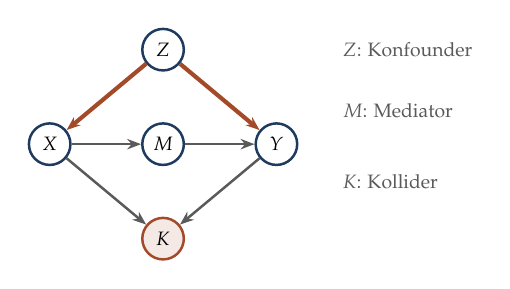
\begin{tikzpicture}[scale=1.2]
\node[knotenb] (z) at (0,1.0) {$Z$};
\node[knotenb] (x) at (-1.2,0) {$X$};
\node[knotenb] (m) at (0,0) {$M$};
\node[knotenb] (y) at (1.2,0) {$Y$};
\node[knotenr] (k) at (0,-1.0) {$K$};
\draw[kanted, -{Stealth[length=5pt]}] (z) -- (x);
\draw[kanted, -{Stealth[length=5pt]}] (z) -- (y);
\draw[kante, -{Stealth[length=5pt]}] (x) -- (m);
\draw[kante, -{Stealth[length=5pt]}] (m) -- (y);
\draw[kante, -{Stealth[length=5pt]}] (x) -- (k);
\draw[kante, -{Stealth[length=5pt]}] (y) -- (k);
\node[font=\scriptsize, color=grau, anchor=west] at (1.8,1.0) {$Z$: Konfounder};
\node[font=\scriptsize, color=grau, anchor=west] at (1.8,0.35) {$M$: Mediator};
\node[font=\scriptsize, color=grau, anchor=west] at (1.8,-0.4) {$K$: Kollider};
\end{tikzpicture}
\end{center}

\schritt{Was der Graph entscheidet}
\begin{center}
\renewcommand{\arraystretch}{1.48}
\begin{tabular}{@{}P{2.0cm}P{2.4cm}P{3.4cm}@{}}
\toprule
\textbf{Größe} & \textbf{Adjustieren?} & \textbf{Sonst}\\
\midrule
$Z$ & \textcolor{gruen}{ja} & verzerrter Effekt\\
$M$ & \textcolor{akzent}{nein} & Effekt verschwindet\\
$K$ & \textcolor{akzent}{nein} & \textcolor{akzent}{Scheineffekt entsteht}\\
\bottomrule
\end{tabular}
\end{center}

\begin{center}
\begin{minipage}{0.88\textwidth}
\kursiv{Die dritte Zeile bleibt der überraschendste Befund des Gebiets: Das Hinzunehmen einer weiteren Größe kann einen Zusammenhang \kursiv{erzeugen}. Damit ist die verbreitete Vorstellung widerlegt, mehr Kontrollvariablen seien stets besser.}
\end{minipage}
\end{center}
\end{merksatz}

\begin{merksatz}
\boxtitel{Die Werkzeuge}
\begin{center}
{\small
\renewcommand{\arraystretch}{1.5}
\begin{tabular}{@{}P{3.2cm}P{5.4cm}@{}}
\toprule
\textbf{Gerichtete Graphen} & Machen die Annahmen sichtbar und prüfbar --- man sieht, was man voraussetzt.\\
\textbf{Propensity Score} & Personen werden nach ihrer geschätzten Behandlungswahrscheinlichkeit zusammengeführt.\\
\textbf{Instrument\-variablen} & Eine Größe, die nur über die Behandlung wirkt, ersetzt die Randomisierung teilweise.\\
\textbf{Zielstudie} & Man entwirft die randomisierte Studie, die man gerne hätte, und bildet sie in Beobachtungsdaten nach.\\
\bottomrule
\end{tabular}}
\end{center}

\begin{center}
\begin{minipage}{0.88\textwidth}
\kursiv{Die letzte Zeile hat sich als besonders fruchtbar erwiesen. Viele Widersprüche zwischen Beobachtungsstudien und späteren randomisierten Studien ließen sich nachträglich darauf zurückführen, dass die Beobachtungsstudie eine andere Frage beantwortet hatte --- etwa durch den unsterblichen Zeitraum aus Kapitel~12.}
\end{minipage}
\end{center}
\end{merksatz}

\section{Statistik und maschinelles Lernen}

\begin{merksatz}
\boxtitel{Zwei Kulturen}
\begin{center}
{\small
\renewcommand{\arraystretch}{1.52}
\begin{tabular}{@{}P{2.0cm}P{3.2cm}P{3.0cm}@{}}
\toprule
& \textbf{Statistik} & \textbf{Maschinelles Lernen}\\
\midrule
Ziel & Verstehen, schätzen & Vorhersagen\\
Modell & möglichst einfach & beliebig komplex\\
Prüfung & Voraussetzungen & Leistung an neuen Daten\\
Frage & Warum? & Wie gut?\\
\bottomrule
\end{tabular}}
\end{center}

\begin{center}
\begin{minipage}{0.88\textwidth}
\kursiv{\Person{Leo Breiman} beschrieb diesen Gegensatz 2001 in einem viel diskutierten Aufsatz. Er warf der Statistik vor, sich zu sehr an Modelle zu klammern, die sie für wahr halte, statt die Vorhersageleistung zu prüfen. Der Vorwurf saß und hat die Statistik verändert.}
\end{minipage}
\end{center}
\end{merksatz}

\begin{warnung}
\boxtitelr{Was Vorhersage nicht ersetzt}
\begin{center}
\renewcommand{\arraystretch}{1.5}
\begin{tabular}{@{}P{3.0cm}P{5.6cm}@{}}
\toprule
\textbf{Kausalität} & Ein Modell, das gut vorhersagt, sagt nichts darüber, was geschähe, wenn man eingreift.\\
\textbf{Übertrag\-barkeit} & Ändert sich die Umgebung, so versagt ein Modell, das auf Begleitumständen beruht.\\
\textbf{Die Prävalenz} & Die Rechnung aus Kapitel~13 gilt unverändert --- auch für das beste System.\\
\bottomrule
\end{tabular}
\end{center}

\schritt{Ein lehrreiches Beispiel}
Ein System zur Vorhersage des Sterberisikos bei Lungenentzündung stufte Personen mit Asthma als \kursiv{weniger} gefährdet ein --- weil sie in den Trainingsdaten seltener starben.

Der Grund: Sie wurden sofort auf die Intensivstation aufgenommen. Das Modell hatte die Behandlung gelernt, nicht das Risiko.

\begin{center}
\begin{minipage}{0.88\textwidth}
\kursiv{Hätte man danach gehandelt, wären genau diese Personen weniger überwacht worden. Das ist kein Fehler der Methode, sondern eine Verwechslung der Frage: Das Modell beantwortete \enquote{wer stirbt?} und wurde gelesen als \enquote{wer braucht Überwachung?}.}
\end{minipage}
\end{center}
\end{warnung}

\section{Eine Bilanz}

\begin{merksatz}
\boxtitel{Was geklärt ist und was nicht}
\begin{center}
{\small
\renewcommand{\arraystretch}{1.45}
\begin{tabular}{@{}P{3.4cm}P{2.2cm}P{2.6cm}@{}}
\toprule
\textbf{Frage} & \textbf{Kapitel} & \textbf{Stand}\\
\midrule
Was ist ein $p$-Wert? & $7$ & \textcolor{gruen}{geklärt}\\
Soll man ihn benutzen? & $7$, $15$ & \textcolor{akzent}{\textbf{strittig}}\\
Wie schätzt man? & $5$ & \textcolor{gruen}{geklärt}\\
Welcher Schätzer ist der beste? & $5$ & \textcolor{mittel}{hängt vom Ziel ab}\\
Welche Tests wann? & $8$, $9$ & \textcolor{gruen}{weitgehend geklärt}\\
Wann korrigieren? & $14$ & \textcolor{akzent}{strittig}\\
Klassisch oder bayessch? & $5$, $15$ & \textcolor{akzent}{\textbf{seit 1930 offen}}\\
Kausalität ohne Randomisierung? & $12$, $15$ & \textcolor{mittel}{in Bewegung}\\
\bottomrule
\end{tabular}}
\end{center}

\begin{center}
\begin{minipage}{0.88\textwidth}
\kursiv{Auffällig ist das Muster: Die \kursiv{Rechnungen} sind geklärt, die \kursiv{Entscheidungen} nicht. Das ist genau die Zweiteilung aus dem Vorwort --- und sie ist keine vorübergehende Unordnung, sondern die Eigenart des Gebiets.}
\end{minipage}
\end{center}
\end{merksatz}

\begin{merksatz}
\boxtitel{Sechs Sätze, die bleiben}
\begin{center}
{\small
\renewcommand{\arraystretch}{1.55}
\begin{tabular}{@{}P{0.7cm}P{7.7cm}@{}}
\toprule
$1$ & Der $p$-Wert ist $\Pr[\text{Daten} \mid H_0]$, nicht $\Pr[H_0 \mid \text{Daten}]$. Alle sieben Fehldeutungen folgen aus dieser Verwechslung.\\
$2$ & Ein Konfidenzintervall ist eine Aussage über das Verfahren, nicht über das einzelne Intervall.\\
$3$ & Signifikanz ist nicht Bedeutsamkeit; nicht signifikant ist nicht \enquote{kein Unterschied}.\\
$4$ & Der prädiktive Wert hängt von der Prävalenz ab, Sensitivität und Spezifität nicht.\\
$5$ & Kein Rechenverfahren repariert, was bei der Erhebung falsch gemacht wurde.\\
$6$ & Wer nach dem Blick auf die Daten entscheidet, wie er rechnet, hat kein Ergebnis, sondern eine Hypothese.\\
\bottomrule
\end{tabular}}
\end{center}
\end{merksatz}

\begin{merksatz}
\boxtitel{Ein Schlusswort}
\begin{center}
\begin{minipage}{0.9\textwidth}
Dieser Band begann mit zwei Befunden: dass der $p$-Wert und das Konfidenzintervall mehrheitlich falsch gedeutet werden. Er endet bei einer Debatte darüber, ob man beide überhaupt weiter verwenden soll.

Dazwischen liegen fünfzehn Kapitel, in denen jede Formel hergeleitet, jede Voraussetzung benannt und zu jedem Verfahren der Bruchfall gezeigt wurde. Das war die Absicht: nicht, Rechenwege zu vermitteln --- die stehen in jedem Programm ---, sondern die Frage zu schärfen, wann ein Verfahren überhaupt anwendbar ist.

Wenn Sie von nun an bei jedem Ergebnis zuerst nach dem Konfidenzintervall suchen, bei jedem Chancenverhältnis nach der Häufigkeit des Ereignisses, bei jedem positiven Befund nach der Prävalenz und bei jeder Untergruppe nach dem Studienprotokoll --- dann hat der Band mehr geleistet, als jede Formel es könnte.
\end{minipage}
\end{center}

\begin{center}
\begin{minipage}{0.88\textwidth}
\kursiv{Die Statistik ist nicht schwierig, weil ihre Mathematik schwierig wäre. Sie ist schwierig, weil sie in jedem Einzelfall verlangt, dass jemand urteilt --- und weil die Rechnung dieses Urteil nicht ersetzen kann, sondern nur voraussetzt.}
\end{minipage}
\end{center}
\end{merksatz}

\appendix
\part{Anhang}

\newcommand{\lit}[3]{\vspace{5pt}\noindent\textbf{[#1]} #2\par\nopagebreak\vspace{1pt}{\small\itshape\color{grau} #3}\par\vspace{2pt}}

\chapter{Formelsammlung und Übersicht}

\section{Beschreiben}

\begin{merksatz}
\boxtitel{Lage und Streuung}
\begin{center}
{\small
\renewcommand{\arraystretch}{1.6}
\begin{tabular}{@{}P{4.4cm}P{4.2cm}@{}}
\toprule
$\MW = \frac{1}{n}\sum_i x_i$ & arithmetisches Mittel (2.2)\\
$\sum_i (x_i-\MW) = 0$ & Satz 2.3\\
$\sum(x_i-a)^2$ minimal bei $a=\MW$ & Satz 2.4\\
$\sum|x_i-a|$ minimal bei $a=\Med$ & Satz 2.6\\
$s^2 = \frac{1}{n-1}\sum (x_i-\MW)^2$ & Stichprobenvarianz\\
$\sum(x_i-\MW)^2 = \sum x_i^2 - n\MW^2$ & Verschiebungssatz (2.11)\\
$\mathrm{IQR} = Q_3 - Q_1$ & Quartilsabstand\\
$v = s/\MW$ & Variationskoeffizient\\
$z_i = (x_i-\MW)/s$ & Standardisierung\\
\bottomrule
\end{tabular}}
\end{center}
\end{merksatz}

\begin{merksatz}
\boxtitel{Zusammenhang}
\begin{center}
{\small
\renewcommand{\arraystretch}{1.6}
\begin{tabular}{@{}P{4.4cm}P{4.2cm}@{}}
\toprule
$s_{xy} = \frac{1}{n-1}\sum(x_i-\MW)(y_i-\overline y)$ & Kovarianz (3.1)\\
$\sum(x-\MW)(y-\overline y) = \sum xy - n\MW\overline y$ & Satz 3.2\\
$r = s_{xy}/(s_xs_y)$ & Korrelation (3.3)\\
$-1 \le r \le 1$ & Satz 3.4\\
$r_s = 1 - \frac{6\sum d_i^2}{n(n^2-1)}$ & Spearman, ohne Bindungen\\
\bottomrule
\end{tabular}}
\end{center}
\end{merksatz}

\section{Schätzen und Testen}

\begin{merksatz}
\boxtitel{Grundlagen}
\begin{center}
{\small
\renewcommand{\arraystretch}{1.6}
\begin{tabular}{@{}P{4.4cm}P{4.2cm}@{}}
\toprule
$\mathbb{E}[\overline X] = \mu$ & Satz 4.4\\
$\Var[\overline X] = \sigma^2/n$ & Satz 4.4, braucht Unabhängigkeit\\
$\mathrm{SE} = s/\sqrt n$ & Standardfehler (4.5)\\
$\mathbb{E}[X^2] = \Var[X] + \mu^2$ & Hilfssatz zu 5.3\\
$\mathbb{E}[S^2] = \sigma^2$ & Satz 5.3 --- das $n-1$\\
$\mathrm{MSE} = \Var + \mathrm{Bias}^2$ & Satz 5.6\\
$\hat\pi = k/n$ & ML für den Anteil\\
$\hat\mu = \MW$, $\hat\sigma^2 = \frac1n\sum(x-\MW)^2$ & ML, normal --- verzerrt\\
$\hat\lambda = 1/\MW$ & ML, exponentiell\\
\bottomrule
\end{tabular}}
\end{center}
\end{merksatz}

\begin{merksatz}
\boxtitel{Intervalle und Tests}
\begin{center}
{\small
\renewcommand{\arraystretch}{1.6}
\begin{tabular}{@{}P{4.4cm}P{4.2cm}@{}}
\toprule
$\MW \pm t_{n-1}\,\frac{s}{\sqrt n}$ & $t$-Intervall (6.2)\\
$s_p^2 = \frac{(n_A-1)s_A^2+(n_B-1)s_B^2}{n_A+n_B-2}$ & gepoolte Varianz\\
$\mathrm{SE} = s_p\sqrt{\frac{1}{n_A}+\frac{1}{n_B}}$ & Student\\
$\mathrm{SE} = \sqrt{\frac{s_A^2}{n_A}+\frac{s_B^2}{n_B}}$ & Welch\\
Wilson & statt Wald bei Anteilen\\
$3/n$ & Dreierregel bei null Ereignissen\\
$n = \frac{2(z_{1-\alpha/2}+z_{1-\beta})^2\sigma^2}{\delta^2}$ & Fallzahl je Gruppe\\
$\chi^2 = \sum \frac{(O-E)^2}{E}$ & Vierfeldertafel\\
$U_A = R_A - \frac{n_A(n_A+1)}{2}$ & Mann-Whitney\\
\bottomrule
\end{tabular}}
\end{center}
\end{merksatz}

\section{Modelle und Medizin}

\begin{merksatz}
\boxtitel{Regression}
\begin{center}
{\small
\renewcommand{\arraystretch}{1.6}
\begin{tabular}{@{}P{4.4cm}P{4.2cm}@{}}
\toprule
$b = \frac{\sum(x-\MW)(y-\overline y)}{\sum(x-\MW)^2}$ & Satz 10.2\\
$a = \overline y - b\MW$ & Gerade durch den Schwerpunkt\\
$b = r\,s_y/s_x$ & Zusammenhang mit $r$\\
$R^2 = r^2$ & nur bei einfacher Regression\\
$\widehat{\mathrm{SE}}(b) = s_e/\sqrt{\sum(x-\MW)^2}$ & mit $s_e^2 = SS_{\text{Rest}}/(n-2)$\\
$\hat z_y = r\,z_x$ & Regression zur Mitte\\
\bottomrule
\end{tabular}}
\end{center}
\end{merksatz}

\begin{merksatz}
\boxtitel{Andere Zielgrößen und Diagnostik}
\begin{center}
{\small
\renewcommand{\arraystretch}{1.6}
\begin{tabular}{@{}P{4.4cm}P{4.2cm}@{}}
\toprule
$\operatorname{logit}(\pi) = \ln\frac{\pi}{1-\pi}$ & logistisches Modell (11.2)\\
$e^{\beta}$ & Chancenverhältnis je Einheit\\
$\mathrm{OR} = \frac{ad}{bc}$ & Kreuzprodukt\\
$\widehat{\mathrm{SE}}(\ln\mathrm{OR}) = \sqrt{\frac1a+\frac1b+\frac1c+\frac1d}$ & \\
$S(t) = \prod_{t_j \le t}(1-d_j/n_j)$ & Kaplan-Meier\\
$h(t\mid x) = h_0(t)e^{\beta x}$ & Cox (11.3)\\
$\mathrm{LQ}^{+} = \frac{\text{Sens}}{1-\text{Spez}}$ & Likelihood-Quotient\\
Chance nachher $=$ Chance vorher $\times\ \mathrm{LQ}$ & Bayes, Chancenform\\
$\mathrm{AUC} = U/(n_1n_2)$ & wie Mann-Whitney\\
\bottomrule
\end{tabular}}
\end{center}
\end{merksatz}

\begin{merksatz}
\boxtitel{Viele Tests, viele Studien}
\begin{center}
{\small
\renewcommand{\arraystretch}{1.6}
\begin{tabular}{@{}P{4.4cm}P{4.2cm}@{}}
\toprule
$1-(1-\alpha)^m$ & Fehlerrate bei $m$ Tests\\
$\alpha/m$ & Bonferroni\\
$\alpha/(m-i+1)$ & Holm, aufsteigend\\
$\frac{i}{m}q$ & Benjamini-Hochberg\\
$w_i = 1/\mathrm{SE}_i^2$ & Metaanalyse, fester Effekt\\
$Q = \sum w_i(\hat\theta_i - \hat\theta)^2$ & Heterogenität\\
$I^2 = \max(0, \frac{Q-(k-1)}{Q})$ & \\
$w_i^{*} = 1/(\mathrm{SE}_i^2+\tau^2)$ & zufälliger Effekt\\
\bottomrule
\end{tabular}}
\end{center}
\end{merksatz}

\section{Die Landkarte des Bandes}

\begin{merksatz}
\boxtitel{Welcher Satz wo --- und worauf er beruht}
\begin{center}
{\small
\renewcommand{\arraystretch}{1.42}
\begin{tabular}{@{}P{3.4cm}P{1.2cm}P{3.6cm}@{}}
\toprule
\textbf{Ergebnis} & \textbf{Kap.} & \textbf{Beruht auf}\\
\midrule
Skalenniveaus & $1$ & erlaubte Umformungen\\
Mittelwert minimiert Quadrate & $2$ & Null einfügen\\
Median minimiert Beträge & $2$ & Verschiebeargument\\
Verschiebungssatz & $2$ & Ausquadrieren\\
$-1 \le r \le 1$ & $3$ & Summe von Quadraten\\
Simpson & $3$ & gewichtetes Mittel\\
$\Var[\overline X] = \sigma^2/n$ & $4$ & Unabhängigkeit\\
Grenzwertsatz & $4$ & \textcolor{grau}{nicht bewiesen}\\
$\mathbb{E}[S^2] = \sigma^2$ & $5$ & Satz 4.4 auf $\overline X$\\
MSE-Zerlegung & $5$ & derselbe Kniff wie 2.4\\
ML für $\mu$ & $5$ & \textbf{Satz 2.4}\\
$t$-Intervall & $6$ & Umformung der Ungleichung\\
Überlappungs\-problem & $6$ & $\sqrt{a^2+b^2} < a+b$\\
Sieben Fehldeutungen & $7$ & $\Pr[D|H_0]$ gegen $\Pr[H_0|D]$\\
Varianzanalyse & $8$ & Zerlegung wie 2.4\\
Fisher exakt & $8$ & Abzählen\\
Permutationstest & $9$ & Austauschbarkeit\\
Kleinste Quadrate & $10$ & Ableiten, Satz 2.3\\
Regression zur Mitte & $10$ & $b = rs_y/s_x$\\
Chancenverhältnis & $11$ & Logit-Differenz\\
Kaplan-Meier & $11$ & Produkt bedingter Anteile\\
Fall-Kontroll & $12$ & Spaltenweise Bildung\\
Prävalenz\-abhängigkeit & $13$ & Satz von Bayes\\
AUC $= U/(n_1n_2)$ & $13$ & Kapitel~9\\
Bonferroni & $14$ & Vereinigungs\-abschätzung\\
\bottomrule
\end{tabular}}
\end{center}
\end{merksatz}

\begin{merksatz}
\boxtitel{Was in diesem Band \kursiv{nicht} bewiesen wurde}
\begin{center}
{\small
\renewcommand{\arraystretch}{1.5}
\begin{tabular}{@{}P{3.4cm}P{1.4cm}P{3.4cm}@{}}
\toprule
\textbf{Ergebnis} & \textbf{Kap.} & \textbf{Wo es steht}\\
\midrule
Zentraler Grenzwertsatz & $4$ & Band 4, Teil IV\\
Form der $t$-Verteilung & $6$ & Casella/Berger\zit{7}\\
Zweite Momentenmethode & $9$ & Efron/Tibshirani\zit{11}\\
Partielle Likelihood & $11$ & Cox\zit{9}\\
Tschebyschew-Ungleichung & $5$ & Band 4, Kapitel 7\\
\bottomrule
\end{tabular}}
\end{center}

\begin{center}
\begin{minipage}{0.88\textwidth}
\kursiv{Fünf Auslassungen. Jede ist im Text als solche benannt, mit Begründung und Fundstelle. Das ist die einzige zulässige Form, die Regel dieses Werkes zu brechen: offen und mit Quellenangabe.}
\end{minipage}
\end{center}
\end{merksatz}

\section{Zeittafel}

\begin{merksatz}
\boxtitel{Von den Zitronen bis zur Replikationskrise}
\begin{center}
{\small
\renewcommand{\arraystretch}{1.36}
\begin{tabular}{@{}P{1.4cm}P{2.8cm}P{4.0cm}@{}}
\toprule
\textbf{Jahr} & \textbf{Person} & \textbf{Ereignis}\\
\midrule
$1747$ & Lind & erster kontrollierter Versuch\\
$1763$ & Bayes & Satz über umgekehrte Wahrscheinlichkeit\\
$1774$ & Laplace & allgemeine Form\\
$1805$ & Legendre & kleinste Quadrate\\
$1809$ & Gauß & Normalverteilung als Fehlergesetz\\
$1835$ & Quetelet & der Durchschnittsmensch\\
$1858$ & Nightingale & Statistik als Argument\\
$1886$ & Galton & Regression zur Mitte\\
$1896$ & Pearson & Korrelationskoeffizient\\
$1900$ & Pearson & $\chi^2$-Test\\
$1908$ & Gosset & $t$-Verteilung\\
$1922$ & Fisher & Maximum-Likelihood\\
$1925$ & Fisher & Signifikanztest, Varianzanalyse\\
$1928$ & Neyman, Pearson & Entscheidungsverfahren\\
$1935$ & Fisher & \kursiv{Design of Experiments}\\
$1937$ & Neyman & Konfidenzintervall\\
$1945$ & Wilcoxon & Rangtests\\
$1946$ & Stevens & Skalenniveaus\\
$1947$ & Mann, Whitney & $U$-Test\\
$1948$ & Bradford Hill & erste randomisierte Studie\\
$1956$ & Stein & Zusammenziehen\\
$1958$ & Kaplan, Meier & Überlebenskurve\\
$1965$ & Bradford Hill & neun Kriterien\\
$1972$ & Cox & Regressionsmodell\\
$1972$ & Cochrane & \kursiv{Effectiveness and Efficiency}\\
$1976$ & Glass & Metaanalyse\\
$1977$ & Tukey & \kursiv{Exploratory Data Analysis}\\
$1979$ & Efron & Bootstrap\\
$1993$ & --- & Cochrane-Zusammenarbeit\\
$1995$ & Benjamini, Hochberg & Falscherkennungsrate\\
$2001$ & Breiman & die zwei Kulturen\\
$2005$ & Ioannidis & \kursiv{Most findings are false}\\
$2005$ & --- & Registrierungspflicht\\
$2009$ & Pearl & \kursiv{Causality}, 2.\ Auflage\\
$2015$ & Open Science & Wiederholungsvorhaben\\
$2016$ & ASA & Erklärung zum $p$-Wert\\
$2019$ & Amrhein u.\,a. & \enquote{signifikant} abschaffen\\
\bottomrule
\end{tabular}}
\end{center}
\end{merksatz}

\section{Glossar}

\begin{merksatz}
\boxtitel{Begriffe von A bis Z}
\begin{center}
{\small
\renewcommand{\arraystretch}{1.3}
\begin{longtable}{@{}P{3.2cm}P{5.4cm}@{}}
\toprule
\textbf{Begriff} & \textbf{Bedeutung}\\
\midrule
\endhead
Alpha & vorab festgelegtes Niveau (7.3)\\
AUC & Fläche unter der ROC-Kurve (13.2)\\
Ausreißer & auffällig abweichender Wert (2.4)\\
Austauschbarkeit & Voraussetzung des Permutationstests (9)\\
Bias & systematische Abweichung (5.2)\\
Bootstrap & Ziehen aus der Stichprobe (9)\\
Bruchpunkt & Robustheitsmaß (2.9)\\
Chance & $\pi/(1-\pi)$ (11.1)\\
Erwartungstreu & $\mathbb{E}[\hat\theta] = \theta$ (5.2)\\
Fallzahl & Umfang je Gruppe (7)\\
Freiheitsgrade & Zahl unabhängiger Abweichungen\\
Hazard & momentane Ereignisrate (11.3)\\
Heterogenität & echte Verschiedenheit der Studien (14)\\
$I^2$ & Anteil nicht zufälliger Streuung (14)\\
Intention-to-treat & Auswertung wie randomisiert (12)\\
Kollider & von beiden beeinflusst (3, 15)\\
Konfidenzintervall & Überdeckung des Verfahrens (6.1)\\
Konfounder & wirkt auf Ursache und Wirkung (3)\\
Konsistenz & Annäherung bei wachsendem $n$ (5.4)\\
Kovarianz & ungenormtes Zusammenhangsmaß (3.1)\\
Likelihood & Wahrscheinlichkeit der Daten als Funktion von $\theta$ (5)\\
Macht & $1-\beta$ (7.3)\\
Median & mittlere Ausprägung (2.5)\\
Mediator & liegt auf dem Wirkungsweg (3)\\
Metaanalyse & Zusammenfassung mehrerer Studien (14)\\
Multiplizität & viele Tests zugleich (14)\\
Nullhypothese & Annahme ohne Effekt (7.1)\\
Ordinalskala & geordnet, Abstände undeutbar (1.2)\\
$p$-Wert & $\Pr[\text{so extrem} \mid H_0]$ (7.2)\\
Perzentil & siehe Quantil (2.7)\\
Prädiktiver Wert & bedingt auf den Befund (13.1)\\
Prävalenz & Häufigkeit in der Grundgesamtheit (13)\\
Pseudoreplikation & abhängige Werte als unabhängig (4)\\
Randomisierung & zufällige Zuteilung (12)\\
Residuum & $y_i - \hat y_i$ (10.3)\\
Robustheit & Unempfindlichkeit gegen Ausreißer (2.4)\\
ROC & Sensitivität gegen $1-$Spezifität (13)\\
Sensitivität & bedingt auf Krankheit (13.1)\\
Signifikanz & $p \le \alpha$ --- nicht Bedeutsamkeit (7)\\
Spezifität & bedingt auf Gesundheit (13.1)\\
Standardfehler & Streuung des Schätzers (4.5)\\
Stichprobe & untersuchte Teilmenge (4.1)\\
$\tau^2$ & Zusatzvarianz zwischen Studien (14)\\
Verblindung & Unkenntnis der Zuteilung (12)\\
Verteilungsfrei & ohne Normalannahme (9)\\
Zensierung & Beobachtung endete vorzeitig (11)\\
$z$-Wert & standardisierter Wert (2.12)\\
\bottomrule
\end{longtable}}
\end{center}
\end{merksatz}

\chapter{Kommentierte Quellen}

Achtundzwanzig Werke, eingeordnet: Zu jedem steht, wofür man es aufschlägt und was es leistet, das andere nicht leisten.

\lit{1}{Agresti, A.: \textit{Categorical Data Analysis}. 3.\ Aufl., Wiley 2013.}{Das Standardwerk zu allem, was in Kapitel 11 nur angetippt wurde: logistische Modelle, ordinale Regression, Verfahren für Vierfeldertafeln. Die Abschnitte über exakte Verfahren bei kleinen Zahlen sind besonders sorgfältig.}

\lit{2}{Altman, D.\,G.: \textit{Practical Statistics for Medical Research}. Chapman \& Hall 1991.}{\textbf{Das Buch für die medizinische Anwendung.} Altman schreibt für Ärztinnen und Ärzte, nicht für Statistiker, und er schreibt ausgezeichnet. Trotz des Alters kaum überholt --- die Fallen, vor denen er warnt, sind dieselben geblieben. Altman war einer der Urheber der CONSORT-Empfehlungen.}

\lit{3}{Amrhein, V., Greenland, S., McShane, B.: \textit{Retire statistical significance}. Nature 567, 2019.}{Zwei Seiten, über achthundert Unterzeichner. Der Aufruf, das Wort \enquote{signifikant} aufzugeben --- mit dem Hauptargument, dass die Dichotomie selbst der Fehler ist, gleichgültig wo die Schwelle liegt. Frei verfügbar, in einer halben Stunde gelesen.}

\lit{4}{Benjamini, Y., Hochberg, Y.: \textit{Controlling the False Discovery Rate}. J.\ Royal Stat.\ Soc.\ B 57, 1995.}{Die Arbeit hinter Kapitel 14. Sie führt einen neuen Fehlerbegriff ein und zeigt, dass er bei vielen Tests der brauchbarere ist. Der Aufsatz war zunächst wenig beachtet und wurde mit der Genomforschung zum meistzitierten Verfahren seiner Art.}

\lit{5}{Bland, M.: \textit{An Introduction to Medical Statistics}. 4.\ Aufl., Oxford 2015.}{Die freundlichste Einführung des Gebiets, mit vielen durchgerechneten medizinischen Beispielen und einem ausführlichen Aufgabenteil. Wo dieser Band zu knapp war, ist Bland der nächste Schritt.}

\lit{6}{Borenstein, M., Hedges, L., Higgins, J., Rothstein, H.: \textit{Introduction to Meta-Analysis}. 2.\ Aufl., Wiley 2021.}{\textbf{Für Kapitel 14 die maßgebliche Darstellung.} Behandelt festes und zufälliges Modell, Heterogenität, Untergruppen und Metaregression --- durchgehend mit dem ausdrücklichen Hinweis, welches Modell welche Frage beantwortet.}

\lit{7}{Casella, G., Berger, R.: \textit{Statistical Inference}. 2.\ Aufl., Duxbury 2002.}{Die theoretische Grundlage zu allem, was dieser Band anwendet: Verteilungstheorie, Schätztheorie, Testtheorie, vollständig bewiesen. Anspruchsvoll; hier stehen auch die Herleitungen, die dieser Band ausgelassen hat.}

\lit{8}{Higgins, J. u.\,a.\ (Hrsg.): \textit{Cochrane Handbook for Systematic Reviews of Interventions}. Version 6.5, 2024.}{Die Arbeitsanleitung der Cochrane-Zusammenarbeit --- frei im Netz verfügbar und fortlaufend aktualisiert. Kein Lehrbuch, sondern ein Handbuch: Wie sucht man Studien, wie bewertet man ihr Verzerrungsrisiko, wie fasst man zusammen.}

\lit{9}{Cox, D.\,R.: \textit{Regression Models and Life-Tables}. J.\ Royal Stat.\ Soc.\ B 34, 1972.}{Die meistzitierte Arbeit der Statistik überhaupt. Lesenswert auch wegen der abgedruckten Diskussion, in der mehrere angesehene Statistiker bezweifeln, dass das vorgeschlagene Verfahren überhaupt zulässig sei.}

\lit{10}{Efron, B., Hastie, T.: \textit{Computer Age Statistical Inference}. Cambridge 2016.}{\textbf{Das beste Buch über den Zusammenhang von klassischer Statistik und maschinellem Lernen.} Efron ordnet beide Traditionen historisch ein und zeigt, wie Rechenleistung die Theorie verändert hat. Frei verfügbar.}

\lit{11}{Efron, B., Tibshirani, R.: \textit{An Introduction to the Bootstrap}. Chapman \& Hall 1993.}{Die Darstellung des Verfahrens durch seinen Urheber, ungewöhnlich zugänglich geschrieben. Enthält auch die verbesserten Intervallverfahren, die dieser Band nur erwähnt hat.}

\lit{12}{Fisher, R.\,A.: \textit{The Design of Experiments}. Oliver \& Boyd 1935.}{Das Buch, das Randomisierung und Signifikanztest begründete. Das erste Kapitel enthält den Teeversuch aus Kapitel 8. Lesenswert als Quelle und als Beispiel dafür, wie unbekümmert Fisher über Fragen hinwegging, die später zu Streitpunkten wurden.}

\lit{13}{Gelman, A., Carlin, J., Stern, H. u.\,a.: \textit{Bayesian Data Analysis}. 3.\ Aufl., Chapman \& Hall 2013.}{Das Standardwerk des bayesschen Zugangs, der in diesem Band nur angedeutet wurde. Der Zugang ist ungewöhnlich praktisch: Es geht weniger um die Grundlagenfrage als um das Rechnen mit wirklichen Daten. Frei verfügbar.}

\lit{14}{Gigerenzer, G.: \textit{Das Einmaleins der Skepsis}. Berliner Taschenbuch Verlag 2004.}{\textbf{Auf Deutsch, für alle lesbar, und in der Sache streng.} Gigerenzer zeigt, wie sich Wahrscheinlichkeiten verständlich darstellen lassen --- nämlich als natürliche Häufigkeiten, genau wie in Kapitel 13. Enthält die Untersuchungen, wonach die Mehrheit der befragten Ärzte den positiven prädiktiven Wert falsch einschätzt.}

\lit{15}{Good, P.: \textit{Permutation, Parametric and Bootstrap Tests of Hypotheses}. 3.\ Aufl., Springer 2005.}{Für Kapitel 9 die Vertiefung. Behandelt Permutationstests systematisch, einschließlich der Fälle, in denen sie versagen --- und der Frage, wie man daraus Konfidenzintervalle gewinnt.}

\lit{16}{Greenland, S. u.\,a.: \textit{Statistical tests, P values, confidence intervals, and power: a guide to misinterpretations}. Eur.\ J.\ Epidemiol.\ 31, 2016.}{\textbf{Fünfundzwanzig Fehldeutungen, einzeln widerlegt.} Die ausführliche Fassung der Warnkästen aus Kapitel 6 und 7, von den maßgeblichen Fachleuten geschrieben. Frei verfügbar und für jeden lesbar, der diesen Band durchgearbeitet hat.}

\lit{17}{Harrell, F.: \textit{Regression Modeling Strategies}. 2.\ Aufl., Springer 2015.}{Die Antwort auf die Frage, was man statt schrittweiser Variablenauswahl tun soll. Harrell begründet ausführlich, warum die verbreiteten Vorgehensweisen schaden, und stellt Alternativen vor. Sein Begleitblog ist eine eigene Fundgrube.}

\lit{18}{Hernán, M., Robins, J.: \textit{Causal Inference: What If}. Chapman \& Hall 2020.}{\textbf{Das Buch zur kausalen Inferenz --- frei verfügbar und außerordentlich klar.} Entwickelt den Begriff der Zielstudie aus Kapitel 15 und zeigt an Beispielen, wie sich Widersprüche zwischen Beobachtungs- und randomisierten Studien auflösen lassen. Der erste Teil verlangt kaum Vorkenntnisse.}

\lit{19}{Hosmer, D., Lemeshow, S., Sturdivant, R.: \textit{Applied Logistic Regression}. 3.\ Aufl., Wiley 2013.}{Die anwendungsnahe Darstellung zu Kapitel 11, mit ausführlicher Behandlung der Modellprüfung --- des Teils, der in der Praxis am häufigsten unterbleibt.}

\lit{20}{Ioannidis, J.: \textit{Why Most Published Research Findings Are False}. PLoS Medicine 2, 2005.}{Sechs Seiten, die ein Fach erschüttert haben. Die Rechnung ist elementar --- es ist die Vierfeldertafel aus Aufgabe 7.3 --- und ihre Folgerungen sind unbequem. Frei verfügbar.}

\lit{21}{Kaplan, E., Meier, P.: \textit{Nonparametric Estimation from Incomplete Observations}. J.\ Amer.\ Stat.\ Assoc.\ 53, 1958.}{Die Arbeit hinter Kapitel 11, entstanden aus zwei unabhängigen Einreichungen und vier Jahren Verhandlung. Sie ist erstaunlich gut lesbar und begründet ausführlich, warum die naheliegenden Alternativen scheitern.}

\lit{22}{Klein, J., Moeschberger, M.: \textit{Survival Analysis}. 2.\ Aufl., Springer 2003.}{Die vollständige Darstellung der Überlebenszeitanalyse: Zensierungsarten, Log-Rang-Varianten, Cox-Modell mit zeitabhängigen Größen, konkurrierende Ereignisse.}

\lit{23}{Pearl, J., Mackenzie, D.: \textit{The Book of Why}. Basic Books 2018.}{Die allgemeinverständliche Darstellung dessen, was in Kapitel 3 und 15 nur angedeutet wurde. Deutsch als \kursiv{Wenn Sie mich fragen} erschienen. Pearl argumentiert streitlustig und gelegentlich einseitig --- das macht das Buch lesbar und verlangt Mitdenken.}

\lit{24}{Schumacher, M., Schulgen, G.: \textit{Methodik klinischer Studien}. 3.\ Aufl., Springer 2008.}{\textbf{Auf Deutsch, und für die Planung von Studien die praktischste Quelle.} Behandelt Studientypen, Fallzahlplanung, Zwischenauswertungen und Auswertungspläne --- also Kapitel 12 und 14 in der Ausführlichkeit, die man braucht, wenn man selbst plant.}

\lit{25}{Senn, S.: \textit{Statistical Issues in Drug Development}. 3.\ Aufl., Wiley 2021.}{Senn schreibt scharf, kenntnisreich und gegen verbreitete Auffassungen. Die Kapitel über Baseline-Vergleiche, Untergruppenanalysen und Cross-over-Studien räumen mit mehreren hartnäckigen Irrtümern auf.}

\lit{26}{Tukey, J.: \textit{Exploratory Data Analysis}. Addison-Wesley 1977.}{Das Buch, das den Boxplot einführte und die erkundende Auswertung als eigenständige Tätigkeit begründete. Tukeys Haltung --- erst hinsehen, dann rechnen --- ist die Grundlage des Anscombe-Abschnitts in Kapitel 2.}

\lit{27}{Wasserstein, R., Lazar, N.: \textit{The ASA Statement on p-Values}. The American Statistician 70, 2016.}{Die Erklärung aus Kapitel 7, mit ausführlicher Begründung jedes der sechs Punkte und einer lesenswerten Vorgeschichte. Frei verfügbar; zwei Seiten Text und zwanzig Seiten Kommentare.}

\lit{28}{Weiß, C.: \textit{Basiswissen Medizinische Statistik}. 8.\ Aufl., Springer 2024.}{Die verbreitetste deutschsprachige Einführung, auf das Medizinstudium zugeschnitten. Knapper als dieser Band und näher an den Prüfungsanforderungen. Als Nachschlagewerk und zur Wiederholung brauchbar.}

\begin{merksatz}
\boxtitel{Wenn Sie nur drei Bücher kaufen}
\begin{center}
\renewcommand{\arraystretch}{1.6}
\begin{tabular}{@{}P{1.0cm}P{2.8cm}P{4.4cm}@{}}
\toprule
\textbf{[2]} & \textbf{Altman} & \textbf{Für die Anwendung}\\
\textbf{[18]} & \textbf{Hernán, Robins} & Für das Denken in Ursachen\\
\textbf{[10]} & \textbf{Efron, Hastie} & \textbf{Für die Einordnung}\\
\bottomrule
\end{tabular}
\end{center}

\begin{center}
\begin{minipage}{0.88\textwidth}
\kursiv{Altman ist das Buch, das neben dem Schreibtisch liegt --- es beantwortet die Fragen, die beim Auswerten wirklich auftreten. Hernán und Robins ändern die Art, wie man über Daten nachdenkt: Nach den ersten Kapiteln fragt man bei jeder Zahl, welche gedachte Studie sie eigentlich nachbildet. Efron und Hastie ordnen alles ein --- man versteht danach, warum die Statistik so aussieht, wie sie aussieht.}
\end{minipage}
\end{center}

\begin{center}
\begin{minipage}{0.88\textwidth}
\kursiv{Drei Ergänzungen, alle frei verfügbar und alle kurz: [16] Greenland u.\,a.\ mit fünfundzwanzig widerlegten Fehldeutungen, [20] Ioannidis mit sechs Seiten, die man nicht vergisst, und [3] Amrhein u.\,a.\ mit zwei. Auf Deutsch: [14] Gigerenzer und, für die Studienplanung, [24] Schumacher und Schulgen.}
\end{minipage}
\end{center}
\end{merksatz}

\bigskip
\begin{flushright}
\itshape\color{grau}
Die Formel ist das Leichte.\\
Die Frage, ob sie hier gilt,\\
ist das Eigentliche.\\[10pt]
\normalfont\color{grau}\upshape
--- der Anfang dieses Bandes\\
\itshape und sein Maßstab.
\end{flushright}


\end{document}
